\documentclass[twoside]{book}

% Packages required by doxygen
\usepackage{fixltx2e}
\usepackage{calc}
\usepackage{doxygen}
\usepackage[export]{adjustbox} % also loads graphicx
\usepackage{graphicx}
\usepackage[utf8]{inputenc}
\usepackage{makeidx}
\usepackage{multicol}
\usepackage{multirow}
\PassOptionsToPackage{warn}{textcomp}
\usepackage{textcomp}
\usepackage[nointegrals]{wasysym}
\usepackage[table]{xcolor}

% Font selection
\usepackage[T1]{fontenc}
\usepackage[scaled=.90]{helvet}
\usepackage{courier}
\usepackage{amssymb}
\usepackage{sectsty}
\renewcommand{\familydefault}{\sfdefault}
\allsectionsfont{%
  \fontseries{bc}\selectfont%
  \color{darkgray}%
}
\renewcommand{\DoxyLabelFont}{%
  \fontseries{bc}\selectfont%
  \color{darkgray}%
}
\newcommand{\+}{\discretionary{\mbox{\scriptsize$\hookleftarrow$}}{}{}}

% Page & text layout
\usepackage{geometry}
\geometry{%
  a4paper,%
  top=2.5cm,%
  bottom=2.5cm,%
  left=2.5cm,%
  right=2.5cm%
}
\tolerance=750
\hfuzz=15pt
\hbadness=750
\setlength{\emergencystretch}{15pt}
\setlength{\parindent}{0cm}
\setlength{\parskip}{3ex plus 2ex minus 2ex}
\makeatletter
\renewcommand{\paragraph}{%
  \@startsection{paragraph}{4}{0ex}{-1.0ex}{1.0ex}{%
    \normalfont\normalsize\bfseries\SS@parafont%
  }%
}
\renewcommand{\subparagraph}{%
  \@startsection{subparagraph}{5}{0ex}{-1.0ex}{1.0ex}{%
    \normalfont\normalsize\bfseries\SS@subparafont%
  }%
}
\makeatother

% Headers & footers
\usepackage{fancyhdr}
\pagestyle{fancyplain}
\fancyhead[LE]{\fancyplain{}{\bfseries\thepage}}
\fancyhead[CE]{\fancyplain{}{}}
\fancyhead[RE]{\fancyplain{}{\bfseries\leftmark}}
\fancyhead[LO]{\fancyplain{}{\bfseries\rightmark}}
\fancyhead[CO]{\fancyplain{}{}}
\fancyhead[RO]{\fancyplain{}{\bfseries\thepage}}
\fancyfoot[LE]{\fancyplain{}{}}
\fancyfoot[CE]{\fancyplain{}{}}
\fancyfoot[RE]{\fancyplain{}{\bfseries\scriptsize Generated by Doxygen }}
\fancyfoot[LO]{\fancyplain{}{\bfseries\scriptsize Generated by Doxygen }}
\fancyfoot[CO]{\fancyplain{}{}}
\fancyfoot[RO]{\fancyplain{}{}}
\renewcommand{\footrulewidth}{0.4pt}
\renewcommand{\chaptermark}[1]{%
  \markboth{#1}{}%
}
\renewcommand{\sectionmark}[1]{%
  \markright{\thesection\ #1}%
}

% Indices & bibliography
\usepackage{natbib}
\usepackage[titles]{tocloft}
\setcounter{tocdepth}{3}
\setcounter{secnumdepth}{5}
\makeindex

% Hyperlinks (required, but should be loaded last)
\usepackage{ifpdf}
\ifpdf
  \usepackage[pdftex,pagebackref=true]{hyperref}
\else
  \usepackage[ps2pdf,pagebackref=true]{hyperref}
\fi
\hypersetup{%
  colorlinks=true,%
  linkcolor=blue,%
  citecolor=blue,%
  unicode%
}

% Custom commands
\newcommand{\clearemptydoublepage}{%
  \newpage{\pagestyle{empty}\cleardoublepage}%
}

\usepackage{caption}
\captionsetup{labelsep=space,justification=centering,font={bf},singlelinecheck=off,skip=4pt,position=top}

%===== C O N T E N T S =====

\begin{document}

% Titlepage & ToC
\hypersetup{pageanchor=false,
             bookmarksnumbered=true,
             pdfencoding=unicode
            }
\pagenumbering{alph}
\begin{titlepage}
\vspace*{7cm}
\begin{center}%
{\Large At\+Home Framework }\\
\vspace*{1cm}
{\large Generated by Doxygen 1.8.14}\\
\end{center}
\end{titlepage}
\clearemptydoublepage
\pagenumbering{roman}
\tableofcontents
\clearemptydoublepage
\pagenumbering{arabic}
\hypersetup{pageanchor=true}

%--- Begin generated contents ---
\chapter{At\+Home Development Kit}
\label{index}\hypertarget{index}{}This repository holds the source code of the Wood\+Box Development Kit (Framework + examples + P\+C\+Bs and schematics).

\subsection*{What is Wood\+Box?}

Wood\+Box is a set of smart devices enabling to monitor a house\textquotesingle{}s environment and the possible effects on human health. A smartphone application communicating with sensing devices put into the house, enable the user to get advices, tips and solutions to potential problems, and to communicate with other members of Wood\+Box community, to be able to live better at home.

\subsection*{Installation and requirements to use this kit\+:}

This development kit requires some external libraries to be present on your environment. If you use Arduino, just download these into your \char`\"{}libraries\char`\"{} folder into your \char`\"{}\+Arduino\char`\"{} directory.

In the same way, to use this development kit, just download this repository in your \char`\"{}libraries\char`\"{} folder. Once all libraries are downloaded, just open the \char`\"{}\+Library manager\char`\"{} in the Arduino I\+DE for it to update your libraries list.

Usual locations of Arduino directory\+:
\begin{DoxyItemize}
\item Windows\+: Documents
\item Linux\+: $\sim$/\+Arduino (ie, in your home folder)
\item OS X\+: $\sim$/\+Arduino (ie, in your home folder)
\end{DoxyItemize}

Libraries required\+:
\begin{DoxyItemize}
\item Partial Arduino Core implementing interfaces Print, Printable and Stream -\/$>$ Used for generic interfaces and avoid duplicates between Arduino and non-\/\+Arduino projects
\item Arduino\+Json library, despite it\textquotesingle{}s name it\textquotesingle{}s fully portable\+: \href{https://github.com/bblanchon/ArduinoJson}{\tt https\+://github.\+com/bblanchon/\+Arduino\+Json}
\item Grove Light\+Sensor library\+: \href{https://github.com/Seeed-Studio/Grove_Digital_Light_Sensor}{\tt https\+://github.\+com/\+Seeed-\/\+Studio/\+Grove\+\_\+\+Digital\+\_\+\+Light\+\_\+\+Sensor}
\item Grove Air\+Quality library\+: \href{https://github.com/Seeed-Studio/Grove_Air_quality_Sensor}{\tt https\+://github.\+com/\+Seeed-\/\+Studio/\+Grove\+\_\+\+Air\+\_\+quality\+\_\+\+Sensor}
\item Grove Chainable\+L\+ED library\+: \href{https://github.com/pjpmarques/ChainableLED}{\tt https\+://github.\+com/pjpmarques/\+Chainable\+L\+ED}
\item Adafruit Neo\+Piel library\+: \href{https://github.com/adafruit/Adafruit_NeoPixel}{\tt https\+://github.\+com/adafruit/\+Adafruit\+\_\+\+Neo\+Pixel}
\item Task\+Scheduler library\+: \href{https://github.com/arkhipenko/TaskScheduler}{\tt https\+://github.\+com/arkhipenko/\+Task\+Scheduler}
\item Adafruit Sensor library\+: \href{https://github.com/adafruit/Adafruit_Sensor}{\tt https\+://github.\+com/adafruit/\+Adafruit\+\_\+\+Sensor}
\item Adafruit T\+S\+L2561 library\+: \href{https://github.com/adafruit/Adafruit_TSL2561}{\tt https\+://github.\+com/adafruit/\+Adafruit\+\_\+\+T\+S\+L2561}
\end{DoxyItemize}

\subsection*{Compatible environments\+:}

Here is the satatus of compatibility of this development kit with several commonly used environments\+:

\tabulinesep=1mm
\begin{longtabu} spread 0pt [c]{*{6}{|X[-1]}|}
\hline
\rowcolor{\tableheadbgcolor}\textbf{ Environment  }&\textbf{ Arduino  }&\textbf{ Energia  }&\textbf{ Mbed  }&\textbf{ Bare-\/\+Metal  }&\textbf{ Platform\+IO   }\\\cline{1-6}
\endfirsthead
\hline
\endfoot
\hline
\rowcolor{\tableheadbgcolor}\textbf{ Environment  }&\textbf{ Arduino  }&\textbf{ Energia  }&\textbf{ Mbed  }&\textbf{ Bare-\/\+Metal  }&\textbf{ Platform\+IO   }\\\cline{1-6}
\endhead
Support  &Y  &Y  &Not yet (not tested and need C++14 support in incoming release)  &Not yet  &Y (not tested)   \\\cline{1-6}
\end{longtabu}


\subsection*{Compatible architectures\+:}

Here is the status of compatibility of components available in this development kit with several common architectures of microcontrollers\+:

\tabulinesep=1mm
\begin{longtabu} spread 0pt [c]{*{9}{|X[-1]}|}
\hline
\rowcolor{\tableheadbgcolor}\textbf{ Component / Platform  }&\textbf{ A\+VR  }&\textbf{ A\+RM  }&\textbf{ M\+S\+P430  }&\textbf{ M\+S\+P432  }&\textbf{ P\+I\+C32  }&\textbf{ P\+I\+C18  }&\textbf{ E\+S\+P8266  }&\textbf{ E\+S\+P32   }\\\cline{1-9}
\endfirsthead
\hline
\endfoot
\hline
\rowcolor{\tableheadbgcolor}\textbf{ Component / Platform  }&\textbf{ A\+VR  }&\textbf{ A\+RM  }&\textbf{ M\+S\+P430  }&\textbf{ M\+S\+P432  }&\textbf{ P\+I\+C32  }&\textbf{ P\+I\+C18  }&\textbf{ E\+S\+P8266  }&\textbf{ E\+S\+P32   }\\\cline{1-9}
\endhead
Wood\+Box Core  &Y  &Y (not tested)  &Y (not tested)  &Y  &Y (not tested)  &?  &?  &?   \\\cline{1-9}
Wood\+Box Wi\+Fi Module  &Y  &Y (not tested)  &N  &Y  &Y  &?  &?  &?   \\\cline{1-9}
E\+S\+P8266 AT Firmware  &Y (not tested)  &Y (not tested)  &N  &Y  &Y (not tested)  &?  &?  &?   \\\cline{1-9}
Grove Chainable L\+ED  &Y  &Y (not tested)  &Y (not tested, need a small patch but I\textquotesingle{}m unable to check as I don\textquotesingle{}t have one)  &Y (not tested)  &Y (not tested)  &?  &?  &?   \\\cline{1-9}
Analog\+Sensor  &Y (not tested)  &Y (not tested)  &Y (not tested)  &Y  &Y (not tested)  &?  &?  &?   \\\cline{1-9}
Arduino\+E\+E\+P\+R\+OM  &Y  &N  &N  &N  &N  &?  &?  &?   \\\cline{1-9}
Common cathode R\+GB L\+ED  &Y (not tested)  &Y (not tested)  &Y (not tested)  &Y  &Y (not tested)  &?  &?  &?   \\\cline{1-9}
Grove Air Quality sensor  &Y (not all)  &N  &N  &N  &N  &?  &?  &?   \\\cline{1-9}
Grove Light Sensor (NI)  &N/A  &N/A  &N/A  &N/A  &N/A  &N/A  &N/A  &N/A   \\\cline{1-9}
M\+Q2 Gas sensor (NI)  &N/A  &N/A  &N/A  &N/A  &N/A  &N/A  &N/A  &N/A   \\\cline{1-9}
Neo\+Pixel  &Y  &Y (not all, not tested)  &N  &N  &N  &?  &?  &?   \\\cline{1-9}
Blynk (NI)  &N/A  &N/A  &N/A  &N/A  &N/A  &N/A  &N/A  &N/A   \\\cline{1-9}
\end{longtabu}


\subsection*{Low Power Mode}

For battery powered modules, here is the list of low power operation mode on several architectures and environment\+:

\tabulinesep=1mm
\begin{longtabu} spread 0pt [c]{*{9}{|X[-1]}|}
\hline
\rowcolor{\tableheadbgcolor}\textbf{ Environment / Architecture  }&\textbf{ A\+VR  }&\textbf{ A\+RM  }&\textbf{ M\+S\+P430  }&\textbf{ M\+S\+P432  }&\textbf{ P\+I\+C32  }&\textbf{ P\+I\+C18  }&\textbf{ E\+S\+P8266  }&\textbf{ E\+S\+P32   }\\\cline{1-9}
\endfirsthead
\hline
\endfoot
\hline
\rowcolor{\tableheadbgcolor}\textbf{ Environment / Architecture  }&\textbf{ A\+VR  }&\textbf{ A\+RM  }&\textbf{ M\+S\+P430  }&\textbf{ M\+S\+P432  }&\textbf{ P\+I\+C32  }&\textbf{ P\+I\+C18  }&\textbf{ E\+S\+P8266  }&\textbf{ E\+S\+P32   }\\\cline{1-9}
\endhead
Arduino (and Energia)  &Y  &N  &Not all  &Y  &N  &N  &N  &N   \\\cline{1-9}
Mbed  &N/A  &Y  &N/A  &N/A  &N/A  &N/A  &N/A  &N/A   \\\cline{1-9}
Bare-\/\+Metal  &N  &N  &N  &N  &N  &N  &N  &N   \\\cline{1-9}
\end{longtabu}

\chapter{Hierarchical Index}
\section{Class Hierarchy}
This inheritance list is sorted roughly, but not completely, alphabetically\+:\begin{DoxyCompactList}
\item \contentsline{section}{wood\+Box\+:\+:module\+:\+:A\+Base\+Module}{\pageref{classwood_box_1_1module_1_1_a_base_module}}{}
\begin{DoxyCompactList}
\item \contentsline{section}{wood\+Box\+:\+:module\+:\+:Wood\+Box\+Module$<$ T, n $>$}{\pageref{classwood_box_1_1module_1_1_wood_box_module}}{}
\begin{DoxyCompactList}
\item \contentsline{section}{wood\+Box\+:\+:module\+:\+:Wood\+Box\+Wi\+Fi\+Module$<$ T, n $>$}{\pageref{classwood_box_1_1module_1_1_wood_box_wi_fi_module}}{}
\end{DoxyCompactList}
\end{DoxyCompactList}
\item \contentsline{section}{wood\+Box\+:\+:utility\+:\+:A\+Iterable$<$ T $>$}{\pageref{classwood_box_1_1utility_1_1_a_iterable}}{}
\begin{DoxyCompactList}
\item \contentsline{section}{wood\+Box\+:\+:utility\+:\+:A\+List$<$ T $>$}{\pageref{classwood_box_1_1utility_1_1_a_list}}{}
\begin{DoxyCompactList}
\item \contentsline{section}{wood\+Box\+:\+:utility\+:\+:Queue$<$ T $>$}{\pageref{classwood_box_1_1utility_1_1_queue}}{}
\end{DoxyCompactList}
\end{DoxyCompactList}
\item \contentsline{section}{wood\+Box\+:\+:utility\+:\+:Buffer$<$ T, size $>$}{\pageref{classwood_box_1_1utility_1_1_buffer}}{}
\item \contentsline{section}{wood\+Box\+:\+:utility\+:\+:Buffer$<$ int, E\+S\+P8266\+\_\+\+B\+U\+F\+F\+E\+R\+\_\+\+S\+I\+ZE $>$}{\pageref{classwood_box_1_1utility_1_1_buffer}}{}
\item \contentsline{section}{wood\+Box\+:\+:display\+:\+:A\+R\+G\+B\+Led\+:\+:Color}{\pageref{structwood_box_1_1display_1_1_a_r_g_b_led_1_1_color}}{}
\item \contentsline{section}{wood\+Box\+:\+:display\+:\+:I\+Display}{\pageref{classwood_box_1_1display_1_1_i_display}}{}
\begin{DoxyCompactList}
\item \contentsline{section}{wood\+Box\+:\+:display\+:\+:A\+R\+G\+B\+Led}{\pageref{classwood_box_1_1display_1_1_a_r_g_b_led}}{}
\begin{DoxyCompactList}
\item \contentsline{section}{wood\+Box\+:\+:display\+:\+:Common\+Cathode\+R\+G\+B\+Led}{\pageref{classwood_box_1_1display_1_1_common_cathode_r_g_b_led}}{}
\item \contentsline{section}{wood\+Box\+:\+:display\+:\+:Grove\+Chainable\+L\+ED}{\pageref{classwood_box_1_1display_1_1_grove_chainable_l_e_d}}{}
\item \contentsline{section}{wood\+Box\+:\+:display\+:\+:Neo\+Pixel}{\pageref{classwood_box_1_1display_1_1_neo_pixel}}{}
\end{DoxyCompactList}
\end{DoxyCompactList}
\item \contentsline{section}{wood\+Box\+:\+:power\+:\+:I\+Power}{\pageref{classwood_box_1_1power_1_1_i_power}}{}
\item \contentsline{section}{wood\+Box\+:\+:sensor\+:\+:I\+Sensor}{\pageref{classwood_box_1_1sensor_1_1_i_sensor}}{}
\begin{DoxyCompactList}
\item \contentsline{section}{wood\+Box\+:\+:sensor\+:\+:Analog\+Sensor}{\pageref{classwood_box_1_1sensor_1_1_analog_sensor}}{}
\item \contentsline{section}{wood\+Box\+:\+:sensor\+:\+:Grove\+Air\+Quality\+Sensor}{\pageref{classwood_box_1_1sensor_1_1_grove_air_quality_sensor}}{}
\end{DoxyCompactList}
\item \contentsline{section}{wood\+Box\+:\+:storage\+:\+:I\+Storage}{\pageref{classwood_box_1_1storage_1_1_i_storage}}{}
\begin{DoxyCompactList}
\item \contentsline{section}{wood\+Box\+:\+:storage\+:\+:Arduino\+E\+E\+P\+R\+OM}{\pageref{classwood_box_1_1storage_1_1_arduino_e_e_p_r_o_m}}{}
\end{DoxyCompactList}
\item \contentsline{section}{wood\+Box\+:\+:display\+:\+:Grove\+Chainable\+L\+ED\+:\+:Pins}{\pageref{structwood_box_1_1display_1_1_grove_chainable_l_e_d_1_1_pins}}{}
\item \contentsline{section}{wood\+Box\+:\+:communication\+:\+:ip\+:\+:s\+\_\+host}{\pageref{structwood_box_1_1communication_1_1ip_1_1s__host}}{}
\item \contentsline{section}{wood\+Box\+:\+:communication\+:\+:wifi\+:\+:s\+\_\+wifi\+\_\+access\+\_\+point}{\pageref{structwood_box_1_1communication_1_1wifi_1_1s__wifi__access__point}}{}
\item \contentsline{section}{wood\+Box\+:\+:communication\+:\+:wifi\+:\+:s\+\_\+wifi\+\_\+client}{\pageref{structwood_box_1_1communication_1_1wifi_1_1s__wifi__client}}{}
\item Stream\begin{DoxyCompactList}
\item \contentsline{section}{wood\+Box\+:\+:communication\+:\+:wifi\+:\+:A\+Wi\+Fi\+Communicator}{\pageref{classwood_box_1_1communication_1_1wifi_1_1_a_wi_fi_communicator}}{}
\begin{DoxyCompactList}
\item \contentsline{section}{wood\+Box\+:\+:communication\+:\+:wifi\+:\+:E\+S\+P8266\+Wi\+Fi\+Communicator}{\pageref{classwood_box_1_1communication_1_1wifi_1_1_e_s_p8266_wi_fi_communicator}}{}
\end{DoxyCompactList}
\end{DoxyCompactList}
\end{DoxyCompactList}

\chapter{Class Index}
\section{Class List}
Here are the classes, structs, unions and interfaces with brief descriptions\+:\begin{DoxyCompactList}
\item\contentsline{section}{\mbox{\hyperlink{classwood_box_1_1module_1_1_a_base_module}{wood\+Box\+::module\+::\+A\+Base\+Module}} }{\pageref{classwood_box_1_1module_1_1_a_base_module}}{}
\item\contentsline{section}{\mbox{\hyperlink{classwood_box_1_1utility_1_1_a_iterable}{wood\+Box\+::utility\+::\+A\+Iterable$<$ T $>$}} }{\pageref{classwood_box_1_1utility_1_1_a_iterable}}{}
\item\contentsline{section}{\mbox{\hyperlink{classwood_box_1_1utility_1_1_a_list}{wood\+Box\+::utility\+::\+A\+List$<$ T $>$}} }{\pageref{classwood_box_1_1utility_1_1_a_list}}{}
\item\contentsline{section}{\mbox{\hyperlink{classwood_box_1_1sensor_1_1_analog_sensor}{wood\+Box\+::sensor\+::\+Analog\+Sensor}} }{\pageref{classwood_box_1_1sensor_1_1_analog_sensor}}{}
\item\contentsline{section}{\mbox{\hyperlink{classwood_box_1_1storage_1_1_arduino_e_e_p_r_o_m}{wood\+Box\+::storage\+::\+Arduino\+E\+E\+P\+R\+OM}} }{\pageref{classwood_box_1_1storage_1_1_arduino_e_e_p_r_o_m}}{}
\item\contentsline{section}{\mbox{\hyperlink{classwood_box_1_1display_1_1_a_r_g_b_led}{wood\+Box\+::display\+::\+A\+R\+G\+B\+Led}} }{\pageref{classwood_box_1_1display_1_1_a_r_g_b_led}}{}
\item\contentsline{section}{\mbox{\hyperlink{classwood_box_1_1communication_1_1wifi_1_1_a_wi_fi_communicator}{wood\+Box\+::communication\+::wifi\+::\+A\+Wi\+Fi\+Communicator}} }{\pageref{classwood_box_1_1communication_1_1wifi_1_1_a_wi_fi_communicator}}{}
\item\contentsline{section}{\mbox{\hyperlink{classwood_box_1_1utility_1_1_buffer}{wood\+Box\+::utility\+::\+Buffer$<$ T, size $>$}} }{\pageref{classwood_box_1_1utility_1_1_buffer}}{}
\item\contentsline{section}{\mbox{\hyperlink{structwood_box_1_1display_1_1_a_r_g_b_led_1_1_color}{wood\+Box\+::display\+::\+A\+R\+G\+B\+Led\+::\+Color}} }{\pageref{structwood_box_1_1display_1_1_a_r_g_b_led_1_1_color}}{}
\item\contentsline{section}{\mbox{\hyperlink{classwood_box_1_1display_1_1_common_cathode_r_g_b_led}{wood\+Box\+::display\+::\+Common\+Cathode\+R\+G\+B\+Led}} }{\pageref{classwood_box_1_1display_1_1_common_cathode_r_g_b_led}}{}
\item\contentsline{section}{\mbox{\hyperlink{classwood_box_1_1communication_1_1wifi_1_1_e_s_p8266_wi_fi_communicator}{wood\+Box\+::communication\+::wifi\+::\+E\+S\+P8266\+Wi\+Fi\+Communicator}} }{\pageref{classwood_box_1_1communication_1_1wifi_1_1_e_s_p8266_wi_fi_communicator}}{}
\item\contentsline{section}{\mbox{\hyperlink{classwood_box_1_1sensor_1_1_grove_air_quality_sensor}{wood\+Box\+::sensor\+::\+Grove\+Air\+Quality\+Sensor}} }{\pageref{classwood_box_1_1sensor_1_1_grove_air_quality_sensor}}{}
\item\contentsline{section}{\mbox{\hyperlink{classwood_box_1_1display_1_1_grove_chainable_l_e_d}{wood\+Box\+::display\+::\+Grove\+Chainable\+L\+ED}} }{\pageref{classwood_box_1_1display_1_1_grove_chainable_l_e_d}}{}
\item\contentsline{section}{\mbox{\hyperlink{classwood_box_1_1display_1_1_i_display}{wood\+Box\+::display\+::\+I\+Display}} }{\pageref{classwood_box_1_1display_1_1_i_display}}{}
\item\contentsline{section}{\mbox{\hyperlink{classwood_box_1_1power_1_1_i_power}{wood\+Box\+::power\+::\+I\+Power}} }{\pageref{classwood_box_1_1power_1_1_i_power}}{}
\item\contentsline{section}{\mbox{\hyperlink{classwood_box_1_1sensor_1_1_i_sensor}{wood\+Box\+::sensor\+::\+I\+Sensor}} }{\pageref{classwood_box_1_1sensor_1_1_i_sensor}}{}
\item\contentsline{section}{\mbox{\hyperlink{classwood_box_1_1storage_1_1_i_storage}{wood\+Box\+::storage\+::\+I\+Storage}} }{\pageref{classwood_box_1_1storage_1_1_i_storage}}{}
\item\contentsline{section}{\mbox{\hyperlink{classwood_box_1_1display_1_1_neo_pixel}{wood\+Box\+::display\+::\+Neo\+Pixel}} }{\pageref{classwood_box_1_1display_1_1_neo_pixel}}{}
\item\contentsline{section}{\mbox{\hyperlink{structwood_box_1_1display_1_1_grove_chainable_l_e_d_1_1_pins}{wood\+Box\+::display\+::\+Grove\+Chainable\+L\+E\+D\+::\+Pins}} }{\pageref{structwood_box_1_1display_1_1_grove_chainable_l_e_d_1_1_pins}}{}
\item\contentsline{section}{\mbox{\hyperlink{classwood_box_1_1utility_1_1_queue}{wood\+Box\+::utility\+::\+Queue$<$ T $>$}} }{\pageref{classwood_box_1_1utility_1_1_queue}}{}
\item\contentsline{section}{\mbox{\hyperlink{structwood_box_1_1communication_1_1ip_1_1s__host}{wood\+Box\+::communication\+::ip\+::s\+\_\+host}} }{\pageref{structwood_box_1_1communication_1_1ip_1_1s__host}}{}
\item\contentsline{section}{\mbox{\hyperlink{structwood_box_1_1communication_1_1wifi_1_1s__wifi__access__point}{wood\+Box\+::communication\+::wifi\+::s\+\_\+wifi\+\_\+access\+\_\+point}} }{\pageref{structwood_box_1_1communication_1_1wifi_1_1s__wifi__access__point}}{}
\item\contentsline{section}{\mbox{\hyperlink{structwood_box_1_1communication_1_1wifi_1_1s__wifi__client}{wood\+Box\+::communication\+::wifi\+::s\+\_\+wifi\+\_\+client}} }{\pageref{structwood_box_1_1communication_1_1wifi_1_1s__wifi__client}}{}
\item\contentsline{section}{\mbox{\hyperlink{classwood_box_1_1module_1_1_wood_box_module}{wood\+Box\+::module\+::\+Wood\+Box\+Module$<$ T, n $>$}} }{\pageref{classwood_box_1_1module_1_1_wood_box_module}}{}
\item\contentsline{section}{\mbox{\hyperlink{classwood_box_1_1module_1_1_wood_box_wi_fi_module}{wood\+Box\+::module\+::\+Wood\+Box\+Wi\+Fi\+Module$<$ T, n $>$}} }{\pageref{classwood_box_1_1module_1_1_wood_box_wi_fi_module}}{}
\end{DoxyCompactList}

\chapter{Class Documentation}
\hypertarget{classathome_1_1module_1_1_a_base_module}{}\section{athome\+:\+:module\+:\+:A\+Base\+Module Class Reference}
\label{classathome_1_1module_1_1_a_base_module}\index{athome\+::module\+::\+A\+Base\+Module@{athome\+::module\+::\+A\+Base\+Module}}


{\ttfamily \#include $<$A\+Base\+Module.\+hpp$>$}

Inheritance diagram for athome\+:\+:module\+:\+:A\+Base\+Module\+:\begin{figure}[H]
\begin{center}
\leavevmode
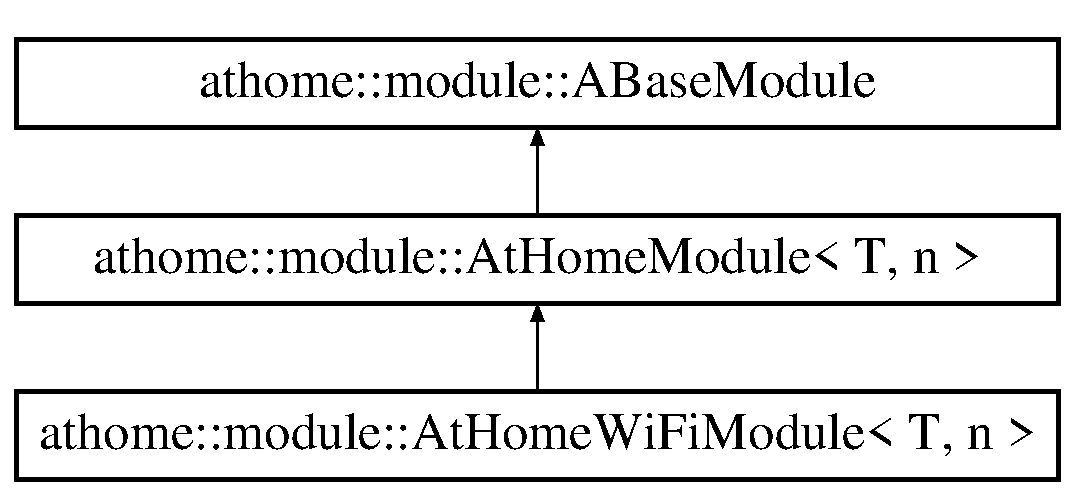
\includegraphics[height=3.000000cm]{classathome_1_1module_1_1_a_base_module}
\end{center}
\end{figure}
\subsection*{Public Member Functions}
\begin{DoxyCompactItemize}
\item 
\mbox{\Hypertarget{classathome_1_1module_1_1_a_base_module_ac1444e438bcfcc06f6593e3d4d5fb1fe}\label{classathome_1_1module_1_1_a_base_module_ac1444e438bcfcc06f6593e3d4d5fb1fe}} 
\mbox{\hyperlink{classathome_1_1module_1_1_a_base_module}{A\+Base\+Module}} \& {\bfseries operator=} (\mbox{\hyperlink{classathome_1_1module_1_1_a_base_module}{A\+Base\+Module}} \&)=delete
\item 
Stream $\ast$$\ast$ \mbox{\hyperlink{classathome_1_1module_1_1_a_base_module_adc612512d2acb7bc3f3d533bcc1aa41b}{get\+Streams}} ()
\item 
void \mbox{\hyperlink{classathome_1_1module_1_1_a_base_module_af1af8e6110a8d0baee15efb2275ae5ae}{set\+Streams}} (Stream $\ast$$\ast$)
\item 
\mbox{\hyperlink{classathome_1_1display_1_1_i_display}{display\+::\+I\+Display}} $\ast$ \mbox{\hyperlink{classathome_1_1module_1_1_a_base_module_ada20b6ad1e6f750d2886f1e7b10cca70}{get\+Display}} ()
\item 
void \mbox{\hyperlink{classathome_1_1module_1_1_a_base_module_a451a1fb99905c7d21f3a818ee39acc69}{set\+Display}} (\mbox{\hyperlink{classathome_1_1display_1_1_i_display}{display\+::\+I\+Display}} $\ast$)
\item 
\mbox{\hyperlink{classathome_1_1power_1_1_i_power}{power\+::\+I\+Power}} $\ast$ \mbox{\hyperlink{classathome_1_1module_1_1_a_base_module_a3152f721f953e32a1f965856936d188e}{get\+Power\+Source}} ()
\item 
void \mbox{\hyperlink{classathome_1_1module_1_1_a_base_module_a0c217f9a8d052efc5490bc9145fdf7f9}{set\+Power\+Source}} (\mbox{\hyperlink{classathome_1_1power_1_1_i_power}{power\+::\+I\+Power}} $\ast$)
\item 
\mbox{\hyperlink{classathome_1_1sensor_1_1_i_sensor}{sensor\+::\+I\+Sensor}} $\ast$ \mbox{\hyperlink{classathome_1_1module_1_1_a_base_module_abd4cf0d059639c4d09f35d7b1ddd2b4e}{get\+Sensor}} ()
\item 
void \mbox{\hyperlink{classathome_1_1module_1_1_a_base_module_a071b5d07dc3497908520a5b0dc9404ef}{set\+Sensor}} (\mbox{\hyperlink{classathome_1_1sensor_1_1_i_sensor}{sensor\+::\+I\+Sensor}} $\ast$)
\item 
\mbox{\hyperlink{classathome_1_1storage_1_1_i_storage}{storage\+::\+I\+Storage}} $\ast$ \mbox{\hyperlink{classathome_1_1module_1_1_a_base_module_accc6c7f840dab1b1e67fe910c833f0b7}{get\+Storage}} ()
\item 
void \mbox{\hyperlink{classathome_1_1module_1_1_a_base_module_a91e714579636e6f4a3628a23a8ba61e7}{set\+Storage}} (\mbox{\hyperlink{classathome_1_1storage_1_1_i_storage}{storage\+::\+I\+Storage}} $\ast$)
\end{DoxyCompactItemize}
\subsection*{Protected Member Functions}
\begin{DoxyCompactItemize}
\item 
\mbox{\Hypertarget{classathome_1_1module_1_1_a_base_module_a7332012b2348fc3a945f9ec9db5d79ca}\label{classathome_1_1module_1_1_a_base_module_a7332012b2348fc3a945f9ec9db5d79ca}} 
{\bfseries A\+Base\+Module} (\mbox{\hyperlink{classathome_1_1display_1_1_i_display}{display\+::\+I\+Display}} $\ast$=nullptr, Stream $\ast$$\ast$=nullptr, \mbox{\hyperlink{classathome_1_1power_1_1_i_power}{power\+::\+I\+Power}} $\ast$=nullptr, \mbox{\hyperlink{classathome_1_1sensor_1_1_i_sensor}{sensor\+::\+I\+Sensor}} $\ast$=nullptr, \mbox{\hyperlink{classathome_1_1storage_1_1_i_storage}{storage\+::\+I\+Storage}} $\ast$=nullptr)
\item 
\mbox{\Hypertarget{classathome_1_1module_1_1_a_base_module_ae2c52cb3313abb5ceb3c7bdb854e9850}\label{classathome_1_1module_1_1_a_base_module_ae2c52cb3313abb5ceb3c7bdb854e9850}} 
{\bfseries A\+Base\+Module} (\mbox{\hyperlink{classathome_1_1module_1_1_a_base_module}{A\+Base\+Module}} \&)=delete
\end{DoxyCompactItemize}
\subsection*{Protected Attributes}
\begin{DoxyCompactItemize}
\item 
\mbox{\Hypertarget{classathome_1_1module_1_1_a_base_module_a1abf0c4e3eeb4824582f79a1d18c2b4c}\label{classathome_1_1module_1_1_a_base_module_a1abf0c4e3eeb4824582f79a1d18c2b4c}} 
\mbox{\hyperlink{classathome_1_1display_1_1_i_display}{display\+::\+I\+Display}} $\ast$ {\bfseries \+\_\+display}
\item 
\mbox{\Hypertarget{classathome_1_1module_1_1_a_base_module_a895fb5050ad2395c25a2e2b6f6e11986}\label{classathome_1_1module_1_1_a_base_module_a895fb5050ad2395c25a2e2b6f6e11986}} 
Stream $\ast$$\ast$ {\bfseries \+\_\+streams}
\item 
\mbox{\Hypertarget{classathome_1_1module_1_1_a_base_module_ae4d60b3b0a69540cdef4bb1db08782ad}\label{classathome_1_1module_1_1_a_base_module_ae4d60b3b0a69540cdef4bb1db08782ad}} 
\mbox{\hyperlink{classathome_1_1power_1_1_i_power}{power\+::\+I\+Power}} $\ast$ {\bfseries \+\_\+power}
\item 
\mbox{\Hypertarget{classathome_1_1module_1_1_a_base_module_ae1a2e5cb4bd4a76cdf248c19110bd3ba}\label{classathome_1_1module_1_1_a_base_module_ae1a2e5cb4bd4a76cdf248c19110bd3ba}} 
\mbox{\hyperlink{classathome_1_1sensor_1_1_i_sensor}{sensor\+::\+I\+Sensor}} $\ast$ {\bfseries \+\_\+sensor}
\item 
\mbox{\Hypertarget{classathome_1_1module_1_1_a_base_module_aa62dad921ff7db37a8501aa827f73e4f}\label{classathome_1_1module_1_1_a_base_module_aa62dad921ff7db37a8501aa827f73e4f}} 
\mbox{\hyperlink{classathome_1_1storage_1_1_i_storage}{storage\+::\+I\+Storage}} $\ast$ {\bfseries \+\_\+storage}
\end{DoxyCompactItemize}


\subsection{Detailed Description}
Abstract base class for all Module classes, mainly handling low level logic and accessers to Module components 

\subsection{Member Function Documentation}
\mbox{\Hypertarget{classathome_1_1module_1_1_a_base_module_ada20b6ad1e6f750d2886f1e7b10cca70}\label{classathome_1_1module_1_1_a_base_module_ada20b6ad1e6f750d2886f1e7b10cca70}} 
\index{athome\+::module\+::\+A\+Base\+Module@{athome\+::module\+::\+A\+Base\+Module}!get\+Display@{get\+Display}}
\index{get\+Display@{get\+Display}!athome\+::module\+::\+A\+Base\+Module@{athome\+::module\+::\+A\+Base\+Module}}
\subsubsection{\texorpdfstring{get\+Display()}{getDisplay()}}
{\footnotesize\ttfamily \mbox{\hyperlink{classathome_1_1display_1_1_i_display}{display\+::\+I\+Display}} $\ast$ athome\+::module\+::\+A\+Base\+Module\+::get\+Display (\begin{DoxyParamCaption}{ }\end{DoxyParamCaption})}

Return a \mbox{\hyperlink{classathome_1_1display_1_1_i_display}{athome\+::display\+::\+I\+Display}} interface pointer on the display currently used by the module.

Warning\+: On some embedded targets there\textquotesingle{}s no C++ runtime (so no {\ttfamily dynamic\+\_\+cast} or {\ttfamily typeof}), the user will have to know and cast by himself this pointer to the correct type.

If there\textquotesingle{}s no display interface currently used by the module, this method returns {\ttfamily nullptr}. \mbox{\Hypertarget{classathome_1_1module_1_1_a_base_module_a3152f721f953e32a1f965856936d188e}\label{classathome_1_1module_1_1_a_base_module_a3152f721f953e32a1f965856936d188e}} 
\index{athome\+::module\+::\+A\+Base\+Module@{athome\+::module\+::\+A\+Base\+Module}!get\+Power\+Source@{get\+Power\+Source}}
\index{get\+Power\+Source@{get\+Power\+Source}!athome\+::module\+::\+A\+Base\+Module@{athome\+::module\+::\+A\+Base\+Module}}
\subsubsection{\texorpdfstring{get\+Power\+Source()}{getPowerSource()}}
{\footnotesize\ttfamily \mbox{\hyperlink{classathome_1_1power_1_1_i_power}{power\+::\+I\+Power}} $\ast$ athome\+::module\+::\+A\+Base\+Module\+::get\+Power\+Source (\begin{DoxyParamCaption}{ }\end{DoxyParamCaption})}

Return a \mbox{\hyperlink{classathome_1_1power_1_1_i_power}{athome\+::power\+::\+I\+Power}} interface pointer on the power supply currently used by the module.

Warning\+: On some embedded targets there\textquotesingle{}s no C++ runtime (so no {\ttfamily dynamic\+\_\+cast} or {\ttfamily typeof}), the user will have to know and cast by himself this pointer to the correct type.

If there\textquotesingle{}s no power interface currently used by the module, this method returns {\ttfamily nullptr}. \mbox{\Hypertarget{classathome_1_1module_1_1_a_base_module_abd4cf0d059639c4d09f35d7b1ddd2b4e}\label{classathome_1_1module_1_1_a_base_module_abd4cf0d059639c4d09f35d7b1ddd2b4e}} 
\index{athome\+::module\+::\+A\+Base\+Module@{athome\+::module\+::\+A\+Base\+Module}!get\+Sensor@{get\+Sensor}}
\index{get\+Sensor@{get\+Sensor}!athome\+::module\+::\+A\+Base\+Module@{athome\+::module\+::\+A\+Base\+Module}}
\subsubsection{\texorpdfstring{get\+Sensor()}{getSensor()}}
{\footnotesize\ttfamily \mbox{\hyperlink{classathome_1_1sensor_1_1_i_sensor}{sensor\+::\+I\+Sensor}} $\ast$ athome\+::module\+::\+A\+Base\+Module\+::get\+Sensor (\begin{DoxyParamCaption}{ }\end{DoxyParamCaption})}

Return a \mbox{\hyperlink{classathome_1_1sensor_1_1_i_sensor}{athome\+::sensor\+::\+I\+Sensor}} interface pointer on the sensor currently used by the module.

Warning\+: On some embedded targets there\textquotesingle{}s no C++ runtime (so no {\ttfamily dynamic\+\_\+cast} or {\ttfamily typeof}), the user will have to know and cast by himself this pointer to the correct type.

If there\textquotesingle{}s no sensor interface currently used by the module, this method returns {\ttfamily nullptr}. \mbox{\Hypertarget{classathome_1_1module_1_1_a_base_module_accc6c7f840dab1b1e67fe910c833f0b7}\label{classathome_1_1module_1_1_a_base_module_accc6c7f840dab1b1e67fe910c833f0b7}} 
\index{athome\+::module\+::\+A\+Base\+Module@{athome\+::module\+::\+A\+Base\+Module}!get\+Storage@{get\+Storage}}
\index{get\+Storage@{get\+Storage}!athome\+::module\+::\+A\+Base\+Module@{athome\+::module\+::\+A\+Base\+Module}}
\subsubsection{\texorpdfstring{get\+Storage()}{getStorage()}}
{\footnotesize\ttfamily \mbox{\hyperlink{classathome_1_1storage_1_1_i_storage}{storage\+::\+I\+Storage}} $\ast$ athome\+::module\+::\+A\+Base\+Module\+::get\+Storage (\begin{DoxyParamCaption}{ }\end{DoxyParamCaption})}

Return a \mbox{\hyperlink{classathome_1_1storage_1_1_i_storage}{athome\+::storage\+::\+I\+Storage}} interface pointer on the storage currently used by the module.

Warning\+: On some embedded targets there\textquotesingle{}s no C++ runtime (so no {\ttfamily dynamic\+\_\+cast} or {\ttfamily typeof}), the user will have to know and cast by himself this pointer to the correct type.

If there\textquotesingle{}s no storage interface currently used by the module, this method returns {\ttfamily nullptr}. \mbox{\Hypertarget{classathome_1_1module_1_1_a_base_module_adc612512d2acb7bc3f3d533bcc1aa41b}\label{classathome_1_1module_1_1_a_base_module_adc612512d2acb7bc3f3d533bcc1aa41b}} 
\index{athome\+::module\+::\+A\+Base\+Module@{athome\+::module\+::\+A\+Base\+Module}!get\+Streams@{get\+Streams}}
\index{get\+Streams@{get\+Streams}!athome\+::module\+::\+A\+Base\+Module@{athome\+::module\+::\+A\+Base\+Module}}
\subsubsection{\texorpdfstring{get\+Streams()}{getStreams()}}
{\footnotesize\ttfamily Stream $\ast$$\ast$ athome\+::module\+::\+A\+Base\+Module\+::get\+Streams (\begin{DoxyParamCaption}{ }\end{DoxyParamCaption})}

Return an array of pointers on {\ttfamily Stream} derived objects terminated by a {\ttfamily nullptr}.

For example, the array can be like this\+: {\ttfamily \{\&Serial, \&Serial1, \&\mbox{\hyperlink{classathome_1_1communication_1_1wifi_1_1_e_s_p8266_wi_fi_communicator}{athome\+::communication\+::wifi\+::\+E\+S\+P8266\+Wi\+Fi\+Communicator}}, nullptr\}}

If there\textquotesingle{}s no {\ttfamily Stream}s used by the module, this method returns {\ttfamily nullptr} \mbox{\Hypertarget{classathome_1_1module_1_1_a_base_module_a451a1fb99905c7d21f3a818ee39acc69}\label{classathome_1_1module_1_1_a_base_module_a451a1fb99905c7d21f3a818ee39acc69}} 
\index{athome\+::module\+::\+A\+Base\+Module@{athome\+::module\+::\+A\+Base\+Module}!set\+Display@{set\+Display}}
\index{set\+Display@{set\+Display}!athome\+::module\+::\+A\+Base\+Module@{athome\+::module\+::\+A\+Base\+Module}}
\subsubsection{\texorpdfstring{set\+Display()}{setDisplay()}}
{\footnotesize\ttfamily void athome\+::module\+::\+A\+Base\+Module\+::set\+Display (\begin{DoxyParamCaption}\item[{\mbox{\hyperlink{classathome_1_1display_1_1_i_display}{display\+::\+I\+Display}} $\ast$}]{display }\end{DoxyParamCaption})}

Set the pointer on the \mbox{\hyperlink{classathome_1_1display_1_1_i_display}{athome\+::display\+::\+I\+Display}} interface used by the module.

Example on Arduino to use a common cathode R\+GB L\+ED and the implementation \mbox{\hyperlink{classathome_1_1module_1_1_at_home_module}{athome\+::module\+::\+At\+Home\+Module}} of this class\+:


\begin{DoxyCode}
\textcolor{preprocessor}{#include <AtHome.h>}

CommonCathodeRGBLed led(2, 3, 4); \textcolor{comment}{// Create a common cathode LED object and defining the pins connected to
       red, green and blue anodes of the LED}
AtHomeModule<uint16\_t, 15> *module = \mbox{\hyperlink{classathome_1_1module_1_1_at_home_module_acc6e7fc0d86f11648fd81729484e546f}{AtHomeModule<uint16\_t, 15>::getInstance}}
      (); \textcolor{comment}{// Create a AtHomeModule instance able to buffer 15 measures from an analog sensor}

\textcolor{keywordtype}{void} setup() \{
  module->setDisplay(&led);
\}

\textcolor{keywordtype}{void} loop() \{
\}
\end{DoxyCode}
 \mbox{\Hypertarget{classathome_1_1module_1_1_a_base_module_a0c217f9a8d052efc5490bc9145fdf7f9}\label{classathome_1_1module_1_1_a_base_module_a0c217f9a8d052efc5490bc9145fdf7f9}} 
\index{athome\+::module\+::\+A\+Base\+Module@{athome\+::module\+::\+A\+Base\+Module}!set\+Power\+Source@{set\+Power\+Source}}
\index{set\+Power\+Source@{set\+Power\+Source}!athome\+::module\+::\+A\+Base\+Module@{athome\+::module\+::\+A\+Base\+Module}}
\subsubsection{\texorpdfstring{set\+Power\+Source()}{setPowerSource()}}
{\footnotesize\ttfamily void athome\+::module\+::\+A\+Base\+Module\+::set\+Power\+Source (\begin{DoxyParamCaption}\item[{\mbox{\hyperlink{classathome_1_1power_1_1_i_power}{power\+::\+I\+Power}} $\ast$}]{power }\end{DoxyParamCaption})}

Set the pointer on the \mbox{\hyperlink{classathome_1_1power_1_1_i_power}{athome\+::power\+::\+I\+Power}} interface used by the module.

For now, there is now implementation of \mbox{\hyperlink{classathome_1_1power_1_1_i_power}{athome\+::power\+::\+I\+Power}} in the library. \mbox{\Hypertarget{classathome_1_1module_1_1_a_base_module_a071b5d07dc3497908520a5b0dc9404ef}\label{classathome_1_1module_1_1_a_base_module_a071b5d07dc3497908520a5b0dc9404ef}} 
\index{athome\+::module\+::\+A\+Base\+Module@{athome\+::module\+::\+A\+Base\+Module}!set\+Sensor@{set\+Sensor}}
\index{set\+Sensor@{set\+Sensor}!athome\+::module\+::\+A\+Base\+Module@{athome\+::module\+::\+A\+Base\+Module}}
\subsubsection{\texorpdfstring{set\+Sensor()}{setSensor()}}
{\footnotesize\ttfamily void athome\+::module\+::\+A\+Base\+Module\+::set\+Sensor (\begin{DoxyParamCaption}\item[{\mbox{\hyperlink{classathome_1_1sensor_1_1_i_sensor}{sensor\+::\+I\+Sensor}} $\ast$}]{sensor }\end{DoxyParamCaption})}

Set the pointer on the \mbox{\hyperlink{classathome_1_1sensor_1_1_i_sensor}{athome\+::sensor\+::\+I\+Sensor}} interface used by the module.

Example on Arduino using the generic Analog\+Sensor class to get measures from a sensor and the implementation \mbox{\hyperlink{classathome_1_1module_1_1_at_home_module}{athome\+::module\+::\+At\+Home\+Module}} of this class\+:


\begin{DoxyCode}
\textcolor{preprocessor}{#include <AtHome.h>}

AtHomeModule<uint16\_t, 15> *module = AtHomeModule::<uint16\_t, 15>::getInstance(); \textcolor{comment}{// Create a AtHomeModule
       instance able to buffer 15 measures from an analog sensor}
AnalogSensor sensor(A0); \textcolor{comment}{// Create an object AnalogSensor reading a sensor on pin A0 of an Arduino}

\textcolor{keywordtype}{void} setup() \{
  module->setSensor(&sensor);
\}

\textcolor{keywordtype}{void} loop() \{
\}
\end{DoxyCode}
 \mbox{\Hypertarget{classathome_1_1module_1_1_a_base_module_a91e714579636e6f4a3628a23a8ba61e7}\label{classathome_1_1module_1_1_a_base_module_a91e714579636e6f4a3628a23a8ba61e7}} 
\index{athome\+::module\+::\+A\+Base\+Module@{athome\+::module\+::\+A\+Base\+Module}!set\+Storage@{set\+Storage}}
\index{set\+Storage@{set\+Storage}!athome\+::module\+::\+A\+Base\+Module@{athome\+::module\+::\+A\+Base\+Module}}
\subsubsection{\texorpdfstring{set\+Storage()}{setStorage()}}
{\footnotesize\ttfamily void athome\+::module\+::\+A\+Base\+Module\+::set\+Storage (\begin{DoxyParamCaption}\item[{\mbox{\hyperlink{classathome_1_1storage_1_1_i_storage}{storage\+::\+I\+Storage}} $\ast$}]{storage }\end{DoxyParamCaption})}

Set the pointer on the \mbox{\hyperlink{classathome_1_1storage_1_1_i_storage}{athome\+::storage\+::\+I\+Storage}} interface used by the module.

Example on an A\+VR Arduino (like Uno, Pro Mini, Nano, Micro, Leonardo, Mega) using the implementation \mbox{\hyperlink{classathome_1_1module_1_1_at_home_module}{athome\+::module\+::\+At\+Home\+Module}} of this class and the Arduino\+E\+E\+P\+R\+OM class to enable storage on the internal E\+E\+P\+R\+OM of these boards\+:


\begin{DoxyCode}
\textcolor{preprocessor}{#include <AtHome.h>}

AtHomeModule<uint16\_t, 15> *module = AtHomeModule::<uint16\_t, 15>::getInstance(); \textcolor{comment}{// Create a AtHomeModule
       instance able to buffer 15 measures from an analog sensor}
ArduinoEEPROM eeprom;

\textcolor{keywordtype}{void} setup() \{
  module->setStorage(&eeprom);
\}

\textcolor{keywordtype}{void} loop() \{
\}
\end{DoxyCode}
 \mbox{\Hypertarget{classathome_1_1module_1_1_a_base_module_af1af8e6110a8d0baee15efb2275ae5ae}\label{classathome_1_1module_1_1_a_base_module_af1af8e6110a8d0baee15efb2275ae5ae}} 
\index{athome\+::module\+::\+A\+Base\+Module@{athome\+::module\+::\+A\+Base\+Module}!set\+Streams@{set\+Streams}}
\index{set\+Streams@{set\+Streams}!athome\+::module\+::\+A\+Base\+Module@{athome\+::module\+::\+A\+Base\+Module}}
\subsubsection{\texorpdfstring{set\+Streams()}{setStreams()}}
{\footnotesize\ttfamily void athome\+::module\+::\+A\+Base\+Module\+::set\+Streams (\begin{DoxyParamCaption}\item[{Stream $\ast$$\ast$}]{streams }\end{DoxyParamCaption})}

Set the array of pointers on Stream derived objects used by module for communications.


\begin{DoxyParams}{Parameters}
{\em streams} & N\+U\+LL terminated array of pointers on Stream instances\\
\hline
\end{DoxyParams}
For example\+: {\ttfamily Stream $\ast$my\+\_\+array\mbox{[}\mbox{]} = \{\&Serial, \&Serial1, \&\mbox{\hyperlink{classathome_1_1communication_1_1wifi_1_1_e_s_p8266_wi_fi_communicator}{athome\+::communication\+::wifi\+::\+E\+S\+P8266\+Wi\+Fi\+Communicator}}, nullptr\};}

Example on Arduino with the implementation \mbox{\hyperlink{classathome_1_1module_1_1_at_home_module}{athome\+::module\+::\+At\+Home\+Module}} of this class\+:


\begin{DoxyCode}
\textcolor{preprocessor}{#include <AtHome.h>}

AtHomeModule<uint16\_t, 15> *module = AtHomeModule::<uint16\_t, 15>::getInstance(); \textcolor{comment}{// Create a AtHomeModule
       instance able to buffer 15 measures from an analog sensor}

\textcolor{keywordtype}{void} setup() \{
  Stream *streams[] = \{&Serial, \textcolor{keyword}{nullptr}\};
  module->setStreams(streams);
\}

\textcolor{keywordtype}{void} loop() \{
\}
\end{DoxyCode}
 

The documentation for this class was generated from the following files\+:\begin{DoxyCompactItemize}
\item 
A\+Base\+Module.\+hpp\item 
A\+Base\+Module.\+cpp\end{DoxyCompactItemize}

\hypertarget{classathome_1_1sensor_1_1_a_humidity_sensor}{}\section{athome\+:\+:sensor\+:\+:A\+Humidity\+Sensor Class Reference}
\label{classathome_1_1sensor_1_1_a_humidity_sensor}\index{athome\+::sensor\+::\+A\+Humidity\+Sensor@{athome\+::sensor\+::\+A\+Humidity\+Sensor}}
Inheritance diagram for athome\+:\+:sensor\+:\+:A\+Humidity\+Sensor\+:\begin{figure}[H]
\begin{center}
\leavevmode
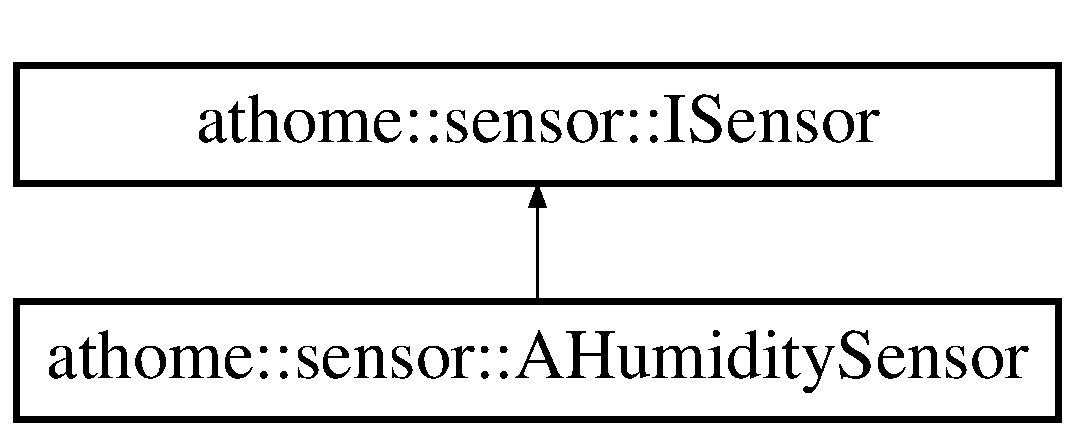
\includegraphics[height=2.000000cm]{classathome_1_1sensor_1_1_a_humidity_sensor}
\end{center}
\end{figure}
\subsection*{Public Member Functions}
\begin{DoxyCompactItemize}
\item 
\mbox{\Hypertarget{classathome_1_1sensor_1_1_a_humidity_sensor_aec2205040170bbf3c64fb1baf797795f}\label{classathome_1_1sensor_1_1_a_humidity_sensor_aec2205040170bbf3c64fb1baf797795f}} 
{\bfseries A\+Humidity\+Sensor} (const \mbox{\hyperlink{classathome_1_1sensor_1_1_a_humidity_sensor}{A\+Humidity\+Sensor}} \&)=delete
\item 
\mbox{\Hypertarget{classathome_1_1sensor_1_1_a_humidity_sensor_a530ebce44ecb090d32ab5450776f3c07}\label{classathome_1_1sensor_1_1_a_humidity_sensor_a530ebce44ecb090d32ab5450776f3c07}} 
\mbox{\hyperlink{classathome_1_1sensor_1_1_a_humidity_sensor}{A\+Humidity\+Sensor}} \& {\bfseries operator=} (const \mbox{\hyperlink{classathome_1_1sensor_1_1_a_humidity_sensor}{A\+Humidity\+Sensor}} \&)=delete
\item 
const \mbox{\hyperlink{structathome_1_1sensor_1_1_i_sensor_1_1_i_sensor_value}{I\+Sensor\+Value}} \& \mbox{\hyperlink{classathome_1_1sensor_1_1_a_humidity_sensor_a7af4527c70b539bec58cecfaae0aa80e}{get\+Sample}} ()
\item 
virtual int32\+\_\+t \mbox{\hyperlink{classathome_1_1sensor_1_1_a_humidity_sensor_a1eb32658be5cfc700523e74387e86053}{get\+Sensor\+Sample}} () const =0
\item 
void \mbox{\hyperlink{classathome_1_1sensor_1_1_a_humidity_sensor_a1a19bfee3db6b0940f1329b42d7ed0d0}{set\+Thresholds}} (const \mbox{\hyperlink{structathome_1_1sensor_1_1_i_sensor_1_1_i_sensor_thresholds}{I\+Sensor\+Thresholds}} \&)
\end{DoxyCompactItemize}
\subsection*{Additional Inherited Members}


\subsection{Member Function Documentation}
\mbox{\Hypertarget{classathome_1_1sensor_1_1_a_humidity_sensor_a7af4527c70b539bec58cecfaae0aa80e}\label{classathome_1_1sensor_1_1_a_humidity_sensor_a7af4527c70b539bec58cecfaae0aa80e}} 
\index{athome\+::sensor\+::\+A\+Humidity\+Sensor@{athome\+::sensor\+::\+A\+Humidity\+Sensor}!get\+Sample@{get\+Sample}}
\index{get\+Sample@{get\+Sample}!athome\+::sensor\+::\+A\+Humidity\+Sensor@{athome\+::sensor\+::\+A\+Humidity\+Sensor}}
\subsubsection{\texorpdfstring{get\+Sample()}{getSample()}}
{\footnotesize\ttfamily const \mbox{\hyperlink{structathome_1_1sensor_1_1_i_sensor_1_1_i_sensor_value}{I\+Sensor\+::\+I\+Sensor\+Value}} \& athome\+::sensor\+::\+A\+Humidity\+Sensor\+::get\+Sample (\begin{DoxyParamCaption}{ }\end{DoxyParamCaption})\hspace{0.3cm}{\ttfamily [virtual]}}

Returns a reference on the sample of the sensor

Return an estimation of the humidity inside the room

Values are from \href{https://www.jechange.fr/energie/duale/guides/thermostat-temperature-4101}{\tt https\+://www.\+jechange.\+fr/energie/duale/guides/thermostat-\/temperature-\/4101} \begin{DoxyReturn}{Returns}
estimation of humidity quality on a scale from 1 (worst) to 10 (best) 
\end{DoxyReturn}


Implements \mbox{\hyperlink{classathome_1_1sensor_1_1_i_sensor_ae109cd3741ea9c88dc7e4f2eaf1485d5}{athome\+::sensor\+::\+I\+Sensor}}.

\mbox{\Hypertarget{classathome_1_1sensor_1_1_a_humidity_sensor_a1eb32658be5cfc700523e74387e86053}\label{classathome_1_1sensor_1_1_a_humidity_sensor_a1eb32658be5cfc700523e74387e86053}} 
\index{athome\+::sensor\+::\+A\+Humidity\+Sensor@{athome\+::sensor\+::\+A\+Humidity\+Sensor}!get\+Sensor\+Sample@{get\+Sensor\+Sample}}
\index{get\+Sensor\+Sample@{get\+Sensor\+Sample}!athome\+::sensor\+::\+A\+Humidity\+Sensor@{athome\+::sensor\+::\+A\+Humidity\+Sensor}}
\subsubsection{\texorpdfstring{get\+Sensor\+Sample()}{getSensorSample()}}
{\footnotesize\ttfamily virtual int32\+\_\+t athome\+::sensor\+::\+A\+Humidity\+Sensor\+::get\+Sensor\+Sample (\begin{DoxyParamCaption}{ }\end{DoxyParamCaption}) const\hspace{0.3cm}{\ttfamily [pure virtual]}}

Returns the last value sampled from the sensor expected to be in micro RH \mbox{\Hypertarget{classathome_1_1sensor_1_1_a_humidity_sensor_a1a19bfee3db6b0940f1329b42d7ed0d0}\label{classathome_1_1sensor_1_1_a_humidity_sensor_a1a19bfee3db6b0940f1329b42d7ed0d0}} 
\index{athome\+::sensor\+::\+A\+Humidity\+Sensor@{athome\+::sensor\+::\+A\+Humidity\+Sensor}!set\+Thresholds@{set\+Thresholds}}
\index{set\+Thresholds@{set\+Thresholds}!athome\+::sensor\+::\+A\+Humidity\+Sensor@{athome\+::sensor\+::\+A\+Humidity\+Sensor}}
\subsubsection{\texorpdfstring{set\+Thresholds()}{setThresholds()}}
{\footnotesize\ttfamily void athome\+::sensor\+::\+A\+Humidity\+Sensor\+::set\+Thresholds (\begin{DoxyParamCaption}\item[{const \mbox{\hyperlink{structathome_1_1sensor_1_1_i_sensor_1_1_i_sensor_thresholds}{I\+Sensor\+Thresholds}} \&}]{ }\end{DoxyParamCaption})\hspace{0.3cm}{\ttfamily [virtual]}}

Returns the estimation of safety from the current sensor value

Example\+:


\begin{DoxyCode}
\textcolor{keywordtype}{void} my\_function\_telling\_if\_a\_sensor\_value\_is\_good\_or\_not(ISensor &my\_sensor) \{
  \mbox{\hyperlink{classathome_1_1sensor_1_1_i_sensor_aa70bc27a4c17c86caf96cca776541ddf}{ISensorScale}} sensor\_estimate = my\_sensor.getEstimate();
  \textcolor{keywordflow}{if} (sensor\_estimate == ISensor::ZERO) \{
    Serial.println(\textcolor{stringliteral}{"The sensor returned an invalid value"});
  \}
  \textcolor{keywordflow}{else} \textcolor{keywordflow}{if} (sensor\_estimate > ISensor::ZERO && sensor\_estimate < 6) \{
    Serial.println(\textcolor{stringliteral}{"Boouh, it's not good :("});
  \}
  \textcolor{keywordflow}{else} \{
    Serial.println(\textcolor{stringliteral}{"Yaaaay!"});
  \}
\}
\end{DoxyCode}
 

Implements \mbox{\hyperlink{classathome_1_1sensor_1_1_i_sensor_af86df8538fecfcfc670b4adfbbde6abb}{athome\+::sensor\+::\+I\+Sensor}}.



The documentation for this class was generated from the following files\+:\begin{DoxyCompactItemize}
\item 
src/A\+Humidity\+Sensor.\+hpp\item 
src/sensor/humidity/A\+Humidity\+Sensor.\+cpp\end{DoxyCompactItemize}

\hypertarget{classathome_1_1sensor_1_1_a_luminosity_sensor}{}\section{athome\+:\+:sensor\+:\+:A\+Luminosity\+Sensor Class Reference}
\label{classathome_1_1sensor_1_1_a_luminosity_sensor}\index{athome\+::sensor\+::\+A\+Luminosity\+Sensor@{athome\+::sensor\+::\+A\+Luminosity\+Sensor}}
Inheritance diagram for athome\+:\+:sensor\+:\+:A\+Luminosity\+Sensor\+:\begin{figure}[H]
\begin{center}
\leavevmode
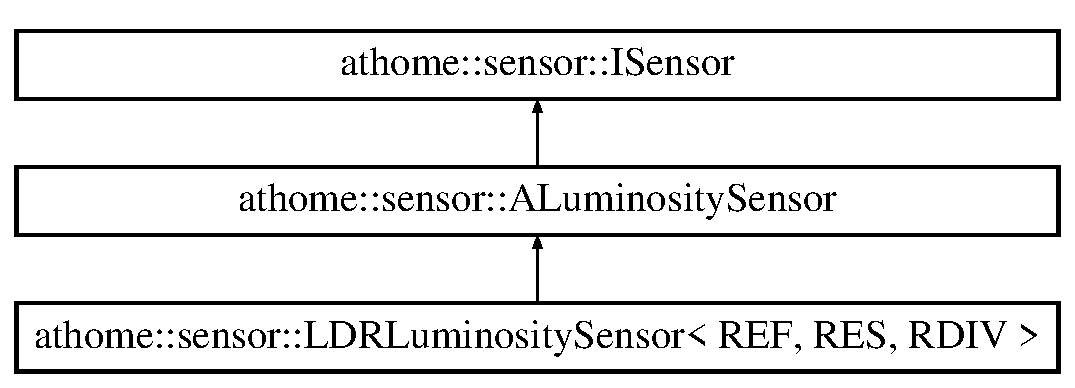
\includegraphics[height=2.000000cm]{classathome_1_1sensor_1_1_a_luminosity_sensor}
\end{center}
\end{figure}
\subsection*{Public Member Functions}
\begin{DoxyCompactItemize}
\item 
\mbox{\Hypertarget{classathome_1_1sensor_1_1_a_luminosity_sensor_a550beb44964597870cd5c94a3485bbaf}\label{classathome_1_1sensor_1_1_a_luminosity_sensor_a550beb44964597870cd5c94a3485bbaf}} 
{\bfseries A\+Luminosity\+Sensor} (const \mbox{\hyperlink{classathome_1_1sensor_1_1_a_luminosity_sensor}{A\+Luminosity\+Sensor}} \&)=delete
\item 
\mbox{\Hypertarget{classathome_1_1sensor_1_1_a_luminosity_sensor_a9a91cdf883f0f06be50a74ec2e73d710}\label{classathome_1_1sensor_1_1_a_luminosity_sensor_a9a91cdf883f0f06be50a74ec2e73d710}} 
\mbox{\hyperlink{classathome_1_1sensor_1_1_a_luminosity_sensor}{A\+Luminosity\+Sensor}} \& {\bfseries operator=} (const \mbox{\hyperlink{classathome_1_1sensor_1_1_a_luminosity_sensor}{A\+Luminosity\+Sensor}} \&)=delete
\item 
virtual uint8\+\_\+t $\ast$ \mbox{\hyperlink{classathome_1_1sensor_1_1_a_luminosity_sensor_a299491729362d34f474094dfd10eb310}{get\+Sample}} ()=0
\item 
virtual uint16\+\_\+t \mbox{\hyperlink{classathome_1_1sensor_1_1_a_luminosity_sensor_a1cc3cee76cd76486c6e6b51ac484cb2a}{get\+Last\+Sample}} () const =0
\item 
virtual \mbox{\hyperlink{classathome_1_1sensor_1_1_i_sensor_aa70bc27a4c17c86caf96cca776541ddf}{I\+Sensor\+Scale}} \mbox{\hyperlink{classathome_1_1sensor_1_1_a_luminosity_sensor_aa6c0e60c108b0494f0132b033ce3dd82}{get\+Estimate}} ()
\end{DoxyCompactItemize}
\subsection*{Additional Inherited Members}


\subsection{Member Function Documentation}
\mbox{\Hypertarget{classathome_1_1sensor_1_1_a_luminosity_sensor_aa6c0e60c108b0494f0132b033ce3dd82}\label{classathome_1_1sensor_1_1_a_luminosity_sensor_aa6c0e60c108b0494f0132b033ce3dd82}} 
\index{athome\+::sensor\+::\+A\+Luminosity\+Sensor@{athome\+::sensor\+::\+A\+Luminosity\+Sensor}!get\+Estimate@{get\+Estimate}}
\index{get\+Estimate@{get\+Estimate}!athome\+::sensor\+::\+A\+Luminosity\+Sensor@{athome\+::sensor\+::\+A\+Luminosity\+Sensor}}
\subsubsection{\texorpdfstring{get\+Estimate()}{getEstimate()}}
{\footnotesize\ttfamily \mbox{\hyperlink{classathome_1_1sensor_1_1_i_sensor_aa70bc27a4c17c86caf96cca776541ddf}{I\+Sensor\+::\+I\+Sensor\+Scale}} athome\+::sensor\+::\+A\+Luminosity\+Sensor\+::get\+Estimate (\begin{DoxyParamCaption}{ }\end{DoxyParamCaption})\hspace{0.3cm}{\ttfamily [virtual]}}

Returns the estimation of safety from the current sensor value

Example\+:


\begin{DoxyCode}
\textcolor{keywordtype}{void} my\_function\_telling\_if\_a\_sensor\_value\_is\_good\_or\_not(ISensor &my\_sensor) \{
  \mbox{\hyperlink{classathome_1_1sensor_1_1_i_sensor_aa70bc27a4c17c86caf96cca776541ddf}{ISensorScale}} sensor\_estimate = my\_sensor.getEstimate();
  \textcolor{keywordflow}{if} (sensor\_estimate == ISensor::ZERO) \{
    Serial.println(\textcolor{stringliteral}{"The sensor returned an invalid value"});
  \}
  \textcolor{keywordflow}{else} \textcolor{keywordflow}{if} (sensor\_estimate > ISensor::ZERO && sensor\_estimate < 6) \{
    Serial.println(\textcolor{stringliteral}{"Boouh, it's not good :("});
  \}
  \textcolor{keywordflow}{else} \{
    Serial.println(\textcolor{stringliteral}{"Yaaaay!"});
  \}
\}
\end{DoxyCode}
 

Implements \mbox{\hyperlink{classathome_1_1sensor_1_1_i_sensor_a95785b54ffe3a8f7e48c81b5732e3b9f}{athome\+::sensor\+::\+I\+Sensor}}.

\mbox{\Hypertarget{classathome_1_1sensor_1_1_a_luminosity_sensor_a1cc3cee76cd76486c6e6b51ac484cb2a}\label{classathome_1_1sensor_1_1_a_luminosity_sensor_a1cc3cee76cd76486c6e6b51ac484cb2a}} 
\index{athome\+::sensor\+::\+A\+Luminosity\+Sensor@{athome\+::sensor\+::\+A\+Luminosity\+Sensor}!get\+Last\+Sample@{get\+Last\+Sample}}
\index{get\+Last\+Sample@{get\+Last\+Sample}!athome\+::sensor\+::\+A\+Luminosity\+Sensor@{athome\+::sensor\+::\+A\+Luminosity\+Sensor}}
\subsubsection{\texorpdfstring{get\+Last\+Sample()}{getLastSample()}}
{\footnotesize\ttfamily virtual uint16\+\_\+t athome\+::sensor\+::\+A\+Luminosity\+Sensor\+::get\+Last\+Sample (\begin{DoxyParamCaption}{ }\end{DoxyParamCaption}) const\hspace{0.3cm}{\ttfamily [pure virtual]}}

Return the number of lux as an integer. \mbox{\Hypertarget{classathome_1_1sensor_1_1_a_luminosity_sensor_a299491729362d34f474094dfd10eb310}\label{classathome_1_1sensor_1_1_a_luminosity_sensor_a299491729362d34f474094dfd10eb310}} 
\index{athome\+::sensor\+::\+A\+Luminosity\+Sensor@{athome\+::sensor\+::\+A\+Luminosity\+Sensor}!get\+Sample@{get\+Sample}}
\index{get\+Sample@{get\+Sample}!athome\+::sensor\+::\+A\+Luminosity\+Sensor@{athome\+::sensor\+::\+A\+Luminosity\+Sensor}}
\subsubsection{\texorpdfstring{get\+Sample()}{getSample()}}
{\footnotesize\ttfamily virtual uint8\+\_\+t$\ast$ athome\+::sensor\+::\+A\+Luminosity\+Sensor\+::get\+Sample (\begin{DoxyParamCaption}{ }\end{DoxyParamCaption})\hspace{0.3cm}{\ttfamily [pure virtual]}}

Return a pointer on a uint16\+\_\+t storing the number of lux as an integer. 

Implements \mbox{\hyperlink{classathome_1_1sensor_1_1_i_sensor_a2513fd8acc5d8251439330ca0e78cf04}{athome\+::sensor\+::\+I\+Sensor}}.



The documentation for this class was generated from the following files\+:\begin{DoxyCompactItemize}
\item 
A\+Luminosity\+Sensor.\+hpp\item 
A\+Luminosity\+Sensor.\+cpp\end{DoxyCompactItemize}

\hypertarget{classathome_1_1sensor_1_1_analog_sensor}{}\section{athome\+:\+:sensor\+:\+:Analog\+Sensor Class Reference}
\label{classathome_1_1sensor_1_1_analog_sensor}\index{athome\+::sensor\+::\+Analog\+Sensor@{athome\+::sensor\+::\+Analog\+Sensor}}


{\ttfamily \#include $<$Analog\+Sensor.\+hpp$>$}

Inheritance diagram for athome\+:\+:sensor\+:\+:Analog\+Sensor\+:\begin{figure}[H]
\begin{center}
\leavevmode
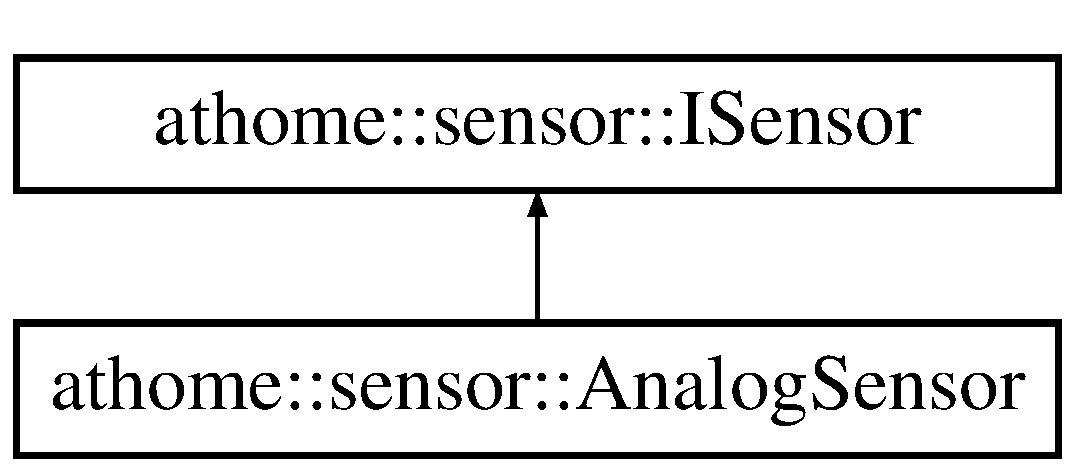
\includegraphics[height=2.000000cm]{classathome_1_1sensor_1_1_analog_sensor}
\end{center}
\end{figure}
\subsection*{Public Member Functions}
\begin{DoxyCompactItemize}
\item 
\mbox{\hyperlink{classathome_1_1sensor_1_1_analog_sensor_acd973b3cf9be02ca318eea594e8732d3}{Analog\+Sensor}} (uint8\+\_\+t pin)
\item 
\mbox{\Hypertarget{classathome_1_1sensor_1_1_analog_sensor_a11abebcdb62ccd8fb7f10e4d1cc91516}\label{classathome_1_1sensor_1_1_analog_sensor_a11abebcdb62ccd8fb7f10e4d1cc91516}} 
{\bfseries Analog\+Sensor} (const \mbox{\hyperlink{classathome_1_1sensor_1_1_analog_sensor}{Analog\+Sensor}} \&)=delete
\item 
\mbox{\Hypertarget{classathome_1_1sensor_1_1_analog_sensor_a3e2cb67bd8eb58798d28eaf152f33b1a}\label{classathome_1_1sensor_1_1_analog_sensor_a3e2cb67bd8eb58798d28eaf152f33b1a}} 
\mbox{\hyperlink{classathome_1_1sensor_1_1_analog_sensor}{Analog\+Sensor}} \& {\bfseries operator=} (const \mbox{\hyperlink{classathome_1_1sensor_1_1_analog_sensor}{Analog\+Sensor}} \&)=delete
\item 
virtual uint8\+\_\+t $\ast$ \mbox{\hyperlink{classathome_1_1sensor_1_1_analog_sensor_ac45070688a9433256a5f847467c251fa}{get\+Sample}} ()
\item 
virtual \mbox{\hyperlink{classathome_1_1sensor_1_1_i_sensor_aa70bc27a4c17c86caf96cca776541ddf}{I\+Sensor\+Scale}} \mbox{\hyperlink{classathome_1_1sensor_1_1_analog_sensor_a728e2f65638f488cd1829c5f318531db}{get\+Estimate}} ()
\item 
uint8\+\_\+t \mbox{\hyperlink{classathome_1_1sensor_1_1_analog_sensor_ac4eab6ad6117e8e6689f9e1d9fb05015}{get\+Analogue\+Pin}} ()
\end{DoxyCompactItemize}
\subsection*{Protected Attributes}
\begin{DoxyCompactItemize}
\item 
\mbox{\Hypertarget{classathome_1_1sensor_1_1_analog_sensor_a06c196fae2f37af456406430651653a9}\label{classathome_1_1sensor_1_1_analog_sensor_a06c196fae2f37af456406430651653a9}} 
uint8\+\_\+t {\bfseries \+\_\+analog\+\_\+pin}
\end{DoxyCompactItemize}
\subsection*{Additional Inherited Members}


\subsection{Detailed Description}
Base class derived from \mbox{\hyperlink{classathome_1_1sensor_1_1_i_sensor}{athome\+::sensor\+::\+I\+Sensor}} allowing to use an analog sensor.

Warning\+: This class is only able to sample an analog sensor, not to interpret its value.

Thus, {\ttfamily get\+Estimate} method will always return athome\+::sensor\+::\+I\+Sensor\+::\+I\+Sensor\+Scale\+::\+Z\+E\+RO if this method is not overriden by a specialized class. 

\subsection{Constructor \& Destructor Documentation}
\mbox{\Hypertarget{classathome_1_1sensor_1_1_analog_sensor_acd973b3cf9be02ca318eea594e8732d3}\label{classathome_1_1sensor_1_1_analog_sensor_acd973b3cf9be02ca318eea594e8732d3}} 
\index{athome\+::sensor\+::\+Analog\+Sensor@{athome\+::sensor\+::\+Analog\+Sensor}!Analog\+Sensor@{Analog\+Sensor}}
\index{Analog\+Sensor@{Analog\+Sensor}!athome\+::sensor\+::\+Analog\+Sensor@{athome\+::sensor\+::\+Analog\+Sensor}}
\subsubsection{\texorpdfstring{Analog\+Sensor()}{AnalogSensor()}}
{\footnotesize\ttfamily athome\+::sensor\+::\+Analog\+Sensor\+::\+Analog\+Sensor (\begin{DoxyParamCaption}\item[{uint8\+\_\+t}]{pin }\end{DoxyParamCaption})}

Create an instance of \mbox{\hyperlink{classathome_1_1sensor_1_1_analog_sensor}{Analog\+Sensor}}, needing the analog pin used to sample the sensor. 

\subsection{Member Function Documentation}
\mbox{\Hypertarget{classathome_1_1sensor_1_1_analog_sensor_ac4eab6ad6117e8e6689f9e1d9fb05015}\label{classathome_1_1sensor_1_1_analog_sensor_ac4eab6ad6117e8e6689f9e1d9fb05015}} 
\index{athome\+::sensor\+::\+Analog\+Sensor@{athome\+::sensor\+::\+Analog\+Sensor}!get\+Analogue\+Pin@{get\+Analogue\+Pin}}
\index{get\+Analogue\+Pin@{get\+Analogue\+Pin}!athome\+::sensor\+::\+Analog\+Sensor@{athome\+::sensor\+::\+Analog\+Sensor}}
\subsubsection{\texorpdfstring{get\+Analogue\+Pin()}{getAnaloguePin()}}
{\footnotesize\ttfamily uint8\+\_\+t athome\+::sensor\+::\+Analog\+Sensor\+::get\+Analogue\+Pin (\begin{DoxyParamCaption}{ }\end{DoxyParamCaption})}

Return the value of the pin used to sample the sensor. \mbox{\Hypertarget{classathome_1_1sensor_1_1_analog_sensor_a728e2f65638f488cd1829c5f318531db}\label{classathome_1_1sensor_1_1_analog_sensor_a728e2f65638f488cd1829c5f318531db}} 
\index{athome\+::sensor\+::\+Analog\+Sensor@{athome\+::sensor\+::\+Analog\+Sensor}!get\+Estimate@{get\+Estimate}}
\index{get\+Estimate@{get\+Estimate}!athome\+::sensor\+::\+Analog\+Sensor@{athome\+::sensor\+::\+Analog\+Sensor}}
\subsubsection{\texorpdfstring{get\+Estimate()}{getEstimate()}}
{\footnotesize\ttfamily \mbox{\hyperlink{classathome_1_1sensor_1_1_i_sensor_aa70bc27a4c17c86caf96cca776541ddf}{I\+Sensor\+::\+I\+Sensor\+Scale}} athome\+::sensor\+::\+Analog\+Sensor\+::get\+Estimate (\begin{DoxyParamCaption}{ }\end{DoxyParamCaption})\hspace{0.3cm}{\ttfamily [virtual]}}

Return athome\+::sensor\+::\+I\+Sensor\+::\+I\+Sensor\+Scale\+::\+Z\+E\+RO if object is an instance of \mbox{\hyperlink{classathome_1_1sensor_1_1_analog_sensor}{Analog\+Sensor}} class 

Implements \mbox{\hyperlink{classathome_1_1sensor_1_1_i_sensor_a95785b54ffe3a8f7e48c81b5732e3b9f}{athome\+::sensor\+::\+I\+Sensor}}.

\mbox{\Hypertarget{classathome_1_1sensor_1_1_analog_sensor_ac45070688a9433256a5f847467c251fa}\label{classathome_1_1sensor_1_1_analog_sensor_ac45070688a9433256a5f847467c251fa}} 
\index{athome\+::sensor\+::\+Analog\+Sensor@{athome\+::sensor\+::\+Analog\+Sensor}!get\+Sample@{get\+Sample}}
\index{get\+Sample@{get\+Sample}!athome\+::sensor\+::\+Analog\+Sensor@{athome\+::sensor\+::\+Analog\+Sensor}}
\subsubsection{\texorpdfstring{get\+Sample()}{getSample()}}
{\footnotesize\ttfamily uint8\+\_\+t $\ast$ athome\+::sensor\+::\+Analog\+Sensor\+::get\+Sample (\begin{DoxyParamCaption}{ }\end{DoxyParamCaption})\hspace{0.3cm}{\ttfamily [virtual]}}

Return a pointer on a {\ttfamily uint16\+\_\+t} variable, so the memory area returned by the pointer is 2 bytes long or equivalent to an array of 2 {\ttfamily uint8\+\_\+t}.

Examples of use\+:


\begin{DoxyCode}
\textcolor{keywordtype}{void} my\_func\_reading\_my\_sensor(ISensor &my\_sensor) \{
  uint8\_t *pointer = my\_sensor.getSample();
  \textcolor{keywordflow}{if} (pointer == \textcolor{keyword}{nullptr}) \{
    \textcolor{comment}{// Invalid pointer -> might be caused by a sample error from the sensor.}
    \textcolor{comment}{// Can't happen with base AnalogSensor class but could happen from other athome::sensor::ISensor
       derived classes, so it's good practice to always check returned pointer.}
    \textcolor{keywordflow}{return};
  \}
  \textcolor{comment}{// Can access value from casting pointer to its original uint16\_t type:}
  uint16\_t *full\_pointer = \textcolor{keyword}{reinterpret\_cast<}uint16\_t *\textcolor{keyword}{>}(pointer);
  \textcolor{comment}{// Or by casting it in C-style:}
  uint16\_t *c\_pointer = (uint16\_t *)pointer;
  \textcolor{comment}{// Or by accessing it as an array of 2 bytes:}
  uint16\_t value = ((pointer[0]) << 8) | pointer[1];

  printf(\textcolor{stringliteral}{"%hu\(\backslash\)n"}, *full\_pointer); \textcolor{comment}{// Or Serial.println(*full\_pointer) for example on Arduino}
  printf(\textcolor{stringliteral}{"%hu\(\backslash\)n"}, *c\_pointer); \textcolor{comment}{// Or Serial.println(*c\_pointer) for example on Arduino}
  printf(\textcolor{stringliteral}{"%hu\(\backslash\)n"}, value); \textcolor{comment}{// Or Serial.println(value) for example on Arduino}
\}
\end{DoxyCode}
 

Implements \mbox{\hyperlink{classathome_1_1sensor_1_1_i_sensor_a2513fd8acc5d8251439330ca0e78cf04}{athome\+::sensor\+::\+I\+Sensor}}.



The documentation for this class was generated from the following files\+:\begin{DoxyCompactItemize}
\item 
Analog\+Sensor.\+hpp\item 
Analog\+Sensor.\+cpp\end{DoxyCompactItemize}

\hypertarget{classathome_1_1communication_1_1_a_network_communicator}{}\section{athome\+:\+:communication\+:\+:A\+Network\+Communicator Class Reference}
\label{classathome_1_1communication_1_1_a_network_communicator}\index{athome\+::communication\+::\+A\+Network\+Communicator@{athome\+::communication\+::\+A\+Network\+Communicator}}
Inheritance diagram for athome\+:\+:communication\+:\+:A\+Network\+Communicator\+:\begin{figure}[H]
\begin{center}
\leavevmode
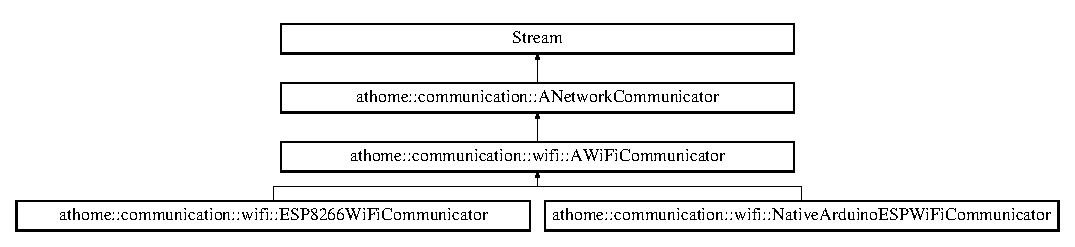
\includegraphics[height=2.871795cm]{classathome_1_1communication_1_1_a_network_communicator}
\end{center}
\end{figure}
\subsection*{Public Member Functions}
\begin{DoxyCompactItemize}
\item 
\mbox{\Hypertarget{classathome_1_1communication_1_1_a_network_communicator_a0c5ca4008e3de2e987d5cafaf9914960}\label{classathome_1_1communication_1_1_a_network_communicator_a0c5ca4008e3de2e987d5cafaf9914960}} 
{\bfseries A\+Network\+Communicator} (\mbox{\hyperlink{structathome_1_1communication_1_1ip_1_1s__host}{ip\+::tcp\+\_\+host}} $\ast$=nullptr)
\item 
\mbox{\Hypertarget{classathome_1_1communication_1_1_a_network_communicator_a3650944e94e130a11bd0167eb55e40c1}\label{classathome_1_1communication_1_1_a_network_communicator_a3650944e94e130a11bd0167eb55e40c1}} 
{\bfseries A\+Network\+Communicator} (const \mbox{\hyperlink{classathome_1_1communication_1_1_a_network_communicator}{A\+Network\+Communicator}} \&)=delete
\item 
\mbox{\Hypertarget{classathome_1_1communication_1_1_a_network_communicator_a3d8984345e39d51da706a02c8d751e6b}\label{classathome_1_1communication_1_1_a_network_communicator_a3d8984345e39d51da706a02c8d751e6b}} 
\mbox{\hyperlink{classathome_1_1communication_1_1_a_network_communicator}{A\+Network\+Communicator}} \& {\bfseries operator=} (const \mbox{\hyperlink{classathome_1_1communication_1_1_a_network_communicator}{A\+Network\+Communicator}} \&)=delete
\item 
virtual int \mbox{\hyperlink{classathome_1_1communication_1_1_a_network_communicator_a2bf367d03c98e8523fda71dd43ffa2fb}{available}} ()=0
\item 
virtual int \mbox{\hyperlink{classathome_1_1communication_1_1_a_network_communicator_a88d3c4366daf48865ab48b22eb62d610}{read}} ()=0
\item 
virtual int \mbox{\hyperlink{classathome_1_1communication_1_1_a_network_communicator_ad06ecdc94aa77b1bab934b85bed2ac7d}{peek}} ()=0
\item 
virtual size\+\_\+t \mbox{\hyperlink{classathome_1_1communication_1_1_a_network_communicator_a87adf68359a4ec5b0a38bea529ebf732}{write}} (uint8\+\_\+t)=0
\item 
virtual void \mbox{\hyperlink{classathome_1_1communication_1_1_a_network_communicator_a5e3b278ad11e6c00ac7d3e2fee3f01b1}{flush}} ()=0
\item 
virtual int \mbox{\hyperlink{classathome_1_1communication_1_1_a_network_communicator_a370176dae8f38225446e83a132dbcff7}{connect\+To\+Host}} ()=0
\item 
virtual int \mbox{\hyperlink{classathome_1_1communication_1_1_a_network_communicator_a025b7fbe9b3c4452fcf1925d766324eb}{disconnect\+From\+Host}} ()=0
\item 
const \mbox{\hyperlink{structathome_1_1communication_1_1ip_1_1s__host}{ip\+::tcp\+\_\+host}} \& \mbox{\hyperlink{classathome_1_1communication_1_1_a_network_communicator_a6b52a87191bef07e73ec1bbba0713080}{get\+Host}} () const
\item 
void \mbox{\hyperlink{classathome_1_1communication_1_1_a_network_communicator_a2c19d9918fc1d85d1768bfd0ae0bd4d4}{set\+Host}} (const \mbox{\hyperlink{structathome_1_1communication_1_1ip_1_1s__host}{ip\+::tcp\+\_\+host}} \&)
\item 
\mbox{\Hypertarget{classathome_1_1communication_1_1_a_network_communicator_a86f8dec086713ed91c398e23c11a49ce}\label{classathome_1_1communication_1_1_a_network_communicator_a86f8dec086713ed91c398e23c11a49ce}} 
bool {\bfseries is\+Host\+Configured} ()
\end{DoxyCompactItemize}
\subsection*{Protected Attributes}
\begin{DoxyCompactItemize}
\item 
\mbox{\Hypertarget{classathome_1_1communication_1_1_a_network_communicator_ad7b22eedcb47003e1b79e8ec480da119}\label{classathome_1_1communication_1_1_a_network_communicator_ad7b22eedcb47003e1b79e8ec480da119}} 
\mbox{\hyperlink{structathome_1_1communication_1_1ip_1_1s__host}{ip\+::tcp\+\_\+host}} {\bfseries \+\_\+host}
\end{DoxyCompactItemize}


\subsection{Member Function Documentation}
\mbox{\Hypertarget{classathome_1_1communication_1_1_a_network_communicator_a2bf367d03c98e8523fda71dd43ffa2fb}\label{classathome_1_1communication_1_1_a_network_communicator_a2bf367d03c98e8523fda71dd43ffa2fb}} 
\index{athome\+::communication\+::\+A\+Network\+Communicator@{athome\+::communication\+::\+A\+Network\+Communicator}!available@{available}}
\index{available@{available}!athome\+::communication\+::\+A\+Network\+Communicator@{athome\+::communication\+::\+A\+Network\+Communicator}}
\subsubsection{\texorpdfstring{available()}{available()}}
{\footnotesize\ttfamily virtual int athome\+::communication\+::\+A\+Network\+Communicator\+::available (\begin{DoxyParamCaption}{ }\end{DoxyParamCaption})\hspace{0.3cm}{\ttfamily [pure virtual]}}

Virtual method inherited from Stream interface. \mbox{[}See documentation on Arduino reference.\mbox{]}(\href{https://www.arduino.cc/reference/en/language/functions/communication/stream/streamavailable/}{\tt https\+://www.\+arduino.\+cc/reference/en/language/functions/communication/stream/streamavailable/}) 

Implemented in \mbox{\hyperlink{classathome_1_1communication_1_1wifi_1_1_native_arduino_e_s_p_wi_fi_communicator_a6cd3fe64efeb1085c7e6dc71a740a24b}{athome\+::communication\+::wifi\+::\+Native\+Arduino\+E\+S\+P\+Wi\+Fi\+Communicator}}, and \mbox{\hyperlink{classathome_1_1communication_1_1wifi_1_1_e_s_p8266_wi_fi_communicator_af9b1e28910959893748763faaa5373a0}{athome\+::communication\+::wifi\+::\+E\+S\+P8266\+Wi\+Fi\+Communicator}}.

\mbox{\Hypertarget{classathome_1_1communication_1_1_a_network_communicator_a370176dae8f38225446e83a132dbcff7}\label{classathome_1_1communication_1_1_a_network_communicator_a370176dae8f38225446e83a132dbcff7}} 
\index{athome\+::communication\+::\+A\+Network\+Communicator@{athome\+::communication\+::\+A\+Network\+Communicator}!connect\+To\+Host@{connect\+To\+Host}}
\index{connect\+To\+Host@{connect\+To\+Host}!athome\+::communication\+::\+A\+Network\+Communicator@{athome\+::communication\+::\+A\+Network\+Communicator}}
\subsubsection{\texorpdfstring{connect\+To\+Host()}{connectToHost()}}
{\footnotesize\ttfamily virtual int athome\+::communication\+::\+A\+Network\+Communicator\+::connect\+To\+Host (\begin{DoxyParamCaption}{ }\end{DoxyParamCaption})\hspace{0.3cm}{\ttfamily [pure virtual]}}

Virtual method used to connect adapter to a socket on a host.

A return value of 0 is expected to indicate success, otherwise all other values are available for error codes.

Example\+:


\begin{DoxyCode}
\textcolor{preprocessor}{#include <AtHome.h>}

\textcolor{keyword}{using} \mbox{\hyperlink{structathome_1_1communication_1_1ip_1_1s__host}{athome::communication::ip::tcp\_host}}; \textcolor{comment}{// Use this to not have to
       write}
the full \textcolor{keyword}{namespace }names further using
\mbox{\hyperlink{namespaceathome}{athome}}::communication::wifi::WiFi\_client; using
\mbox{\hyperlink{classathome_1_1communication_1_1wifi_1_1_a_wi_fi_communicator}{athome::communication::wifi::AWiFiCommunicator}};

void my\_function\_connecting\_to\_http\_port\_on\_router(AWiFiCommunicator &wifi)
\{ \textcolor{keyword}{const} WiFi\_client &my\_ip = wifi.getConnectionAddresses(); \textcolor{comment}{// Get our}
actual MAC and IP (IPv4 or IPv6) addresses tcp\_host router =
\{\{my\_ip.ipv4[0], my\_ip.ipv4[1], my\_ip.ipv4[2], 1\}, 80\}; \textcolor{comment}{// Use our current}
IPv4 address to deduce the one of the router, which often is the same as
ours but ending with the value 1 wifi.setHost(router); \textcolor{comment}{// Set the new host}
to connect on, our structure tcp\_host is a couple IP + port \textcolor{keywordflow}{if}
(!wifi.connectToHost()) \{ \textcolor{comment}{// Connect to the socket on the host}
    Serial.println(\textcolor{stringliteral}{"Successfully connected to host"});
  \} \textcolor{keywordflow}{else} \{
    Serial.println(\textcolor{stringliteral}{"Failed to connect to host"});
  \}
\}
\end{DoxyCode}
 

Implemented in \mbox{\hyperlink{classathome_1_1communication_1_1wifi_1_1_e_s_p8266_wi_fi_communicator_a159a93b350df135daa967665c9e53e2f}{athome\+::communication\+::wifi\+::\+E\+S\+P8266\+Wi\+Fi\+Communicator}}, and \mbox{\hyperlink{classathome_1_1communication_1_1wifi_1_1_native_arduino_e_s_p_wi_fi_communicator_ab3f6a0e1b9d3be98a876f95dde97976b}{athome\+::communication\+::wifi\+::\+Native\+Arduino\+E\+S\+P\+Wi\+Fi\+Communicator}}.

\mbox{\Hypertarget{classathome_1_1communication_1_1_a_network_communicator_a025b7fbe9b3c4452fcf1925d766324eb}\label{classathome_1_1communication_1_1_a_network_communicator_a025b7fbe9b3c4452fcf1925d766324eb}} 
\index{athome\+::communication\+::\+A\+Network\+Communicator@{athome\+::communication\+::\+A\+Network\+Communicator}!disconnect\+From\+Host@{disconnect\+From\+Host}}
\index{disconnect\+From\+Host@{disconnect\+From\+Host}!athome\+::communication\+::\+A\+Network\+Communicator@{athome\+::communication\+::\+A\+Network\+Communicator}}
\subsubsection{\texorpdfstring{disconnect\+From\+Host()}{disconnectFromHost()}}
{\footnotesize\ttfamily virtual int athome\+::communication\+::\+A\+Network\+Communicator\+::disconnect\+From\+Host (\begin{DoxyParamCaption}{ }\end{DoxyParamCaption})\hspace{0.3cm}{\ttfamily [pure virtual]}}

Virtual method to disconnect from the current host, closing the socket.

A return value of 0 is expected to indicate success, otherwise all other values are available for error codes.

Example\+:


\begin{DoxyCode}
\textcolor{preprocessor}{#include <AWiFiCommunicator.hpp>}

\textcolor{keyword}{using} \mbox{\hyperlink{classathome_1_1communication_1_1wifi_1_1_a_wi_fi_communicator}{athome::communication::wifi::AWiFiCommunicator}};

\textcolor{keywordtype}{void} my\_function\_disconnecting\_an\_adapter\_from\_host(AWiFiCommunicator
&wifi) \{ \textcolor{keywordflow}{if} (!wifi.disconnectFromHost()) \{ Serial.println(\textcolor{stringliteral}{"Successfully}
\textcolor{stringliteral}{disconnected from host"}); \} \textcolor{keywordflow}{else} \{ Serial.println(\textcolor{stringliteral}{"Failed to disconnect}
\textcolor{stringliteral}{from host"}); \textcolor{comment}{// If that happens, see the same scenario on disconnect method}
to have the solution ;)
  \}
\}
\end{DoxyCode}
 

Implemented in \mbox{\hyperlink{classathome_1_1communication_1_1wifi_1_1_e_s_p8266_wi_fi_communicator_a0f8adbe1b1d219148c4f340980056356}{athome\+::communication\+::wifi\+::\+E\+S\+P8266\+Wi\+Fi\+Communicator}}, and \mbox{\hyperlink{classathome_1_1communication_1_1wifi_1_1_native_arduino_e_s_p_wi_fi_communicator_a8fa44a5078cb7d61f01b306e1d0d1bfe}{athome\+::communication\+::wifi\+::\+Native\+Arduino\+E\+S\+P\+Wi\+Fi\+Communicator}}.

\mbox{\Hypertarget{classathome_1_1communication_1_1_a_network_communicator_a5e3b278ad11e6c00ac7d3e2fee3f01b1}\label{classathome_1_1communication_1_1_a_network_communicator_a5e3b278ad11e6c00ac7d3e2fee3f01b1}} 
\index{athome\+::communication\+::\+A\+Network\+Communicator@{athome\+::communication\+::\+A\+Network\+Communicator}!flush@{flush}}
\index{flush@{flush}!athome\+::communication\+::\+A\+Network\+Communicator@{athome\+::communication\+::\+A\+Network\+Communicator}}
\subsubsection{\texorpdfstring{flush()}{flush()}}
{\footnotesize\ttfamily virtual void athome\+::communication\+::\+A\+Network\+Communicator\+::flush (\begin{DoxyParamCaption}{ }\end{DoxyParamCaption})\hspace{0.3cm}{\ttfamily [pure virtual]}}

Virtual method inherited from Stream interface. \mbox{[}See documentation on Arduino reference.\mbox{]}(\href{https://www.arduino.cc/reference/en/language/functions/communication/stream/streamflush/}{\tt https\+://www.\+arduino.\+cc/reference/en/language/functions/communication/stream/streamflush/}) 

Implemented in \mbox{\hyperlink{classathome_1_1communication_1_1wifi_1_1_native_arduino_e_s_p_wi_fi_communicator_a5b02865d3bf418d1b4dff8a1198c8dac}{athome\+::communication\+::wifi\+::\+Native\+Arduino\+E\+S\+P\+Wi\+Fi\+Communicator}}, and \mbox{\hyperlink{classathome_1_1communication_1_1wifi_1_1_e_s_p8266_wi_fi_communicator_af95ca7f47285b13fc895e0d9323ee320}{athome\+::communication\+::wifi\+::\+E\+S\+P8266\+Wi\+Fi\+Communicator}}.

\mbox{\Hypertarget{classathome_1_1communication_1_1_a_network_communicator_a6b52a87191bef07e73ec1bbba0713080}\label{classathome_1_1communication_1_1_a_network_communicator_a6b52a87191bef07e73ec1bbba0713080}} 
\index{athome\+::communication\+::\+A\+Network\+Communicator@{athome\+::communication\+::\+A\+Network\+Communicator}!get\+Host@{get\+Host}}
\index{get\+Host@{get\+Host}!athome\+::communication\+::\+A\+Network\+Communicator@{athome\+::communication\+::\+A\+Network\+Communicator}}
\subsubsection{\texorpdfstring{get\+Host()}{getHost()}}
{\footnotesize\ttfamily const \mbox{\hyperlink{structathome_1_1communication_1_1ip_1_1s__host}{ip\+::tcp\+\_\+host}} \& athome\+::communication\+::\+A\+Network\+Communicator\+::get\+Host (\begin{DoxyParamCaption}{ }\end{DoxyParamCaption}) const}

Method returning a reference on the current (or last if the module is currently disconnected) connection to a host of this instance of A\+Wi\+Fi\+Communicator.

See athome\+::communication\+::ip\+::tcp\+\_\+host for more information on the content of this structure.

Example\+:


\begin{DoxyCode}
\textcolor{preprocessor}{#include <stdio.h>}
\textcolor{preprocessor}{#include <AtHome.h>}

\textcolor{keyword}{using} \mbox{\hyperlink{structathome_1_1communication_1_1ip_1_1s__host}{athome::communication::ip::tcp\_host}};
\textcolor{keyword}{using} \mbox{\hyperlink{classathome_1_1communication_1_1wifi_1_1_a_wi_fi_communicator}{athome::communication::wifi::AWiFiCommunicator}};

\textcolor{keywordtype}{void} my\_function\_printing\_current\_connection\_to\_a\_host(\textcolor{keyword}{const}
AWiFiCommunicator &wifi) \{ \textcolor{keyword}{const} tcp\_host &my\_host = wifi.getHost(); \textcolor{keywordtype}{char}
host\_ipv4[16]; snprintf(host\_ipv4, 16, \textcolor{stringliteral}{"%hhu.%hhu.%hhu.%hhu"},
my\_host.ipv4[0], my\_host.ipv4[1], my\_host.ipv4[2], my\_host.ipv4[3]);
  Serial.print(\textcolor{stringliteral}{"Host IPv4: "});
  Serial.println(host\_ipv4);
  Serial.print(\textcolor{stringliteral}{"Host port: "});
  Serial.println(my\_host.hport);
\}
\end{DoxyCode}
 \mbox{\Hypertarget{classathome_1_1communication_1_1_a_network_communicator_ad06ecdc94aa77b1bab934b85bed2ac7d}\label{classathome_1_1communication_1_1_a_network_communicator_ad06ecdc94aa77b1bab934b85bed2ac7d}} 
\index{athome\+::communication\+::\+A\+Network\+Communicator@{athome\+::communication\+::\+A\+Network\+Communicator}!peek@{peek}}
\index{peek@{peek}!athome\+::communication\+::\+A\+Network\+Communicator@{athome\+::communication\+::\+A\+Network\+Communicator}}
\subsubsection{\texorpdfstring{peek()}{peek()}}
{\footnotesize\ttfamily virtual int athome\+::communication\+::\+A\+Network\+Communicator\+::peek (\begin{DoxyParamCaption}{ }\end{DoxyParamCaption})\hspace{0.3cm}{\ttfamily [pure virtual]}}

Virtual method inherited from Stream interface. \mbox{[}See documentation on Arduino reference.\mbox{]}(\href{https://www.arduino.cc/reference/en/language/functions/communication/stream/streampeek/}{\tt https\+://www.\+arduino.\+cc/reference/en/language/functions/communication/stream/streampeek/}) 

Implemented in \mbox{\hyperlink{classathome_1_1communication_1_1wifi_1_1_native_arduino_e_s_p_wi_fi_communicator_adaa14eb4aa1b147531742c9377aa8db0}{athome\+::communication\+::wifi\+::\+Native\+Arduino\+E\+S\+P\+Wi\+Fi\+Communicator}}, and \mbox{\hyperlink{classathome_1_1communication_1_1wifi_1_1_e_s_p8266_wi_fi_communicator_affeb5491ad5c97fa53a683926f8184d2}{athome\+::communication\+::wifi\+::\+E\+S\+P8266\+Wi\+Fi\+Communicator}}.

\mbox{\Hypertarget{classathome_1_1communication_1_1_a_network_communicator_a88d3c4366daf48865ab48b22eb62d610}\label{classathome_1_1communication_1_1_a_network_communicator_a88d3c4366daf48865ab48b22eb62d610}} 
\index{athome\+::communication\+::\+A\+Network\+Communicator@{athome\+::communication\+::\+A\+Network\+Communicator}!read@{read}}
\index{read@{read}!athome\+::communication\+::\+A\+Network\+Communicator@{athome\+::communication\+::\+A\+Network\+Communicator}}
\subsubsection{\texorpdfstring{read()}{read()}}
{\footnotesize\ttfamily virtual int athome\+::communication\+::\+A\+Network\+Communicator\+::read (\begin{DoxyParamCaption}{ }\end{DoxyParamCaption})\hspace{0.3cm}{\ttfamily [pure virtual]}}

Virtual method inherited from Stream interface. \mbox{[}See documentation on Arduino reference.\mbox{]}(\href{https://www.arduino.cc/reference/en/language/functions/communication/stream/streamread/}{\tt https\+://www.\+arduino.\+cc/reference/en/language/functions/communication/stream/streamread/}) 

Implemented in \mbox{\hyperlink{classathome_1_1communication_1_1wifi_1_1_native_arduino_e_s_p_wi_fi_communicator_a07da3b2bf99edad18fb95b6879dbf0f7}{athome\+::communication\+::wifi\+::\+Native\+Arduino\+E\+S\+P\+Wi\+Fi\+Communicator}}, and \mbox{\hyperlink{classathome_1_1communication_1_1wifi_1_1_e_s_p8266_wi_fi_communicator_a1cadc570e912c164279ef0ebc5b178a5}{athome\+::communication\+::wifi\+::\+E\+S\+P8266\+Wi\+Fi\+Communicator}}.

\mbox{\Hypertarget{classathome_1_1communication_1_1_a_network_communicator_a2c19d9918fc1d85d1768bfd0ae0bd4d4}\label{classathome_1_1communication_1_1_a_network_communicator_a2c19d9918fc1d85d1768bfd0ae0bd4d4}} 
\index{athome\+::communication\+::\+A\+Network\+Communicator@{athome\+::communication\+::\+A\+Network\+Communicator}!set\+Host@{set\+Host}}
\index{set\+Host@{set\+Host}!athome\+::communication\+::\+A\+Network\+Communicator@{athome\+::communication\+::\+A\+Network\+Communicator}}
\subsubsection{\texorpdfstring{set\+Host()}{setHost()}}
{\footnotesize\ttfamily void athome\+::communication\+::\+A\+Network\+Communicator\+::set\+Host (\begin{DoxyParamCaption}\item[{const \mbox{\hyperlink{structathome_1_1communication_1_1ip_1_1s__host}{ip\+::tcp\+\_\+host}} \&}]{host }\end{DoxyParamCaption})}

Method used to set on which host and port the adapter should connect by passing a reference on a athome\+::communication\+::ip\+::tcp\+\_\+host as parameter.

You should note that calling this method will close any existing connection to a previous host and that connection to the new host is not automatic, thus, the user must call the method \mbox{\hyperlink{classathome_1_1communication_1_1_a_network_communicator_a370176dae8f38225446e83a132dbcff7}{athome\+::communication\+::wifi\+::\+A\+Wi\+Fi\+Communicator\+::connect\+To\+Host}} when he wants to connect to the host.

See athome\+::communication\+::ip\+::tcp\+\_\+host for more information on the content of this structure.

Example\+:


\begin{DoxyCode}
\textcolor{preprocessor}{#include <AtHome.h>}

\textcolor{keyword}{using} \mbox{\hyperlink{structathome_1_1communication_1_1ip_1_1s__host}{athome::communication::ip::tcp\_host}};
\textcolor{keyword}{using} \mbox{\hyperlink{structathome_1_1communication_1_1wifi_1_1s__wifi__client}{athome::communication::wifi::WiFi\_client}};
\textcolor{keyword}{using} \mbox{\hyperlink{classathome_1_1module_1_1_a_base_module}{athome::module::ABaseModule}};

\textcolor{keywordtype}{void} my\_function\_connecting\_an\_adapter\_to\_web\_server\_on\_router(ABaseModule
&wifi) \{ \textcolor{keywordflow}{if} (!wifi.isConnected()) \{ \textcolor{keywordflow}{return}; \textcolor{comment}{// It's useless to try to}
connect on a server \textcolor{keywordflow}{while} not being connected to any network
  \}
  \textcolor{keyword}{const} WiFi\_client &my\_addresses = wifi.getConnectionAddresses();
  \textcolor{keyword}{const} tcp\_host host = \{\{my\_addresses.ipv4[0], my\_addresses.ipv4[1],
my\_addresses.ipv4[2], 1\}, 80\}; wifi.setHost(host); \textcolor{comment}{// Will close any}
previous opened connection to an host wifi.connectToHost(); \textcolor{comment}{// You need to}
call it after setting the \textcolor{keyword}{new} host when you want to connect it, connection
is not automatic
\}
\end{DoxyCode}
 \mbox{\Hypertarget{classathome_1_1communication_1_1_a_network_communicator_a87adf68359a4ec5b0a38bea529ebf732}\label{classathome_1_1communication_1_1_a_network_communicator_a87adf68359a4ec5b0a38bea529ebf732}} 
\index{athome\+::communication\+::\+A\+Network\+Communicator@{athome\+::communication\+::\+A\+Network\+Communicator}!write@{write}}
\index{write@{write}!athome\+::communication\+::\+A\+Network\+Communicator@{athome\+::communication\+::\+A\+Network\+Communicator}}
\subsubsection{\texorpdfstring{write()}{write()}}
{\footnotesize\ttfamily virtual size\+\_\+t athome\+::communication\+::\+A\+Network\+Communicator\+::write (\begin{DoxyParamCaption}\item[{uint8\+\_\+t}]{ }\end{DoxyParamCaption})\hspace{0.3cm}{\ttfamily [pure virtual]}}

Virtual method inherited from Stream interface. \href{https://www.arduino.cc/en/Serial/Write}{\tt See documentation on Arduino reference.} 

Implemented in \mbox{\hyperlink{classathome_1_1communication_1_1wifi_1_1_native_arduino_e_s_p_wi_fi_communicator_a99fab41ad5275649efafa0a776a0348f}{athome\+::communication\+::wifi\+::\+Native\+Arduino\+E\+S\+P\+Wi\+Fi\+Communicator}}, and \mbox{\hyperlink{classathome_1_1communication_1_1wifi_1_1_e_s_p8266_wi_fi_communicator_afd3c1c4ce7d68717a7bb2cf1b9dc962f}{athome\+::communication\+::wifi\+::\+E\+S\+P8266\+Wi\+Fi\+Communicator}}.



The documentation for this class was generated from the following files\+:\begin{DoxyCompactItemize}
\item 
src/A\+Network\+Communicator.\+hpp\item 
src/communication/network/A\+Network\+Communicator.\+cpp\end{DoxyCompactItemize}

\hypertarget{classathome_1_1sensor_1_1_a_noise_sensor}{}\section{athome\+:\+:sensor\+:\+:A\+Noise\+Sensor Class Reference}
\label{classathome_1_1sensor_1_1_a_noise_sensor}\index{athome\+::sensor\+::\+A\+Noise\+Sensor@{athome\+::sensor\+::\+A\+Noise\+Sensor}}
Inheritance diagram for athome\+:\+:sensor\+:\+:A\+Noise\+Sensor\+:\begin{figure}[H]
\begin{center}
\leavevmode
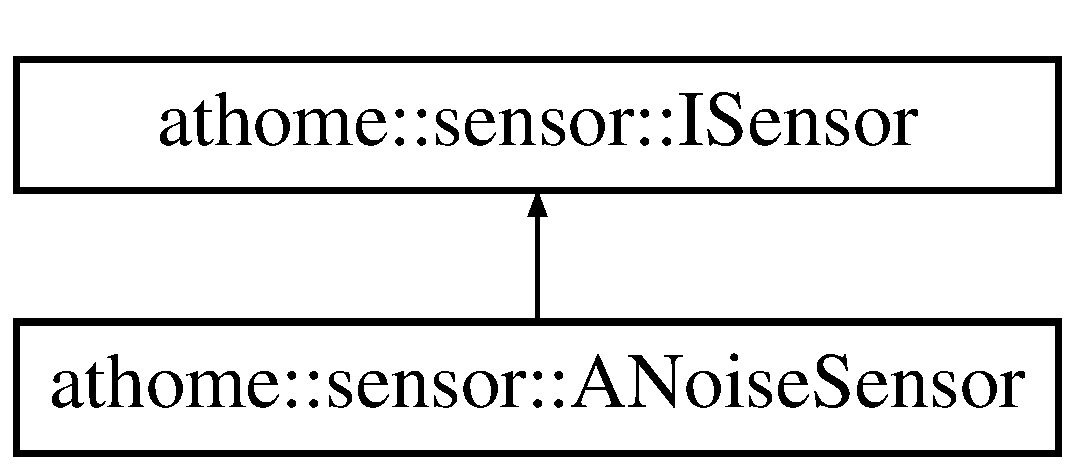
\includegraphics[height=2.000000cm]{classathome_1_1sensor_1_1_a_noise_sensor}
\end{center}
\end{figure}
\subsection*{Public Member Functions}
\begin{DoxyCompactItemize}
\item 
\mbox{\Hypertarget{classathome_1_1sensor_1_1_a_noise_sensor_add13fcd855f63aa6f0a455c341e1d6e1}\label{classathome_1_1sensor_1_1_a_noise_sensor_add13fcd855f63aa6f0a455c341e1d6e1}} 
{\bfseries A\+Noise\+Sensor} (const \mbox{\hyperlink{classathome_1_1sensor_1_1_a_noise_sensor}{A\+Noise\+Sensor}} \&)=delete
\item 
\mbox{\Hypertarget{classathome_1_1sensor_1_1_a_noise_sensor_a44ad4ecd3efe2567dfe7a32ee6aaf8b7}\label{classathome_1_1sensor_1_1_a_noise_sensor_a44ad4ecd3efe2567dfe7a32ee6aaf8b7}} 
\mbox{\hyperlink{classathome_1_1sensor_1_1_a_noise_sensor}{A\+Noise\+Sensor}} \& {\bfseries operator=} (const \mbox{\hyperlink{classathome_1_1sensor_1_1_a_noise_sensor}{A\+Noise\+Sensor}} \&)=delete
\item 
const \mbox{\hyperlink{structathome_1_1sensor_1_1_i_sensor_1_1_i_sensor_value}{I\+Sensor\+Value}} \& \mbox{\hyperlink{classathome_1_1sensor_1_1_a_noise_sensor_ab567b050b41bd0b72fcc9b94b9f6fc6e}{get\+Sample}} ()
\item 
\mbox{\Hypertarget{classathome_1_1sensor_1_1_a_noise_sensor_aad5085d8b0b3ddbf49504af238040ab9}\label{classathome_1_1sensor_1_1_a_noise_sensor_aad5085d8b0b3ddbf49504af238040ab9}} 
virtual int32\+\_\+t {\bfseries get\+Sensor\+Sample} () const =0
\item 
void \mbox{\hyperlink{classathome_1_1sensor_1_1_a_noise_sensor_a8429e91e9f8b2e1634a405780f456beb}{set\+Thresholds}} (const \mbox{\hyperlink{structathome_1_1sensor_1_1_i_sensor_1_1_i_sensor_thresholds}{I\+Sensor\+Thresholds}} \&)
\end{DoxyCompactItemize}
\subsection*{Additional Inherited Members}


\subsection{Member Function Documentation}
\mbox{\Hypertarget{classathome_1_1sensor_1_1_a_noise_sensor_ab567b050b41bd0b72fcc9b94b9f6fc6e}\label{classathome_1_1sensor_1_1_a_noise_sensor_ab567b050b41bd0b72fcc9b94b9f6fc6e}} 
\index{athome\+::sensor\+::\+A\+Noise\+Sensor@{athome\+::sensor\+::\+A\+Noise\+Sensor}!get\+Sample@{get\+Sample}}
\index{get\+Sample@{get\+Sample}!athome\+::sensor\+::\+A\+Noise\+Sensor@{athome\+::sensor\+::\+A\+Noise\+Sensor}}
\subsubsection{\texorpdfstring{get\+Sample()}{getSample()}}
{\footnotesize\ttfamily const \mbox{\hyperlink{structathome_1_1sensor_1_1_i_sensor_1_1_i_sensor_value}{I\+Sensor\+::\+I\+Sensor\+Value}} \& athome\+::sensor\+::\+A\+Noise\+Sensor\+::get\+Sample (\begin{DoxyParamCaption}{ }\end{DoxyParamCaption})\hspace{0.3cm}{\ttfamily [virtual]}}

Returns a pointer on sensor sample raw memory, as an array of bytes 

Implements \mbox{\hyperlink{classathome_1_1sensor_1_1_i_sensor_ae109cd3741ea9c88dc7e4f2eaf1485d5}{athome\+::sensor\+::\+I\+Sensor}}.

\mbox{\Hypertarget{classathome_1_1sensor_1_1_a_noise_sensor_a8429e91e9f8b2e1634a405780f456beb}\label{classathome_1_1sensor_1_1_a_noise_sensor_a8429e91e9f8b2e1634a405780f456beb}} 
\index{athome\+::sensor\+::\+A\+Noise\+Sensor@{athome\+::sensor\+::\+A\+Noise\+Sensor}!set\+Thresholds@{set\+Thresholds}}
\index{set\+Thresholds@{set\+Thresholds}!athome\+::sensor\+::\+A\+Noise\+Sensor@{athome\+::sensor\+::\+A\+Noise\+Sensor}}
\subsubsection{\texorpdfstring{set\+Thresholds()}{setThresholds()}}
{\footnotesize\ttfamily void athome\+::sensor\+::\+A\+Noise\+Sensor\+::set\+Thresholds (\begin{DoxyParamCaption}\item[{const \mbox{\hyperlink{structathome_1_1sensor_1_1_i_sensor_1_1_i_sensor_thresholds}{I\+Sensor\+Thresholds}} \&}]{ }\end{DoxyParamCaption})\hspace{0.3cm}{\ttfamily [virtual]}}

Returns the estimation of safety from the current sensor value

Example\+:


\begin{DoxyCode}
\textcolor{keywordtype}{void} my\_function\_telling\_if\_a\_sensor\_value\_is\_good\_or\_not(ISensor &my\_sensor) \{
  \mbox{\hyperlink{classathome_1_1sensor_1_1_i_sensor_aa70bc27a4c17c86caf96cca776541ddf}{ISensorScale}} sensor\_estimate = my\_sensor.getEstimate();
  \textcolor{keywordflow}{if} (sensor\_estimate == ISensor::ZERO) \{
    Serial.println(\textcolor{stringliteral}{"The sensor returned an invalid value"});
  \}
  \textcolor{keywordflow}{else} \textcolor{keywordflow}{if} (sensor\_estimate > ISensor::ZERO && sensor\_estimate < 6) \{
    Serial.println(\textcolor{stringliteral}{"Boouh, it's not good :("});
  \}
  \textcolor{keywordflow}{else} \{
    Serial.println(\textcolor{stringliteral}{"Yaaaay!"});
  \}
\}
\end{DoxyCode}
 

Implements \mbox{\hyperlink{classathome_1_1sensor_1_1_i_sensor_af86df8538fecfcfc670b4adfbbde6abb}{athome\+::sensor\+::\+I\+Sensor}}.



The documentation for this class was generated from the following files\+:\begin{DoxyCompactItemize}
\item 
src/A\+Noise\+Sensor.\+hpp\item 
src/sensor/sound/A\+Noise\+Sensor.\+cpp\end{DoxyCompactItemize}

\hypertarget{classathome_1_1storage_1_1_arduino_e_e_p_r_o_m}{}\section{athome\+:\+:storage\+:\+:Arduino\+E\+E\+P\+R\+OM Class Reference}
\label{classathome_1_1storage_1_1_arduino_e_e_p_r_o_m}\index{athome\+::storage\+::\+Arduino\+E\+E\+P\+R\+OM@{athome\+::storage\+::\+Arduino\+E\+E\+P\+R\+OM}}


{\ttfamily \#include $<$Arduino\+E\+E\+P\+R\+O\+M.\+hpp$>$}

Inheritance diagram for athome\+:\+:storage\+:\+:Arduino\+E\+E\+P\+R\+OM\+:\begin{figure}[H]
\begin{center}
\leavevmode
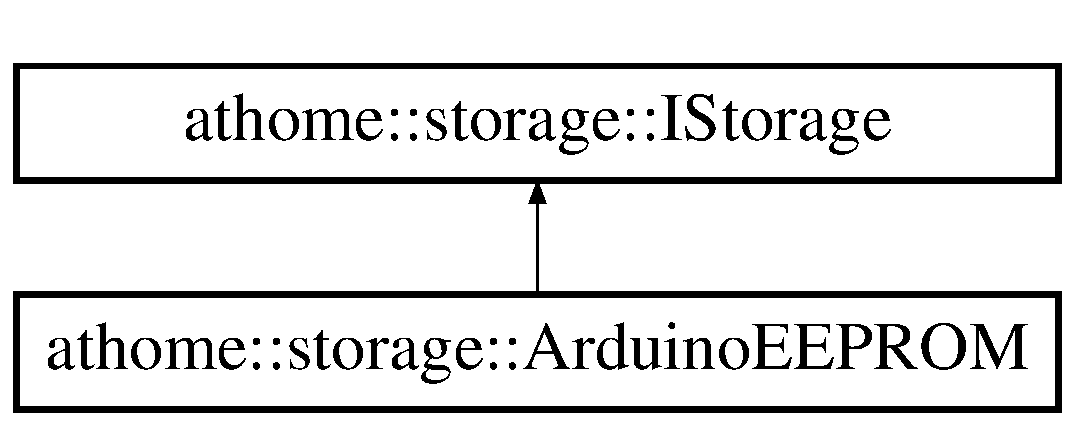
\includegraphics[height=2.000000cm]{classathome_1_1storage_1_1_arduino_e_e_p_r_o_m}
\end{center}
\end{figure}
\subsection*{Public Member Functions}
\begin{DoxyCompactItemize}
\item 
\mbox{\Hypertarget{classathome_1_1storage_1_1_arduino_e_e_p_r_o_m_acd5307c1483893ec3d378299dbf882bf}\label{classathome_1_1storage_1_1_arduino_e_e_p_r_o_m_acd5307c1483893ec3d378299dbf882bf}} 
{\bfseries Arduino\+E\+E\+P\+R\+OM} (const \mbox{\hyperlink{classathome_1_1storage_1_1_arduino_e_e_p_r_o_m}{Arduino\+E\+E\+P\+R\+OM}} \&)=delete
\item 
\mbox{\Hypertarget{classathome_1_1storage_1_1_arduino_e_e_p_r_o_m_a58b6acc1fbf55445a2dbb20879dc4860}\label{classathome_1_1storage_1_1_arduino_e_e_p_r_o_m_a58b6acc1fbf55445a2dbb20879dc4860}} 
\mbox{\hyperlink{classathome_1_1storage_1_1_arduino_e_e_p_r_o_m}{Arduino\+E\+E\+P\+R\+OM}} \& {\bfseries operator=} (const \mbox{\hyperlink{classathome_1_1storage_1_1_arduino_e_e_p_r_o_m}{Arduino\+E\+E\+P\+R\+OM}} \&)=delete
\item 
void \mbox{\hyperlink{classathome_1_1storage_1_1_arduino_e_e_p_r_o_m_a853674189981dd3395ea76911d2eb1a0}{read}} (size\+\_\+t, void $\ast$, size\+\_\+t)
\item 
void \mbox{\hyperlink{classathome_1_1storage_1_1_arduino_e_e_p_r_o_m_a20027ab8a5b20c1fad3e3e42daafe53d}{write}} (size\+\_\+t, const void $\ast$, size\+\_\+t)
\end{DoxyCompactItemize}


\subsection{Detailed Description}
This class is only available on A\+VR platforms using Arduino, as it is a wrapper of Arduino E\+E\+P\+R\+OM library to implement non-\/volatile storage on A\+VR mcu.

Usage is simple, just create an instance of this object and set is as the storage interface of your module using its set\+Storage method\+:


\begin{DoxyCode}
\textcolor{preprocessor}{#include <AtHome.h>}

ArduinoEEPROM eeprom; \textcolor{comment}{// Create an ArduinoEEPROM instance}
AtHomeModule<uint16\_t, 15> *module = AtHomeModule<uint16\_t, 15>::getInstance();

\textcolor{keywordtype}{void} setup() \{
  module->setStorage(&eeprom);
\}

\textcolor{keywordtype}{void} loop() \{
\}
\end{DoxyCode}
 

\subsection{Member Function Documentation}
\mbox{\Hypertarget{classathome_1_1storage_1_1_arduino_e_e_p_r_o_m_a853674189981dd3395ea76911d2eb1a0}\label{classathome_1_1storage_1_1_arduino_e_e_p_r_o_m_a853674189981dd3395ea76911d2eb1a0}} 
\index{athome\+::storage\+::\+Arduino\+E\+E\+P\+R\+OM@{athome\+::storage\+::\+Arduino\+E\+E\+P\+R\+OM}!read@{read}}
\index{read@{read}!athome\+::storage\+::\+Arduino\+E\+E\+P\+R\+OM@{athome\+::storage\+::\+Arduino\+E\+E\+P\+R\+OM}}
\subsubsection{\texorpdfstring{read()}{read()}}
{\footnotesize\ttfamily void athome\+::storage\+::\+Arduino\+E\+E\+P\+R\+O\+M\+::read (\begin{DoxyParamCaption}\item[{size\+\_\+t}]{,  }\item[{void $\ast$}]{,  }\item[{size\+\_\+t}]{ }\end{DoxyParamCaption})\hspace{0.3cm}{\ttfamily [virtual]}}

Copy n bytes (3rd parameter) in dest (2nd parameter) from offset x (1st parameter)

Example\+:


\begin{DoxyCode}
\textcolor{keywordtype}{void} my\_function\_reading\_something(IStorage &storage) \{
  \textcolor{keywordtype}{char} my\_string[33];
  \textcolor{keywordtype}{int} my\_number;

  storage.read(0, my\_string, \textcolor{keyword}{sizeof}(my\_string)); \textcolor{comment}{// Reading a string (array of 33 char) at offset 0 of
       storage instance into my\_string}
  storage.read(\textcolor{keyword}{sizeof}(my\_string), &my\_number, \textcolor{keyword}{sizeof}(my\_number)); \textcolor{comment}{// Reading an integer at offset 33 (after
       content put into my\_string) from storage instance into my\_number}
\}
\end{DoxyCode}
 

Implements \mbox{\hyperlink{classathome_1_1storage_1_1_i_storage_af623393cdf559addf167463ce4e7005e}{athome\+::storage\+::\+I\+Storage}}.

\mbox{\Hypertarget{classathome_1_1storage_1_1_arduino_e_e_p_r_o_m_a20027ab8a5b20c1fad3e3e42daafe53d}\label{classathome_1_1storage_1_1_arduino_e_e_p_r_o_m_a20027ab8a5b20c1fad3e3e42daafe53d}} 
\index{athome\+::storage\+::\+Arduino\+E\+E\+P\+R\+OM@{athome\+::storage\+::\+Arduino\+E\+E\+P\+R\+OM}!write@{write}}
\index{write@{write}!athome\+::storage\+::\+Arduino\+E\+E\+P\+R\+OM@{athome\+::storage\+::\+Arduino\+E\+E\+P\+R\+OM}}
\subsubsection{\texorpdfstring{write()}{write()}}
{\footnotesize\ttfamily void athome\+::storage\+::\+Arduino\+E\+E\+P\+R\+O\+M\+::write (\begin{DoxyParamCaption}\item[{size\+\_\+t}]{,  }\item[{const void $\ast$}]{,  }\item[{size\+\_\+t}]{ }\end{DoxyParamCaption})\hspace{0.3cm}{\ttfamily [virtual]}}

Write n bytes (3rd parameter) in offset x (1st parameter) from src (2nd parameter)

Example\+:


\begin{DoxyCode}
\textcolor{keywordtype}{void} my\_function\_writing\_something(IStorage &storage) \{
  \textcolor{keywordtype}{char} my\_string[] = \textcolor{stringliteral}{"Hello, World!"};
  \textcolor{keywordtype}{int} my\_number = 42;

  storage.write(0, my\_string, \textcolor{keyword}{sizeof}(my\_string)); \textcolor{comment}{// Writing the string (array of 14 char) my\_string at
       offset 0 of storage instance}
  storage.write(\textcolor{keyword}{sizeof}(my\_string), &my\_number, \textcolor{keyword}{sizeof}(my\_number)); \textcolor{comment}{// Writing my\_number at offset 14 (after
       my\_string) of storage instance}
\}
\end{DoxyCode}
 

Implements \mbox{\hyperlink{classathome_1_1storage_1_1_i_storage_a1017bb6ad438313b98197893954e52f1}{athome\+::storage\+::\+I\+Storage}}.



The documentation for this class was generated from the following files\+:\begin{DoxyCompactItemize}
\item 
src/Arduino\+E\+E\+P\+R\+O\+M.\+hpp\item 
src/storage/Arduino\+E\+E\+P\+R\+O\+M.\+cpp\end{DoxyCompactItemize}

\hypertarget{classathome_1_1display_1_1_a_r_g_b_led}{}\section{athome\+:\+:display\+:\+:A\+R\+G\+B\+Led Class Reference}
\label{classathome_1_1display_1_1_a_r_g_b_led}\index{athome\+::display\+::\+A\+R\+G\+B\+Led@{athome\+::display\+::\+A\+R\+G\+B\+Led}}


{\ttfamily \#include $<$A\+R\+G\+B\+Led.\+hpp$>$}

Inheritance diagram for athome\+:\+:display\+:\+:A\+R\+G\+B\+Led\+:\begin{figure}[H]
\begin{center}
\leavevmode
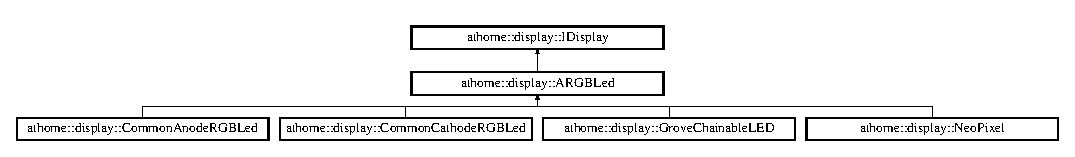
\includegraphics[height=2.213439cm]{classathome_1_1display_1_1_a_r_g_b_led}
\end{center}
\end{figure}
\subsection*{Classes}
\begin{DoxyCompactItemize}
\item 
struct \mbox{\hyperlink{structathome_1_1display_1_1_a_r_g_b_led_1_1_color}{Color}}
\end{DoxyCompactItemize}
\subsection*{Public Member Functions}
\begin{DoxyCompactItemize}
\item 
\mbox{\Hypertarget{classathome_1_1display_1_1_a_r_g_b_led_ac4556a22050f3a1beff3134977f72589}\label{classathome_1_1display_1_1_a_r_g_b_led_ac4556a22050f3a1beff3134977f72589}} 
{\bfseries A\+R\+G\+B\+Led} (\mbox{\hyperlink{classathome_1_1display_1_1_a_r_g_b_led}{A\+R\+G\+B\+Led}} const \&)=delete
\item 
\mbox{\Hypertarget{classathome_1_1display_1_1_a_r_g_b_led_a8ff479add175bb3a99426301c2db87ce}\label{classathome_1_1display_1_1_a_r_g_b_led_a8ff479add175bb3a99426301c2db87ce}} 
\mbox{\hyperlink{classathome_1_1display_1_1_a_r_g_b_led}{A\+R\+G\+B\+Led}} \& {\bfseries operator=} (\mbox{\hyperlink{classathome_1_1display_1_1_a_r_g_b_led}{A\+R\+G\+B\+Led}} const \&)=delete
\item 
void \mbox{\hyperlink{classathome_1_1display_1_1_a_r_g_b_led_a9753e3a23ea5cb6b0a41079bc6128766}{clear}} ()
\item 
virtual void \mbox{\hyperlink{classathome_1_1display_1_1_a_r_g_b_led_a725ceca0c01735daa9c95148baf075ab}{update}} ()=0
\item 
const \mbox{\hyperlink{structathome_1_1display_1_1_a_r_g_b_led_1_1_color}{Color}} \& \mbox{\hyperlink{classathome_1_1display_1_1_a_r_g_b_led_a2c3022a5aad43595fefc4b52d916467a}{get\+Color}} () const
\item 
void \mbox{\hyperlink{classathome_1_1display_1_1_a_r_g_b_led_a7ca4858c1ee10cc2f7c1dcc11a6d050e}{set\+Color}} (const \mbox{\hyperlink{structathome_1_1display_1_1_a_r_g_b_led_1_1_color}{Color}} \&color)
\item 
virtual void \mbox{\hyperlink{classathome_1_1display_1_1_a_r_g_b_led_a1e6a934912f71a5ea06df1d28cf5ace9}{set\+Displayed\+Estimate}} (\mbox{\hyperlink{classathome_1_1sensor_1_1_i_sensor_aa70bc27a4c17c86caf96cca776541ddf}{sensor\+::\+I\+Sensor\+::\+I\+Sensor\+Scale}} value)
\item 
void \mbox{\hyperlink{classathome_1_1display_1_1_a_r_g_b_led_a411b35199d593b813bad7d9056678198}{set\+Colors\+Scale}} (const \mbox{\hyperlink{structathome_1_1display_1_1_a_r_g_b_led_1_1_color}{Color}} scale\mbox{[}$\,$\mbox{]})
\item 
void \mbox{\hyperlink{classathome_1_1display_1_1_a_r_g_b_led_a69e31887e1a37a86073d5f82bd578f1f}{set\+Individual\+Color\+Scale}} (const \mbox{\hyperlink{structathome_1_1display_1_1_a_r_g_b_led_1_1_color}{Color}} \&color, \mbox{\hyperlink{classathome_1_1sensor_1_1_i_sensor_aa70bc27a4c17c86caf96cca776541ddf}{sensor\+::\+I\+Sensor\+::\+I\+Sensor\+Scale}} value)
\end{DoxyCompactItemize}


\subsection{Detailed Description}
Abstract class used to control R\+GB L\+E\+Ds (Common cathode/anode, Grove Chainable L\+E\+Ds, Neo\+Pixels, ...etc)

Example of use\+:


\begin{DoxyCode}
\textcolor{keywordtype}{void} my\_function\_changing\_led\_color(ARGBLed &led) \{
  Color red = \{255, 0, 0\}; \textcolor{comment}{// Create a Color structure with red fully on,}
green off and blue off led.setColor(red); \textcolor{comment}{// Set the new color by calling}
\mbox{\hyperlink{classathome_1_1display_1_1_a_r_g_b_led_a7ca4858c1ee10cc2f7c1dcc11a6d050e}{setColor}} method led.update(); \textcolor{comment}{// Display the new color on the LED}
\}
\end{DoxyCode}
 

\subsection{Member Function Documentation}
\mbox{\Hypertarget{classathome_1_1display_1_1_a_r_g_b_led_a9753e3a23ea5cb6b0a41079bc6128766}\label{classathome_1_1display_1_1_a_r_g_b_led_a9753e3a23ea5cb6b0a41079bc6128766}} 
\index{athome\+::display\+::\+A\+R\+G\+B\+Led@{athome\+::display\+::\+A\+R\+G\+B\+Led}!clear@{clear}}
\index{clear@{clear}!athome\+::display\+::\+A\+R\+G\+B\+Led@{athome\+::display\+::\+A\+R\+G\+B\+Led}}
\subsubsection{\texorpdfstring{clear()}{clear()}}
{\footnotesize\ttfamily void athome\+::display\+::\+A\+R\+G\+B\+Led\+::clear (\begin{DoxyParamCaption}{ }\end{DoxyParamCaption})\hspace{0.3cm}{\ttfamily [inline]}, {\ttfamily [virtual]}}

Remove display content 

Implements \mbox{\hyperlink{classathome_1_1display_1_1_i_display_a0d3add1ce61c96657827fb56d250d9c6}{athome\+::display\+::\+I\+Display}}.

\mbox{\Hypertarget{classathome_1_1display_1_1_a_r_g_b_led_a2c3022a5aad43595fefc4b52d916467a}\label{classathome_1_1display_1_1_a_r_g_b_led_a2c3022a5aad43595fefc4b52d916467a}} 
\index{athome\+::display\+::\+A\+R\+G\+B\+Led@{athome\+::display\+::\+A\+R\+G\+B\+Led}!get\+Color@{get\+Color}}
\index{get\+Color@{get\+Color}!athome\+::display\+::\+A\+R\+G\+B\+Led@{athome\+::display\+::\+A\+R\+G\+B\+Led}}
\subsubsection{\texorpdfstring{get\+Color()}{getColor()}}
{\footnotesize\ttfamily const \mbox{\hyperlink{structathome_1_1display_1_1_a_r_g_b_led_1_1_color}{Color}}\& athome\+::display\+::\+A\+R\+G\+B\+Led\+::get\+Color (\begin{DoxyParamCaption}{ }\end{DoxyParamCaption}) const\hspace{0.3cm}{\ttfamily [inline]}}

Return a reference on the \mbox{\hyperlink{structathome_1_1display_1_1_a_r_g_b_led_1_1_color}{Color}} structure representing the current color displayed (or next color, if L\+ED color hasn\textquotesingle{}t been updated since last change of color made by set\+Color)

Example\+:


\begin{DoxyCode}
\textcolor{keywordtype}{void} my\_function\_printing\_led\_color(\textcolor{keyword}{const} ARGBLed &led) \{
  \textcolor{keyword}{const} Color &color = led.getColor();
\textcolor{preprocessor}{#ifdef ARDUINO}
  Serial.print(\textcolor{stringliteral}{"Red: "});
  Serial.print(led.red);
  Serial.print(\textcolor{stringliteral}{", Green: "});
  Serial.print(led.green);
  Serial.print(\textcolor{stringliteral}{", Blue: "});
  Serial.println(led.blue);
\textcolor{preprocessor}{#else}
  printf(\textcolor{stringliteral}{"Red: %u, Green: %u, Blue: %u\(\backslash\)n"}, led.red, led.green, led.blue);
\textcolor{preprocessor}{#endif}
\textcolor{preprocessor}{\}}
\end{DoxyCode}
 \mbox{\Hypertarget{classathome_1_1display_1_1_a_r_g_b_led_a7ca4858c1ee10cc2f7c1dcc11a6d050e}\label{classathome_1_1display_1_1_a_r_g_b_led_a7ca4858c1ee10cc2f7c1dcc11a6d050e}} 
\index{athome\+::display\+::\+A\+R\+G\+B\+Led@{athome\+::display\+::\+A\+R\+G\+B\+Led}!set\+Color@{set\+Color}}
\index{set\+Color@{set\+Color}!athome\+::display\+::\+A\+R\+G\+B\+Led@{athome\+::display\+::\+A\+R\+G\+B\+Led}}
\subsubsection{\texorpdfstring{set\+Color()}{setColor()}}
{\footnotesize\ttfamily void athome\+::display\+::\+A\+R\+G\+B\+Led\+::set\+Color (\begin{DoxyParamCaption}\item[{const \mbox{\hyperlink{structathome_1_1display_1_1_a_r_g_b_led_1_1_color}{Color}} \&}]{color }\end{DoxyParamCaption})\hspace{0.3cm}{\ttfamily [inline]}}

Set the new color to display on the L\+ED.

Note\+: You need to call the \char`\"{}update\char`\"{} method after this one, as it doesn\textquotesingle{}t update automatically the new color on the L\+ED.

Example\+:


\begin{DoxyCode}
\textcolor{keyword}{const} Color red = \{255, 0, 0\};

\textcolor{keywordtype}{void} my\_function\_changing\_a\_led\_color\_to\_red(ARGBLed &led) \{
  led.setColor(red); \textcolor{comment}{// Set the new color in the LED object}
  led.update(); \textcolor{comment}{// You need to call this method if you want the new color}
to be displayed on the LED
\}
\end{DoxyCode}
 \mbox{\Hypertarget{classathome_1_1display_1_1_a_r_g_b_led_a411b35199d593b813bad7d9056678198}\label{classathome_1_1display_1_1_a_r_g_b_led_a411b35199d593b813bad7d9056678198}} 
\index{athome\+::display\+::\+A\+R\+G\+B\+Led@{athome\+::display\+::\+A\+R\+G\+B\+Led}!set\+Colors\+Scale@{set\+Colors\+Scale}}
\index{set\+Colors\+Scale@{set\+Colors\+Scale}!athome\+::display\+::\+A\+R\+G\+B\+Led@{athome\+::display\+::\+A\+R\+G\+B\+Led}}
\subsubsection{\texorpdfstring{set\+Colors\+Scale()}{setColorsScale()}}
{\footnotesize\ttfamily void athome\+::display\+::\+A\+R\+G\+B\+Led\+::set\+Colors\+Scale (\begin{DoxyParamCaption}\item[{const \mbox{\hyperlink{structathome_1_1display_1_1_a_r_g_b_led_1_1_color}{Color}}}]{scale\mbox{[}$\,$\mbox{]} }\end{DoxyParamCaption})\hspace{0.3cm}{\ttfamily [inline]}}

Change the scale of colors associated to each values of I\+Sensor\+Scale by passing an array containing all colors as a parameter \mbox{\Hypertarget{classathome_1_1display_1_1_a_r_g_b_led_a1e6a934912f71a5ea06df1d28cf5ace9}\label{classathome_1_1display_1_1_a_r_g_b_led_a1e6a934912f71a5ea06df1d28cf5ace9}} 
\index{athome\+::display\+::\+A\+R\+G\+B\+Led@{athome\+::display\+::\+A\+R\+G\+B\+Led}!set\+Displayed\+Estimate@{set\+Displayed\+Estimate}}
\index{set\+Displayed\+Estimate@{set\+Displayed\+Estimate}!athome\+::display\+::\+A\+R\+G\+B\+Led@{athome\+::display\+::\+A\+R\+G\+B\+Led}}
\subsubsection{\texorpdfstring{set\+Displayed\+Estimate()}{setDisplayedEstimate()}}
{\footnotesize\ttfamily virtual void athome\+::display\+::\+A\+R\+G\+B\+Led\+::set\+Displayed\+Estimate (\begin{DoxyParamCaption}\item[{\mbox{\hyperlink{classathome_1_1sensor_1_1_i_sensor_aa70bc27a4c17c86caf96cca776541ddf}{sensor\+::\+I\+Sensor\+::\+I\+Sensor\+Scale}}}]{ }\end{DoxyParamCaption})\hspace{0.3cm}{\ttfamily [inline]}, {\ttfamily [virtual]}}

Set the value displayed on the screen, whatever the type of display is.

I\+Sensor\+Scale is an enumeration representing the correctness on a scale from 1 to 10 (1 is worst, 10 is best).

This scale can be represented by various ways for many different displays. For example\+:


\begin{DoxyItemize}
\item An L\+ED could stay off from 6 and on below 6
\item A dimmable L\+ED could set it\textquotesingle{}s percentage of brightness corresponding to the value (for example 1 = 100\%, 5 = 50\%, 10 = 0\%)
\item A 7 segments display could display the digit itself and stay off at 10
\item An L\+CD screen could write a sentence, the digit, draw a gauge, ...etc
\item A speaker or buzzer could do noise of different intensities below 6
\item ...etc 
\end{DoxyItemize}

Implements \mbox{\hyperlink{classathome_1_1display_1_1_i_display_a3c9678f929e4bc04742d458b0c2399ef}{athome\+::display\+::\+I\+Display}}.

\mbox{\Hypertarget{classathome_1_1display_1_1_a_r_g_b_led_a69e31887e1a37a86073d5f82bd578f1f}\label{classathome_1_1display_1_1_a_r_g_b_led_a69e31887e1a37a86073d5f82bd578f1f}} 
\index{athome\+::display\+::\+A\+R\+G\+B\+Led@{athome\+::display\+::\+A\+R\+G\+B\+Led}!set\+Individual\+Color\+Scale@{set\+Individual\+Color\+Scale}}
\index{set\+Individual\+Color\+Scale@{set\+Individual\+Color\+Scale}!athome\+::display\+::\+A\+R\+G\+B\+Led@{athome\+::display\+::\+A\+R\+G\+B\+Led}}
\subsubsection{\texorpdfstring{set\+Individual\+Color\+Scale()}{setIndividualColorScale()}}
{\footnotesize\ttfamily void athome\+::display\+::\+A\+R\+G\+B\+Led\+::set\+Individual\+Color\+Scale (\begin{DoxyParamCaption}\item[{const \mbox{\hyperlink{structathome_1_1display_1_1_a_r_g_b_led_1_1_color}{Color}} \&}]{color,  }\item[{\mbox{\hyperlink{classathome_1_1sensor_1_1_i_sensor_aa70bc27a4c17c86caf96cca776541ddf}{sensor\+::\+I\+Sensor\+::\+I\+Sensor\+Scale}}}]{value }\end{DoxyParamCaption})\hspace{0.3cm}{\ttfamily [inline]}}

Change the color associated to a certain value of the scale I\+Sensor\+Scale \mbox{\Hypertarget{classathome_1_1display_1_1_a_r_g_b_led_a725ceca0c01735daa9c95148baf075ab}\label{classathome_1_1display_1_1_a_r_g_b_led_a725ceca0c01735daa9c95148baf075ab}} 
\index{athome\+::display\+::\+A\+R\+G\+B\+Led@{athome\+::display\+::\+A\+R\+G\+B\+Led}!update@{update}}
\index{update@{update}!athome\+::display\+::\+A\+R\+G\+B\+Led@{athome\+::display\+::\+A\+R\+G\+B\+Led}}
\subsubsection{\texorpdfstring{update()}{update()}}
{\footnotesize\ttfamily virtual void athome\+::display\+::\+A\+R\+G\+B\+Led\+::update (\begin{DoxyParamCaption}{ }\end{DoxyParamCaption})\hspace{0.3cm}{\ttfamily [pure virtual]}}

Update display content 

Implements \mbox{\hyperlink{classathome_1_1display_1_1_i_display_a4ba7bd5d46f88578f1c846f4f5f3c5d1}{athome\+::display\+::\+I\+Display}}.



Implemented in \mbox{\hyperlink{classathome_1_1display_1_1_grove_chainable_l_e_d_a05a4a1381396b7fc11a24993865d8226}{athome\+::display\+::\+Grove\+Chainable\+L\+ED}}, \mbox{\hyperlink{classathome_1_1display_1_1_common_anode_r_g_b_led_ab7daf7dcc6ac1e3fcab202cae484b237}{athome\+::display\+::\+Common\+Anode\+R\+G\+B\+Led}}, and \mbox{\hyperlink{classathome_1_1display_1_1_common_cathode_r_g_b_led_ab78ab6aef619d8e0941dd11d4cfbb545}{athome\+::display\+::\+Common\+Cathode\+R\+G\+B\+Led}}.



The documentation for this class was generated from the following file\+:\begin{DoxyCompactItemize}
\item 
src/A\+R\+G\+B\+Led.\+hpp\end{DoxyCompactItemize}

\hypertarget{classathome_1_1sensor_1_1_a_temperature_sensor}{}\section{athome\+:\+:sensor\+:\+:A\+Temperature\+Sensor Class Reference}
\label{classathome_1_1sensor_1_1_a_temperature_sensor}\index{athome\+::sensor\+::\+A\+Temperature\+Sensor@{athome\+::sensor\+::\+A\+Temperature\+Sensor}}
Inheritance diagram for athome\+:\+:sensor\+:\+:A\+Temperature\+Sensor\+:\begin{figure}[H]
\begin{center}
\leavevmode
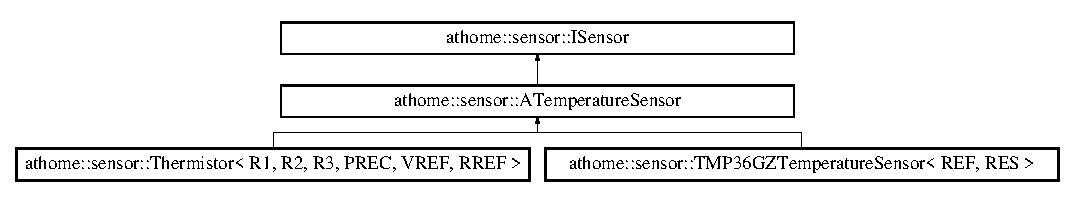
\includegraphics[height=2.204725cm]{classathome_1_1sensor_1_1_a_temperature_sensor}
\end{center}
\end{figure}
\subsection*{Public Member Functions}
\begin{DoxyCompactItemize}
\item 
\mbox{\Hypertarget{classathome_1_1sensor_1_1_a_temperature_sensor_adc643a183aa4e4ae6b6c8c9212aa6525}\label{classathome_1_1sensor_1_1_a_temperature_sensor_adc643a183aa4e4ae6b6c8c9212aa6525}} 
{\bfseries A\+Temperature\+Sensor} (const \mbox{\hyperlink{classathome_1_1sensor_1_1_a_temperature_sensor}{A\+Temperature\+Sensor}} \&)=delete
\item 
\mbox{\Hypertarget{classathome_1_1sensor_1_1_a_temperature_sensor_a0eb5857e7a283d824b183eb55239e9fe}\label{classathome_1_1sensor_1_1_a_temperature_sensor_a0eb5857e7a283d824b183eb55239e9fe}} 
\mbox{\hyperlink{classathome_1_1sensor_1_1_a_temperature_sensor}{A\+Temperature\+Sensor}} \& {\bfseries operator=} (const \mbox{\hyperlink{classathome_1_1sensor_1_1_a_temperature_sensor}{A\+Temperature\+Sensor}} \&)=delete
\item 
virtual const \mbox{\hyperlink{structathome_1_1sensor_1_1_i_sensor_1_1_i_sensor_value}{I\+Sensor\+Value}} \& \mbox{\hyperlink{classathome_1_1sensor_1_1_a_temperature_sensor_afea6a461b8dff9ee736aa508aa4f6a3c}{get\+Sample}} ()
\item 
virtual int32\+\_\+t \mbox{\hyperlink{classathome_1_1sensor_1_1_a_temperature_sensor_a4e5b2c79ab69f6903f7b322da45b0af4}{get\+Sensor\+Sample}} ()=0
\item 
virtual void \mbox{\hyperlink{classathome_1_1sensor_1_1_a_temperature_sensor_a1c323184ac116784e877151895dfd080}{set\+Thresholds}} (const \mbox{\hyperlink{structathome_1_1sensor_1_1_i_sensor_1_1_i_sensor_thresholds}{I\+Sensor\+Thresholds}} \&)
\end{DoxyCompactItemize}
\subsection*{Additional Inherited Members}


\subsection{Member Function Documentation}
\mbox{\Hypertarget{classathome_1_1sensor_1_1_a_temperature_sensor_afea6a461b8dff9ee736aa508aa4f6a3c}\label{classathome_1_1sensor_1_1_a_temperature_sensor_afea6a461b8dff9ee736aa508aa4f6a3c}} 
\index{athome\+::sensor\+::\+A\+Temperature\+Sensor@{athome\+::sensor\+::\+A\+Temperature\+Sensor}!get\+Sample@{get\+Sample}}
\index{get\+Sample@{get\+Sample}!athome\+::sensor\+::\+A\+Temperature\+Sensor@{athome\+::sensor\+::\+A\+Temperature\+Sensor}}
\subsubsection{\texorpdfstring{get\+Sample()}{getSample()}}
{\footnotesize\ttfamily const \mbox{\hyperlink{structathome_1_1sensor_1_1_i_sensor_1_1_i_sensor_value}{I\+Sensor\+::\+I\+Sensor\+Value}} \& athome\+::sensor\+::\+A\+Temperature\+Sensor\+::get\+Sample (\begin{DoxyParamCaption}{ }\end{DoxyParamCaption})\hspace{0.3cm}{\ttfamily [virtual]}}

Returns a pointer on the sample of the sensor. This pointer needs to point on a float variable.

Return an estimation of the quality of the temperature

Values are from\+: \href{https://www.jechange.fr/energie/duale/guides/thermostat-temperature-4101}{\tt https\+://www.\+jechange.\+fr/energie/duale/guides/thermostat-\/temperature-\/4101} \begin{DoxyReturn}{Returns}
estimation of temperature on a scale from 1 (worst) to 10 (best) 
\end{DoxyReturn}


Implements \mbox{\hyperlink{classathome_1_1sensor_1_1_i_sensor_ae109cd3741ea9c88dc7e4f2eaf1485d5}{athome\+::sensor\+::\+I\+Sensor}}.

\mbox{\Hypertarget{classathome_1_1sensor_1_1_a_temperature_sensor_a4e5b2c79ab69f6903f7b322da45b0af4}\label{classathome_1_1sensor_1_1_a_temperature_sensor_a4e5b2c79ab69f6903f7b322da45b0af4}} 
\index{athome\+::sensor\+::\+A\+Temperature\+Sensor@{athome\+::sensor\+::\+A\+Temperature\+Sensor}!get\+Sensor\+Sample@{get\+Sensor\+Sample}}
\index{get\+Sensor\+Sample@{get\+Sensor\+Sample}!athome\+::sensor\+::\+A\+Temperature\+Sensor@{athome\+::sensor\+::\+A\+Temperature\+Sensor}}
\subsubsection{\texorpdfstring{get\+Sensor\+Sample()}{getSensorSample()}}
{\footnotesize\ttfamily virtual int32\+\_\+t athome\+::sensor\+::\+A\+Temperature\+Sensor\+::get\+Sensor\+Sample (\begin{DoxyParamCaption}{ }\end{DoxyParamCaption})\hspace{0.3cm}{\ttfamily [pure virtual]}}

Returns the last value sampled from the sensor (do not actually resample it). 

Implemented in \mbox{\hyperlink{classathome_1_1sensor_1_1_thermistor_abc45d8d277fb186b5d303f9e53bf73d4}{athome\+::sensor\+::\+Thermistor$<$ R1, R2, R3, P\+R\+E\+C, V\+R\+E\+F, R\+R\+E\+F $>$}}, and \mbox{\hyperlink{classathome_1_1sensor_1_1_t_m_p36_g_z_temperature_sensor_ae0e101ee54c5c64842d2cab9fb9292f4}{athome\+::sensor\+::\+T\+M\+P36\+G\+Z\+Temperature\+Sensor$<$ R\+E\+F, R\+E\+S $>$}}.

\mbox{\Hypertarget{classathome_1_1sensor_1_1_a_temperature_sensor_a1c323184ac116784e877151895dfd080}\label{classathome_1_1sensor_1_1_a_temperature_sensor_a1c323184ac116784e877151895dfd080}} 
\index{athome\+::sensor\+::\+A\+Temperature\+Sensor@{athome\+::sensor\+::\+A\+Temperature\+Sensor}!set\+Thresholds@{set\+Thresholds}}
\index{set\+Thresholds@{set\+Thresholds}!athome\+::sensor\+::\+A\+Temperature\+Sensor@{athome\+::sensor\+::\+A\+Temperature\+Sensor}}
\subsubsection{\texorpdfstring{set\+Thresholds()}{setThresholds()}}
{\footnotesize\ttfamily void athome\+::sensor\+::\+A\+Temperature\+Sensor\+::set\+Thresholds (\begin{DoxyParamCaption}\item[{const \mbox{\hyperlink{structathome_1_1sensor_1_1_i_sensor_1_1_i_sensor_thresholds}{I\+Sensor\+Thresholds}} \&}]{ }\end{DoxyParamCaption})\hspace{0.3cm}{\ttfamily [virtual]}}

Returns the estimation of safety from the current sensor value

Example\+:


\begin{DoxyCode}
\textcolor{keywordtype}{void} my\_function\_telling\_if\_a\_sensor\_value\_is\_good\_or\_not(ISensor &my\_sensor) \{
  \mbox{\hyperlink{classathome_1_1sensor_1_1_i_sensor_aa70bc27a4c17c86caf96cca776541ddf}{ISensorScale}} sensor\_estimate = my\_sensor.getEstimate();
  \textcolor{keywordflow}{if} (sensor\_estimate == ISensor::ZERO) \{
    Serial.println(\textcolor{stringliteral}{"The sensor returned an invalid value"});
  \}
  \textcolor{keywordflow}{else} \textcolor{keywordflow}{if} (sensor\_estimate > ISensor::ZERO && sensor\_estimate < 6) \{
    Serial.println(\textcolor{stringliteral}{"Boouh, it's not good :("});
  \}
  \textcolor{keywordflow}{else} \{
    Serial.println(\textcolor{stringliteral}{"Yaaaay!"});
  \}
\}
\end{DoxyCode}
 

Implements \mbox{\hyperlink{classathome_1_1sensor_1_1_i_sensor_af86df8538fecfcfc670b4adfbbde6abb}{athome\+::sensor\+::\+I\+Sensor}}.



The documentation for this class was generated from the following files\+:\begin{DoxyCompactItemize}
\item 
src/A\+Temperature\+Sensor.\+hpp\item 
src/sensor/temperature/A\+Temperature\+Sensor.\+cpp\end{DoxyCompactItemize}

\hypertarget{classathome_1_1module_1_1_at_home_module}{}\section{athome\+:\+:module\+:\+:At\+Home\+Module$<$ T, n $>$ Class Template Reference}
\label{classathome_1_1module_1_1_at_home_module}\index{athome\+::module\+::\+At\+Home\+Module$<$ T, n $>$@{athome\+::module\+::\+At\+Home\+Module$<$ T, n $>$}}


{\ttfamily \#include $<$At\+Home\+Module.\+hpp$>$}

Inheritance diagram for athome\+:\+:module\+:\+:At\+Home\+Module$<$ T, n $>$\+:\begin{figure}[H]
\begin{center}
\leavevmode
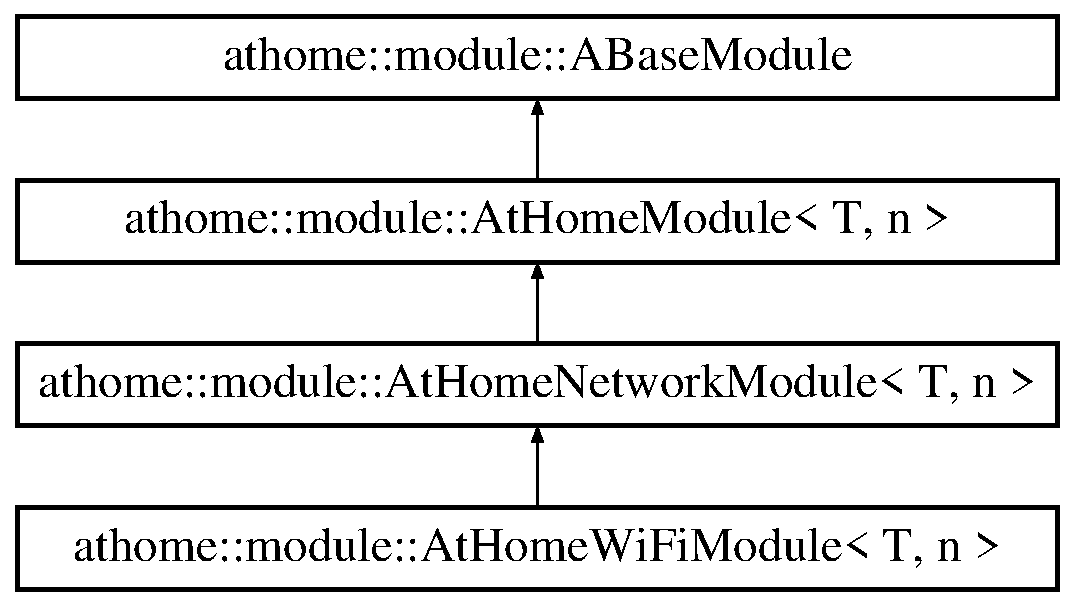
\includegraphics[height=4.000000cm]{classathome_1_1module_1_1_at_home_module}
\end{center}
\end{figure}
\subsection*{Classes}
\begin{DoxyCompactItemize}
\item 
struct \mbox{\hyperlink{structathome_1_1module_1_1_at_home_module_1_1_at_home_sensor_measure}{At\+Home\+Sensor\+Measure}}
\end{DoxyCompactItemize}
\subsection*{Public Types}
\begin{DoxyCompactItemize}
\item 
typedef uint32\+\_\+t \mbox{\hyperlink{classathome_1_1module_1_1_at_home_module_aaa31c8eddb689010ef59deba4e1463c6}{module\+Serial}}
\item 
typedef \mbox{\hyperlink{structathome_1_1time_1_1_i_time_1_1_i_s_o8601_date_time}{time\+::\+I\+Time\+::\+I\+S\+O8601\+Date\+Time}} \mbox{\hyperlink{classathome_1_1module_1_1_at_home_module_a077afdad789e433d59c588ec6c0f4594}{t\+\_\+timestamp}}
\item 
\mbox{\Hypertarget{classathome_1_1module_1_1_at_home_module_a4ae49e9e7d0e5f4e9f9148ef76a288dd}\label{classathome_1_1module_1_1_at_home_module_a4ae49e9e7d0e5f4e9f9148ef76a288dd}} 
typedef void($\ast$ {\bfseries custom\+Callback}) ()
\item 
\mbox{\Hypertarget{classathome_1_1module_1_1_at_home_module_a46fbde0e1376feef862e5cf5ca7b2570}\label{classathome_1_1module_1_1_at_home_module_a46fbde0e1376feef862e5cf5ca7b2570}} 
typedef void($\ast$ {\bfseries At\+Home\+Command\+Plugin}) (const String \&, Stream \&)
\item 
\mbox{\Hypertarget{classathome_1_1module_1_1_at_home_module_a5c269b52c37b8ad6cb73f1607aecb0db}\label{classathome_1_1module_1_1_at_home_module_a5c269b52c37b8ad6cb73f1607aecb0db}} 
typedef void($\ast$ {\bfseries At\+Home\+Storage\+Plugin}) (size\+\_\+t, \mbox{\hyperlink{classathome_1_1storage_1_1_i_storage}{storage\+::\+I\+Storage}} \&)
\end{DoxyCompactItemize}
\subsection*{Public Member Functions}
\begin{DoxyCompactItemize}
\item 
\mbox{\hyperlink{classathome_1_1module_1_1_at_home_module_ad78045943a579874ec16e14cf976eada}{At\+Home\+Module}} (const \mbox{\hyperlink{classathome_1_1module_1_1_at_home_module}{At\+Home\+Module}} \&)=delete
\item 
\mbox{\hyperlink{classathome_1_1module_1_1_at_home_module}{At\+Home\+Module}} \& \mbox{\hyperlink{classathome_1_1module_1_1_at_home_module_aec07a48057f5d52c9adaea375a6a7ad4}{operator=}} (const \mbox{\hyperlink{classathome_1_1module_1_1_at_home_module}{At\+Home\+Module}} \&)=delete
\item 
Scheduler \& \mbox{\hyperlink{classathome_1_1module_1_1_at_home_module_a954f37f05e5738f270a35fef58782ba6}{get\+Scheduler}} ()
\item 
void \mbox{\hyperlink{classathome_1_1module_1_1_at_home_module_a5354c736954a788c51e7cf25f6ccf89d}{setup}} ()
\item 
void \mbox{\hyperlink{classathome_1_1module_1_1_at_home_module_ac39915bf4a255e3610515bc18af3029d}{run}} ()
\item 
void \mbox{\hyperlink{classathome_1_1module_1_1_at_home_module_a5589c1eb7edd2ab45d0a3de7bb475bbe}{stop}} ()
\item 
void \mbox{\hyperlink{classathome_1_1module_1_1_at_home_module_a9a3b04d8f83ecbe0e8e368b697449326}{set\+Sensor\+Execution\+Interval}} (unsigned long ms)
\item 
unsigned long \mbox{\hyperlink{classathome_1_1module_1_1_at_home_module_ae0d4458da2bafd104386671d300fb562}{get\+Sensor\+Execution\+Interval}} () const
\item 
virtual void \mbox{\hyperlink{classathome_1_1module_1_1_at_home_module_af1466a92bf4e3d0dc45adff11d8ee5fd}{set\+Sensor\+Execution\+Callback}} (custom\+Callback f=nullptr)
\item 
void \mbox{\hyperlink{classathome_1_1module_1_1_at_home_module_ad28a042bd9f793d9dbd944ec4f76156b}{set\+Communication\+Execution\+Interval}} (unsigned long ms)
\item 
void \mbox{\hyperlink{classathome_1_1module_1_1_at_home_module_aa02b94ab5009d59d337144db364053a6}{set\+Upload\+Data\+Execution\+Interval}} (unsigned long ms)
\item 
unsigned long \mbox{\hyperlink{classathome_1_1module_1_1_at_home_module_a6186e04da0e46cf463d24947538380bb}{get\+Upload\+Data\+Execution\+Interval}} () const
\item 
virtual void \mbox{\hyperlink{classathome_1_1module_1_1_at_home_module_ae27ce52a7171a2cf3a78c5d8f70c2d1d}{set\+Upload\+Data\+Execution\+Callback}} (custom\+Callback f=nullptr)
\item 
unsigned long \mbox{\hyperlink{classathome_1_1module_1_1_at_home_module_a263fe0bea2fa480b3885fee07e2a8221}{get\+Communication\+Execution\+Interval}} () const
\item 
virtual void \mbox{\hyperlink{classathome_1_1module_1_1_at_home_module_a2a89b7e4cd63739b2c48ffbe3bbaf9be}{set\+Communication\+Execution\+Callback}} (custom\+Callback f=nullptr)
\item 
virtual void \mbox{\hyperlink{classathome_1_1module_1_1_at_home_module_a137cdd3cfb9bad5e8e65eddac89ddd41}{set\+Command\+Plugin}} (At\+Home\+Command\+Plugin plugin)
\item 
virtual void \mbox{\hyperlink{classathome_1_1module_1_1_at_home_module_aeb8a36ce4009ad6a578f41cd654877fa}{set\+On\+Backup\+Plugin}} (At\+Home\+Storage\+Plugin plugin)
\item 
virtual void \mbox{\hyperlink{classathome_1_1module_1_1_at_home_module_a7ae30173c9c2871cd374d5d6786f43f6}{set\+On\+Restore\+Plugin}} (At\+Home\+Storage\+Plugin plugin)
\item 
const \mbox{\hyperlink{classathome_1_1module_1_1_at_home_module_aaa31c8eddb689010ef59deba4e1463c6}{module\+Serial}} \mbox{\hyperlink{classathome_1_1module_1_1_at_home_module_a1267bc33e38b25ba52bceddc60ea7df1}{get\+Serial}} () const
\item 
void \mbox{\hyperlink{classathome_1_1module_1_1_at_home_module_a053f38453530fd881376ed1596a14e09}{set\+Serial}} (\mbox{\hyperlink{classathome_1_1module_1_1_at_home_module_aaa31c8eddb689010ef59deba4e1463c6}{module\+Serial}} serial)
\end{DoxyCompactItemize}
\subsection*{Static Public Member Functions}
\begin{DoxyCompactItemize}
\item 
{\footnotesize template$<$typename U  = At\+Home\+Module$>$ }\\static U $\ast$ \mbox{\hyperlink{classathome_1_1module_1_1_at_home_module_acc6e7fc0d86f11648fd81729484e546f}{get\+Instance}} ()
\end{DoxyCompactItemize}
\subsection*{Protected Member Functions}
\begin{DoxyCompactItemize}
\item 
{\footnotesize template$<$typename U $>$ }\\void \mbox{\hyperlink{classathome_1_1module_1_1_at_home_module_a22f6afbe9594849ecccae5b9f4dfe47d}{broadcast}} (const U \&data)
\item 
{\footnotesize template$<$typename U $>$ }\\void \mbox{\hyperlink{classathome_1_1module_1_1_at_home_module_a863a9efaa6d10169d1888278cbc70175}{broadcastln}} (const U \&data)
\item 
void \mbox{\hyperlink{classathome_1_1module_1_1_at_home_module_a4fd5a07603ff4cb512d201352aa2be0a}{upload\+Data}} ()
\item 
void \mbox{\hyperlink{classathome_1_1module_1_1_at_home_module_ad8da3ff2774cee42f1d45cd12912c937}{on\+Communicate}} ()
\item 
void \mbox{\hyperlink{classathome_1_1module_1_1_at_home_module_ad6e64ed8ff0c2daf0e8bb935b0a8e127}{flush\+Streams}} ()
\item 
void \mbox{\hyperlink{classathome_1_1module_1_1_at_home_module_aea6f4c8bdb27fa27915aa63185888f78}{on\+Backup\+On\+Storage}} ()
\item 
void \mbox{\hyperlink{classathome_1_1module_1_1_at_home_module_a7608679045f46ef0c07d7eab430d755b}{on\+Restore\+From\+Storage}} ()
\item 
void \mbox{\hyperlink{classathome_1_1module_1_1_at_home_module_a0c78d6ba7b9784d1a895bd9f109bd048}{on\+Sample\+Sensor}} ()
\item 
void \mbox{\hyperlink{classathome_1_1module_1_1_at_home_module_a78fdbc14589f82531bd08baeb2e3cfb1}{on\+Update\+Display}} ()
\end{DoxyCompactItemize}
\subsection*{Additional Inherited Members}


\subsection{Detailed Description}
\subsubsection*{template$<$typename T, size\+\_\+t n$>$\newline
class athome\+::module\+::\+At\+Home\+Module$<$ T, n $>$}

Template class implementing base At\+Home Modules, taking the type representing a reading from the intended sensor to use and the number of readings to save in a buffer. 

\subsection{Member Typedef Documentation}
\mbox{\Hypertarget{classathome_1_1module_1_1_at_home_module_aaa31c8eddb689010ef59deba4e1463c6}\label{classathome_1_1module_1_1_at_home_module_aaa31c8eddb689010ef59deba4e1463c6}} 
\index{athome\+::module\+::\+At\+Home\+Module@{athome\+::module\+::\+At\+Home\+Module}!module\+Serial@{module\+Serial}}
\index{module\+Serial@{module\+Serial}!athome\+::module\+::\+At\+Home\+Module@{athome\+::module\+::\+At\+Home\+Module}}
\subsubsection{\texorpdfstring{module\+Serial}{moduleSerial}}
{\footnotesize\ttfamily template$<$typename T, size\+\_\+t n$>$ \\
typedef uint32\+\_\+t \mbox{\hyperlink{classathome_1_1module_1_1_at_home_module}{athome\+::module\+::\+At\+Home\+Module}}$<$ T, n $>$\+::\mbox{\hyperlink{classathome_1_1module_1_1_at_home_module_aaa31c8eddb689010ef59deba4e1463c6}{module\+Serial}}}

{\ttfamily module\+Serial} type represents a unique value used to identify a module from other \mbox{\Hypertarget{classathome_1_1module_1_1_at_home_module_a077afdad789e433d59c588ec6c0f4594}\label{classathome_1_1module_1_1_at_home_module_a077afdad789e433d59c588ec6c0f4594}} 
\index{athome\+::module\+::\+At\+Home\+Module@{athome\+::module\+::\+At\+Home\+Module}!t\+\_\+timestamp@{t\+\_\+timestamp}}
\index{t\+\_\+timestamp@{t\+\_\+timestamp}!athome\+::module\+::\+At\+Home\+Module@{athome\+::module\+::\+At\+Home\+Module}}
\subsubsection{\texorpdfstring{t\+\_\+timestamp}{t\_timestamp}}
{\footnotesize\ttfamily template$<$typename T, size\+\_\+t n$>$ \\
typedef \mbox{\hyperlink{structathome_1_1time_1_1_i_time_1_1_i_s_o8601_date_time}{time\+::\+I\+Time\+::\+I\+S\+O8601\+Date\+Time}} \mbox{\hyperlink{classathome_1_1module_1_1_at_home_module}{athome\+::module\+::\+At\+Home\+Module}}$<$ T, n $>$\+::\mbox{\hyperlink{classathome_1_1module_1_1_at_home_module_a077afdad789e433d59c588ec6c0f4594}{t\+\_\+timestamp}}}

{\ttfamily timestamp} type is used to represent sensor readings date 

\subsection{Constructor \& Destructor Documentation}
\mbox{\Hypertarget{classathome_1_1module_1_1_at_home_module_ad78045943a579874ec16e14cf976eada}\label{classathome_1_1module_1_1_at_home_module_ad78045943a579874ec16e14cf976eada}} 
\index{athome\+::module\+::\+At\+Home\+Module@{athome\+::module\+::\+At\+Home\+Module}!At\+Home\+Module@{At\+Home\+Module}}
\index{At\+Home\+Module@{At\+Home\+Module}!athome\+::module\+::\+At\+Home\+Module@{athome\+::module\+::\+At\+Home\+Module}}
\subsubsection{\texorpdfstring{At\+Home\+Module()}{AtHomeModule()}}
{\footnotesize\ttfamily template$<$typename T, size\+\_\+t n$>$ \\
\mbox{\hyperlink{classathome_1_1module_1_1_at_home_module}{athome\+::module\+::\+At\+Home\+Module}}$<$ T, n $>$\+::\mbox{\hyperlink{classathome_1_1module_1_1_at_home_module}{At\+Home\+Module}} (\begin{DoxyParamCaption}\item[{const \mbox{\hyperlink{classathome_1_1module_1_1_at_home_module}{At\+Home\+Module}}$<$ T, n $>$ \&}]{ }\end{DoxyParamCaption})\hspace{0.3cm}{\ttfamily [delete]}}

\mbox{\hyperlink{classathome_1_1module_1_1_at_home_module}{At\+Home\+Module}} and derived classes are singletons, duplication is not allowed 

\subsection{Member Function Documentation}
\mbox{\Hypertarget{classathome_1_1module_1_1_at_home_module_a22f6afbe9594849ecccae5b9f4dfe47d}\label{classathome_1_1module_1_1_at_home_module_a22f6afbe9594849ecccae5b9f4dfe47d}} 
\index{athome\+::module\+::\+At\+Home\+Module@{athome\+::module\+::\+At\+Home\+Module}!broadcast@{broadcast}}
\index{broadcast@{broadcast}!athome\+::module\+::\+At\+Home\+Module@{athome\+::module\+::\+At\+Home\+Module}}
\subsubsection{\texorpdfstring{broadcast()}{broadcast()}}
{\footnotesize\ttfamily template$<$typename T, size\+\_\+t n$>$ \\
template$<$typename U $>$ \\
void \mbox{\hyperlink{classathome_1_1module_1_1_at_home_module}{athome\+::module\+::\+At\+Home\+Module}}$<$ T, n $>$\+::broadcast (\begin{DoxyParamCaption}\item[{const U \&}]{data }\end{DoxyParamCaption})\hspace{0.3cm}{\ttfamily [inline]}, {\ttfamily [protected]}}

Broadcast the data passed as parameter over all module streams. \mbox{\Hypertarget{classathome_1_1module_1_1_at_home_module_a863a9efaa6d10169d1888278cbc70175}\label{classathome_1_1module_1_1_at_home_module_a863a9efaa6d10169d1888278cbc70175}} 
\index{athome\+::module\+::\+At\+Home\+Module@{athome\+::module\+::\+At\+Home\+Module}!broadcastln@{broadcastln}}
\index{broadcastln@{broadcastln}!athome\+::module\+::\+At\+Home\+Module@{athome\+::module\+::\+At\+Home\+Module}}
\subsubsection{\texorpdfstring{broadcastln()}{broadcastln()}}
{\footnotesize\ttfamily template$<$typename T, size\+\_\+t n$>$ \\
template$<$typename U $>$ \\
void \mbox{\hyperlink{classathome_1_1module_1_1_at_home_module}{athome\+::module\+::\+At\+Home\+Module}}$<$ T, n $>$\+::broadcastln (\begin{DoxyParamCaption}\item[{const U \&}]{data }\end{DoxyParamCaption})\hspace{0.3cm}{\ttfamily [inline]}, {\ttfamily [protected]}}

Broadcast the data passed as parameter over all module streams, followed by line return string \char`\"{}\textbackslash{}r\textbackslash{}n\char`\"{}. \mbox{\Hypertarget{classathome_1_1module_1_1_at_home_module_ad6e64ed8ff0c2daf0e8bb935b0a8e127}\label{classathome_1_1module_1_1_at_home_module_ad6e64ed8ff0c2daf0e8bb935b0a8e127}} 
\index{athome\+::module\+::\+At\+Home\+Module@{athome\+::module\+::\+At\+Home\+Module}!flush\+Streams@{flush\+Streams}}
\index{flush\+Streams@{flush\+Streams}!athome\+::module\+::\+At\+Home\+Module@{athome\+::module\+::\+At\+Home\+Module}}
\subsubsection{\texorpdfstring{flush\+Streams()}{flushStreams()}}
{\footnotesize\ttfamily template$<$typename T, size\+\_\+t n$>$ \\
void \mbox{\hyperlink{classathome_1_1module_1_1_at_home_module}{athome\+::module\+::\+At\+Home\+Module}}$<$ T, n $>$\+::flush\+Streams (\begin{DoxyParamCaption}{ }\end{DoxyParamCaption})\hspace{0.3cm}{\ttfamily [inline]}, {\ttfamily [protected]}}

Flush all streams used by the module. \mbox{\Hypertarget{classathome_1_1module_1_1_at_home_module_a263fe0bea2fa480b3885fee07e2a8221}\label{classathome_1_1module_1_1_at_home_module_a263fe0bea2fa480b3885fee07e2a8221}} 
\index{athome\+::module\+::\+At\+Home\+Module@{athome\+::module\+::\+At\+Home\+Module}!get\+Communication\+Execution\+Interval@{get\+Communication\+Execution\+Interval}}
\index{get\+Communication\+Execution\+Interval@{get\+Communication\+Execution\+Interval}!athome\+::module\+::\+At\+Home\+Module@{athome\+::module\+::\+At\+Home\+Module}}
\subsubsection{\texorpdfstring{get\+Communication\+Execution\+Interval()}{getCommunicationExecutionInterval()}}
{\footnotesize\ttfamily template$<$typename T, size\+\_\+t n$>$ \\
unsigned long \mbox{\hyperlink{classathome_1_1module_1_1_at_home_module}{athome\+::module\+::\+At\+Home\+Module}}$<$ T, n $>$\+::get\+Communication\+Execution\+Interval (\begin{DoxyParamCaption}{ }\end{DoxyParamCaption}) const\hspace{0.3cm}{\ttfamily [inline]}}

Get the interval between each time the module listens for received commands on its streams. \mbox{\Hypertarget{classathome_1_1module_1_1_at_home_module_acc6e7fc0d86f11648fd81729484e546f}\label{classathome_1_1module_1_1_at_home_module_acc6e7fc0d86f11648fd81729484e546f}} 
\index{athome\+::module\+::\+At\+Home\+Module@{athome\+::module\+::\+At\+Home\+Module}!get\+Instance@{get\+Instance}}
\index{get\+Instance@{get\+Instance}!athome\+::module\+::\+At\+Home\+Module@{athome\+::module\+::\+At\+Home\+Module}}
\subsubsection{\texorpdfstring{get\+Instance()}{getInstance()}}
{\footnotesize\ttfamily template$<$typename T, size\+\_\+t n$>$ \\
template$<$typename U  = At\+Home\+Module$>$ \\
static U$\ast$ \mbox{\hyperlink{classathome_1_1module_1_1_at_home_module}{athome\+::module\+::\+At\+Home\+Module}}$<$ T, n $>$\+::get\+Instance (\begin{DoxyParamCaption}{ }\end{DoxyParamCaption})\hspace{0.3cm}{\ttfamily [inline]}, {\ttfamily [static]}}

Template function used to get the address of the current \mbox{\hyperlink{classathome_1_1module_1_1_at_home_module}{At\+Home\+Module}} or derived class or instanciates it if there\textquotesingle{}s still no instances existing.

The template parameter takes the class type (and of course it\textquotesingle{}s own template parameters if it\textquotesingle{}s a templated class).

If no template parameter is given, it will create by default a \mbox{\hyperlink{classathome_1_1module_1_1_at_home_module}{At\+Home\+Module}} instance. \mbox{\Hypertarget{classathome_1_1module_1_1_at_home_module_a954f37f05e5738f270a35fef58782ba6}\label{classathome_1_1module_1_1_at_home_module_a954f37f05e5738f270a35fef58782ba6}} 
\index{athome\+::module\+::\+At\+Home\+Module@{athome\+::module\+::\+At\+Home\+Module}!get\+Scheduler@{get\+Scheduler}}
\index{get\+Scheduler@{get\+Scheduler}!athome\+::module\+::\+At\+Home\+Module@{athome\+::module\+::\+At\+Home\+Module}}
\subsubsection{\texorpdfstring{get\+Scheduler()}{getScheduler()}}
{\footnotesize\ttfamily template$<$typename T, size\+\_\+t n$>$ \\
Scheduler\& \mbox{\hyperlink{classathome_1_1module_1_1_at_home_module}{athome\+::module\+::\+At\+Home\+Module}}$<$ T, n $>$\+::get\+Scheduler (\begin{DoxyParamCaption}{ }\end{DoxyParamCaption})\hspace{0.3cm}{\ttfamily [inline]}}

Get a reference on the scheduler instance used to manage tasks used by the module or for the user to add new custom tasks to execute.

It\textquotesingle{}s based on the Task\+Scheduler library, see here for the documentation\+: \href{https://github.com/arkhipenko/TaskScheduler/wiki}{\tt https\+://github.\+com/arkhipenko/\+Task\+Scheduler/wiki}

\href{https://github.com/arkhipenko/TaskScheduler/blob/master/LICENSE.txt}{\tt See there for the license of this library\+: https\+://github.\+com/arkhipenko/\+Task\+Scheduler/blob/master/\+L\+I\+C\+E\+N\+S\+E.\+txt} \mbox{\Hypertarget{classathome_1_1module_1_1_at_home_module_ae0d4458da2bafd104386671d300fb562}\label{classathome_1_1module_1_1_at_home_module_ae0d4458da2bafd104386671d300fb562}} 
\index{athome\+::module\+::\+At\+Home\+Module@{athome\+::module\+::\+At\+Home\+Module}!get\+Sensor\+Execution\+Interval@{get\+Sensor\+Execution\+Interval}}
\index{get\+Sensor\+Execution\+Interval@{get\+Sensor\+Execution\+Interval}!athome\+::module\+::\+At\+Home\+Module@{athome\+::module\+::\+At\+Home\+Module}}
\subsubsection{\texorpdfstring{get\+Sensor\+Execution\+Interval()}{getSensorExecutionInterval()}}
{\footnotesize\ttfamily template$<$typename T, size\+\_\+t n$>$ \\
unsigned long \mbox{\hyperlink{classathome_1_1module_1_1_at_home_module}{athome\+::module\+::\+At\+Home\+Module}}$<$ T, n $>$\+::get\+Sensor\+Execution\+Interval (\begin{DoxyParamCaption}{ }\end{DoxyParamCaption}) const\hspace{0.3cm}{\ttfamily [inline]}}

Get the interval between each time the module samples its sensor. \mbox{\Hypertarget{classathome_1_1module_1_1_at_home_module_a1267bc33e38b25ba52bceddc60ea7df1}\label{classathome_1_1module_1_1_at_home_module_a1267bc33e38b25ba52bceddc60ea7df1}} 
\index{athome\+::module\+::\+At\+Home\+Module@{athome\+::module\+::\+At\+Home\+Module}!get\+Serial@{get\+Serial}}
\index{get\+Serial@{get\+Serial}!athome\+::module\+::\+At\+Home\+Module@{athome\+::module\+::\+At\+Home\+Module}}
\subsubsection{\texorpdfstring{get\+Serial()}{getSerial()}}
{\footnotesize\ttfamily template$<$typename T, size\+\_\+t n$>$ \\
const \mbox{\hyperlink{classathome_1_1module_1_1_at_home_module_aaa31c8eddb689010ef59deba4e1463c6}{module\+Serial}} \mbox{\hyperlink{classathome_1_1module_1_1_at_home_module}{athome\+::module\+::\+At\+Home\+Module}}$<$ T, n $>$\+::get\+Serial (\begin{DoxyParamCaption}{ }\end{DoxyParamCaption}) const\hspace{0.3cm}{\ttfamily [inline]}}

Return the unique serial of the module, used to identify it. \mbox{\Hypertarget{classathome_1_1module_1_1_at_home_module_a6186e04da0e46cf463d24947538380bb}\label{classathome_1_1module_1_1_at_home_module_a6186e04da0e46cf463d24947538380bb}} 
\index{athome\+::module\+::\+At\+Home\+Module@{athome\+::module\+::\+At\+Home\+Module}!get\+Upload\+Data\+Execution\+Interval@{get\+Upload\+Data\+Execution\+Interval}}
\index{get\+Upload\+Data\+Execution\+Interval@{get\+Upload\+Data\+Execution\+Interval}!athome\+::module\+::\+At\+Home\+Module@{athome\+::module\+::\+At\+Home\+Module}}
\subsubsection{\texorpdfstring{get\+Upload\+Data\+Execution\+Interval()}{getUploadDataExecutionInterval()}}
{\footnotesize\ttfamily template$<$typename T, size\+\_\+t n$>$ \\
unsigned long \mbox{\hyperlink{classathome_1_1module_1_1_at_home_module}{athome\+::module\+::\+At\+Home\+Module}}$<$ T, n $>$\+::get\+Upload\+Data\+Execution\+Interval (\begin{DoxyParamCaption}{ }\end{DoxyParamCaption}) const\hspace{0.3cm}{\ttfamily [inline]}}

Get the interval between each time the module sends its stored sensor readings over its streams. \mbox{\Hypertarget{classathome_1_1module_1_1_at_home_module_aea6f4c8bdb27fa27915aa63185888f78}\label{classathome_1_1module_1_1_at_home_module_aea6f4c8bdb27fa27915aa63185888f78}} 
\index{athome\+::module\+::\+At\+Home\+Module@{athome\+::module\+::\+At\+Home\+Module}!on\+Backup\+On\+Storage@{on\+Backup\+On\+Storage}}
\index{on\+Backup\+On\+Storage@{on\+Backup\+On\+Storage}!athome\+::module\+::\+At\+Home\+Module@{athome\+::module\+::\+At\+Home\+Module}}
\subsubsection{\texorpdfstring{on\+Backup\+On\+Storage()}{onBackupOnStorage()}}
{\footnotesize\ttfamily template$<$typename T, size\+\_\+t n$>$ \\
void \mbox{\hyperlink{classathome_1_1module_1_1_at_home_module}{athome\+::module\+::\+At\+Home\+Module}}$<$ T, n $>$\+::on\+Backup\+On\+Storage (\begin{DoxyParamCaption}{ }\end{DoxyParamCaption})\hspace{0.3cm}{\ttfamily [inline]}, {\ttfamily [protected]}}

Called (or trigger if called) when module backup its data on a storage. \mbox{\Hypertarget{classathome_1_1module_1_1_at_home_module_ad8da3ff2774cee42f1d45cd12912c937}\label{classathome_1_1module_1_1_at_home_module_ad8da3ff2774cee42f1d45cd12912c937}} 
\index{athome\+::module\+::\+At\+Home\+Module@{athome\+::module\+::\+At\+Home\+Module}!on\+Communicate@{on\+Communicate}}
\index{on\+Communicate@{on\+Communicate}!athome\+::module\+::\+At\+Home\+Module@{athome\+::module\+::\+At\+Home\+Module}}
\subsubsection{\texorpdfstring{on\+Communicate()}{onCommunicate()}}
{\footnotesize\ttfamily template$<$typename T, size\+\_\+t n$>$ \\
void \mbox{\hyperlink{classathome_1_1module_1_1_at_home_module}{athome\+::module\+::\+At\+Home\+Module}}$<$ T, n $>$\+::on\+Communicate (\begin{DoxyParamCaption}{ }\end{DoxyParamCaption})\hspace{0.3cm}{\ttfamily [inline]}, {\ttfamily [protected]}}

Called (or trigger if called) when a module listens for received commands. \mbox{\Hypertarget{classathome_1_1module_1_1_at_home_module_a7608679045f46ef0c07d7eab430d755b}\label{classathome_1_1module_1_1_at_home_module_a7608679045f46ef0c07d7eab430d755b}} 
\index{athome\+::module\+::\+At\+Home\+Module@{athome\+::module\+::\+At\+Home\+Module}!on\+Restore\+From\+Storage@{on\+Restore\+From\+Storage}}
\index{on\+Restore\+From\+Storage@{on\+Restore\+From\+Storage}!athome\+::module\+::\+At\+Home\+Module@{athome\+::module\+::\+At\+Home\+Module}}
\subsubsection{\texorpdfstring{on\+Restore\+From\+Storage()}{onRestoreFromStorage()}}
{\footnotesize\ttfamily template$<$typename T, size\+\_\+t n$>$ \\
void \mbox{\hyperlink{classathome_1_1module_1_1_at_home_module}{athome\+::module\+::\+At\+Home\+Module}}$<$ T, n $>$\+::on\+Restore\+From\+Storage (\begin{DoxyParamCaption}{ }\end{DoxyParamCaption})\hspace{0.3cm}{\ttfamily [inline]}, {\ttfamily [protected]}}

Called (or trigger if called) when module restore data from a storage. \mbox{\Hypertarget{classathome_1_1module_1_1_at_home_module_a0c78d6ba7b9784d1a895bd9f109bd048}\label{classathome_1_1module_1_1_at_home_module_a0c78d6ba7b9784d1a895bd9f109bd048}} 
\index{athome\+::module\+::\+At\+Home\+Module@{athome\+::module\+::\+At\+Home\+Module}!on\+Sample\+Sensor@{on\+Sample\+Sensor}}
\index{on\+Sample\+Sensor@{on\+Sample\+Sensor}!athome\+::module\+::\+At\+Home\+Module@{athome\+::module\+::\+At\+Home\+Module}}
\subsubsection{\texorpdfstring{on\+Sample\+Sensor()}{onSampleSensor()}}
{\footnotesize\ttfamily template$<$typename T, size\+\_\+t n$>$ \\
void \mbox{\hyperlink{classathome_1_1module_1_1_at_home_module}{athome\+::module\+::\+At\+Home\+Module}}$<$ T, n $>$\+::on\+Sample\+Sensor (\begin{DoxyParamCaption}{ }\end{DoxyParamCaption})\hspace{0.3cm}{\ttfamily [inline]}, {\ttfamily [protected]}}

Called (or trigger if called) when a module samples its sensor. \mbox{\Hypertarget{classathome_1_1module_1_1_at_home_module_a78fdbc14589f82531bd08baeb2e3cfb1}\label{classathome_1_1module_1_1_at_home_module_a78fdbc14589f82531bd08baeb2e3cfb1}} 
\index{athome\+::module\+::\+At\+Home\+Module@{athome\+::module\+::\+At\+Home\+Module}!on\+Update\+Display@{on\+Update\+Display}}
\index{on\+Update\+Display@{on\+Update\+Display}!athome\+::module\+::\+At\+Home\+Module@{athome\+::module\+::\+At\+Home\+Module}}
\subsubsection{\texorpdfstring{on\+Update\+Display()}{onUpdateDisplay()}}
{\footnotesize\ttfamily template$<$typename T, size\+\_\+t n$>$ \\
void \mbox{\hyperlink{classathome_1_1module_1_1_at_home_module}{athome\+::module\+::\+At\+Home\+Module}}$<$ T, n $>$\+::on\+Update\+Display (\begin{DoxyParamCaption}{ }\end{DoxyParamCaption})\hspace{0.3cm}{\ttfamily [inline]}, {\ttfamily [protected]}}

Called (or trigger if called) when a module update its display. \mbox{\Hypertarget{classathome_1_1module_1_1_at_home_module_aec07a48057f5d52c9adaea375a6a7ad4}\label{classathome_1_1module_1_1_at_home_module_aec07a48057f5d52c9adaea375a6a7ad4}} 
\index{athome\+::module\+::\+At\+Home\+Module@{athome\+::module\+::\+At\+Home\+Module}!operator=@{operator=}}
\index{operator=@{operator=}!athome\+::module\+::\+At\+Home\+Module@{athome\+::module\+::\+At\+Home\+Module}}
\subsubsection{\texorpdfstring{operator=()}{operator=()}}
{\footnotesize\ttfamily template$<$typename T, size\+\_\+t n$>$ \\
\mbox{\hyperlink{classathome_1_1module_1_1_at_home_module}{At\+Home\+Module}}\& \mbox{\hyperlink{classathome_1_1module_1_1_at_home_module}{athome\+::module\+::\+At\+Home\+Module}}$<$ T, n $>$\+::operator= (\begin{DoxyParamCaption}\item[{const \mbox{\hyperlink{classathome_1_1module_1_1_at_home_module}{At\+Home\+Module}}$<$ T, n $>$ \&}]{ }\end{DoxyParamCaption})\hspace{0.3cm}{\ttfamily [delete]}}

\mbox{\hyperlink{classathome_1_1module_1_1_at_home_module}{At\+Home\+Module}} and derived classes are singletons, as only one instance can exist, copy is not possible \mbox{\Hypertarget{classathome_1_1module_1_1_at_home_module_ac39915bf4a255e3610515bc18af3029d}\label{classathome_1_1module_1_1_at_home_module_ac39915bf4a255e3610515bc18af3029d}} 
\index{athome\+::module\+::\+At\+Home\+Module@{athome\+::module\+::\+At\+Home\+Module}!run@{run}}
\index{run@{run}!athome\+::module\+::\+At\+Home\+Module@{athome\+::module\+::\+At\+Home\+Module}}
\subsubsection{\texorpdfstring{run()}{run()}}
{\footnotesize\ttfamily template$<$typename T, size\+\_\+t n$>$ \\
void \mbox{\hyperlink{classathome_1_1module_1_1_at_home_module}{athome\+::module\+::\+At\+Home\+Module}}$<$ T, n $>$\+::run (\begin{DoxyParamCaption}{ }\end{DoxyParamCaption})\hspace{0.3cm}{\ttfamily [inline]}}

Main function used to execute the Module.

It doesn\textquotesingle{}t use an infinite loop to allow user to execute code around each iterations of the module code, so it must be called in an infinite loop. \mbox{\Hypertarget{classathome_1_1module_1_1_at_home_module_a137cdd3cfb9bad5e8e65eddac89ddd41}\label{classathome_1_1module_1_1_at_home_module_a137cdd3cfb9bad5e8e65eddac89ddd41}} 
\index{athome\+::module\+::\+At\+Home\+Module@{athome\+::module\+::\+At\+Home\+Module}!set\+Command\+Plugin@{set\+Command\+Plugin}}
\index{set\+Command\+Plugin@{set\+Command\+Plugin}!athome\+::module\+::\+At\+Home\+Module@{athome\+::module\+::\+At\+Home\+Module}}
\subsubsection{\texorpdfstring{set\+Command\+Plugin()}{setCommandPlugin()}}
{\footnotesize\ttfamily template$<$typename T, size\+\_\+t n$>$ \\
virtual void \mbox{\hyperlink{classathome_1_1module_1_1_at_home_module}{athome\+::module\+::\+At\+Home\+Module}}$<$ T, n $>$\+::set\+Command\+Plugin (\begin{DoxyParamCaption}\item[{At\+Home\+Command\+Plugin}]{plugin }\end{DoxyParamCaption})\hspace{0.3cm}{\ttfamily [inline]}, {\ttfamily [virtual]}}

Set a callback called after default command interpreter executed and wasn\textquotesingle{}t able to execute received input, passing the command string and a reference to the stream to the callback. \mbox{\Hypertarget{classathome_1_1module_1_1_at_home_module_a2a89b7e4cd63739b2c48ffbe3bbaf9be}\label{classathome_1_1module_1_1_at_home_module_a2a89b7e4cd63739b2c48ffbe3bbaf9be}} 
\index{athome\+::module\+::\+At\+Home\+Module@{athome\+::module\+::\+At\+Home\+Module}!set\+Communication\+Execution\+Callback@{set\+Communication\+Execution\+Callback}}
\index{set\+Communication\+Execution\+Callback@{set\+Communication\+Execution\+Callback}!athome\+::module\+::\+At\+Home\+Module@{athome\+::module\+::\+At\+Home\+Module}}
\subsubsection{\texorpdfstring{set\+Communication\+Execution\+Callback()}{setCommunicationExecutionCallback()}}
{\footnotesize\ttfamily template$<$typename T, size\+\_\+t n$>$ \\
virtual void \mbox{\hyperlink{classathome_1_1module_1_1_at_home_module}{athome\+::module\+::\+At\+Home\+Module}}$<$ T, n $>$\+::set\+Communication\+Execution\+Callback (\begin{DoxyParamCaption}\item[{custom\+Callback}]{f = {\ttfamily nullptr} }\end{DoxyParamCaption})\hspace{0.3cm}{\ttfamily [inline]}, {\ttfamily [virtual]}}

Set the callback called when the module listens for received inputs.

By default, the module has already a callback for this task, but the user can change it by its own passed in parameter of this function.

Calling this function passing no parameter or nullptr will restore the default callback of this class. \mbox{\Hypertarget{classathome_1_1module_1_1_at_home_module_ad28a042bd9f793d9dbd944ec4f76156b}\label{classathome_1_1module_1_1_at_home_module_ad28a042bd9f793d9dbd944ec4f76156b}} 
\index{athome\+::module\+::\+At\+Home\+Module@{athome\+::module\+::\+At\+Home\+Module}!set\+Communication\+Execution\+Interval@{set\+Communication\+Execution\+Interval}}
\index{set\+Communication\+Execution\+Interval@{set\+Communication\+Execution\+Interval}!athome\+::module\+::\+At\+Home\+Module@{athome\+::module\+::\+At\+Home\+Module}}
\subsubsection{\texorpdfstring{set\+Communication\+Execution\+Interval()}{setCommunicationExecutionInterval()}}
{\footnotesize\ttfamily template$<$typename T, size\+\_\+t n$>$ \\
void \mbox{\hyperlink{classathome_1_1module_1_1_at_home_module}{athome\+::module\+::\+At\+Home\+Module}}$<$ T, n $>$\+::set\+Communication\+Execution\+Interval (\begin{DoxyParamCaption}\item[{unsigned long}]{ms }\end{DoxyParamCaption})\hspace{0.3cm}{\ttfamily [inline]}}

Set the interval between each time the module listen for received commands on its streams. \mbox{\Hypertarget{classathome_1_1module_1_1_at_home_module_aeb8a36ce4009ad6a578f41cd654877fa}\label{classathome_1_1module_1_1_at_home_module_aeb8a36ce4009ad6a578f41cd654877fa}} 
\index{athome\+::module\+::\+At\+Home\+Module@{athome\+::module\+::\+At\+Home\+Module}!set\+On\+Backup\+Plugin@{set\+On\+Backup\+Plugin}}
\index{set\+On\+Backup\+Plugin@{set\+On\+Backup\+Plugin}!athome\+::module\+::\+At\+Home\+Module@{athome\+::module\+::\+At\+Home\+Module}}
\subsubsection{\texorpdfstring{set\+On\+Backup\+Plugin()}{setOnBackupPlugin()}}
{\footnotesize\ttfamily template$<$typename T, size\+\_\+t n$>$ \\
virtual void \mbox{\hyperlink{classathome_1_1module_1_1_at_home_module}{athome\+::module\+::\+At\+Home\+Module}}$<$ T, n $>$\+::set\+On\+Backup\+Plugin (\begin{DoxyParamCaption}\item[{At\+Home\+Storage\+Plugin}]{plugin }\end{DoxyParamCaption})\hspace{0.3cm}{\ttfamily [inline]}, {\ttfamily [virtual]}}

Set a callback called after module backup was executed on storage, passing the actual offset usable (after module owns data) and a reference to the storage interface used. \mbox{\Hypertarget{classathome_1_1module_1_1_at_home_module_a7ae30173c9c2871cd374d5d6786f43f6}\label{classathome_1_1module_1_1_at_home_module_a7ae30173c9c2871cd374d5d6786f43f6}} 
\index{athome\+::module\+::\+At\+Home\+Module@{athome\+::module\+::\+At\+Home\+Module}!set\+On\+Restore\+Plugin@{set\+On\+Restore\+Plugin}}
\index{set\+On\+Restore\+Plugin@{set\+On\+Restore\+Plugin}!athome\+::module\+::\+At\+Home\+Module@{athome\+::module\+::\+At\+Home\+Module}}
\subsubsection{\texorpdfstring{set\+On\+Restore\+Plugin()}{setOnRestorePlugin()}}
{\footnotesize\ttfamily template$<$typename T, size\+\_\+t n$>$ \\
virtual void \mbox{\hyperlink{classathome_1_1module_1_1_at_home_module}{athome\+::module\+::\+At\+Home\+Module}}$<$ T, n $>$\+::set\+On\+Restore\+Plugin (\begin{DoxyParamCaption}\item[{At\+Home\+Storage\+Plugin}]{plugin }\end{DoxyParamCaption})\hspace{0.3cm}{\ttfamily [inline]}, {\ttfamily [virtual]}}

Set a callback called after module data loading was executed on storage, passing the actual offset usable (after module owns data) and a reference to the storage interface used. \mbox{\Hypertarget{classathome_1_1module_1_1_at_home_module_af1466a92bf4e3d0dc45adff11d8ee5fd}\label{classathome_1_1module_1_1_at_home_module_af1466a92bf4e3d0dc45adff11d8ee5fd}} 
\index{athome\+::module\+::\+At\+Home\+Module@{athome\+::module\+::\+At\+Home\+Module}!set\+Sensor\+Execution\+Callback@{set\+Sensor\+Execution\+Callback}}
\index{set\+Sensor\+Execution\+Callback@{set\+Sensor\+Execution\+Callback}!athome\+::module\+::\+At\+Home\+Module@{athome\+::module\+::\+At\+Home\+Module}}
\subsubsection{\texorpdfstring{set\+Sensor\+Execution\+Callback()}{setSensorExecutionCallback()}}
{\footnotesize\ttfamily template$<$typename T, size\+\_\+t n$>$ \\
virtual void \mbox{\hyperlink{classathome_1_1module_1_1_at_home_module}{athome\+::module\+::\+At\+Home\+Module}}$<$ T, n $>$\+::set\+Sensor\+Execution\+Callback (\begin{DoxyParamCaption}\item[{custom\+Callback}]{f = {\ttfamily nullptr} }\end{DoxyParamCaption})\hspace{0.3cm}{\ttfamily [inline]}, {\ttfamily [virtual]}}

Set the callback called when the module sample a sensor.

By default, the module has already a callback for this task, but the user can change it by its own passed in parameter of this function.

Calling this function passing no parameter or nullptr will restore the default callback of this class. \mbox{\Hypertarget{classathome_1_1module_1_1_at_home_module_a9a3b04d8f83ecbe0e8e368b697449326}\label{classathome_1_1module_1_1_at_home_module_a9a3b04d8f83ecbe0e8e368b697449326}} 
\index{athome\+::module\+::\+At\+Home\+Module@{athome\+::module\+::\+At\+Home\+Module}!set\+Sensor\+Execution\+Interval@{set\+Sensor\+Execution\+Interval}}
\index{set\+Sensor\+Execution\+Interval@{set\+Sensor\+Execution\+Interval}!athome\+::module\+::\+At\+Home\+Module@{athome\+::module\+::\+At\+Home\+Module}}
\subsubsection{\texorpdfstring{set\+Sensor\+Execution\+Interval()}{setSensorExecutionInterval()}}
{\footnotesize\ttfamily template$<$typename T, size\+\_\+t n$>$ \\
void \mbox{\hyperlink{classathome_1_1module_1_1_at_home_module}{athome\+::module\+::\+At\+Home\+Module}}$<$ T, n $>$\+::set\+Sensor\+Execution\+Interval (\begin{DoxyParamCaption}\item[{unsigned long}]{ms }\end{DoxyParamCaption})\hspace{0.3cm}{\ttfamily [inline]}}

Set the interval between each sensor sampling in milliseconds. \mbox{\Hypertarget{classathome_1_1module_1_1_at_home_module_a053f38453530fd881376ed1596a14e09}\label{classathome_1_1module_1_1_at_home_module_a053f38453530fd881376ed1596a14e09}} 
\index{athome\+::module\+::\+At\+Home\+Module@{athome\+::module\+::\+At\+Home\+Module}!set\+Serial@{set\+Serial}}
\index{set\+Serial@{set\+Serial}!athome\+::module\+::\+At\+Home\+Module@{athome\+::module\+::\+At\+Home\+Module}}
\subsubsection{\texorpdfstring{set\+Serial()}{setSerial()}}
{\footnotesize\ttfamily template$<$typename T, size\+\_\+t n$>$ \\
void \mbox{\hyperlink{classathome_1_1module_1_1_at_home_module}{athome\+::module\+::\+At\+Home\+Module}}$<$ T, n $>$\+::set\+Serial (\begin{DoxyParamCaption}\item[{\mbox{\hyperlink{classathome_1_1module_1_1_at_home_module_aaa31c8eddb689010ef59deba4e1463c6}{module\+Serial}}}]{serial }\end{DoxyParamCaption})\hspace{0.3cm}{\ttfamily [inline]}}

Set the unique serial used to identify the module. \mbox{\Hypertarget{classathome_1_1module_1_1_at_home_module_a5354c736954a788c51e7cf25f6ccf89d}\label{classathome_1_1module_1_1_at_home_module_a5354c736954a788c51e7cf25f6ccf89d}} 
\index{athome\+::module\+::\+At\+Home\+Module@{athome\+::module\+::\+At\+Home\+Module}!setup@{setup}}
\index{setup@{setup}!athome\+::module\+::\+At\+Home\+Module@{athome\+::module\+::\+At\+Home\+Module}}
\subsubsection{\texorpdfstring{setup()}{setup()}}
{\footnotesize\ttfamily template$<$typename T, size\+\_\+t n$>$ \\
void \mbox{\hyperlink{classathome_1_1module_1_1_at_home_module}{athome\+::module\+::\+At\+Home\+Module}}$<$ T, n $>$\+::setup (\begin{DoxyParamCaption}{ }\end{DoxyParamCaption})\hspace{0.3cm}{\ttfamily [inline]}}

Initialize (or reinitialize) Module \mbox{\Hypertarget{classathome_1_1module_1_1_at_home_module_ae27ce52a7171a2cf3a78c5d8f70c2d1d}\label{classathome_1_1module_1_1_at_home_module_ae27ce52a7171a2cf3a78c5d8f70c2d1d}} 
\index{athome\+::module\+::\+At\+Home\+Module@{athome\+::module\+::\+At\+Home\+Module}!set\+Upload\+Data\+Execution\+Callback@{set\+Upload\+Data\+Execution\+Callback}}
\index{set\+Upload\+Data\+Execution\+Callback@{set\+Upload\+Data\+Execution\+Callback}!athome\+::module\+::\+At\+Home\+Module@{athome\+::module\+::\+At\+Home\+Module}}
\subsubsection{\texorpdfstring{set\+Upload\+Data\+Execution\+Callback()}{setUploadDataExecutionCallback()}}
{\footnotesize\ttfamily template$<$typename T, size\+\_\+t n$>$ \\
virtual void \mbox{\hyperlink{classathome_1_1module_1_1_at_home_module}{athome\+::module\+::\+At\+Home\+Module}}$<$ T, n $>$\+::set\+Upload\+Data\+Execution\+Callback (\begin{DoxyParamCaption}\item[{custom\+Callback}]{f = {\ttfamily nullptr} }\end{DoxyParamCaption})\hspace{0.3cm}{\ttfamily [inline]}, {\ttfamily [virtual]}}

Set the callback called when the module sends its stored sensor readings over its streams.

By default, the module has already a callback for this task, but the user can change it by its own passed in parameter of this function.

Calling this function passing no parameter or nullptr will restore the default callback of this class. \mbox{\Hypertarget{classathome_1_1module_1_1_at_home_module_aa02b94ab5009d59d337144db364053a6}\label{classathome_1_1module_1_1_at_home_module_aa02b94ab5009d59d337144db364053a6}} 
\index{athome\+::module\+::\+At\+Home\+Module@{athome\+::module\+::\+At\+Home\+Module}!set\+Upload\+Data\+Execution\+Interval@{set\+Upload\+Data\+Execution\+Interval}}
\index{set\+Upload\+Data\+Execution\+Interval@{set\+Upload\+Data\+Execution\+Interval}!athome\+::module\+::\+At\+Home\+Module@{athome\+::module\+::\+At\+Home\+Module}}
\subsubsection{\texorpdfstring{set\+Upload\+Data\+Execution\+Interval()}{setUploadDataExecutionInterval()}}
{\footnotesize\ttfamily template$<$typename T, size\+\_\+t n$>$ \\
void \mbox{\hyperlink{classathome_1_1module_1_1_at_home_module}{athome\+::module\+::\+At\+Home\+Module}}$<$ T, n $>$\+::set\+Upload\+Data\+Execution\+Interval (\begin{DoxyParamCaption}\item[{unsigned long}]{ms }\end{DoxyParamCaption})\hspace{0.3cm}{\ttfamily [inline]}}

Set the interval between each time the module sends its stored sensor readings over streams. \mbox{\Hypertarget{classathome_1_1module_1_1_at_home_module_a5589c1eb7edd2ab45d0a3de7bb475bbe}\label{classathome_1_1module_1_1_at_home_module_a5589c1eb7edd2ab45d0a3de7bb475bbe}} 
\index{athome\+::module\+::\+At\+Home\+Module@{athome\+::module\+::\+At\+Home\+Module}!stop@{stop}}
\index{stop@{stop}!athome\+::module\+::\+At\+Home\+Module@{athome\+::module\+::\+At\+Home\+Module}}
\subsubsection{\texorpdfstring{stop()}{stop()}}
{\footnotesize\ttfamily template$<$typename T, size\+\_\+t n$>$ \\
void \mbox{\hyperlink{classathome_1_1module_1_1_at_home_module}{athome\+::module\+::\+At\+Home\+Module}}$<$ T, n $>$\+::stop (\begin{DoxyParamCaption}{ }\end{DoxyParamCaption})\hspace{0.3cm}{\ttfamily [inline]}}

Stop the module features and deinitialize it. \mbox{\Hypertarget{classathome_1_1module_1_1_at_home_module_a4fd5a07603ff4cb512d201352aa2be0a}\label{classathome_1_1module_1_1_at_home_module_a4fd5a07603ff4cb512d201352aa2be0a}} 
\index{athome\+::module\+::\+At\+Home\+Module@{athome\+::module\+::\+At\+Home\+Module}!upload\+Data@{upload\+Data}}
\index{upload\+Data@{upload\+Data}!athome\+::module\+::\+At\+Home\+Module@{athome\+::module\+::\+At\+Home\+Module}}
\subsubsection{\texorpdfstring{upload\+Data()}{uploadData()}}
{\footnotesize\ttfamily template$<$typename T, size\+\_\+t n$>$ \\
void \mbox{\hyperlink{classathome_1_1module_1_1_at_home_module}{athome\+::module\+::\+At\+Home\+Module}}$<$ T, n $>$\+::upload\+Data (\begin{DoxyParamCaption}{ }\end{DoxyParamCaption})\hspace{0.3cm}{\ttfamily [inline]}, {\ttfamily [protected]}}

Sends stored sensor readings over module streams. 

The documentation for this class was generated from the following file\+:\begin{DoxyCompactItemize}
\item 
src/At\+Home\+Module.\+hpp\end{DoxyCompactItemize}

\hypertarget{classathome_1_1module_1_1_at_home_network_module}{}\section{athome\+:\+:module\+:\+:At\+Home\+Network\+Module$<$ T, n $>$ Class Template Reference}
\label{classathome_1_1module_1_1_at_home_network_module}\index{athome\+::module\+::\+At\+Home\+Network\+Module$<$ T, n $>$@{athome\+::module\+::\+At\+Home\+Network\+Module$<$ T, n $>$}}
Inheritance diagram for athome\+:\+:module\+:\+:At\+Home\+Network\+Module$<$ T, n $>$\+:\begin{figure}[H]
\begin{center}
\leavevmode
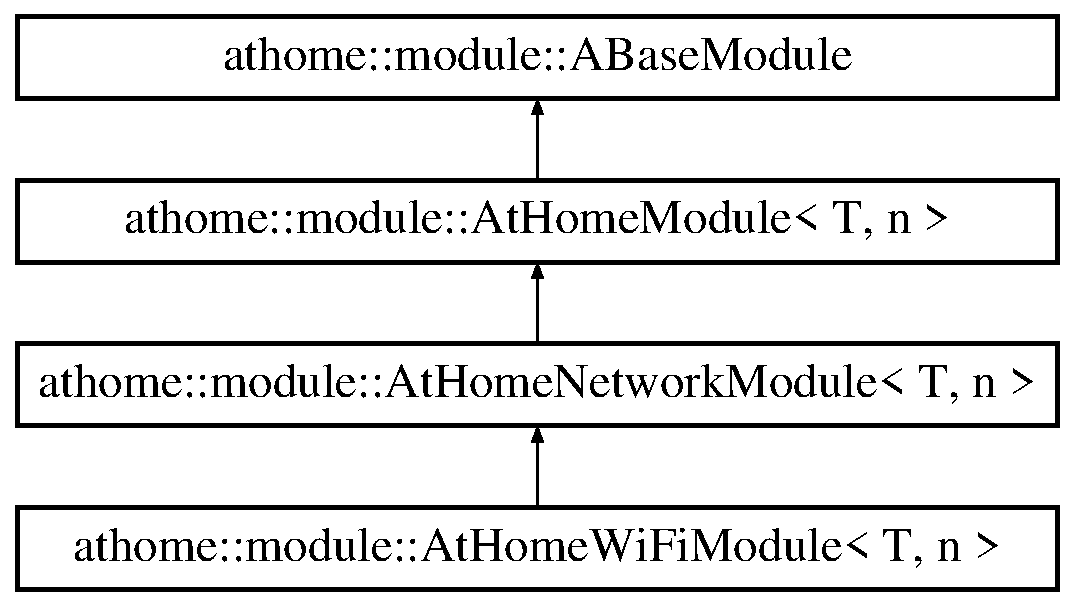
\includegraphics[height=4.000000cm]{classathome_1_1module_1_1_at_home_network_module}
\end{center}
\end{figure}
\subsection*{Public Member Functions}
\begin{DoxyCompactItemize}
\item 
\mbox{\Hypertarget{classathome_1_1module_1_1_at_home_network_module_a1d2da6fec6ca0f45ba75d42a364f8954}\label{classathome_1_1module_1_1_at_home_network_module_a1d2da6fec6ca0f45ba75d42a364f8954}} 
{\bfseries At\+Home\+Network\+Module} (const \mbox{\hyperlink{classathome_1_1module_1_1_at_home_network_module}{At\+Home\+Network\+Module}} \&)=delete
\item 
\mbox{\Hypertarget{classathome_1_1module_1_1_at_home_network_module_abd5f316e792169fd36206b74e47b292d}\label{classathome_1_1module_1_1_at_home_network_module_abd5f316e792169fd36206b74e47b292d}} 
\mbox{\hyperlink{classathome_1_1module_1_1_at_home_network_module}{At\+Home\+Network\+Module}} \& {\bfseries operator=} (const \mbox{\hyperlink{classathome_1_1module_1_1_at_home_network_module}{At\+Home\+Network\+Module}} \&)=delete
\item 
\mbox{\Hypertarget{classathome_1_1module_1_1_at_home_network_module_a274f5a89f9843e67c662f2cf15f6f259}\label{classathome_1_1module_1_1_at_home_network_module_a274f5a89f9843e67c662f2cf15f6f259}} 
virtual void {\bfseries set\+Command\+Plugin} (typename \mbox{\hyperlink{classathome_1_1module_1_1_at_home_module}{At\+Home\+Module}}$<$ T, n $>$\+::At\+Home\+Command\+Plugin plugin)
\item 
\mbox{\Hypertarget{classathome_1_1module_1_1_at_home_network_module_ab63d8d6a336d561e167300bcb455404e}\label{classathome_1_1module_1_1_at_home_network_module_ab63d8d6a336d561e167300bcb455404e}} 
virtual void {\bfseries set\+On\+Backup\+Plugin} (typename \mbox{\hyperlink{classathome_1_1module_1_1_at_home_module}{At\+Home\+Module}}$<$ T, n $>$\+::At\+Home\+Storage\+Plugin plugin)
\item 
\mbox{\Hypertarget{classathome_1_1module_1_1_at_home_network_module_a30d81810788f945d0998ca94d67f3614}\label{classathome_1_1module_1_1_at_home_network_module_a30d81810788f945d0998ca94d67f3614}} 
virtual void {\bfseries set\+On\+Restore\+Plugin} (typename \mbox{\hyperlink{classathome_1_1module_1_1_at_home_module}{At\+Home\+Module}}$<$ T, n $>$\+::At\+Home\+Storage\+Plugin plugin)
\item 
\mbox{\Hypertarget{classathome_1_1module_1_1_at_home_network_module_a34b6119931c22334085816f1060537ee}\label{classathome_1_1module_1_1_at_home_network_module_a34b6119931c22334085816f1060537ee}} 
void {\bfseries set\+Network\+Communicator} (\mbox{\hyperlink{classathome_1_1communication_1_1_a_network_communicator}{communication\+::\+A\+Network\+Communicator}} \&communicator)
\item 
\mbox{\Hypertarget{classathome_1_1module_1_1_at_home_network_module_a52d8845deb42ed1fd8230068f7810ec2}\label{classathome_1_1module_1_1_at_home_network_module_a52d8845deb42ed1fd8230068f7810ec2}} 
void {\bfseries set\+Host} (const \mbox{\hyperlink{structathome_1_1communication_1_1ip_1_1s__host}{communication\+::ip\+::tcp\+\_\+host}} \&host)
\end{DoxyCompactItemize}
\subsection*{Protected Member Functions}
\begin{DoxyCompactItemize}
\item 
\mbox{\Hypertarget{classathome_1_1module_1_1_at_home_network_module_a10787d6a4e5f3007212891f10347dba4}\label{classathome_1_1module_1_1_at_home_network_module_a10787d6a4e5f3007212891f10347dba4}} 
void {\bfseries on\+Network\+Backup} (size\+\_\+t offset, \mbox{\hyperlink{classathome_1_1storage_1_1_i_storage}{storage\+::\+I\+Storage}} \&storage)
\item 
\mbox{\Hypertarget{classathome_1_1module_1_1_at_home_network_module_ae69cb97ae8d892fdf27e5b8ad3dd8072}\label{classathome_1_1module_1_1_at_home_network_module_ae69cb97ae8d892fdf27e5b8ad3dd8072}} 
void {\bfseries on\+Network\+Restore} (size\+\_\+t offset, \mbox{\hyperlink{classathome_1_1storage_1_1_i_storage}{storage\+::\+I\+Storage}} \&storage)
\end{DoxyCompactItemize}
\subsection*{Protected Attributes}
\begin{DoxyCompactItemize}
\item 
\mbox{\Hypertarget{classathome_1_1module_1_1_at_home_network_module_a7c7dba4c623bd8d4d9bb898b6ba9ae63}\label{classathome_1_1module_1_1_at_home_network_module_a7c7dba4c623bd8d4d9bb898b6ba9ae63}} 
\mbox{\hyperlink{classathome_1_1communication_1_1_a_network_communicator}{communication\+::\+A\+Network\+Communicator}} $\ast$ {\bfseries \+\_\+communicator}
\end{DoxyCompactItemize}
\subsection*{Friends}
\begin{DoxyCompactItemize}
\item 
\mbox{\Hypertarget{classathome_1_1module_1_1_at_home_network_module_a5db9640f2e295c39a19645b0d682d7d5}\label{classathome_1_1module_1_1_at_home_network_module_a5db9640f2e295c39a19645b0d682d7d5}} 
class {\bfseries At\+Home\+Module$<$ T, n $>$}
\end{DoxyCompactItemize}
\subsection*{Additional Inherited Members}


The documentation for this class was generated from the following file\+:\begin{DoxyCompactItemize}
\item 
src/At\+Home\+Network\+Module.\+hpp\end{DoxyCompactItemize}

\hypertarget{structathome_1_1module_1_1_at_home_module_1_1_at_home_sensor_measure}{}\section{athome\+:\+:module\+:\+:At\+Home\+Module$<$ T, n $>$\+:\+:At\+Home\+Sensor\+Measure Struct Reference}
\label{structathome_1_1module_1_1_at_home_module_1_1_at_home_sensor_measure}\index{athome\+::module\+::\+At\+Home\+Module$<$ T, n $>$\+::\+At\+Home\+Sensor\+Measure@{athome\+::module\+::\+At\+Home\+Module$<$ T, n $>$\+::\+At\+Home\+Sensor\+Measure}}
\subsection*{Public Attributes}
\begin{DoxyCompactItemize}
\item 
\mbox{\Hypertarget{structathome_1_1module_1_1_at_home_module_1_1_at_home_sensor_measure_a3ea2587077687a8e0951e4f64730b955}\label{structathome_1_1module_1_1_at_home_module_1_1_at_home_sensor_measure_a3ea2587077687a8e0951e4f64730b955}} 
uint8\+\_\+t {\bfseries estimate}
\item 
\mbox{\Hypertarget{structathome_1_1module_1_1_at_home_module_1_1_at_home_sensor_measure_a317f5de5d9032ac12fd0504f709b2e8f}\label{structathome_1_1module_1_1_at_home_module_1_1_at_home_sensor_measure_a317f5de5d9032ac12fd0504f709b2e8f}} 
\mbox{\hyperlink{structathome_1_1utility_1_1units_1_1_unit}{utility\+::units\+::\+Unit}} {\bfseries unit}
\item 
\mbox{\Hypertarget{structathome_1_1module_1_1_at_home_module_1_1_at_home_sensor_measure_ac8060b9a02831d05cf6598558d2314d5}\label{structathome_1_1module_1_1_at_home_module_1_1_at_home_sensor_measure_ac8060b9a02831d05cf6598558d2314d5}} 
\mbox{\hyperlink{classathome_1_1module_1_1_at_home_module_a077afdad789e433d59c588ec6c0f4594}{t\+\_\+timestamp}} {\bfseries timestamp}
\item 
\mbox{\Hypertarget{structathome_1_1module_1_1_at_home_module_1_1_at_home_sensor_measure_a483e0d1c0010854a57e3a1a44f2739c0}\label{structathome_1_1module_1_1_at_home_module_1_1_at_home_sensor_measure_a483e0d1c0010854a57e3a1a44f2739c0}} 
T {\bfseries sample}
\item 
\mbox{\Hypertarget{structathome_1_1module_1_1_at_home_module_1_1_at_home_sensor_measure_a70a00407632c3969cabe019b7e3ba929}\label{structathome_1_1module_1_1_at_home_module_1_1_at_home_sensor_measure_a70a00407632c3969cabe019b7e3ba929}} 
P\+G\+M\+\_\+P {\bfseries label}
\end{DoxyCompactItemize}


The documentation for this struct was generated from the following file\+:\begin{DoxyCompactItemize}
\item 
src/At\+Home\+Module.\+hpp\end{DoxyCompactItemize}

\hypertarget{classathome_1_1module_1_1_at_home_wi_fi_module}{}\section{athome\+:\+:module\+:\+:At\+Home\+Wi\+Fi\+Module$<$ T, n $>$ Class Template Reference}
\label{classathome_1_1module_1_1_at_home_wi_fi_module}\index{athome\+::module\+::\+At\+Home\+Wi\+Fi\+Module$<$ T, n $>$@{athome\+::module\+::\+At\+Home\+Wi\+Fi\+Module$<$ T, n $>$}}


{\ttfamily \#include $<$At\+Home\+Wi\+Fi\+Module.\+hpp$>$}

Inheritance diagram for athome\+:\+:module\+:\+:At\+Home\+Wi\+Fi\+Module$<$ T, n $>$\+:\begin{figure}[H]
\begin{center}
\leavevmode
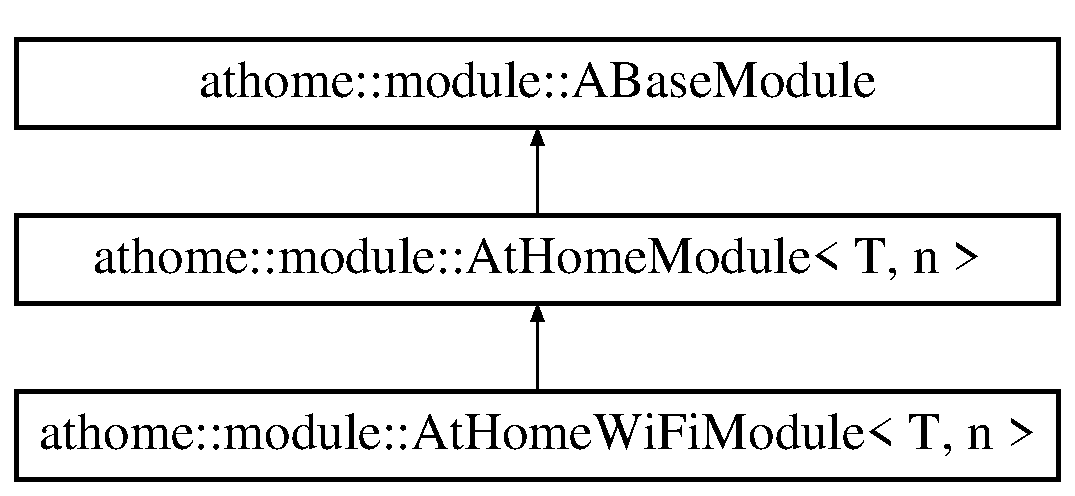
\includegraphics[height=4.000000cm]{classathome_1_1module_1_1_at_home_wi_fi_module}
\end{center}
\end{figure}
\subsection*{Public Member Functions}
\begin{DoxyCompactItemize}
\item 
\mbox{\Hypertarget{classathome_1_1module_1_1_at_home_wi_fi_module_af414ddecde14c57564ccff7ad898b3a0}\label{classathome_1_1module_1_1_at_home_wi_fi_module_af414ddecde14c57564ccff7ad898b3a0}} 
{\bfseries At\+Home\+Wi\+Fi\+Module} (const \mbox{\hyperlink{classathome_1_1module_1_1_at_home_wi_fi_module}{At\+Home\+Wi\+Fi\+Module}} \&)=delete
\item 
\mbox{\Hypertarget{classathome_1_1module_1_1_at_home_wi_fi_module_af3338d83bd96103f7a3a86d5495eb465}\label{classathome_1_1module_1_1_at_home_wi_fi_module_af3338d83bd96103f7a3a86d5495eb465}} 
\mbox{\hyperlink{classathome_1_1module_1_1_at_home_wi_fi_module}{At\+Home\+Wi\+Fi\+Module}} \& {\bfseries operator=} (const \mbox{\hyperlink{classathome_1_1module_1_1_at_home_wi_fi_module}{At\+Home\+Wi\+Fi\+Module}} \&)=delete
\item 
void \mbox{\hyperlink{classathome_1_1module_1_1_at_home_wi_fi_module_a610d2e99c11fdd4b6afbfe65ee2e56d5}{set\+Wi\+Fi\+Communicator}} (\mbox{\hyperlink{classathome_1_1communication_1_1wifi_1_1_a_wi_fi_communicator}{communication\+::wifi\+::\+A\+Wi\+Fi\+Communicator}} \&wifi)
\end{DoxyCompactItemize}
\subsection*{Friends}
\begin{DoxyCompactItemize}
\item 
\mbox{\Hypertarget{classathome_1_1module_1_1_at_home_wi_fi_module_a5db9640f2e295c39a19645b0d682d7d5}\label{classathome_1_1module_1_1_at_home_wi_fi_module_a5db9640f2e295c39a19645b0d682d7d5}} 
class {\bfseries At\+Home\+Module$<$ T, n $>$}
\end{DoxyCompactItemize}
\subsection*{Additional Inherited Members}


\subsection{Detailed Description}
\subsubsection*{template$<$typename T, size\+\_\+t n$>$\newline
class athome\+::module\+::\+At\+Home\+Wi\+Fi\+Module$<$ T, n $>$}

Template class derived from \mbox{\hyperlink{classathome_1_1module_1_1_at_home_module}{athome\+::module\+::\+At\+Home\+Module}}, implementing At\+Home Wi\+Fi extension.

The template parameters are the same than \mbox{\hyperlink{classathome_1_1module_1_1_at_home_module}{athome\+::module\+::\+At\+Home\+Module}} class, taking the type representing in memory a sample from the sensor and the number of samples to buffer.

Example\+:


\begin{DoxyCode}
\textcolor{preprocessor}{#include <AtHome.h>}

AtHomeWiFiModule<uint16\_t, 15> *module = \mbox{\hyperlink{classathome_1_1module_1_1_at_home_module_acc6e7fc0d86f11648fd81729484e546f}{AtHomeModule<uint16\_t, 15>::getInstance}}
      <AtHomeWiFiModule<uint16\_t, 15> >();
ESP8266WiFiCommunicator esp8266(2, 3); \textcolor{comment}{// CH\_ED (enable) pin of the ESP8266 is imagined to be connected to
       pin 2 of the host, and RST (reset) pin is imagined to be connected to pin 3 of the host}

\textcolor{keywordtype}{void} \mbox{\hyperlink{classathome_1_1module_1_1_at_home_module_a5354c736954a788c51e7cf25f6ccf89d}{setup}}() \{
  Serial1.begin(115200);
  esp8266.setStreamToChipset(&Serial1); \textcolor{comment}{// If you're using an Arduino UNO or any other board with only one
       or no UART, use the SoftwareSerial library to create a new Serial instance to pass to this function}
  module->setWiFiCommunicator(esp8266);
\}

\textcolor{keywordtype}{void} loop() \{
  \textcolor{comment}{// Put your code here}
\}
\end{DoxyCode}
 

\subsection{Member Function Documentation}
\mbox{\Hypertarget{classathome_1_1module_1_1_at_home_wi_fi_module_a610d2e99c11fdd4b6afbfe65ee2e56d5}\label{classathome_1_1module_1_1_at_home_wi_fi_module_a610d2e99c11fdd4b6afbfe65ee2e56d5}} 
\index{athome\+::module\+::\+At\+Home\+Wi\+Fi\+Module@{athome\+::module\+::\+At\+Home\+Wi\+Fi\+Module}!set\+Wi\+Fi\+Communicator@{set\+Wi\+Fi\+Communicator}}
\index{set\+Wi\+Fi\+Communicator@{set\+Wi\+Fi\+Communicator}!athome\+::module\+::\+At\+Home\+Wi\+Fi\+Module@{athome\+::module\+::\+At\+Home\+Wi\+Fi\+Module}}
\subsubsection{\texorpdfstring{set\+Wi\+Fi\+Communicator()}{setWiFiCommunicator()}}
{\footnotesize\ttfamily template$<$typename T , size\+\_\+t n$>$ \\
void \mbox{\hyperlink{classathome_1_1module_1_1_at_home_wi_fi_module}{athome\+::module\+::\+At\+Home\+Wi\+Fi\+Module}}$<$ T, n $>$\+::set\+Wi\+Fi\+Communicator (\begin{DoxyParamCaption}\item[{\mbox{\hyperlink{classathome_1_1communication_1_1wifi_1_1_a_wi_fi_communicator}{communication\+::wifi\+::\+A\+Wi\+Fi\+Communicator}} \&}]{wifi }\end{DoxyParamCaption})\hspace{0.3cm}{\ttfamily [inline]}}

Set the Wi\+Fi object used for wireless communication by passing it as reference.

See class example for usage of this method. 

The documentation for this class was generated from the following file\+:\begin{DoxyCompactItemize}
\item 
src/At\+Home\+Wi\+Fi\+Module.\+hpp\end{DoxyCompactItemize}

\hypertarget{classathome_1_1power_1_1_a_v_r_power_management}{}\section{athome\+:\+:power\+:\+:A\+V\+R\+Power\+Management Class Reference}
\label{classathome_1_1power_1_1_a_v_r_power_management}\index{athome\+::power\+::\+A\+V\+R\+Power\+Management@{athome\+::power\+::\+A\+V\+R\+Power\+Management}}
Inheritance diagram for athome\+:\+:power\+:\+:A\+V\+R\+Power\+Management\+:\begin{figure}[H]
\begin{center}
\leavevmode
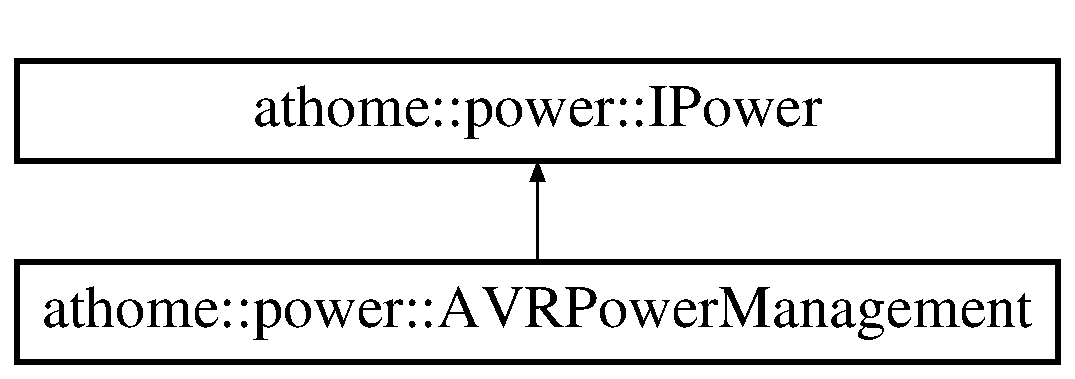
\includegraphics[height=2.000000cm]{classathome_1_1power_1_1_a_v_r_power_management}
\end{center}
\end{figure}
\subsection*{Public Member Functions}
\begin{DoxyCompactItemize}
\item 
\mbox{\Hypertarget{classathome_1_1power_1_1_a_v_r_power_management_ae272a5c17f8cad814f7da51324f96757}\label{classathome_1_1power_1_1_a_v_r_power_management_ae272a5c17f8cad814f7da51324f96757}} 
{\bfseries A\+V\+R\+Power\+Management} (const \mbox{\hyperlink{classathome_1_1power_1_1_a_v_r_power_management}{A\+V\+R\+Power\+Management}} \&)
\item 
\mbox{\Hypertarget{classathome_1_1power_1_1_a_v_r_power_management_aca40015de3d71ec77b2ef4ad458a0db1}\label{classathome_1_1power_1_1_a_v_r_power_management_aca40015de3d71ec77b2ef4ad458a0db1}} 
\mbox{\hyperlink{classathome_1_1power_1_1_a_v_r_power_management}{A\+V\+R\+Power\+Management}} \& {\bfseries operator=} (const \mbox{\hyperlink{classathome_1_1power_1_1_a_v_r_power_management}{A\+V\+R\+Power\+Management}} \&)
\item 
\mbox{\Hypertarget{classathome_1_1power_1_1_a_v_r_power_management_a8d335811814a50460c9b6d705eab46e2}\label{classathome_1_1power_1_1_a_v_r_power_management_a8d335811814a50460c9b6d705eab46e2}} 
const \mbox{\hyperlink{structathome_1_1power_1_1_i_power_1_1_power_info}{Power\+Info}} $\ast$ {\bfseries get\+Power\+Info} ()
\item 
\mbox{\Hypertarget{classathome_1_1power_1_1_a_v_r_power_management_a14aef66965c95b5855a7375e80d93721}\label{classathome_1_1power_1_1_a_v_r_power_management_a14aef66965c95b5855a7375e80d93721}} 
void {\bfseries sleep} (S\+L\+E\+E\+P\+\_\+\+M\+O\+DE, uint32\+\_\+t)
\end{DoxyCompactItemize}
\subsection*{Protected Member Functions}
\begin{DoxyCompactItemize}
\item 
\mbox{\Hypertarget{classathome_1_1power_1_1_a_v_r_power_management_ac5410cf1848b98b505afbd6296218ded}\label{classathome_1_1power_1_1_a_v_r_power_management_ac5410cf1848b98b505afbd6296218ded}} 
void {\bfseries \+\_\+setup\+Watchdog} ()
\end{DoxyCompactItemize}
\subsection*{Additional Inherited Members}


The documentation for this class was generated from the following files\+:\begin{DoxyCompactItemize}
\item 
src/A\+V\+R\+Power\+Manager.\+hpp\item 
src/power/A\+V\+R\+Power\+Manager.\+cpp\end{DoxyCompactItemize}

\hypertarget{classathome_1_1communication_1_1wifi_1_1_a_wi_fi_communicator}{}\section{athome\+:\+:communication\+:\+:wifi\+:\+:A\+Wi\+Fi\+Communicator Class Reference}
\label{classathome_1_1communication_1_1wifi_1_1_a_wi_fi_communicator}\index{athome\+::communication\+::wifi\+::\+A\+Wi\+Fi\+Communicator@{athome\+::communication\+::wifi\+::\+A\+Wi\+Fi\+Communicator}}


{\ttfamily \#include $<$A\+Wi\+Fi\+Communicator.\+hpp$>$}

Inheritance diagram for athome\+:\+:communication\+:\+:wifi\+:\+:A\+Wi\+Fi\+Communicator\+:\begin{figure}[H]
\begin{center}
\leavevmode
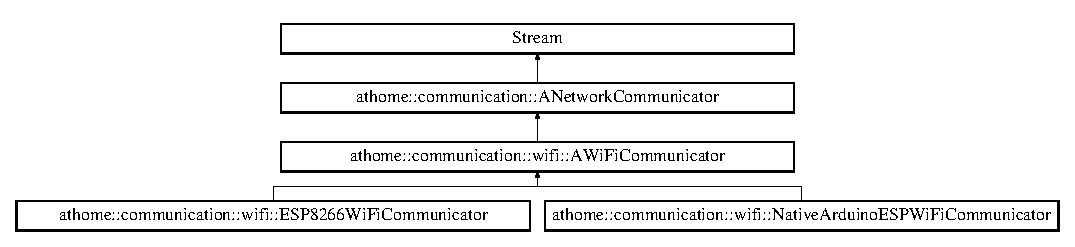
\includegraphics[height=2.871795cm]{classathome_1_1communication_1_1wifi_1_1_a_wi_fi_communicator}
\end{center}
\end{figure}
\subsection*{Public Member Functions}
\begin{DoxyCompactItemize}
\item 
\mbox{\hyperlink{classathome_1_1communication_1_1wifi_1_1_a_wi_fi_communicator_a0098148fe8d0eeee99b7f8f72a72a900}{A\+Wi\+Fi\+Communicator}} (const \mbox{\hyperlink{structathome_1_1communication_1_1wifi_1_1s__wifi__access__point}{Wi\+Fi\+\_\+ap}} $\ast$=nullptr, const \mbox{\hyperlink{structathome_1_1communication_1_1wifi_1_1s__wifi__client}{Wi\+Fi\+\_\+client}} $\ast$=nullptr, const wifi\+\_\+mode=S\+T\+A\+T\+I\+ON, Stream $\ast$=nullptr)
\item 
\mbox{\Hypertarget{classathome_1_1communication_1_1wifi_1_1_a_wi_fi_communicator_a5d9a73879f80042bf3c0da09ff32f0b5}\label{classathome_1_1communication_1_1wifi_1_1_a_wi_fi_communicator_a5d9a73879f80042bf3c0da09ff32f0b5}} 
{\bfseries A\+Wi\+Fi\+Communicator} (const \mbox{\hyperlink{classathome_1_1communication_1_1wifi_1_1_a_wi_fi_communicator}{A\+Wi\+Fi\+Communicator}} \&)=delete
\item 
\mbox{\Hypertarget{classathome_1_1communication_1_1wifi_1_1_a_wi_fi_communicator_afc2748d9230575335d3cfd7936ff26ee}\label{classathome_1_1communication_1_1wifi_1_1_a_wi_fi_communicator_afc2748d9230575335d3cfd7936ff26ee}} 
\mbox{\hyperlink{classathome_1_1communication_1_1wifi_1_1_a_wi_fi_communicator}{A\+Wi\+Fi\+Communicator}} \& {\bfseries operator=} (const \mbox{\hyperlink{classathome_1_1communication_1_1wifi_1_1_a_wi_fi_communicator}{A\+Wi\+Fi\+Communicator}} \&)=delete
\item 
virtual int \mbox{\hyperlink{classathome_1_1communication_1_1wifi_1_1_a_wi_fi_communicator_a309927109fbc19aa0fb2afb71d50bbf9}{connect}} ()=0
\item 
virtual int \mbox{\hyperlink{classathome_1_1communication_1_1wifi_1_1_a_wi_fi_communicator_a6131240ac0daa0f9fb4d46871feea4c2}{disconnect}} ()=0
\item 
virtual bool \mbox{\hyperlink{classathome_1_1communication_1_1wifi_1_1_a_wi_fi_communicator_a578087d01c814481d89ea702a6d7ed01}{is\+Connected}} () const =0
\item 
const \mbox{\hyperlink{structathome_1_1communication_1_1wifi_1_1s__wifi__access__point}{Wi\+Fi\+\_\+ap}} \& \mbox{\hyperlink{classathome_1_1communication_1_1wifi_1_1_a_wi_fi_communicator_abef86486512e4a39d61df3b27effcc87}{get\+Access\+Point}} () const
\item 
const \mbox{\hyperlink{structathome_1_1communication_1_1wifi_1_1s__wifi__client}{Wi\+Fi\+\_\+client}} \& \mbox{\hyperlink{classathome_1_1communication_1_1wifi_1_1_a_wi_fi_communicator_afcc41f462a12c8348148c915dcafd1a0}{get\+Connection\+Addresses}} () const
\item 
wifi\+\_\+mode \mbox{\hyperlink{classathome_1_1communication_1_1wifi_1_1_a_wi_fi_communicator_adebc335ea6408a90919f396f06260b13}{get\+Wi\+Fi\+Mode}} () const
\item 
void \mbox{\hyperlink{classathome_1_1communication_1_1wifi_1_1_a_wi_fi_communicator_a2b802d934022436e029fc31b3e84d321}{set\+Access\+Point}} (const \mbox{\hyperlink{structathome_1_1communication_1_1wifi_1_1s__wifi__access__point}{Wi\+Fi\+\_\+ap}} \&)
\item 
void \mbox{\hyperlink{classathome_1_1communication_1_1wifi_1_1_a_wi_fi_communicator_a31fb91672f298718d99bb9776dfe46c9}{set\+Connection\+Addresses}} (const \mbox{\hyperlink{structathome_1_1communication_1_1wifi_1_1s__wifi__client}{Wi\+Fi\+\_\+client}} \&)
\item 
void \mbox{\hyperlink{classathome_1_1communication_1_1wifi_1_1_a_wi_fi_communicator_a28538cf510da8b59056b2533a6e53bcc}{set\+Wi\+Fi\+Mode}} (wifi\+\_\+mode)
\item 
void \mbox{\hyperlink{classathome_1_1communication_1_1wifi_1_1_a_wi_fi_communicator_a42f2ad88713db57bd9e9670f090924de}{set\+Stream\+To\+Chipset}} (Stream $\ast$)
\item 
\mbox{\Hypertarget{classathome_1_1communication_1_1wifi_1_1_a_wi_fi_communicator_a9743bf55f6145e641e3cf35a072c14e1}\label{classathome_1_1communication_1_1wifi_1_1_a_wi_fi_communicator_a9743bf55f6145e641e3cf35a072c14e1}} 
bool {\bfseries is\+Access\+Point\+Configured} ()
\end{DoxyCompactItemize}
\subsection*{Protected Attributes}
\begin{DoxyCompactItemize}
\item 
\mbox{\Hypertarget{classathome_1_1communication_1_1wifi_1_1_a_wi_fi_communicator_a857f4193bdf63fcfdddeaf43f945ed50}\label{classathome_1_1communication_1_1wifi_1_1_a_wi_fi_communicator_a857f4193bdf63fcfdddeaf43f945ed50}} 
wifi\+\_\+mode {\bfseries \+\_\+mode}
\item 
\mbox{\Hypertarget{classathome_1_1communication_1_1wifi_1_1_a_wi_fi_communicator_a07a54c2f10295708f14d6a9069612f48}\label{classathome_1_1communication_1_1wifi_1_1_a_wi_fi_communicator_a07a54c2f10295708f14d6a9069612f48}} 
Stream $\ast$ {\bfseries \+\_\+stream}
\item 
\mbox{\Hypertarget{classathome_1_1communication_1_1wifi_1_1_a_wi_fi_communicator_a4d1d5dae7e80603205321585a8861bb8}\label{classathome_1_1communication_1_1wifi_1_1_a_wi_fi_communicator_a4d1d5dae7e80603205321585a8861bb8}} 
\mbox{\hyperlink{structathome_1_1communication_1_1wifi_1_1s__wifi__access__point}{Wi\+Fi\+\_\+ap}} {\bfseries \+\_\+ap}
\item 
\mbox{\Hypertarget{classathome_1_1communication_1_1wifi_1_1_a_wi_fi_communicator_af249e6e9eff32fed22de39a5b7c62b49}\label{classathome_1_1communication_1_1wifi_1_1_a_wi_fi_communicator_af249e6e9eff32fed22de39a5b7c62b49}} 
\mbox{\hyperlink{structathome_1_1communication_1_1wifi_1_1s__wifi__client}{Wi\+Fi\+\_\+client}} {\bfseries \+\_\+me}
\end{DoxyCompactItemize}


\subsection{Detailed Description}
Abstract class derived from Stream, declaring some new Wi\+Fi common interface methods, and implementing some utility methods for these {\ttfamily Stream}s

Here\textquotesingle{}s a simple example of implementing a U\+A\+RT to Wi\+Fi chipset pre-\/configured to connect a Wi\+Fi network and transparently bridge the serial connection always connected to Serial Stream\+:


\begin{DoxyCode}
\textcolor{preprocessor}{#include <AWiFiCommunicator.hpp>}

\textcolor{keyword}{using} \mbox{\hyperlink{classathome_1_1communication_1_1wifi_1_1_a_wi_fi_communicator}{athome::communication::wifi::AWiFiCommunicator}};

\textcolor{keyword}{class }MyUARTBridge : \textcolor{keyword}{public} \mbox{\hyperlink{classathome_1_1communication_1_1wifi_1_1_a_wi_fi_communicator_a0098148fe8d0eeee99b7f8f72a72a900}{AWiFiCommunicator}} \{
  \textcolor{keyword}{public}:
    MyUARTBridge():\mbox{\hyperlink{classathome_1_1communication_1_1wifi_1_1_a_wi_fi_communicator_a0098148fe8d0eeee99b7f8f72a72a900}{AWiFiCommunicator}}() \{
      \_stream = &Serial;
    \}
    ~MyUARTBridge() \{\}

    \textcolor{keywordtype}{int} \mbox{\hyperlink{classathome_1_1communication_1_1_a_network_communicator_a2bf367d03c98e8523fda71dd43ffa2fb}{available}}() \{ \textcolor{keywordflow}{return} \_stream->available(); \}
    \textcolor{keywordtype}{int} \mbox{\hyperlink{classathome_1_1communication_1_1_a_network_communicator_a88d3c4366daf48865ab48b22eb62d610}{read}}() \{ \textcolor{keywordflow}{return} \_stream->return(); \}
    \textcolor{keywordtype}{int} \mbox{\hyperlink{classathome_1_1communication_1_1_a_network_communicator_ad06ecdc94aa77b1bab934b85bed2ac7d}{peek}}() \{ \textcolor{keywordflow}{return} \_stream->peek(); \}
    \textcolor{keywordtype}{size\_t} \mbox{\hyperlink{classathome_1_1communication_1_1_a_network_communicator_a87adf68359a4ec5b0a38bea529ebf732}{write}}(uint8\_t data) \{ \textcolor{keywordflow}{return} \_stream->write(data); \}
    \textcolor{keywordtype}{int} \mbox{\hyperlink{classathome_1_1communication_1_1wifi_1_1_a_wi_fi_communicator_a309927109fbc19aa0fb2afb71d50bbf9}{connect}}() \{ \textcolor{keywordflow}{return} 0; \}
    \textcolor{keywordtype}{int} \mbox{\hyperlink{classathome_1_1communication_1_1wifi_1_1_a_wi_fi_communicator_a6131240ac0daa0f9fb4d46871feea4c2}{disconnect}}() \{ \textcolor{keywordflow}{return} 0; \}
    \textcolor{keywordtype}{int} \mbox{\hyperlink{classathome_1_1communication_1_1_a_network_communicator_a370176dae8f38225446e83a132dbcff7}{connectToHost}}() \{ \textcolor{keywordflow}{return} 0; \}
    \textcolor{keywordtype}{int} \mbox{\hyperlink{classathome_1_1communication_1_1_a_network_communicator_a025b7fbe9b3c4452fcf1925d766324eb}{disconnectFromHost}}() \{ \textcolor{keywordflow}{return} 0; \}
    \textcolor{keywordtype}{bool} \mbox{\hyperlink{classathome_1_1communication_1_1wifi_1_1_a_wi_fi_communicator_a578087d01c814481d89ea702a6d7ed01}{isConnected}}() \{ \textcolor{keywordflow}{return} \textcolor{keyword}{true}; \}
\}
\end{DoxyCode}
 

\subsection{Constructor \& Destructor Documentation}
\mbox{\Hypertarget{classathome_1_1communication_1_1wifi_1_1_a_wi_fi_communicator_a0098148fe8d0eeee99b7f8f72a72a900}\label{classathome_1_1communication_1_1wifi_1_1_a_wi_fi_communicator_a0098148fe8d0eeee99b7f8f72a72a900}} 
\index{athome\+::communication\+::wifi\+::\+A\+Wi\+Fi\+Communicator@{athome\+::communication\+::wifi\+::\+A\+Wi\+Fi\+Communicator}!A\+Wi\+Fi\+Communicator@{A\+Wi\+Fi\+Communicator}}
\index{A\+Wi\+Fi\+Communicator@{A\+Wi\+Fi\+Communicator}!athome\+::communication\+::wifi\+::\+A\+Wi\+Fi\+Communicator@{athome\+::communication\+::wifi\+::\+A\+Wi\+Fi\+Communicator}}
\subsubsection{\texorpdfstring{A\+Wi\+Fi\+Communicator()}{AWiFiCommunicator()}}
{\footnotesize\ttfamily athome\+::communication\+::wifi\+::\+A\+Wi\+Fi\+Communicator\+::\+A\+Wi\+Fi\+Communicator (\begin{DoxyParamCaption}\item[{const \mbox{\hyperlink{structathome_1_1communication_1_1wifi_1_1s__wifi__access__point}{Wi\+Fi\+\_\+ap}} $\ast$}]{ap = {\ttfamily nullptr},  }\item[{const \mbox{\hyperlink{structathome_1_1communication_1_1wifi_1_1s__wifi__client}{Wi\+Fi\+\_\+client}} $\ast$}]{client = {\ttfamily nullptr},  }\item[{const wifi\+\_\+mode}]{mode = {\ttfamily STATION},  }\item[{Stream $\ast$}]{stream = {\ttfamily nullptr} }\end{DoxyParamCaption})}

Base constructor taking optional parameters to initialize instance attributes. 

\subsection{Member Function Documentation}
\mbox{\Hypertarget{classathome_1_1communication_1_1wifi_1_1_a_wi_fi_communicator_a309927109fbc19aa0fb2afb71d50bbf9}\label{classathome_1_1communication_1_1wifi_1_1_a_wi_fi_communicator_a309927109fbc19aa0fb2afb71d50bbf9}} 
\index{athome\+::communication\+::wifi\+::\+A\+Wi\+Fi\+Communicator@{athome\+::communication\+::wifi\+::\+A\+Wi\+Fi\+Communicator}!connect@{connect}}
\index{connect@{connect}!athome\+::communication\+::wifi\+::\+A\+Wi\+Fi\+Communicator@{athome\+::communication\+::wifi\+::\+A\+Wi\+Fi\+Communicator}}
\subsubsection{\texorpdfstring{connect()}{connect()}}
{\footnotesize\ttfamily virtual int athome\+::communication\+::wifi\+::\+A\+Wi\+Fi\+Communicator\+::connect (\begin{DoxyParamCaption}{ }\end{DoxyParamCaption})\hspace{0.3cm}{\ttfamily [pure virtual]}}

Virtual method used to implement connection to Wi\+Fi network through the adapter.

A return value of 0 is expected to indicate the connection was successful, otherwise all other values are available for error codes.

Example\+:


\begin{DoxyCode}
\textcolor{preprocessor}{#include <string.h>}
\textcolor{preprocessor}{#include <AtHome.h>}

\textcolor{keyword}{using} \mbox{\hyperlink{structathome_1_1communication_1_1wifi_1_1s__wifi__access__point}{athome::communication::wifi::WiFi\_ap}}; \textcolor{comment}{// Use this to not have to}
\mbox{\hyperlink{classathome_1_1communication_1_1_a_network_communicator_a87adf68359a4ec5b0a38bea529ebf732}{write}} the full \textcolor{keyword}{namespace }names further using
\mbox{\hyperlink{namespaceathome}{athome}}::communication::wifi::AWiFiCommunicator;

void my\_function\_connecting\_wifi\_to\_network\_called\_foobar(AWiFiCommunicator
&wifi) \{ WiFi\_ap network; \textcolor{comment}{// Declare a WiFi\_ap structure}
  strncpy(network.ssid, \textcolor{stringliteral}{"foobar"}, \textcolor{keyword}{sizeof}(network.ssid)); \textcolor{comment}{// Copy "foobar"}
in the ssid field of the structure, as the SSID of a WiFi network is the
name shown to humans strncpy(network.password, \textcolor{stringliteral}{"12345678"},
\textcolor{keyword}{sizeof}(network.password)); \textcolor{comment}{// Copy "12345678" in the password field, to set}
the password used by the WiFi network wifi.setAccessPoint(network); \textcolor{comment}{// Set}
the WiFi network parameters we created \textcolor{keywordflow}{if} (!wifi.connect()) \{ \textcolor{comment}{// Connect to}
\textcolor{keyword}{this} network Serial.println(\textcolor{stringliteral}{"Successfully connected to WiFi network"}); \}
\textcolor{keywordflow}{else} \{ Serial.println(\textcolor{stringliteral}{"Connection to WiFi network failed"});
  \}
\}
\end{DoxyCode}
 

Implemented in \mbox{\hyperlink{classathome_1_1communication_1_1wifi_1_1_native_arduino_e_s_p_wi_fi_communicator_abc07f2d953fa91f86b8919858e10bbd7}{athome\+::communication\+::wifi\+::\+Native\+Arduino\+E\+S\+P\+Wi\+Fi\+Communicator}}, and \mbox{\hyperlink{classathome_1_1communication_1_1wifi_1_1_e_s_p8266_wi_fi_communicator_a58cc439be2f368b346bbbe1601a9b675}{athome\+::communication\+::wifi\+::\+E\+S\+P8266\+Wi\+Fi\+Communicator}}.

\mbox{\Hypertarget{classathome_1_1communication_1_1wifi_1_1_a_wi_fi_communicator_a6131240ac0daa0f9fb4d46871feea4c2}\label{classathome_1_1communication_1_1wifi_1_1_a_wi_fi_communicator_a6131240ac0daa0f9fb4d46871feea4c2}} 
\index{athome\+::communication\+::wifi\+::\+A\+Wi\+Fi\+Communicator@{athome\+::communication\+::wifi\+::\+A\+Wi\+Fi\+Communicator}!disconnect@{disconnect}}
\index{disconnect@{disconnect}!athome\+::communication\+::wifi\+::\+A\+Wi\+Fi\+Communicator@{athome\+::communication\+::wifi\+::\+A\+Wi\+Fi\+Communicator}}
\subsubsection{\texorpdfstring{disconnect()}{disconnect()}}
{\footnotesize\ttfamily virtual int athome\+::communication\+::wifi\+::\+A\+Wi\+Fi\+Communicator\+::disconnect (\begin{DoxyParamCaption}{ }\end{DoxyParamCaption})\hspace{0.3cm}{\ttfamily [pure virtual]}}

Virtual method used to implement disconnection of the current Wi\+Fi network through the adapter.

A return value of 0 is expected to indicate success, otherwise all other values are available for error codes.

Usage is as simple as this\+:


\begin{DoxyCode}
\textcolor{preprocessor}{#include <AWiFiCommunicator.hpp>}

\textcolor{keyword}{using} \mbox{\hyperlink{classathome_1_1communication_1_1wifi_1_1_a_wi_fi_communicator}{athome::communication::wifi::AWiFiCommunicator}};

\textcolor{keywordtype}{void} my\_function\_disconnecting\_wifi\_adapters(AWiFiCommuncator &wifi) \{
  \textcolor{keywordflow}{if} (!wifi.disconnect()) \{
    Serial.println(\textcolor{stringliteral}{"Successfully disconnected from WiFi network"});
  \} \textcolor{keywordflow}{else} \{
    Serial.println(\textcolor{stringliteral}{"Failed to disconnect from WiFi network"}); \textcolor{comment}{// Is that}
really possible? In \textcolor{keywordflow}{case} we\textcolor{stringliteral}{'re stuck, it'}s a problem where the \textcolor{stringliteral}{"have you}
\textcolor{stringliteral}{tried turning it off and on again?"} rocks ;)
\}
\end{DoxyCode}
 

Implemented in \mbox{\hyperlink{classathome_1_1communication_1_1wifi_1_1_native_arduino_e_s_p_wi_fi_communicator_a3787e850d48d149ee1392ebfb2920bb3}{athome\+::communication\+::wifi\+::\+Native\+Arduino\+E\+S\+P\+Wi\+Fi\+Communicator}}, and \mbox{\hyperlink{classathome_1_1communication_1_1wifi_1_1_e_s_p8266_wi_fi_communicator_a7e53e10b858aebc5e7c6c0ea6007f84a}{athome\+::communication\+::wifi\+::\+E\+S\+P8266\+Wi\+Fi\+Communicator}}.

\mbox{\Hypertarget{classathome_1_1communication_1_1wifi_1_1_a_wi_fi_communicator_abef86486512e4a39d61df3b27effcc87}\label{classathome_1_1communication_1_1wifi_1_1_a_wi_fi_communicator_abef86486512e4a39d61df3b27effcc87}} 
\index{athome\+::communication\+::wifi\+::\+A\+Wi\+Fi\+Communicator@{athome\+::communication\+::wifi\+::\+A\+Wi\+Fi\+Communicator}!get\+Access\+Point@{get\+Access\+Point}}
\index{get\+Access\+Point@{get\+Access\+Point}!athome\+::communication\+::wifi\+::\+A\+Wi\+Fi\+Communicator@{athome\+::communication\+::wifi\+::\+A\+Wi\+Fi\+Communicator}}
\subsubsection{\texorpdfstring{get\+Access\+Point()}{getAccessPoint()}}
{\footnotesize\ttfamily const \mbox{\hyperlink{structathome_1_1communication_1_1wifi_1_1s__wifi__access__point}{Wi\+Fi\+\_\+ap}} \& athome\+::communication\+::wifi\+::\+A\+Wi\+Fi\+Communicator\+::get\+Access\+Point (\begin{DoxyParamCaption}{ }\end{DoxyParamCaption}) const}

Method returning a reference on the current configured access point into the instance of \mbox{\hyperlink{classathome_1_1communication_1_1wifi_1_1_a_wi_fi_communicator}{A\+Wi\+Fi\+Communicator}}.

See athome\+::communication\+::wifi\+::\+Wi\+Fi\+\_\+ap for more information on the content of this structure.

Example\+:


\begin{DoxyCode}
\textcolor{preprocessor}{#include <AtHome.h>}

\textcolor{keyword}{using} \mbox{\hyperlink{structathome_1_1communication_1_1wifi_1_1s__wifi__access__point}{athome::communication::wifi::WiFi\_ap}};
\textcolor{keyword}{using} \mbox{\hyperlink{classathome_1_1communication_1_1wifi_1_1_a_wi_fi_communicator}{athome::communication::wifi::AWiFiCommunicator}};

\textcolor{keywordtype}{void} my\_function\_printing\_current\_access\_point\_info(\textcolor{keyword}{const} \mbox{\hyperlink{classathome_1_1communication_1_1wifi_1_1_a_wi_fi_communicator_a0098148fe8d0eeee99b7f8f72a72a900}{AWiFiCommunicator}}
&wifi) \{ \textcolor{keyword}{const} WiFi\_ap &access\_point = wifi.getAccessPoint;
  Serial.print(\textcolor{stringliteral}{"Network name: "});
  Serial.println(access\_point.ssid);
  Serial.print(\textcolor{stringliteral}{"Password: "});
  Serial.println(access\_point.password);
\}
\end{DoxyCode}
 \mbox{\Hypertarget{classathome_1_1communication_1_1wifi_1_1_a_wi_fi_communicator_afcc41f462a12c8348148c915dcafd1a0}\label{classathome_1_1communication_1_1wifi_1_1_a_wi_fi_communicator_afcc41f462a12c8348148c915dcafd1a0}} 
\index{athome\+::communication\+::wifi\+::\+A\+Wi\+Fi\+Communicator@{athome\+::communication\+::wifi\+::\+A\+Wi\+Fi\+Communicator}!get\+Connection\+Addresses@{get\+Connection\+Addresses}}
\index{get\+Connection\+Addresses@{get\+Connection\+Addresses}!athome\+::communication\+::wifi\+::\+A\+Wi\+Fi\+Communicator@{athome\+::communication\+::wifi\+::\+A\+Wi\+Fi\+Communicator}}
\subsubsection{\texorpdfstring{get\+Connection\+Addresses()}{getConnectionAddresses()}}
{\footnotesize\ttfamily const \mbox{\hyperlink{structathome_1_1communication_1_1wifi_1_1s__wifi__client}{Wi\+Fi\+\_\+client}} \& athome\+::communication\+::wifi\+::\+A\+Wi\+Fi\+Communicator\+::get\+Connection\+Addresses (\begin{DoxyParamCaption}{ }\end{DoxyParamCaption}) const}

Method returning a reference on the current (or last if the module is currently disconnected) IP and M\+AC addresses of this instance of \mbox{\hyperlink{classathome_1_1communication_1_1wifi_1_1_a_wi_fi_communicator}{A\+Wi\+Fi\+Communicator}}.

See athome\+::communication\+::wifi\+::\+Wi\+Fi\+\_\+client for more information on the content of this structure.

Example\+:


\begin{DoxyCode}
\textcolor{preprocessor}{#include <stdio.h>}
\textcolor{preprocessor}{#include <AtHome.h>}

\textcolor{keyword}{using} \mbox{\hyperlink{structathome_1_1communication_1_1wifi_1_1s__wifi__client}{athome::communication::wifi::WiFi\_client}};
\textcolor{keyword}{using} \mbox{\hyperlink{classathome_1_1communication_1_1wifi_1_1_a_wi_fi_communicator}{athome::communication::wifi::AWiFiCommunicator}};

\textcolor{keywordtype}{void} my\_function\_printing\_current\_ip\_and\_mac\_addresses(\textcolor{keyword}{const}
\mbox{\hyperlink{classathome_1_1communication_1_1wifi_1_1_a_wi_fi_communicator_a0098148fe8d0eeee99b7f8f72a72a900}{AWiFiCommunicator}} &wifi) \{ \textcolor{keyword}{const} WiFi\_client &addresses =
wifi.getConnectionAddresses(); \textcolor{keywordtype}{char} my\_ipv4[16]; \textcolor{keywordtype}{char} my\_mac[18];
  snprintf(my\_ipv4, 16, \textcolor{stringliteral}{"%hhu.%hhu.%hhu.%hhu"}, addresses.ipv4[0],
addresses.ipv4[1], addresses.ipv4[2], addresses.ipv4[3]);
  \textcolor{comment}{// Note: For MAC address conversion, if you're compiler is broken and}
doesn\textcolor{stringliteral}{'t promote char'}s to int, see \textcolor{keyword}{this} StackOverflow \textcolor{keywordflow}{for} fix:
  \textcolor{comment}{//}
https:\textcolor{comment}{//stackoverflow.com/questions/12344814/how-to-print-unsigned-char-as-2-digit-hex-value-in-c}
  snprintf(my\_mac, 18, \textcolor{stringliteral}{"%02x-%02x-%02x-%02x-%02x-%02x"},
           addresses.mac[0], addresses.mac[1], addresses.mac[2],
addresses.mac[3], addresses.mac[4], addresses.mac[5]); Serial.print(\textcolor{stringliteral}{"IPv4:}
\textcolor{stringliteral}{"}); Serial.println(my\_ipv4); Serial.print(\textcolor{stringliteral}{"MAC: "}); Serial.println(my\_mac);
\}
\end{DoxyCode}
 \mbox{\Hypertarget{classathome_1_1communication_1_1wifi_1_1_a_wi_fi_communicator_adebc335ea6408a90919f396f06260b13}\label{classathome_1_1communication_1_1wifi_1_1_a_wi_fi_communicator_adebc335ea6408a90919f396f06260b13}} 
\index{athome\+::communication\+::wifi\+::\+A\+Wi\+Fi\+Communicator@{athome\+::communication\+::wifi\+::\+A\+Wi\+Fi\+Communicator}!get\+Wi\+Fi\+Mode@{get\+Wi\+Fi\+Mode}}
\index{get\+Wi\+Fi\+Mode@{get\+Wi\+Fi\+Mode}!athome\+::communication\+::wifi\+::\+A\+Wi\+Fi\+Communicator@{athome\+::communication\+::wifi\+::\+A\+Wi\+Fi\+Communicator}}
\subsubsection{\texorpdfstring{get\+Wi\+Fi\+Mode()}{getWiFiMode()}}
{\footnotesize\ttfamily wifi\+\_\+mode athome\+::communication\+::wifi\+::\+A\+Wi\+Fi\+Communicator\+::get\+Wi\+Fi\+Mode (\begin{DoxyParamCaption}{ }\end{DoxyParamCaption}) const}

Method returning a value of athome\+::communication\+::ip\+::wifi\+\_\+mode enumeration, being S\+T\+A\+T\+I\+ON if the adapter connects to a Wi\+Fi network, or A\+C\+C\+E\+S\+S\+\_\+\+P\+O\+I\+NT if it creates one.

See athome\+::communication\+::ip\+::wifi\+\_\+mode for more information about this enumeration.

Example\+:


\begin{DoxyCode}
\textcolor{preprocessor}{#include <AtHome.h>}

\textcolor{keyword}{using} athome::communication::wifi::wifi\_mode;
\textcolor{keyword}{using} \mbox{\hyperlink{classathome_1_1communication_1_1wifi_1_1_a_wi_fi_communicator}{athome::communication::wifi::AWiFiCommunicator}};

\textcolor{keywordtype}{void} my\_function\_printing\_current\_wifi\_mode(\textcolor{keyword}{const} \mbox{\hyperlink{classathome_1_1communication_1_1wifi_1_1_a_wi_fi_communicator_a0098148fe8d0eeee99b7f8f72a72a900}{AWiFiCommunicator}} &wifi)
\{ wifi\_mode mode = wifi.getWiFiMode(); \textcolor{keywordflow}{switch} (mode) \{ \textcolor{keywordflow}{case}
wifi\_mode::STATION: Serial.println(\textcolor{stringliteral}{"The WiFi adapter connects to a Wireless}
\textcolor{stringliteral}{network"}); \textcolor{keywordflow}{break}; \textcolor{keywordflow}{case} wifi\_mode::ACCESS\_POINT: Serial.println(\textcolor{stringliteral}{"The WiFi}
\textcolor{stringliteral}{adapter creates a new Access Point (network)"}); \textcolor{keywordflow}{break}; \textcolor{keywordflow}{default}:
      Serial.println(\textcolor{stringliteral}{"The WiFi adapter use a less common mode. See}
\textcolor{stringliteral}{athome::communication::ip::wifi\_mode for more information"});
      Serial.println(mode);
      \textcolor{keywordflow}{break};
  \}
\}
\end{DoxyCode}
 \mbox{\Hypertarget{classathome_1_1communication_1_1wifi_1_1_a_wi_fi_communicator_a578087d01c814481d89ea702a6d7ed01}\label{classathome_1_1communication_1_1wifi_1_1_a_wi_fi_communicator_a578087d01c814481d89ea702a6d7ed01}} 
\index{athome\+::communication\+::wifi\+::\+A\+Wi\+Fi\+Communicator@{athome\+::communication\+::wifi\+::\+A\+Wi\+Fi\+Communicator}!is\+Connected@{is\+Connected}}
\index{is\+Connected@{is\+Connected}!athome\+::communication\+::wifi\+::\+A\+Wi\+Fi\+Communicator@{athome\+::communication\+::wifi\+::\+A\+Wi\+Fi\+Communicator}}
\subsubsection{\texorpdfstring{is\+Connected()}{isConnected()}}
{\footnotesize\ttfamily virtual bool athome\+::communication\+::wifi\+::\+A\+Wi\+Fi\+Communicator\+::is\+Connected (\begin{DoxyParamCaption}{ }\end{DoxyParamCaption}) const\hspace{0.3cm}{\ttfamily [pure virtual]}}

Virtual method to know if the adapter is connected to a Wi\+Fi network.

Return true if the adapter is connected, otherwise return false;

Example\+:


\begin{DoxyCode}
\textcolor{preprocessor}{#include <AWiFiCommunicator.hpp>}

\textcolor{keyword}{using} \mbox{\hyperlink{classathome_1_1communication_1_1wifi_1_1_a_wi_fi_communicator}{athome::communication::wifi::AWiFiCommunicator}};

\textcolor{keywordtype}{void} my\_function\_printing\_if\_adapter\_is\_connected\_to\_network\_or\_not(\textcolor{keyword}{const}
\mbox{\hyperlink{classathome_1_1communication_1_1wifi_1_1_a_wi_fi_communicator_a0098148fe8d0eeee99b7f8f72a72a900}{AWiFiCommunicator}} &wifi) \{ Serial.println((wifi.isConnected) ? \textcolor{stringliteral}{"Adapter is}
\textcolor{stringliteral}{connected to WiFi network"} : \textcolor{stringliteral}{"Adapter isn't connected to WiFi network"});
\}
\end{DoxyCode}
 

Implemented in \mbox{\hyperlink{classathome_1_1communication_1_1wifi_1_1_native_arduino_e_s_p_wi_fi_communicator_a1ad428f03137d93a142ec5ae72f19e14}{athome\+::communication\+::wifi\+::\+Native\+Arduino\+E\+S\+P\+Wi\+Fi\+Communicator}}, and \mbox{\hyperlink{classathome_1_1communication_1_1wifi_1_1_e_s_p8266_wi_fi_communicator_aefadac9b1a67d52853495dfabecad5fd}{athome\+::communication\+::wifi\+::\+E\+S\+P8266\+Wi\+Fi\+Communicator}}.

\mbox{\Hypertarget{classathome_1_1communication_1_1wifi_1_1_a_wi_fi_communicator_a2b802d934022436e029fc31b3e84d321}\label{classathome_1_1communication_1_1wifi_1_1_a_wi_fi_communicator_a2b802d934022436e029fc31b3e84d321}} 
\index{athome\+::communication\+::wifi\+::\+A\+Wi\+Fi\+Communicator@{athome\+::communication\+::wifi\+::\+A\+Wi\+Fi\+Communicator}!set\+Access\+Point@{set\+Access\+Point}}
\index{set\+Access\+Point@{set\+Access\+Point}!athome\+::communication\+::wifi\+::\+A\+Wi\+Fi\+Communicator@{athome\+::communication\+::wifi\+::\+A\+Wi\+Fi\+Communicator}}
\subsubsection{\texorpdfstring{set\+Access\+Point()}{setAccessPoint()}}
{\footnotesize\ttfamily void athome\+::communication\+::wifi\+::\+A\+Wi\+Fi\+Communicator\+::set\+Access\+Point (\begin{DoxyParamCaption}\item[{const \mbox{\hyperlink{structathome_1_1communication_1_1wifi_1_1s__wifi__access__point}{Wi\+Fi\+\_\+ap}} \&}]{ap }\end{DoxyParamCaption})}

Method setting the new access point parameters (to connect or create, depending on adapter mode).

Calling this method will disconnect the adapter from current network to update adapter configuration, but will not reconnect it automatically.

A call to \mbox{\hyperlink{classathome_1_1communication_1_1wifi_1_1_a_wi_fi_communicator_a309927109fbc19aa0fb2afb71d50bbf9}{athome\+::communication\+::wifi\+::\+A\+Wi\+Fi\+Communicator\+::connect}} is required to connect to the new network after calling this method.

Example\+:


\begin{DoxyCode}
\textcolor{preprocessor}{#include <string.h>}
\textcolor{preprocessor}{#include <AtHome.h>}

\textcolor{keyword}{using} \mbox{\hyperlink{structathome_1_1communication_1_1wifi_1_1s__wifi__access__point}{athome::communication::wifi::WiFi\_ap}};

\textcolor{comment}{// ESP8266WiFiCommunicator is an implementation of AWiFiCommunicator for}
ESP8266 \textcolor{keyword}{using} \textcolor{keywordflow}{default} AT firmware
\textcolor{comment}{// Note: using global variables is normally a dirty way of doing this,}
\textcolor{comment}{// but on Arduino it will allow you to see at compile time how much RAM is}
used by \textcolor{keyword}{this} part of your sketch before moving it in a \textcolor{keyword}{function}
ESP8266WiFiCommunicator wifi(2, 3); \textcolor{comment}{// ESP8266WiFiCommunicator need to know}
on which pins of the board are connected the CH\_PD and RST pins of the
ESP8266 WiFi\_ap my\_network;

\textcolor{keywordtype}{void} setup() \{
  \textcolor{comment}{// We're opening the Stream used to communicate with the adapter}
  Serial.begin(115200);
  \textcolor{comment}{// We set the Stream used to communicate with the adapter}
  wifi.setStreamToChipset(&Serial);
  \textcolor{comment}{// We're configuring our WiFi adapter to connect to a network called}
\textcolor{stringliteral}{"foobar"} with the password \textcolor{stringliteral}{"12345678"} strncpy(my\_network.ssid, \textcolor{stringliteral}{"foobar"},
\textcolor{keyword}{sizeof}(my\_network.ssid)); strncpy(my\_network.password, \textcolor{stringliteral}{"12345678"},
\textcolor{keyword}{sizeof}(my\_network.password)); wifi.setAccessPoint(my\_network);
  wifi.connect(); \textcolor{comment}{// You need to call this method for the adapter to}
actually \mbox{\hyperlink{classathome_1_1communication_1_1wifi_1_1_a_wi_fi_communicator_a309927109fbc19aa0fb2afb71d50bbf9}{connect}} to the \textcolor{keyword}{new} network
\}

\textcolor{keywordtype}{void} loop() \{
\}
\end{DoxyCode}
 \mbox{\Hypertarget{classathome_1_1communication_1_1wifi_1_1_a_wi_fi_communicator_a31fb91672f298718d99bb9776dfe46c9}\label{classathome_1_1communication_1_1wifi_1_1_a_wi_fi_communicator_a31fb91672f298718d99bb9776dfe46c9}} 
\index{athome\+::communication\+::wifi\+::\+A\+Wi\+Fi\+Communicator@{athome\+::communication\+::wifi\+::\+A\+Wi\+Fi\+Communicator}!set\+Connection\+Addresses@{set\+Connection\+Addresses}}
\index{set\+Connection\+Addresses@{set\+Connection\+Addresses}!athome\+::communication\+::wifi\+::\+A\+Wi\+Fi\+Communicator@{athome\+::communication\+::wifi\+::\+A\+Wi\+Fi\+Communicator}}
\subsubsection{\texorpdfstring{set\+Connection\+Addresses()}{setConnectionAddresses()}}
{\footnotesize\ttfamily void athome\+::communication\+::wifi\+::\+A\+Wi\+Fi\+Communicator\+::set\+Connection\+Addresses (\begin{DoxyParamCaption}\item[{const \mbox{\hyperlink{structathome_1_1communication_1_1wifi_1_1s__wifi__client}{Wi\+Fi\+\_\+client}} \&}]{client }\end{DoxyParamCaption})}

Method setting addresses used by the Wi\+Fi network if a static IP is assigned to your adapter.

Do not use this method if your adapter has its IP address through D\+H\+C\+P!

If you\textquotesingle{}re not sure about how your Wi\+Fi network is configured, don\textquotesingle{}t use this method. Most of Wi\+Fi networks attributes IP addresses to devices automatically through D\+H\+CP.

See athome\+::communication\+::wifi\+::\+Wi\+Fi\+\_\+client for more information on the content of this structure.

Example\+:


\begin{DoxyCode}
\textcolor{preprocessor}{#include <AtHome.h>}

\textcolor{keyword}{using} \mbox{\hyperlink{structathome_1_1communication_1_1wifi_1_1s__wifi__client}{athome::communication::wifi::WiFi\_client}};

ESP8266WiFiCommunicator wifi(2, 3); \textcolor{comment}{// ESP8266WiFiCommunicator need to know}
on which pins of the board are connected the CH\_PD and RST pins of the
ESP8266 WiFi\_client addresses = \{\{0x5C, 0xCF, 0x7F, 0x00, 0x00, 0x00\},
\{127, 0, 0, 1\}\}; \textcolor{comment}{// Users of this method should know why setting this IP}
address will be pretty useless

\textcolor{keywordtype}{void} setup() \{
  \textcolor{comment}{// We're opening the Stream used to communicate with the adapter}
  Serial.begin(115200);
  \textcolor{comment}{// We set the Stream used to communicate with the adapter}
  wifi.setStreamToChipset(&Serial);
  ESP8266WiFiCommunicator.setConnectionAddresses();
  ESP8266WiFiCommunicator.connect(); \textcolor{comment}{// You need to call it, even if you}
were previously already connected to a WiFi network as calling the
\mbox{\hyperlink{classathome_1_1communication_1_1wifi_1_1_a_wi_fi_communicator_a31fb91672f298718d99bb9776dfe46c9}{setConnectionAddresses}} method will \mbox{\hyperlink{classathome_1_1communication_1_1wifi_1_1_a_wi_fi_communicator_a6131240ac0daa0f9fb4d46871feea4c2}{disconnect}} you from any current network
\}

\textcolor{keywordtype}{void} loop() \{
\}
\end{DoxyCode}
 \mbox{\Hypertarget{classathome_1_1communication_1_1wifi_1_1_a_wi_fi_communicator_a42f2ad88713db57bd9e9670f090924de}\label{classathome_1_1communication_1_1wifi_1_1_a_wi_fi_communicator_a42f2ad88713db57bd9e9670f090924de}} 
\index{athome\+::communication\+::wifi\+::\+A\+Wi\+Fi\+Communicator@{athome\+::communication\+::wifi\+::\+A\+Wi\+Fi\+Communicator}!set\+Stream\+To\+Chipset@{set\+Stream\+To\+Chipset}}
\index{set\+Stream\+To\+Chipset@{set\+Stream\+To\+Chipset}!athome\+::communication\+::wifi\+::\+A\+Wi\+Fi\+Communicator@{athome\+::communication\+::wifi\+::\+A\+Wi\+Fi\+Communicator}}
\subsubsection{\texorpdfstring{set\+Stream\+To\+Chipset()}{setStreamToChipset()}}
{\footnotesize\ttfamily void athome\+::communication\+::wifi\+::\+A\+Wi\+Fi\+Communicator\+::set\+Stream\+To\+Chipset (\begin{DoxyParamCaption}\item[{Stream $\ast$}]{stream }\end{DoxyParamCaption})}

Method used to set the Stream used to communicate with the Wi\+Fi adapter (for example Serial on Arduino) by passing a pointer on it.

A {\ttfamily nullptr} value will just indicate the instance of this class doesn\textquotesingle{}t have a user defined Stream to communicate with the adapter.

Example for an E\+S\+P8266 connected to the serial port of an Arduino (pins 0 and 1)\+:


\begin{DoxyCode}
\textcolor{preprocessor}{#include <AtHome.h>}

ESP8266WiFiCommunicator wifi(2, 3);

\textcolor{keywordtype}{void} setup() \{
  \textcolor{comment}{// We initialize the Stream so that the instance is able to use it. Here}
we start a serial connection at 115200 bauds: Serial.begin(115200);
  \textcolor{comment}{// We set the stream used to communicate with the ESP8266 adapter:}
  wifi.setStreamToChipset(&Serial);
\}

\textcolor{keywordtype}{void} loop() \{
\}
\end{DoxyCode}
 \mbox{\Hypertarget{classathome_1_1communication_1_1wifi_1_1_a_wi_fi_communicator_a28538cf510da8b59056b2533a6e53bcc}\label{classathome_1_1communication_1_1wifi_1_1_a_wi_fi_communicator_a28538cf510da8b59056b2533a6e53bcc}} 
\index{athome\+::communication\+::wifi\+::\+A\+Wi\+Fi\+Communicator@{athome\+::communication\+::wifi\+::\+A\+Wi\+Fi\+Communicator}!set\+Wi\+Fi\+Mode@{set\+Wi\+Fi\+Mode}}
\index{set\+Wi\+Fi\+Mode@{set\+Wi\+Fi\+Mode}!athome\+::communication\+::wifi\+::\+A\+Wi\+Fi\+Communicator@{athome\+::communication\+::wifi\+::\+A\+Wi\+Fi\+Communicator}}
\subsubsection{\texorpdfstring{set\+Wi\+Fi\+Mode()}{setWiFiMode()}}
{\footnotesize\ttfamily void athome\+::communication\+::wifi\+::\+A\+Wi\+Fi\+Communicator\+::set\+Wi\+Fi\+Mode (\begin{DoxyParamCaption}\item[{wifi\+\_\+mode}]{mode }\end{DoxyParamCaption})}

Method used to define if the Wi\+Fi adapter is used to connect to an existing network, or to create a new access point.

Note\+: this method will not call automatically the \mbox{\hyperlink{classathome_1_1communication_1_1wifi_1_1_a_wi_fi_communicator_a309927109fbc19aa0fb2afb71d50bbf9}{athome\+::communication\+::wifi\+::\+A\+Wi\+Fi\+Communicator\+::connect}} method to create or to connect to the set up network.

See athome\+::communication\+::wifi\+::wifi\+\_\+mode for more information about values of this enumeration.

Example to create a new access point named \char`\"{}foobar\char`\"{} protected by the password \char`\"{}12345678\char`\"{}\+:


\begin{DoxyCode}
\textcolor{preprocessor}{#include <string.h>}
\textcolor{preprocessor}{#include <AtHome.h>}

\textcolor{keyword}{using} \mbox{\hyperlink{structathome_1_1communication_1_1wifi_1_1s__wifi__access__point}{athome::communication::wifi::WiFi\_ap}};
\textcolor{keyword}{using} athome::communication::wifi::wifi\_mode;

ESP8266WiFiCommunicator wifi(2, 3); \textcolor{comment}{// ESP8266WiFiCommunicator need to know}
on which pins of the board are connected the CH\_PD and RST pins of the
ESP8266 WiFi\_ap ap;

\textcolor{keywordtype}{void} setup() \{
  \textcolor{comment}{// We're opening the Stream used to communicate with the adapter}
  Serial.begin(115200);
  \textcolor{comment}{// We set the Stream used to communicate with the adapter}
  wifi.setStreamToChipset(&Serial);
  \textcolor{comment}{// We set the parameters to define the network we want to create:}
  strncpy(ap.ssid, \textcolor{stringliteral}{"foobar"}, \textcolor{keyword}{sizeof}(ap.ssid));
  strncpy(ap.password, \textcolor{stringliteral}{"12345678"}, \textcolor{keyword}{sizeof}(ap.password));
  wifi.setAccessPoint(ap);
  wifi.setWiFiMode(wifi\_mode::ACCESS\_POINT);
  \textcolor{comment}{// Create the access point:}
  wifi.connect();
\}

\textcolor{keywordtype}{void} loop() \{
\}
\end{DoxyCode}


Example to connect to an existing network called \char`\"{}foobar\char`\"{} protected by the password \char`\"{}12345678\char`\"{}\+:


\begin{DoxyCode}
\textcolor{preprocessor}{#include <string.h>}
\textcolor{preprocessor}{#include <AtHome.h>}

\textcolor{keyword}{using} \mbox{\hyperlink{structathome_1_1communication_1_1wifi_1_1s__wifi__access__point}{athome::communication::wifi::WiFi\_ap}};
\textcolor{keyword}{using} athome::communication::wifi::wifi\_mode;

ESP8266WiFiCommunicator wifi(2, 3); \textcolor{comment}{// ESP8266WiFiCommunicator need to know}
on which pins of the board are connected the CH\_PD and RST pins of the
ESP8266 WiFi\_ap ap;

\textcolor{keywordtype}{void} setup() \{
  \textcolor{comment}{// We're opening the Stream used to communicate with the adapter}
  Serial.begin(115200);
  \textcolor{comment}{// We set the Stream used to communicate with the adapter}
  wifi.setStreamToChipset(&Serial);
  \textcolor{comment}{// We set the parameters to define the network we want to connect to:}
  strncpy(ap.ssid, \textcolor{stringliteral}{"foobar"}, \textcolor{keyword}{sizeof}(ap.ssid));
  strncpy(ap.password, \textcolor{stringliteral}{"12345678"}, \textcolor{keyword}{sizeof}(ap.password));
  wifi.setAccessPoint(ap);
  wifi.setWiFiMode(wifi\_mode::STATION);
  \textcolor{comment}{// Connect to the network:}
  wifi.connect();
\}

\textcolor{keywordtype}{void} loop() \{
\}
\end{DoxyCode}
 

The documentation for this class was generated from the following files\+:\begin{DoxyCompactItemize}
\item 
src/A\+Wi\+Fi\+Communicator.\+hpp\item 
src/communication/network/wifi/A\+Wi\+Fi\+Communicator.\+cpp\end{DoxyCompactItemize}

\hypertarget{classathome_1_1utility_1_1_buffer}{}\section{athome\+:\+:utility\+:\+:Buffer$<$ T, size $>$ Class Template Reference}
\label{classathome_1_1utility_1_1_buffer}\index{athome\+::utility\+::\+Buffer$<$ T, size $>$@{athome\+::utility\+::\+Buffer$<$ T, size $>$}}


{\ttfamily \#include $<$Buffer.\+hpp$>$}

\subsection*{Public Member Functions}
\begin{DoxyCompactItemize}
\item 
\mbox{\Hypertarget{classathome_1_1utility_1_1_buffer_a1b2428314cc2ac68613241a55203a2e6}\label{classathome_1_1utility_1_1_buffer_a1b2428314cc2ac68613241a55203a2e6}} 
{\bfseries Buffer} (const \mbox{\hyperlink{classathome_1_1utility_1_1_buffer}{Buffer}} \&other)
\item 
\mbox{\Hypertarget{classathome_1_1utility_1_1_buffer_a42ab6c8ec0ada7bd76cce3f097b9564b}\label{classathome_1_1utility_1_1_buffer_a42ab6c8ec0ada7bd76cce3f097b9564b}} 
\mbox{\hyperlink{classathome_1_1utility_1_1_buffer}{Buffer}} \& {\bfseries operator=} (const \mbox{\hyperlink{classathome_1_1utility_1_1_buffer}{Buffer}} \&other)
\item 
void \mbox{\hyperlink{classathome_1_1utility_1_1_buffer_a49f31b68580136d5600491bd11b1e55f}{write}} (T data)
\item 
T \mbox{\hyperlink{classathome_1_1utility_1_1_buffer_afc64f625641e7057b2a12dbf059cbd0c}{read}} ()
\item 
int \mbox{\hyperlink{classathome_1_1utility_1_1_buffer_a2c441e74e8e325e8eb6cfb7ffb04b157}{available}} ()
\item 
T \mbox{\hyperlink{classathome_1_1utility_1_1_buffer_a7cd2a38b3f2abc3083f686c49873656a}{peek}} ()
\item 
void \mbox{\hyperlink{classathome_1_1utility_1_1_buffer_a9fd6b0ad08ed7af5702b43c3b6a617e1}{flush}} ()
\end{DoxyCompactItemize}


\subsection{Detailed Description}
\subsubsection*{template$<$typename T, size\+\_\+t size$>$\newline
class athome\+::utility\+::\+Buffer$<$ T, size $>$}

Templated buffer, taking as template parameters the type of hold data and their numbers.

Example of use\+:


\begin{DoxyCode}
\textcolor{preprocessor}{#include <Buffer.hpp>}
\textcolor{preprocessor}{#include <String.h>}

\textcolor{keyword}{using} \mbox{\hyperlink{classathome_1_1utility_1_1_buffer}{athome::utility::Buffer}};

String my\_string1(\textcolor{stringliteral}{"Hello, World!"});
String my\_string2(\textcolor{stringliteral}{"foobar"});
String my\_string3(\textcolor{stringliteral}{"Philipe ! Je sais ou tu te caches !"}); \textcolor{comment}{// Sorry for non-french readers :)}

\textcolor{keywordtype}{void} my\_function\_using\_a\_buffer() \{
  Buffer<const String &, 2> my\_buffer; \textcolor{comment}{// Create a buffer able to store 2 references on constant String
       objects}
  my\_buffer.write(my\_string1); \textcolor{comment}{// Add a reference on constant my\_string1 to the buffer}
  my\_buffer.write(my\_string2); \textcolor{comment}{// Add a reference on constant my\_string2 to the buffer}
  my\_buffer.write(my\_string3); \textcolor{comment}{// Won't work! The buffer is full}
  Serial.println(my\_buffer.available()); \textcolor{comment}{// Will print 2}
  \textcolor{keyword}{const} String &re\_string1 = my\_buffer.read(); \textcolor{comment}{// Return a reference on constant String my\_string1 and free
       a space in the buffer}
  Serial.println(my\_buffer.available()); \textcolor{comment}{// Will print 1}
  \textcolor{keyword}{const} String &re\_string2 = my\_buffer.peek(); \textcolor{comment}{// Return a reference on constant String my\_string2, don't
       modify the buffer}
  Serial.println(my\_buffer.available()); \textcolor{comment}{// Will print 1}
  my\_buffer.write(my\_string3); \textcolor{comment}{// Add a reference on constant my\_string3 to the buffer, storing now
       references on my\_string2 and my\_string3}
  Serial.println(my\_buffer.available()); \textcolor{comment}{// Will print 2}
  my\_buffer.flush(); \textcolor{comment}{// Clear the buffer}
  Serial.println(my\_buffer.available()); \textcolor{comment}{// Will print 0}
\}
\end{DoxyCode}
 

\subsection{Member Function Documentation}
\mbox{\Hypertarget{classathome_1_1utility_1_1_buffer_a2c441e74e8e325e8eb6cfb7ffb04b157}\label{classathome_1_1utility_1_1_buffer_a2c441e74e8e325e8eb6cfb7ffb04b157}} 
\index{athome\+::utility\+::\+Buffer@{athome\+::utility\+::\+Buffer}!available@{available}}
\index{available@{available}!athome\+::utility\+::\+Buffer@{athome\+::utility\+::\+Buffer}}
\subsubsection{\texorpdfstring{available()}{available()}}
{\footnotesize\ttfamily template$<$typename T, size\+\_\+t size$>$ \\
int \mbox{\hyperlink{classathome_1_1utility_1_1_buffer}{athome\+::utility\+::\+Buffer}}$<$ T, size $>$\+::available (\begin{DoxyParamCaption}{ }\end{DoxyParamCaption})\hspace{0.3cm}{\ttfamily [inline]}}

This method return the number of elements stored in the buffer.

See class detailed documentation for example of usage. \mbox{\Hypertarget{classathome_1_1utility_1_1_buffer_a9fd6b0ad08ed7af5702b43c3b6a617e1}\label{classathome_1_1utility_1_1_buffer_a9fd6b0ad08ed7af5702b43c3b6a617e1}} 
\index{athome\+::utility\+::\+Buffer@{athome\+::utility\+::\+Buffer}!flush@{flush}}
\index{flush@{flush}!athome\+::utility\+::\+Buffer@{athome\+::utility\+::\+Buffer}}
\subsubsection{\texorpdfstring{flush()}{flush()}}
{\footnotesize\ttfamily template$<$typename T, size\+\_\+t size$>$ \\
void \mbox{\hyperlink{classathome_1_1utility_1_1_buffer}{athome\+::utility\+::\+Buffer}}$<$ T, size $>$\+::flush (\begin{DoxyParamCaption}{ }\end{DoxyParamCaption})\hspace{0.3cm}{\ttfamily [inline]}}

This method remove all elements from the buffer.

See class detailed documentation for example of usage. \mbox{\Hypertarget{classathome_1_1utility_1_1_buffer_a7cd2a38b3f2abc3083f686c49873656a}\label{classathome_1_1utility_1_1_buffer_a7cd2a38b3f2abc3083f686c49873656a}} 
\index{athome\+::utility\+::\+Buffer@{athome\+::utility\+::\+Buffer}!peek@{peek}}
\index{peek@{peek}!athome\+::utility\+::\+Buffer@{athome\+::utility\+::\+Buffer}}
\subsubsection{\texorpdfstring{peek()}{peek()}}
{\footnotesize\ttfamily template$<$typename T, size\+\_\+t size$>$ \\
T \mbox{\hyperlink{classathome_1_1utility_1_1_buffer}{athome\+::utility\+::\+Buffer}}$<$ T, size $>$\+::peek (\begin{DoxyParamCaption}{ }\end{DoxyParamCaption})\hspace{0.3cm}{\ttfamily [inline]}}

This method return the oldest stored element in the buffer and doesn\textquotesingle{}t remove it from the buffer.

See class detailed documentation for example of usage. \mbox{\Hypertarget{classathome_1_1utility_1_1_buffer_afc64f625641e7057b2a12dbf059cbd0c}\label{classathome_1_1utility_1_1_buffer_afc64f625641e7057b2a12dbf059cbd0c}} 
\index{athome\+::utility\+::\+Buffer@{athome\+::utility\+::\+Buffer}!read@{read}}
\index{read@{read}!athome\+::utility\+::\+Buffer@{athome\+::utility\+::\+Buffer}}
\subsubsection{\texorpdfstring{read()}{read()}}
{\footnotesize\ttfamily template$<$typename T, size\+\_\+t size$>$ \\
T \mbox{\hyperlink{classathome_1_1utility_1_1_buffer}{athome\+::utility\+::\+Buffer}}$<$ T, size $>$\+::read (\begin{DoxyParamCaption}{ }\end{DoxyParamCaption})\hspace{0.3cm}{\ttfamily [inline]}}

This method return the oldest stored element in the buffer and remove it from the buffer.

See class detailed documentation for example of usage. \mbox{\Hypertarget{classathome_1_1utility_1_1_buffer_a49f31b68580136d5600491bd11b1e55f}\label{classathome_1_1utility_1_1_buffer_a49f31b68580136d5600491bd11b1e55f}} 
\index{athome\+::utility\+::\+Buffer@{athome\+::utility\+::\+Buffer}!write@{write}}
\index{write@{write}!athome\+::utility\+::\+Buffer@{athome\+::utility\+::\+Buffer}}
\subsubsection{\texorpdfstring{write()}{write()}}
{\footnotesize\ttfamily template$<$typename T, size\+\_\+t size$>$ \\
void \mbox{\hyperlink{classathome_1_1utility_1_1_buffer}{athome\+::utility\+::\+Buffer}}$<$ T, size $>$\+::write (\begin{DoxyParamCaption}\item[{T}]{data }\end{DoxyParamCaption})\hspace{0.3cm}{\ttfamily [inline]}}

This method store the data passed as parameter into the buffer.

Note\+: if the buffer is already full, this method does nothing.

Check with the method \mbox{\hyperlink{classathome_1_1utility_1_1_buffer_a2c441e74e8e325e8eb6cfb7ffb04b157}{athome\+::utility\+::\+Buffer\+::available()}} if you\textquotesingle{}re unsure if the buffer has free space.

If the buffer has free space, the method \mbox{\hyperlink{classathome_1_1utility_1_1_buffer_a2c441e74e8e325e8eb6cfb7ffb04b157}{athome\+::utility\+::\+Buffer\+::available()}} should return an integer inferior to the size of the buffer.

See class detailed documentation for example of usage. 

The documentation for this class was generated from the following file\+:\begin{DoxyCompactItemize}
\item 
src/Buffer.\+hpp\end{DoxyCompactItemize}

\hypertarget{structathome_1_1display_1_1_a_r_g_b_led_1_1_color}{}\section{athome\+:\+:display\+:\+:A\+R\+G\+B\+Led\+:\+:Color Struct Reference}
\label{structathome_1_1display_1_1_a_r_g_b_led_1_1_color}\index{athome\+::display\+::\+A\+R\+G\+B\+Led\+::\+Color@{athome\+::display\+::\+A\+R\+G\+B\+Led\+::\+Color}}


{\ttfamily \#include $<$A\+R\+G\+B\+Led.\+hpp$>$}

\subsection*{Public Attributes}
\begin{DoxyCompactItemize}
\item 
\mbox{\Hypertarget{structathome_1_1display_1_1_a_r_g_b_led_1_1_color_a38384fe4c2a89f0879ad81ccaa377077}\label{structathome_1_1display_1_1_a_r_g_b_led_1_1_color_a38384fe4c2a89f0879ad81ccaa377077}} 
uint8\+\_\+t {\bfseries red}
\item 
\mbox{\Hypertarget{structathome_1_1display_1_1_a_r_g_b_led_1_1_color_a568646e5c308b5791def48db8f2fe5e1}\label{structathome_1_1display_1_1_a_r_g_b_led_1_1_color_a568646e5c308b5791def48db8f2fe5e1}} 
uint8\+\_\+t {\bfseries green}
\item 
\mbox{\Hypertarget{structathome_1_1display_1_1_a_r_g_b_led_1_1_color_ae851e58f84fafd51b64c81296ae8dccf}\label{structathome_1_1display_1_1_a_r_g_b_led_1_1_color_ae851e58f84fafd51b64c81296ae8dccf}} 
uint8\+\_\+t {\bfseries blue}
\end{DoxyCompactItemize}


\subsection{Detailed Description}
Structure used to represent the color displayed on a L\+ED, composed of 3 fields (red, green and blue) accepting a value between 0 (off) and 255 (fully on) for each field.

Examples of colors\+:


\begin{DoxyCode}
Color red = \{255, 0, 0\};
Color green = \{0, 255, 0\};
Color blue = \{0, 0, 255\};
Color white = \{255, 255, 255\};
Color off = \{0, 0, 0\}; \textcolor{comment}{// LED will be off, no light will be emit. If LED is}
behind a screen, it will appear black Color faint\_white = \{10, 10, 10\};
Color yellow = \{255, 255, 0\};
Color cyan = \{0, 255, 255\};
Color magenta = \{255, 0, 255\};
Color orange = \{255, 128, 0\};
\end{DoxyCode}
 

The documentation for this struct was generated from the following file\+:\begin{DoxyCompactItemize}
\item 
src/A\+R\+G\+B\+Led.\+hpp\end{DoxyCompactItemize}

\hypertarget{classathome_1_1display_1_1_common_anode_r_g_b_led}{}\section{athome\+:\+:display\+:\+:Common\+Anode\+R\+G\+B\+Led Class Reference}
\label{classathome_1_1display_1_1_common_anode_r_g_b_led}\index{athome\+::display\+::\+Common\+Anode\+R\+G\+B\+Led@{athome\+::display\+::\+Common\+Anode\+R\+G\+B\+Led}}
Inheritance diagram for athome\+:\+:display\+:\+:Common\+Anode\+R\+G\+B\+Led\+:\begin{figure}[H]
\begin{center}
\leavevmode
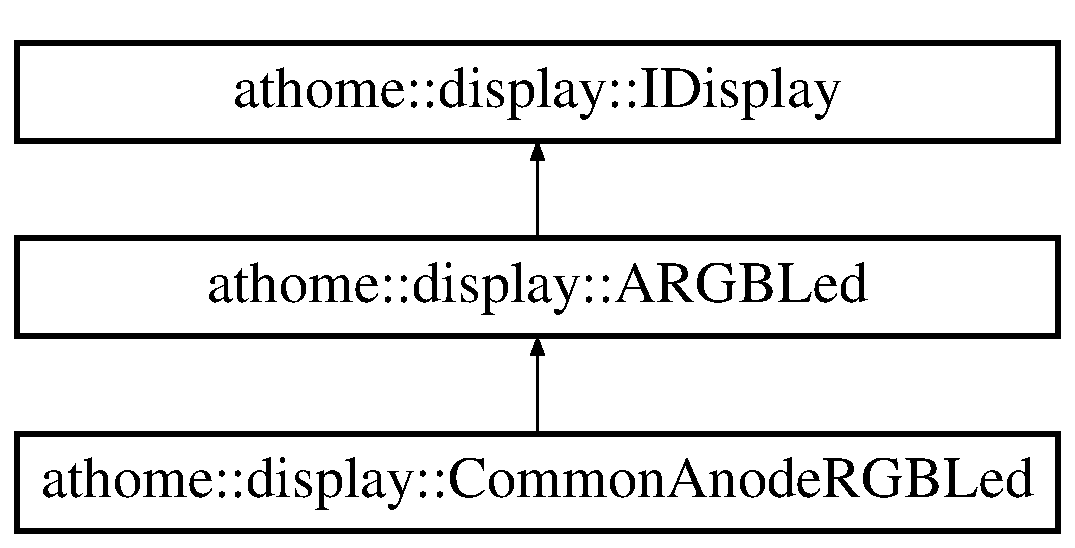
\includegraphics[height=3.000000cm]{classathome_1_1display_1_1_common_anode_r_g_b_led}
\end{center}
\end{figure}
\subsection*{Public Member Functions}
\begin{DoxyCompactItemize}
\item 
\mbox{\Hypertarget{classathome_1_1display_1_1_common_anode_r_g_b_led_a3695455b373a3ec0f7bb0ea76eee6e36}\label{classathome_1_1display_1_1_common_anode_r_g_b_led_a3695455b373a3ec0f7bb0ea76eee6e36}} 
{\bfseries Common\+Anode\+R\+G\+B\+Led} (uint8\+\_\+t, uint8\+\_\+t, uint8\+\_\+t)
\item 
\mbox{\Hypertarget{classathome_1_1display_1_1_common_anode_r_g_b_led_a79535998b06fdc7046bf8006ad1e3eb6}\label{classathome_1_1display_1_1_common_anode_r_g_b_led_a79535998b06fdc7046bf8006ad1e3eb6}} 
{\bfseries Common\+Anode\+R\+G\+B\+Led} (const \mbox{\hyperlink{classathome_1_1display_1_1_common_anode_r_g_b_led}{Common\+Anode\+R\+G\+B\+Led}} \&)=delete
\item 
\mbox{\Hypertarget{classathome_1_1display_1_1_common_anode_r_g_b_led_a59e331dcbb1d7b028b932148c30f000f}\label{classathome_1_1display_1_1_common_anode_r_g_b_led_a59e331dcbb1d7b028b932148c30f000f}} 
\mbox{\hyperlink{classathome_1_1display_1_1_common_anode_r_g_b_led}{Common\+Anode\+R\+G\+B\+Led}} \& {\bfseries operator=} (const \mbox{\hyperlink{classathome_1_1display_1_1_common_anode_r_g_b_led}{Common\+Anode\+R\+G\+B\+Led}} \&)
\item 
void \mbox{\hyperlink{classathome_1_1display_1_1_common_anode_r_g_b_led_ab7daf7dcc6ac1e3fcab202cae484b237}{update}} ()
\end{DoxyCompactItemize}


\subsection{Member Function Documentation}
\mbox{\Hypertarget{classathome_1_1display_1_1_common_anode_r_g_b_led_ab7daf7dcc6ac1e3fcab202cae484b237}\label{classathome_1_1display_1_1_common_anode_r_g_b_led_ab7daf7dcc6ac1e3fcab202cae484b237}} 
\index{athome\+::display\+::\+Common\+Anode\+R\+G\+B\+Led@{athome\+::display\+::\+Common\+Anode\+R\+G\+B\+Led}!update@{update}}
\index{update@{update}!athome\+::display\+::\+Common\+Anode\+R\+G\+B\+Led@{athome\+::display\+::\+Common\+Anode\+R\+G\+B\+Led}}
\subsubsection{\texorpdfstring{update()}{update()}}
{\footnotesize\ttfamily void athome\+::display\+::\+Common\+Anode\+R\+G\+B\+Led\+::update (\begin{DoxyParamCaption}{ }\end{DoxyParamCaption})\hspace{0.3cm}{\ttfamily [virtual]}}

Update display content 

Implements \mbox{\hyperlink{classathome_1_1display_1_1_a_r_g_b_led_a725ceca0c01735daa9c95148baf075ab}{athome\+::display\+::\+A\+R\+G\+B\+Led}}.



The documentation for this class was generated from the following files\+:\begin{DoxyCompactItemize}
\item 
src/Common\+Anode\+R\+G\+B\+Led.\+hpp\item 
src/display/Common\+Anode\+R\+G\+B\+Led.\+cpp\end{DoxyCompactItemize}

\hypertarget{classathome_1_1display_1_1_common_cathode_r_g_b_led}{}\section{athome\+:\+:display\+:\+:Common\+Cathode\+R\+G\+B\+Led Class Reference}
\label{classathome_1_1display_1_1_common_cathode_r_g_b_led}\index{athome\+::display\+::\+Common\+Cathode\+R\+G\+B\+Led@{athome\+::display\+::\+Common\+Cathode\+R\+G\+B\+Led}}
Inheritance diagram for athome\+:\+:display\+:\+:Common\+Cathode\+R\+G\+B\+Led\+:\begin{figure}[H]
\begin{center}
\leavevmode
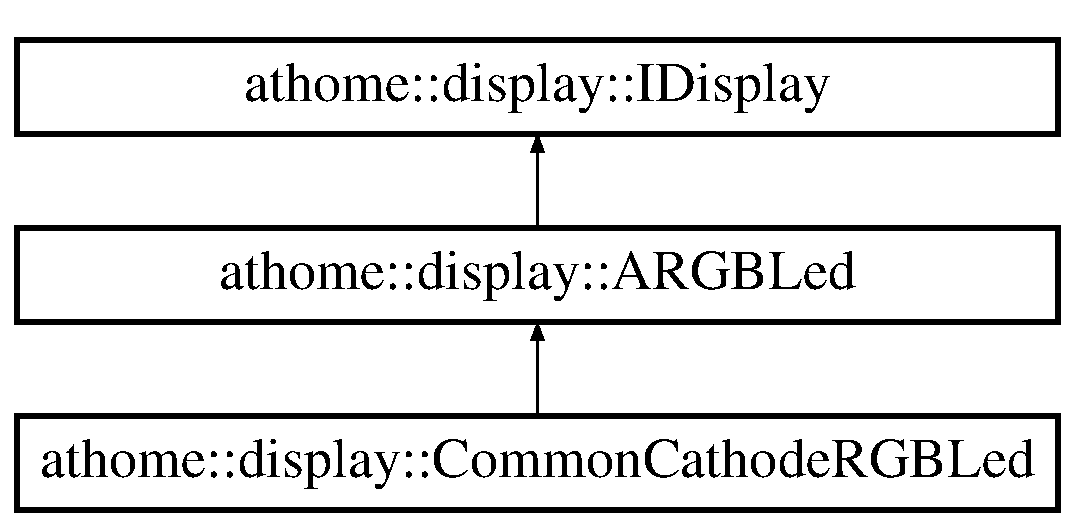
\includegraphics[height=3.000000cm]{classathome_1_1display_1_1_common_cathode_r_g_b_led}
\end{center}
\end{figure}
\subsection*{Public Member Functions}
\begin{DoxyCompactItemize}
\item 
\mbox{\Hypertarget{classathome_1_1display_1_1_common_cathode_r_g_b_led_a4449607163d583410574fc7c138b012b}\label{classathome_1_1display_1_1_common_cathode_r_g_b_led_a4449607163d583410574fc7c138b012b}} 
{\bfseries Common\+Cathode\+R\+G\+B\+Led} (uint8\+\_\+t, uint8\+\_\+t, uint8\+\_\+t)
\item 
\mbox{\Hypertarget{classathome_1_1display_1_1_common_cathode_r_g_b_led_aaf13aacaf891bb7594cf6994018c1b4a}\label{classathome_1_1display_1_1_common_cathode_r_g_b_led_aaf13aacaf891bb7594cf6994018c1b4a}} 
{\bfseries Common\+Cathode\+R\+G\+B\+Led} (const \mbox{\hyperlink{classathome_1_1display_1_1_common_cathode_r_g_b_led}{Common\+Cathode\+R\+G\+B\+Led}} \&)=delete
\item 
\mbox{\Hypertarget{classathome_1_1display_1_1_common_cathode_r_g_b_led_a700bea6a579e9c89aac93610671d47a4}\label{classathome_1_1display_1_1_common_cathode_r_g_b_led_a700bea6a579e9c89aac93610671d47a4}} 
\mbox{\hyperlink{classathome_1_1display_1_1_common_cathode_r_g_b_led}{Common\+Cathode\+R\+G\+B\+Led}} \& {\bfseries operator=} (const \mbox{\hyperlink{classathome_1_1display_1_1_common_cathode_r_g_b_led}{Common\+Cathode\+R\+G\+B\+Led}} \&)
\item 
void \mbox{\hyperlink{classathome_1_1display_1_1_common_cathode_r_g_b_led_ab78ab6aef619d8e0941dd11d4cfbb545}{update}} ()
\end{DoxyCompactItemize}


\subsection{Member Function Documentation}
\mbox{\Hypertarget{classathome_1_1display_1_1_common_cathode_r_g_b_led_ab78ab6aef619d8e0941dd11d4cfbb545}\label{classathome_1_1display_1_1_common_cathode_r_g_b_led_ab78ab6aef619d8e0941dd11d4cfbb545}} 
\index{athome\+::display\+::\+Common\+Cathode\+R\+G\+B\+Led@{athome\+::display\+::\+Common\+Cathode\+R\+G\+B\+Led}!update@{update}}
\index{update@{update}!athome\+::display\+::\+Common\+Cathode\+R\+G\+B\+Led@{athome\+::display\+::\+Common\+Cathode\+R\+G\+B\+Led}}
\subsubsection{\texorpdfstring{update()}{update()}}
{\footnotesize\ttfamily void athome\+::display\+::\+Common\+Cathode\+R\+G\+B\+Led\+::update (\begin{DoxyParamCaption}{ }\end{DoxyParamCaption})\hspace{0.3cm}{\ttfamily [virtual]}}

Update display content 

Implements \mbox{\hyperlink{classathome_1_1display_1_1_a_r_g_b_led_a725ceca0c01735daa9c95148baf075ab}{athome\+::display\+::\+A\+R\+G\+B\+Led}}.



The documentation for this class was generated from the following files\+:\begin{DoxyCompactItemize}
\item 
src/Common\+Cathode\+R\+G\+B\+Led.\+hpp\item 
src/display/Common\+Cathode\+R\+G\+B\+Led.\+cpp\end{DoxyCompactItemize}

\hypertarget{classathome_1_1time_1_1_i_time_1_1_date_time}{}\section{athome\+:\+:time\+:\+:I\+Time\+:\+:Date\+Time Class Reference}
\label{classathome_1_1time_1_1_i_time_1_1_date_time}\index{athome\+::time\+::\+I\+Time\+::\+Date\+Time@{athome\+::time\+::\+I\+Time\+::\+Date\+Time}}
Inheritance diagram for athome\+:\+:time\+:\+:I\+Time\+:\+:Date\+Time\+:\begin{figure}[H]
\begin{center}
\leavevmode
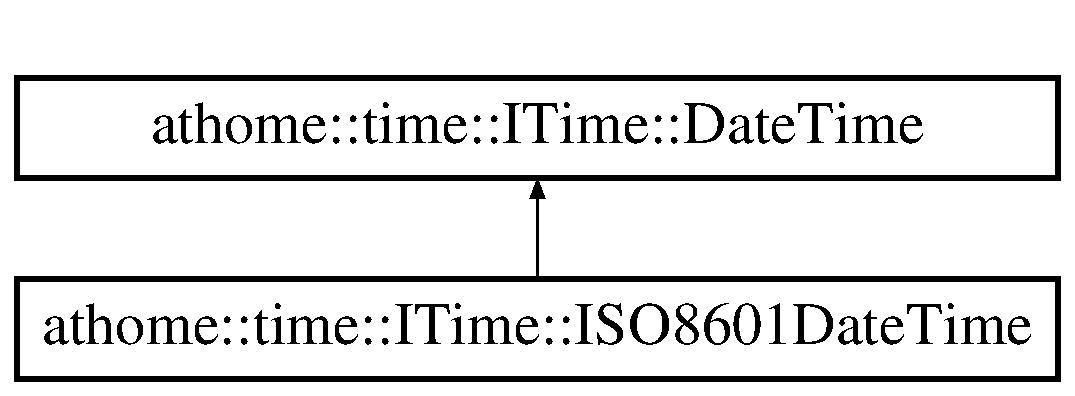
\includegraphics[height=2.000000cm]{classathome_1_1time_1_1_i_time_1_1_date_time}
\end{center}
\end{figure}
\subsection*{Public Member Functions}
\begin{DoxyCompactItemize}
\item 
\mbox{\Hypertarget{classathome_1_1time_1_1_i_time_1_1_date_time_a0380ffd91df34e5f59f7e24a0d31690e}\label{classathome_1_1time_1_1_i_time_1_1_date_time_a0380ffd91df34e5f59f7e24a0d31690e}} 
\mbox{\hyperlink{classathome_1_1time_1_1_i_time_1_1_date_time}{Date\+Time}} \& {\bfseries operator=} (const \mbox{\hyperlink{classathome_1_1time_1_1_i_time_1_1_date_time}{Date\+Time}} \&date)
\end{DoxyCompactItemize}
\subsection*{Public Attributes}
\begin{DoxyCompactItemize}
\item 
\mbox{\Hypertarget{classathome_1_1time_1_1_i_time_1_1_date_time_aa8d293191e225992f76d54a20bf20c4c}\label{classathome_1_1time_1_1_i_time_1_1_date_time_aa8d293191e225992f76d54a20bf20c4c}} 
uint32\+\_\+t {\bfseries second}\+: 6
\item 
\mbox{\Hypertarget{classathome_1_1time_1_1_i_time_1_1_date_time_aeaf95ec7b94f3515f1351ace98abacde}\label{classathome_1_1time_1_1_i_time_1_1_date_time_aeaf95ec7b94f3515f1351ace98abacde}} 
uint32\+\_\+t {\bfseries minute}\+: 6
\item 
\mbox{\Hypertarget{classathome_1_1time_1_1_i_time_1_1_date_time_a3ca068c42464b2aedf8ad38fbf04a706}\label{classathome_1_1time_1_1_i_time_1_1_date_time_a3ca068c42464b2aedf8ad38fbf04a706}} 
uint32\+\_\+t {\bfseries hour}\+: 5
\item 
\mbox{\Hypertarget{classathome_1_1time_1_1_i_time_1_1_date_time_a2c1e84fc382eba06a6271f66c2f7ca0b}\label{classathome_1_1time_1_1_i_time_1_1_date_time_a2c1e84fc382eba06a6271f66c2f7ca0b}} 
uint32\+\_\+t {\bfseries day}\+: 5
\item 
\mbox{\Hypertarget{classathome_1_1time_1_1_i_time_1_1_date_time_a2bf001a7e2b93e0b0077dca04ef8a60d}\label{classathome_1_1time_1_1_i_time_1_1_date_time_a2bf001a7e2b93e0b0077dca04ef8a60d}} 
uint32\+\_\+t {\bfseries month}\+: 4
\item 
\mbox{\Hypertarget{classathome_1_1time_1_1_i_time_1_1_date_time_a7331035799fc6b1c66c61cbbcbfbeb1e}\label{classathome_1_1time_1_1_i_time_1_1_date_time_a7331035799fc6b1c66c61cbbcbfbeb1e}} 
uint32\+\_\+t {\bfseries year}\+: 6
\end{DoxyCompactItemize}


The documentation for this class was generated from the following file\+:\begin{DoxyCompactItemize}
\item 
src/I\+Time.\+hpp\end{DoxyCompactItemize}

\hypertarget{classathome_1_1time_1_1_d_s1307}{}\section{athome\+:\+:time\+:\+:D\+S1307 Class Reference}
\label{classathome_1_1time_1_1_d_s1307}\index{athome\+::time\+::\+D\+S1307@{athome\+::time\+::\+D\+S1307}}
Inheritance diagram for athome\+:\+:time\+:\+:D\+S1307\+:\begin{figure}[H]
\begin{center}
\leavevmode
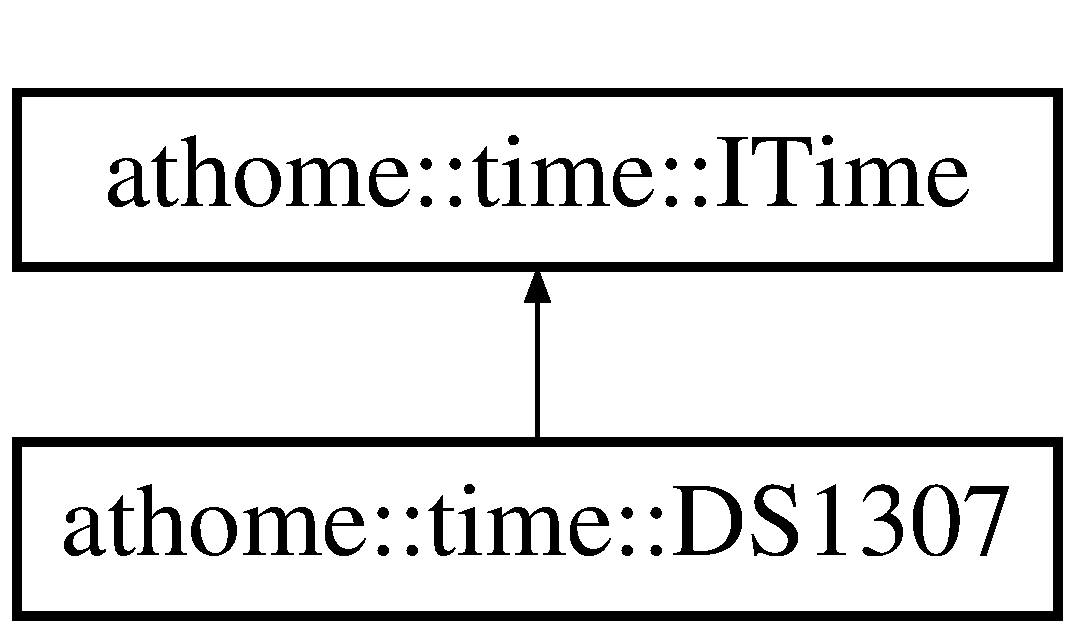
\includegraphics[height=2.000000cm]{classathome_1_1time_1_1_d_s1307}
\end{center}
\end{figure}
\subsection*{Public Member Functions}
\begin{DoxyCompactItemize}
\item 
\mbox{\Hypertarget{classathome_1_1time_1_1_d_s1307_ac9894245cf5bef539272e6ed6c5ed237}\label{classathome_1_1time_1_1_d_s1307_ac9894245cf5bef539272e6ed6c5ed237}} 
{\bfseries D\+S1307} (Two\+Wire \&)
\item 
\mbox{\Hypertarget{classathome_1_1time_1_1_d_s1307_a28a802496d0d76cac3232720c0a1243e}\label{classathome_1_1time_1_1_d_s1307_a28a802496d0d76cac3232720c0a1243e}} 
{\bfseries D\+S1307} (const \mbox{\hyperlink{classathome_1_1time_1_1_d_s1307}{D\+S1307}} \&)=delete
\item 
\mbox{\Hypertarget{classathome_1_1time_1_1_d_s1307_a6aabfb829a3ac526526348d22180e09c}\label{classathome_1_1time_1_1_d_s1307_a6aabfb829a3ac526526348d22180e09c}} 
\mbox{\hyperlink{classathome_1_1time_1_1_d_s1307}{D\+S1307}} \& {\bfseries operator=} (const \mbox{\hyperlink{classathome_1_1time_1_1_d_s1307}{D\+S1307}} \&)=delete
\item 
\mbox{\Hypertarget{classathome_1_1time_1_1_d_s1307_aa9c452a50a12e67f92346ce3f770d283}\label{classathome_1_1time_1_1_d_s1307_aa9c452a50a12e67f92346ce3f770d283}} 
virtual const \mbox{\hyperlink{structathome_1_1time_1_1_i_time_1_1_i_s_o8601_date_time}{I\+Time\+::\+I\+S\+O8601\+Date\+Time}} \& {\bfseries get\+Date\+Time} ()
\item 
\mbox{\Hypertarget{classathome_1_1time_1_1_d_s1307_a595285f3bf325d2208c6d48b686c5b86}\label{classathome_1_1time_1_1_d_s1307_a595285f3bf325d2208c6d48b686c5b86}} 
virtual void {\bfseries set\+Current\+Date\+Time} (const \mbox{\hyperlink{classathome_1_1time_1_1_i_time_1_1_date_time}{Date\+Time}} \&)
\end{DoxyCompactItemize}
\subsection*{Protected Member Functions}
\begin{DoxyCompactItemize}
\item 
\mbox{\Hypertarget{classathome_1_1time_1_1_d_s1307_a8050ac76655291bfe8ada1374044975e}\label{classathome_1_1time_1_1_d_s1307_a8050ac76655291bfe8ada1374044975e}} 
void {\bfseries setup} ()
\item 
\mbox{\Hypertarget{classathome_1_1time_1_1_d_s1307_a1ba76f50a478dd94d64048ede8af5c45}\label{classathome_1_1time_1_1_d_s1307_a1ba76f50a478dd94d64048ede8af5c45}} 
bool {\bfseries is\+\_\+running} ()
\item 
\mbox{\Hypertarget{classathome_1_1time_1_1_d_s1307_afbf8528f8ceec1fd3dde59c470c6605e}\label{classathome_1_1time_1_1_d_s1307_afbf8528f8ceec1fd3dde59c470c6605e}} 
uint8\+\_\+t {\bfseries bcd2bin} (uint8\+\_\+t)
\item 
\mbox{\Hypertarget{classathome_1_1time_1_1_d_s1307_abbd3c6698cc2a6c70be1d543fb36853b}\label{classathome_1_1time_1_1_d_s1307_abbd3c6698cc2a6c70be1d543fb36853b}} 
uint8\+\_\+t {\bfseries bin2bcd} (uint8\+\_\+t)
\end{DoxyCompactItemize}


The documentation for this class was generated from the following files\+:\begin{DoxyCompactItemize}
\item 
src/D\+S1307.\+hpp\item 
src/time/D\+S1307.\+cpp\end{DoxyCompactItemize}

\hypertarget{classathome_1_1sensor_1_1_dummy_sensor}{}\section{athome\+:\+:sensor\+:\+:Dummy\+Sensor$<$ T, U, limit $>$ Class Template Reference}
\label{classathome_1_1sensor_1_1_dummy_sensor}\index{athome\+::sensor\+::\+Dummy\+Sensor$<$ T, U, limit $>$@{athome\+::sensor\+::\+Dummy\+Sensor$<$ T, U, limit $>$}}
Inheritance diagram for athome\+:\+:sensor\+:\+:Dummy\+Sensor$<$ T, U, limit $>$\+:\begin{figure}[H]
\begin{center}
\leavevmode
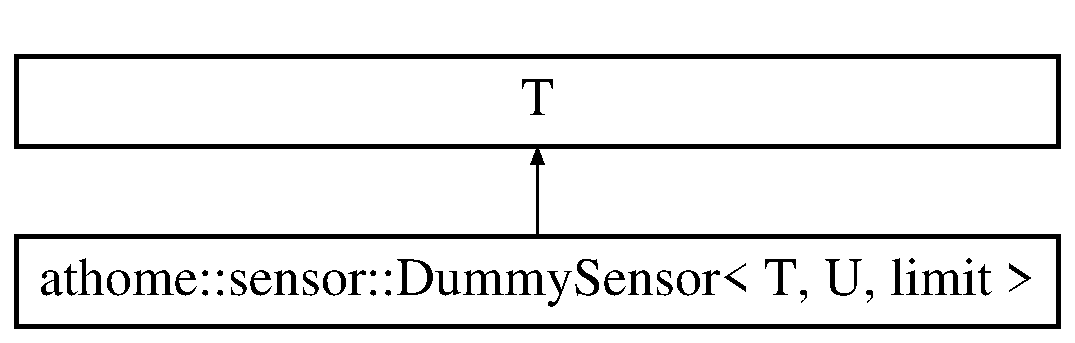
\includegraphics[height=2.000000cm]{classathome_1_1sensor_1_1_dummy_sensor}
\end{center}
\end{figure}
\subsection*{Public Member Functions}
\begin{DoxyCompactItemize}
\item 
\mbox{\Hypertarget{classathome_1_1sensor_1_1_dummy_sensor_ac9ac77587454246fb4f1f79010262a27}\label{classathome_1_1sensor_1_1_dummy_sensor_ac9ac77587454246fb4f1f79010262a27}} 
{\bfseries Dummy\+Sensor} (const \mbox{\hyperlink{classathome_1_1sensor_1_1_dummy_sensor}{Dummy\+Sensor}} \&)=delete
\item 
\mbox{\Hypertarget{classathome_1_1sensor_1_1_dummy_sensor_a65546910321b5bbbf00b12069ee484ee}\label{classathome_1_1sensor_1_1_dummy_sensor_a65546910321b5bbbf00b12069ee484ee}} 
\mbox{\hyperlink{classathome_1_1sensor_1_1_dummy_sensor}{Dummy\+Sensor}} \& {\bfseries operator=} (const \mbox{\hyperlink{classathome_1_1sensor_1_1_dummy_sensor}{Dummy\+Sensor}} \&)=delete
\item 
\mbox{\Hypertarget{classathome_1_1sensor_1_1_dummy_sensor_ab01a87f5dfa35297adf55ecefe407ba4}\label{classathome_1_1sensor_1_1_dummy_sensor_ab01a87f5dfa35297adf55ecefe407ba4}} 
virtual U {\bfseries get\+Sensor\+Sample} ()
\end{DoxyCompactItemize}


The documentation for this class was generated from the following file\+:\begin{DoxyCompactItemize}
\item 
src/Dummy\+Sensor.\+hpp\end{DoxyCompactItemize}

\hypertarget{classathome_1_1communication_1_1wifi_1_1_e_s_p8266_wi_fi_communicator}{}\section{athome\+:\+:communication\+:\+:wifi\+:\+:E\+S\+P8266\+Wi\+Fi\+Communicator Class Reference}
\label{classathome_1_1communication_1_1wifi_1_1_e_s_p8266_wi_fi_communicator}\index{athome\+::communication\+::wifi\+::\+E\+S\+P8266\+Wi\+Fi\+Communicator@{athome\+::communication\+::wifi\+::\+E\+S\+P8266\+Wi\+Fi\+Communicator}}
Inheritance diagram for athome\+:\+:communication\+:\+:wifi\+:\+:E\+S\+P8266\+Wi\+Fi\+Communicator\+:\begin{figure}[H]
\begin{center}
\leavevmode
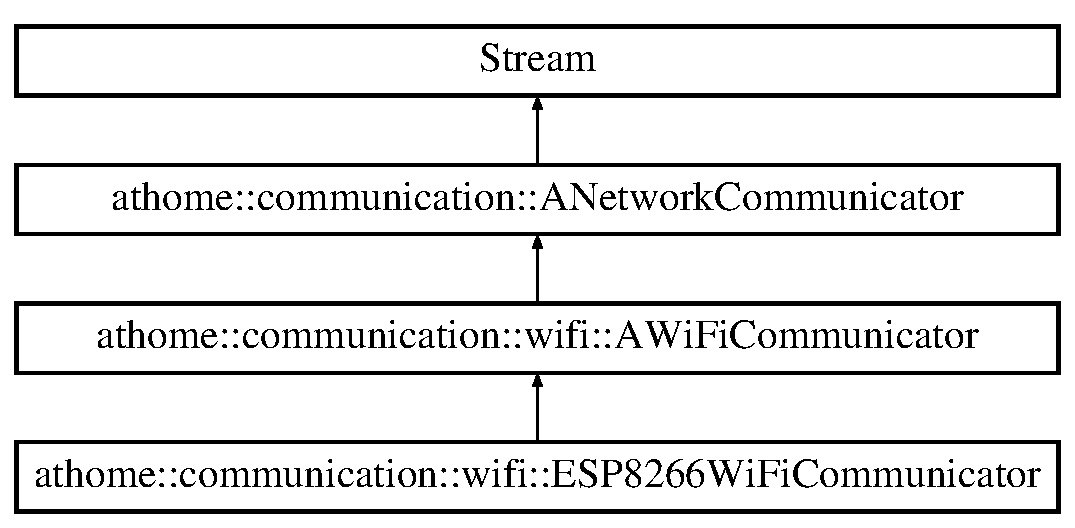
\includegraphics[height=4.000000cm]{classathome_1_1communication_1_1wifi_1_1_e_s_p8266_wi_fi_communicator}
\end{center}
\end{figure}
\subsection*{Public Member Functions}
\begin{DoxyCompactItemize}
\item 
\mbox{\Hypertarget{classathome_1_1communication_1_1wifi_1_1_e_s_p8266_wi_fi_communicator_a243e2a1e06278152e9b05b171d4fa14e}\label{classathome_1_1communication_1_1wifi_1_1_e_s_p8266_wi_fi_communicator_a243e2a1e06278152e9b05b171d4fa14e}} 
{\bfseries E\+S\+P8266\+Wi\+Fi\+Communicator} (int, int)
\item 
\mbox{\Hypertarget{classathome_1_1communication_1_1wifi_1_1_e_s_p8266_wi_fi_communicator_a494ac790093af57da729cef136adf0b2}\label{classathome_1_1communication_1_1wifi_1_1_e_s_p8266_wi_fi_communicator_a494ac790093af57da729cef136adf0b2}} 
{\bfseries E\+S\+P8266\+Wi\+Fi\+Communicator} (const \mbox{\hyperlink{classathome_1_1communication_1_1wifi_1_1_e_s_p8266_wi_fi_communicator}{E\+S\+P8266\+Wi\+Fi\+Communicator}} \&)=delete
\item 
\mbox{\Hypertarget{classathome_1_1communication_1_1wifi_1_1_e_s_p8266_wi_fi_communicator_a7c880abd129da8dc00cd82696e4034e3}\label{classathome_1_1communication_1_1wifi_1_1_e_s_p8266_wi_fi_communicator_a7c880abd129da8dc00cd82696e4034e3}} 
\mbox{\hyperlink{classathome_1_1communication_1_1wifi_1_1_e_s_p8266_wi_fi_communicator}{E\+S\+P8266\+Wi\+Fi\+Communicator}} \& {\bfseries operator=} (const \mbox{\hyperlink{classathome_1_1communication_1_1wifi_1_1_e_s_p8266_wi_fi_communicator}{E\+S\+P8266\+Wi\+Fi\+Communicator}} \&)=delete
\item 
virtual int \mbox{\hyperlink{classathome_1_1communication_1_1wifi_1_1_e_s_p8266_wi_fi_communicator_af9b1e28910959893748763faaa5373a0}{available}} ()
\item 
virtual int \mbox{\hyperlink{classathome_1_1communication_1_1wifi_1_1_e_s_p8266_wi_fi_communicator_a1cadc570e912c164279ef0ebc5b178a5}{read}} ()
\item 
virtual int \mbox{\hyperlink{classathome_1_1communication_1_1wifi_1_1_e_s_p8266_wi_fi_communicator_affeb5491ad5c97fa53a683926f8184d2}{peek}} ()
\item 
virtual size\+\_\+t \mbox{\hyperlink{classathome_1_1communication_1_1wifi_1_1_e_s_p8266_wi_fi_communicator_afd3c1c4ce7d68717a7bb2cf1b9dc962f}{write}} (uint8\+\_\+t)
\item 
virtual void \mbox{\hyperlink{classathome_1_1communication_1_1wifi_1_1_e_s_p8266_wi_fi_communicator_af95ca7f47285b13fc895e0d9323ee320}{flush}} ()
\item 
\mbox{\Hypertarget{classathome_1_1communication_1_1wifi_1_1_e_s_p8266_wi_fi_communicator_af51040a77a72236bac1b7da51a609506}\label{classathome_1_1communication_1_1wifi_1_1_e_s_p8266_wi_fi_communicator_af51040a77a72236bac1b7da51a609506}} 
void {\bfseries enable} ()
\item 
\mbox{\Hypertarget{classathome_1_1communication_1_1wifi_1_1_e_s_p8266_wi_fi_communicator_a5f78b62392cf22fe115baaa7adaa37f2}\label{classathome_1_1communication_1_1wifi_1_1_e_s_p8266_wi_fi_communicator_a5f78b62392cf22fe115baaa7adaa37f2}} 
void {\bfseries disable} ()
\item 
virtual int \mbox{\hyperlink{classathome_1_1communication_1_1wifi_1_1_e_s_p8266_wi_fi_communicator_a58cc439be2f368b346bbbe1601a9b675}{connect}} ()
\item 
virtual int \mbox{\hyperlink{classathome_1_1communication_1_1wifi_1_1_e_s_p8266_wi_fi_communicator_a7e53e10b858aebc5e7c6c0ea6007f84a}{disconnect}} ()
\item 
virtual int \mbox{\hyperlink{classathome_1_1communication_1_1wifi_1_1_e_s_p8266_wi_fi_communicator_a159a93b350df135daa967665c9e53e2f}{connect\+To\+Host}} ()
\item 
virtual int \mbox{\hyperlink{classathome_1_1communication_1_1wifi_1_1_e_s_p8266_wi_fi_communicator_a0f8adbe1b1d219148c4f340980056356}{disconnect\+From\+Host}} ()
\item 
virtual bool \mbox{\hyperlink{classathome_1_1communication_1_1wifi_1_1_e_s_p8266_wi_fi_communicator_aefadac9b1a67d52853495dfabecad5fd}{is\+Connected}} () const
\end{DoxyCompactItemize}
\subsection*{Additional Inherited Members}


\subsection{Member Function Documentation}
\mbox{\Hypertarget{classathome_1_1communication_1_1wifi_1_1_e_s_p8266_wi_fi_communicator_af9b1e28910959893748763faaa5373a0}\label{classathome_1_1communication_1_1wifi_1_1_e_s_p8266_wi_fi_communicator_af9b1e28910959893748763faaa5373a0}} 
\index{athome\+::communication\+::wifi\+::\+E\+S\+P8266\+Wi\+Fi\+Communicator@{athome\+::communication\+::wifi\+::\+E\+S\+P8266\+Wi\+Fi\+Communicator}!available@{available}}
\index{available@{available}!athome\+::communication\+::wifi\+::\+E\+S\+P8266\+Wi\+Fi\+Communicator@{athome\+::communication\+::wifi\+::\+E\+S\+P8266\+Wi\+Fi\+Communicator}}
\subsubsection{\texorpdfstring{available()}{available()}}
{\footnotesize\ttfamily int athome\+::communication\+::wifi\+::\+E\+S\+P8266\+Wi\+Fi\+Communicator\+::available (\begin{DoxyParamCaption}{ }\end{DoxyParamCaption})\hspace{0.3cm}{\ttfamily [virtual]}}

Virtual method inherited from Stream interface. \mbox{[}See documentation on Arduino reference.\mbox{]}(\href{https://www.arduino.cc/reference/en/language/functions/communication/stream/streamavailable/}{\tt https\+://www.\+arduino.\+cc/reference/en/language/functions/communication/stream/streamavailable/}) 

Implements \mbox{\hyperlink{classathome_1_1communication_1_1_a_network_communicator_a2bf367d03c98e8523fda71dd43ffa2fb}{athome\+::communication\+::\+A\+Network\+Communicator}}.

\mbox{\Hypertarget{classathome_1_1communication_1_1wifi_1_1_e_s_p8266_wi_fi_communicator_a58cc439be2f368b346bbbe1601a9b675}\label{classathome_1_1communication_1_1wifi_1_1_e_s_p8266_wi_fi_communicator_a58cc439be2f368b346bbbe1601a9b675}} 
\index{athome\+::communication\+::wifi\+::\+E\+S\+P8266\+Wi\+Fi\+Communicator@{athome\+::communication\+::wifi\+::\+E\+S\+P8266\+Wi\+Fi\+Communicator}!connect@{connect}}
\index{connect@{connect}!athome\+::communication\+::wifi\+::\+E\+S\+P8266\+Wi\+Fi\+Communicator@{athome\+::communication\+::wifi\+::\+E\+S\+P8266\+Wi\+Fi\+Communicator}}
\subsubsection{\texorpdfstring{connect()}{connect()}}
{\footnotesize\ttfamily int athome\+::communication\+::wifi\+::\+E\+S\+P8266\+Wi\+Fi\+Communicator\+::connect (\begin{DoxyParamCaption}{ }\end{DoxyParamCaption})\hspace{0.3cm}{\ttfamily [virtual]}}

Virtual method used to implement connection to Wi\+Fi network through the adapter.

A return value of 0 is expected to indicate the connection was successful, otherwise all other values are available for error codes.

Example\+:


\begin{DoxyCode}
\textcolor{preprocessor}{#include <string.h>}
\textcolor{preprocessor}{#include <AtHome.h>}

\textcolor{keyword}{using} \mbox{\hyperlink{structathome_1_1communication_1_1wifi_1_1s__wifi__access__point}{athome::communication::wifi::WiFi\_ap}}; \textcolor{comment}{// Use this to not have to}
\mbox{\hyperlink{classathome_1_1communication_1_1wifi_1_1_e_s_p8266_wi_fi_communicator_afd3c1c4ce7d68717a7bb2cf1b9dc962f}{write}} the full \textcolor{keyword}{namespace }names further using
\mbox{\hyperlink{namespaceathome}{athome}}::communication::wifi::AWiFiCommunicator;

void my\_function\_connecting\_wifi\_to\_network\_called\_foobar(AWiFiCommunicator
&wifi) \{ WiFi\_ap network; \textcolor{comment}{// Declare a WiFi\_ap structure}
  strncpy(network.ssid, \textcolor{stringliteral}{"foobar"}, \textcolor{keyword}{sizeof}(network.ssid)); \textcolor{comment}{// Copy "foobar"}
in the ssid field of the structure, as the SSID of a WiFi network is the
name shown to humans strncpy(network.password, \textcolor{stringliteral}{"12345678"},
\textcolor{keyword}{sizeof}(network.password)); \textcolor{comment}{// Copy "12345678" in the password field, to set}
the password used by the WiFi network wifi.setAccessPoint(network); \textcolor{comment}{// Set}
the WiFi network parameters we created \textcolor{keywordflow}{if} (!wifi.connect()) \{ \textcolor{comment}{// Connect to}
\textcolor{keyword}{this} network Serial.println(\textcolor{stringliteral}{"Successfully connected to WiFi network"}); \}
\textcolor{keywordflow}{else} \{ Serial.println(\textcolor{stringliteral}{"Connection to WiFi network failed"});
  \}
\}
\end{DoxyCode}
 

Implements \mbox{\hyperlink{classathome_1_1communication_1_1wifi_1_1_a_wi_fi_communicator_a309927109fbc19aa0fb2afb71d50bbf9}{athome\+::communication\+::wifi\+::\+A\+Wi\+Fi\+Communicator}}.

\mbox{\Hypertarget{classathome_1_1communication_1_1wifi_1_1_e_s_p8266_wi_fi_communicator_a159a93b350df135daa967665c9e53e2f}\label{classathome_1_1communication_1_1wifi_1_1_e_s_p8266_wi_fi_communicator_a159a93b350df135daa967665c9e53e2f}} 
\index{athome\+::communication\+::wifi\+::\+E\+S\+P8266\+Wi\+Fi\+Communicator@{athome\+::communication\+::wifi\+::\+E\+S\+P8266\+Wi\+Fi\+Communicator}!connect\+To\+Host@{connect\+To\+Host}}
\index{connect\+To\+Host@{connect\+To\+Host}!athome\+::communication\+::wifi\+::\+E\+S\+P8266\+Wi\+Fi\+Communicator@{athome\+::communication\+::wifi\+::\+E\+S\+P8266\+Wi\+Fi\+Communicator}}
\subsubsection{\texorpdfstring{connect\+To\+Host()}{connectToHost()}}
{\footnotesize\ttfamily int athome\+::communication\+::wifi\+::\+E\+S\+P8266\+Wi\+Fi\+Communicator\+::connect\+To\+Host (\begin{DoxyParamCaption}{ }\end{DoxyParamCaption})\hspace{0.3cm}{\ttfamily [virtual]}}

Virtual method used to connect adapter to a socket on a host.

A return value of 0 is expected to indicate success, otherwise all other values are available for error codes.

Example\+:


\begin{DoxyCode}
\textcolor{preprocessor}{#include <AtHome.h>}

\textcolor{keyword}{using} \mbox{\hyperlink{structathome_1_1communication_1_1ip_1_1s__host}{athome::communication::ip::tcp\_host}}; \textcolor{comment}{// Use this to not have to
       write}
the full \textcolor{keyword}{namespace }names further using
\mbox{\hyperlink{namespaceathome}{athome}}::communication::wifi::WiFi\_client; using
\mbox{\hyperlink{classathome_1_1communication_1_1wifi_1_1_a_wi_fi_communicator}{athome::communication::wifi::AWiFiCommunicator}};

void my\_function\_connecting\_to\_http\_port\_on\_router(AWiFiCommunicator &wifi)
\{ \textcolor{keyword}{const} WiFi\_client &my\_ip = wifi.getConnectionAddresses(); \textcolor{comment}{// Get our}
actual MAC and IP (IPv4 or IPv6) addresses tcp\_host router =
\{\{my\_ip.ipv4[0], my\_ip.ipv4[1], my\_ip.ipv4[2], 1\}, 80\}; \textcolor{comment}{// Use our current}
IPv4 address to deduce the one of the router, which often is the same as
ours but ending with the value 1 wifi.setHost(router); \textcolor{comment}{// Set the new host}
to \mbox{\hyperlink{classathome_1_1communication_1_1wifi_1_1_e_s_p8266_wi_fi_communicator_a58cc439be2f368b346bbbe1601a9b675}{connect}} on, our structure tcp\_host is a couple IP + port \textcolor{keywordflow}{if}
(!wifi.connectToHost()) \{ \textcolor{comment}{// Connect to the socket on the host}
    Serial.println(\textcolor{stringliteral}{"Successfully connected to host"});
  \} \textcolor{keywordflow}{else} \{
    Serial.println(\textcolor{stringliteral}{"Failed to connect to host"});
  \}
\}
\end{DoxyCode}
 

Implements \mbox{\hyperlink{classathome_1_1communication_1_1_a_network_communicator_a370176dae8f38225446e83a132dbcff7}{athome\+::communication\+::\+A\+Network\+Communicator}}.

\mbox{\Hypertarget{classathome_1_1communication_1_1wifi_1_1_e_s_p8266_wi_fi_communicator_a7e53e10b858aebc5e7c6c0ea6007f84a}\label{classathome_1_1communication_1_1wifi_1_1_e_s_p8266_wi_fi_communicator_a7e53e10b858aebc5e7c6c0ea6007f84a}} 
\index{athome\+::communication\+::wifi\+::\+E\+S\+P8266\+Wi\+Fi\+Communicator@{athome\+::communication\+::wifi\+::\+E\+S\+P8266\+Wi\+Fi\+Communicator}!disconnect@{disconnect}}
\index{disconnect@{disconnect}!athome\+::communication\+::wifi\+::\+E\+S\+P8266\+Wi\+Fi\+Communicator@{athome\+::communication\+::wifi\+::\+E\+S\+P8266\+Wi\+Fi\+Communicator}}
\subsubsection{\texorpdfstring{disconnect()}{disconnect()}}
{\footnotesize\ttfamily int athome\+::communication\+::wifi\+::\+E\+S\+P8266\+Wi\+Fi\+Communicator\+::disconnect (\begin{DoxyParamCaption}{ }\end{DoxyParamCaption})\hspace{0.3cm}{\ttfamily [virtual]}}

Virtual method used to implement disconnection of the current Wi\+Fi network through the adapter.

A return value of 0 is expected to indicate success, otherwise all other values are available for error codes.

Usage is as simple as this\+:


\begin{DoxyCode}
\textcolor{preprocessor}{#include <AWiFiCommunicator.hpp>}

\textcolor{keyword}{using} \mbox{\hyperlink{classathome_1_1communication_1_1wifi_1_1_a_wi_fi_communicator}{athome::communication::wifi::AWiFiCommunicator}};

\textcolor{keywordtype}{void} my\_function\_disconnecting\_wifi\_adapters(AWiFiCommuncator &wifi) \{
  \textcolor{keywordflow}{if} (!wifi.disconnect()) \{
    Serial.println(\textcolor{stringliteral}{"Successfully disconnected from WiFi network"});
  \} \textcolor{keywordflow}{else} \{
    Serial.println(\textcolor{stringliteral}{"Failed to disconnect from WiFi network"}); \textcolor{comment}{// Is that}
really possible? In \textcolor{keywordflow}{case} we\textcolor{stringliteral}{'re stuck, it'}s a problem where the \textcolor{stringliteral}{"have you}
\textcolor{stringliteral}{tried turning it off and on again?"} rocks ;)
\}
\end{DoxyCode}
 

Implements \mbox{\hyperlink{classathome_1_1communication_1_1wifi_1_1_a_wi_fi_communicator_a6131240ac0daa0f9fb4d46871feea4c2}{athome\+::communication\+::wifi\+::\+A\+Wi\+Fi\+Communicator}}.

\mbox{\Hypertarget{classathome_1_1communication_1_1wifi_1_1_e_s_p8266_wi_fi_communicator_a0f8adbe1b1d219148c4f340980056356}\label{classathome_1_1communication_1_1wifi_1_1_e_s_p8266_wi_fi_communicator_a0f8adbe1b1d219148c4f340980056356}} 
\index{athome\+::communication\+::wifi\+::\+E\+S\+P8266\+Wi\+Fi\+Communicator@{athome\+::communication\+::wifi\+::\+E\+S\+P8266\+Wi\+Fi\+Communicator}!disconnect\+From\+Host@{disconnect\+From\+Host}}
\index{disconnect\+From\+Host@{disconnect\+From\+Host}!athome\+::communication\+::wifi\+::\+E\+S\+P8266\+Wi\+Fi\+Communicator@{athome\+::communication\+::wifi\+::\+E\+S\+P8266\+Wi\+Fi\+Communicator}}
\subsubsection{\texorpdfstring{disconnect\+From\+Host()}{disconnectFromHost()}}
{\footnotesize\ttfamily int athome\+::communication\+::wifi\+::\+E\+S\+P8266\+Wi\+Fi\+Communicator\+::disconnect\+From\+Host (\begin{DoxyParamCaption}{ }\end{DoxyParamCaption})\hspace{0.3cm}{\ttfamily [virtual]}}

Virtual method to disconnect from the current host, closing the socket.

A return value of 0 is expected to indicate success, otherwise all other values are available for error codes.

Example\+:


\begin{DoxyCode}
\textcolor{preprocessor}{#include <AWiFiCommunicator.hpp>}

\textcolor{keyword}{using} \mbox{\hyperlink{classathome_1_1communication_1_1wifi_1_1_a_wi_fi_communicator}{athome::communication::wifi::AWiFiCommunicator}};

\textcolor{keywordtype}{void} my\_function\_disconnecting\_an\_adapter\_from\_host(\mbox{\hyperlink{classathome_1_1communication_1_1wifi_1_1_a_wi_fi_communicator_a0098148fe8d0eeee99b7f8f72a72a900}{AWiFiCommunicator}}
&wifi) \{ \textcolor{keywordflow}{if} (!wifi.disconnectFromHost()) \{ Serial.println(\textcolor{stringliteral}{"Successfully}
\textcolor{stringliteral}{disconnected from host"}); \} \textcolor{keywordflow}{else} \{ Serial.println(\textcolor{stringliteral}{"Failed to disconnect}
\textcolor{stringliteral}{from host"}); \textcolor{comment}{// If that happens, see the same scenario on disconnect method}
to have the solution ;)
  \}
\}
\end{DoxyCode}
 

Implements \mbox{\hyperlink{classathome_1_1communication_1_1_a_network_communicator_a025b7fbe9b3c4452fcf1925d766324eb}{athome\+::communication\+::\+A\+Network\+Communicator}}.

\mbox{\Hypertarget{classathome_1_1communication_1_1wifi_1_1_e_s_p8266_wi_fi_communicator_af95ca7f47285b13fc895e0d9323ee320}\label{classathome_1_1communication_1_1wifi_1_1_e_s_p8266_wi_fi_communicator_af95ca7f47285b13fc895e0d9323ee320}} 
\index{athome\+::communication\+::wifi\+::\+E\+S\+P8266\+Wi\+Fi\+Communicator@{athome\+::communication\+::wifi\+::\+E\+S\+P8266\+Wi\+Fi\+Communicator}!flush@{flush}}
\index{flush@{flush}!athome\+::communication\+::wifi\+::\+E\+S\+P8266\+Wi\+Fi\+Communicator@{athome\+::communication\+::wifi\+::\+E\+S\+P8266\+Wi\+Fi\+Communicator}}
\subsubsection{\texorpdfstring{flush()}{flush()}}
{\footnotesize\ttfamily void athome\+::communication\+::wifi\+::\+E\+S\+P8266\+Wi\+Fi\+Communicator\+::flush (\begin{DoxyParamCaption}{ }\end{DoxyParamCaption})\hspace{0.3cm}{\ttfamily [virtual]}}

Virtual method inherited from Stream interface. \mbox{[}See documentation on Arduino reference.\mbox{]}(\href{https://www.arduino.cc/reference/en/language/functions/communication/stream/streamflush/}{\tt https\+://www.\+arduino.\+cc/reference/en/language/functions/communication/stream/streamflush/}) 

Implements \mbox{\hyperlink{classathome_1_1communication_1_1_a_network_communicator_a5e3b278ad11e6c00ac7d3e2fee3f01b1}{athome\+::communication\+::\+A\+Network\+Communicator}}.

\mbox{\Hypertarget{classathome_1_1communication_1_1wifi_1_1_e_s_p8266_wi_fi_communicator_aefadac9b1a67d52853495dfabecad5fd}\label{classathome_1_1communication_1_1wifi_1_1_e_s_p8266_wi_fi_communicator_aefadac9b1a67d52853495dfabecad5fd}} 
\index{athome\+::communication\+::wifi\+::\+E\+S\+P8266\+Wi\+Fi\+Communicator@{athome\+::communication\+::wifi\+::\+E\+S\+P8266\+Wi\+Fi\+Communicator}!is\+Connected@{is\+Connected}}
\index{is\+Connected@{is\+Connected}!athome\+::communication\+::wifi\+::\+E\+S\+P8266\+Wi\+Fi\+Communicator@{athome\+::communication\+::wifi\+::\+E\+S\+P8266\+Wi\+Fi\+Communicator}}
\subsubsection{\texorpdfstring{is\+Connected()}{isConnected()}}
{\footnotesize\ttfamily bool athome\+::communication\+::wifi\+::\+E\+S\+P8266\+Wi\+Fi\+Communicator\+::is\+Connected (\begin{DoxyParamCaption}{ }\end{DoxyParamCaption}) const\hspace{0.3cm}{\ttfamily [virtual]}}

Virtual method to know if the adapter is connected to a Wi\+Fi network.

Return true if the adapter is connected, otherwise return false;

Example\+:


\begin{DoxyCode}
\textcolor{preprocessor}{#include <AWiFiCommunicator.hpp>}

\textcolor{keyword}{using} \mbox{\hyperlink{classathome_1_1communication_1_1wifi_1_1_a_wi_fi_communicator}{athome::communication::wifi::AWiFiCommunicator}};

\textcolor{keywordtype}{void} my\_function\_printing\_if\_adapter\_is\_connected\_to\_network\_or\_not(\textcolor{keyword}{const}
\mbox{\hyperlink{classathome_1_1communication_1_1wifi_1_1_a_wi_fi_communicator_a0098148fe8d0eeee99b7f8f72a72a900}{AWiFiCommunicator}} &wifi) \{ Serial.println((wifi.isConnected) ? \textcolor{stringliteral}{"Adapter is}
\textcolor{stringliteral}{connected to WiFi network"} : \textcolor{stringliteral}{"Adapter isn't connected to WiFi network"});
\}
\end{DoxyCode}
 

Implements \mbox{\hyperlink{classathome_1_1communication_1_1wifi_1_1_a_wi_fi_communicator_a578087d01c814481d89ea702a6d7ed01}{athome\+::communication\+::wifi\+::\+A\+Wi\+Fi\+Communicator}}.

\mbox{\Hypertarget{classathome_1_1communication_1_1wifi_1_1_e_s_p8266_wi_fi_communicator_affeb5491ad5c97fa53a683926f8184d2}\label{classathome_1_1communication_1_1wifi_1_1_e_s_p8266_wi_fi_communicator_affeb5491ad5c97fa53a683926f8184d2}} 
\index{athome\+::communication\+::wifi\+::\+E\+S\+P8266\+Wi\+Fi\+Communicator@{athome\+::communication\+::wifi\+::\+E\+S\+P8266\+Wi\+Fi\+Communicator}!peek@{peek}}
\index{peek@{peek}!athome\+::communication\+::wifi\+::\+E\+S\+P8266\+Wi\+Fi\+Communicator@{athome\+::communication\+::wifi\+::\+E\+S\+P8266\+Wi\+Fi\+Communicator}}
\subsubsection{\texorpdfstring{peek()}{peek()}}
{\footnotesize\ttfamily int athome\+::communication\+::wifi\+::\+E\+S\+P8266\+Wi\+Fi\+Communicator\+::peek (\begin{DoxyParamCaption}{ }\end{DoxyParamCaption})\hspace{0.3cm}{\ttfamily [virtual]}}

Virtual method inherited from Stream interface. \mbox{[}See documentation on Arduino reference.\mbox{]}(\href{https://www.arduino.cc/reference/en/language/functions/communication/stream/streampeek/}{\tt https\+://www.\+arduino.\+cc/reference/en/language/functions/communication/stream/streampeek/}) 

Implements \mbox{\hyperlink{classathome_1_1communication_1_1_a_network_communicator_ad06ecdc94aa77b1bab934b85bed2ac7d}{athome\+::communication\+::\+A\+Network\+Communicator}}.

\mbox{\Hypertarget{classathome_1_1communication_1_1wifi_1_1_e_s_p8266_wi_fi_communicator_a1cadc570e912c164279ef0ebc5b178a5}\label{classathome_1_1communication_1_1wifi_1_1_e_s_p8266_wi_fi_communicator_a1cadc570e912c164279ef0ebc5b178a5}} 
\index{athome\+::communication\+::wifi\+::\+E\+S\+P8266\+Wi\+Fi\+Communicator@{athome\+::communication\+::wifi\+::\+E\+S\+P8266\+Wi\+Fi\+Communicator}!read@{read}}
\index{read@{read}!athome\+::communication\+::wifi\+::\+E\+S\+P8266\+Wi\+Fi\+Communicator@{athome\+::communication\+::wifi\+::\+E\+S\+P8266\+Wi\+Fi\+Communicator}}
\subsubsection{\texorpdfstring{read()}{read()}}
{\footnotesize\ttfamily int athome\+::communication\+::wifi\+::\+E\+S\+P8266\+Wi\+Fi\+Communicator\+::read (\begin{DoxyParamCaption}{ }\end{DoxyParamCaption})\hspace{0.3cm}{\ttfamily [virtual]}}

Virtual method inherited from Stream interface. \mbox{[}See documentation on Arduino reference.\mbox{]}(\href{https://www.arduino.cc/reference/en/language/functions/communication/stream/streamread/}{\tt https\+://www.\+arduino.\+cc/reference/en/language/functions/communication/stream/streamread/}) 

Implements \mbox{\hyperlink{classathome_1_1communication_1_1_a_network_communicator_a88d3c4366daf48865ab48b22eb62d610}{athome\+::communication\+::\+A\+Network\+Communicator}}.

\mbox{\Hypertarget{classathome_1_1communication_1_1wifi_1_1_e_s_p8266_wi_fi_communicator_afd3c1c4ce7d68717a7bb2cf1b9dc962f}\label{classathome_1_1communication_1_1wifi_1_1_e_s_p8266_wi_fi_communicator_afd3c1c4ce7d68717a7bb2cf1b9dc962f}} 
\index{athome\+::communication\+::wifi\+::\+E\+S\+P8266\+Wi\+Fi\+Communicator@{athome\+::communication\+::wifi\+::\+E\+S\+P8266\+Wi\+Fi\+Communicator}!write@{write}}
\index{write@{write}!athome\+::communication\+::wifi\+::\+E\+S\+P8266\+Wi\+Fi\+Communicator@{athome\+::communication\+::wifi\+::\+E\+S\+P8266\+Wi\+Fi\+Communicator}}
\subsubsection{\texorpdfstring{write()}{write()}}
{\footnotesize\ttfamily size\+\_\+t athome\+::communication\+::wifi\+::\+E\+S\+P8266\+Wi\+Fi\+Communicator\+::write (\begin{DoxyParamCaption}\item[{uint8\+\_\+t}]{ }\end{DoxyParamCaption})\hspace{0.3cm}{\ttfamily [virtual]}}

Virtual method inherited from Stream interface. \href{https://www.arduino.cc/en/Serial/Write}{\tt See documentation on Arduino reference.} 

Implements \mbox{\hyperlink{classathome_1_1communication_1_1_a_network_communicator_a87adf68359a4ec5b0a38bea529ebf732}{athome\+::communication\+::\+A\+Network\+Communicator}}.



The documentation for this class was generated from the following files\+:\begin{DoxyCompactItemize}
\item 
src/E\+S\+P8266\+Wi\+Fi\+Communicator.\+hpp\item 
src/communication/network/wifi/E\+S\+P8266\+Wi\+Fi\+Communicator.\+cpp\end{DoxyCompactItemize}

\hypertarget{classathome_1_1time_1_1_fake_r_t_c}{}\section{athome\+:\+:time\+:\+:Fake\+R\+TC Class Reference}
\label{classathome_1_1time_1_1_fake_r_t_c}\index{athome\+::time\+::\+Fake\+R\+TC@{athome\+::time\+::\+Fake\+R\+TC}}
Inheritance diagram for athome\+:\+:time\+:\+:Fake\+R\+TC\+:\begin{figure}[H]
\begin{center}
\leavevmode
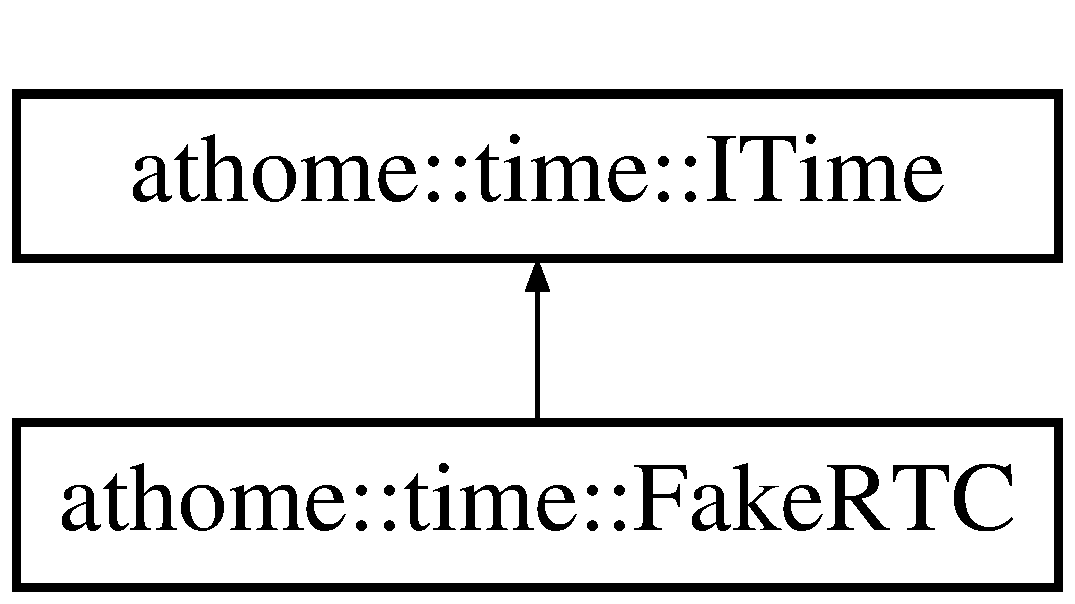
\includegraphics[height=2.000000cm]{classathome_1_1time_1_1_fake_r_t_c}
\end{center}
\end{figure}
\subsection*{Public Member Functions}
\begin{DoxyCompactItemize}
\item 
\mbox{\Hypertarget{classathome_1_1time_1_1_fake_r_t_c_a43e43ca95a5bbe16723030e1b67bd1ff}\label{classathome_1_1time_1_1_fake_r_t_c_a43e43ca95a5bbe16723030e1b67bd1ff}} 
{\bfseries Fake\+R\+TC} (const \mbox{\hyperlink{classathome_1_1time_1_1_fake_r_t_c}{Fake\+R\+TC}} \&)=delete
\item 
\mbox{\Hypertarget{classathome_1_1time_1_1_fake_r_t_c_ac7add5dcf5c8ef8112fc53c2e9a32778}\label{classathome_1_1time_1_1_fake_r_t_c_ac7add5dcf5c8ef8112fc53c2e9a32778}} 
\mbox{\hyperlink{classathome_1_1time_1_1_fake_r_t_c}{Fake\+R\+TC}} \& {\bfseries operator=} (const \mbox{\hyperlink{classathome_1_1time_1_1_fake_r_t_c}{Fake\+R\+TC}} \&)=delete
\item 
\mbox{\Hypertarget{classathome_1_1time_1_1_fake_r_t_c_a1559ff8bd889bdf02a40d3501864c6db}\label{classathome_1_1time_1_1_fake_r_t_c_a1559ff8bd889bdf02a40d3501864c6db}} 
virtual const I\+S\+O8601\+Date\+Time \& {\bfseries get\+Date\+Time} ()
\item 
\mbox{\Hypertarget{classathome_1_1time_1_1_fake_r_t_c_ab8565c9e7b300bf431cd0d636ad225b7}\label{classathome_1_1time_1_1_fake_r_t_c_ab8565c9e7b300bf431cd0d636ad225b7}} 
virtual void {\bfseries set\+Current\+Date\+Time} (const \mbox{\hyperlink{classathome_1_1time_1_1_i_time_1_1_date_time}{Date\+Time}} \&)
\end{DoxyCompactItemize}


The documentation for this class was generated from the following files\+:\begin{DoxyCompactItemize}
\item 
src/Fake\+R\+T\+C.\+hpp\item 
src/time/Fake\+R\+T\+C.\+cpp\end{DoxyCompactItemize}

\hypertarget{classathome_1_1display_1_1_grove_chainable_l_e_d}{}\section{athome\+:\+:display\+:\+:Grove\+Chainable\+L\+ED Class Reference}
\label{classathome_1_1display_1_1_grove_chainable_l_e_d}\index{athome\+::display\+::\+Grove\+Chainable\+L\+ED@{athome\+::display\+::\+Grove\+Chainable\+L\+ED}}
Inheritance diagram for athome\+:\+:display\+:\+:Grove\+Chainable\+L\+ED\+:\begin{figure}[H]
\begin{center}
\leavevmode
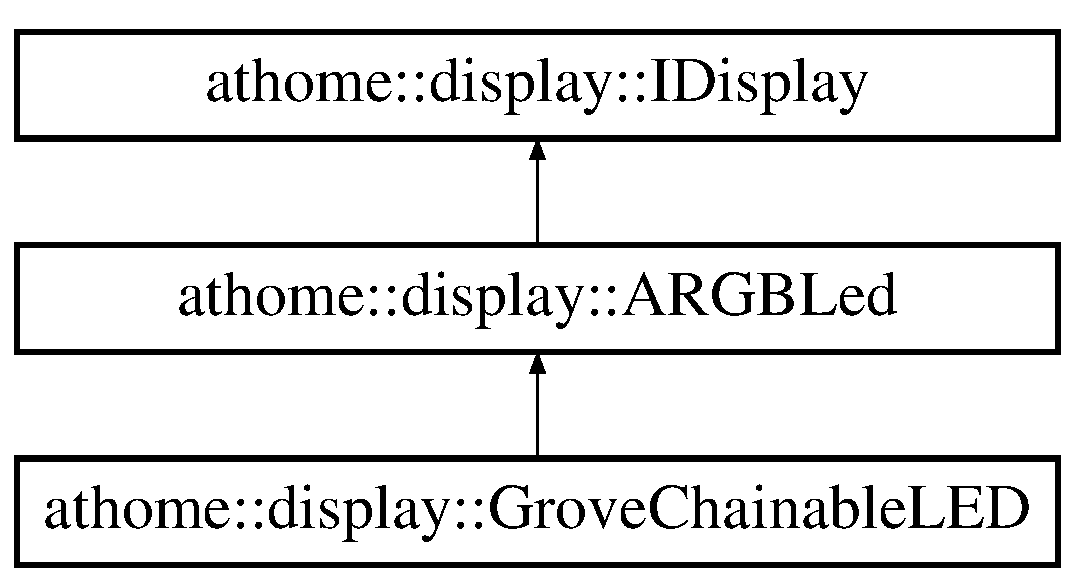
\includegraphics[height=3.000000cm]{classathome_1_1display_1_1_grove_chainable_l_e_d}
\end{center}
\end{figure}
\subsection*{Classes}
\begin{DoxyCompactItemize}
\item 
struct \mbox{\hyperlink{structathome_1_1display_1_1_grove_chainable_l_e_d_1_1_pins}{Pins}}
\end{DoxyCompactItemize}
\subsection*{Public Member Functions}
\begin{DoxyCompactItemize}
\item 
\mbox{\Hypertarget{classathome_1_1display_1_1_grove_chainable_l_e_d_af1ac9461a4d15ec2b9c18fbaab669ad4}\label{classathome_1_1display_1_1_grove_chainable_l_e_d_af1ac9461a4d15ec2b9c18fbaab669ad4}} 
{\bfseries Grove\+Chainable\+L\+ED} (const \mbox{\hyperlink{structathome_1_1display_1_1_grove_chainable_l_e_d_1_1_pins}{Pins}} $\ast$=nullptr)
\item 
\mbox{\Hypertarget{classathome_1_1display_1_1_grove_chainable_l_e_d_abe0361700f530eef79a1d9156de42da7}\label{classathome_1_1display_1_1_grove_chainable_l_e_d_abe0361700f530eef79a1d9156de42da7}} 
{\bfseries Grove\+Chainable\+L\+ED} (const \mbox{\hyperlink{structathome_1_1display_1_1_a_r_g_b_led_1_1_color}{A\+R\+G\+B\+Led\+::\+Color}} \&, const \mbox{\hyperlink{structathome_1_1display_1_1_grove_chainable_l_e_d_1_1_pins}{Pins}} $\ast$=nullptr)
\item 
\mbox{\Hypertarget{classathome_1_1display_1_1_grove_chainable_l_e_d_ae686988d0387af5bfe5f826219579f67}\label{classathome_1_1display_1_1_grove_chainable_l_e_d_ae686988d0387af5bfe5f826219579f67}} 
{\bfseries Grove\+Chainable\+L\+ED} (const \mbox{\hyperlink{classathome_1_1display_1_1_a_r_g_b_led}{A\+R\+G\+B\+Led}} \&, const \mbox{\hyperlink{structathome_1_1display_1_1_grove_chainable_l_e_d_1_1_pins}{Pins}} $\ast$=nullptr)
\item 
\mbox{\Hypertarget{classathome_1_1display_1_1_grove_chainable_l_e_d_a893e087b123d35cef059b8aaa4ddba28}\label{classathome_1_1display_1_1_grove_chainable_l_e_d_a893e087b123d35cef059b8aaa4ddba28}} 
\mbox{\hyperlink{classathome_1_1display_1_1_grove_chainable_l_e_d}{Grove\+Chainable\+L\+ED}} \& {\bfseries operator=} (const \mbox{\hyperlink{classathome_1_1display_1_1_a_r_g_b_led}{A\+R\+G\+B\+Led}} \&)
\item 
\mbox{\Hypertarget{classathome_1_1display_1_1_grove_chainable_l_e_d_a51ed72988d4313ab87e6ad492fc0c65a}\label{classathome_1_1display_1_1_grove_chainable_l_e_d_a51ed72988d4313ab87e6ad492fc0c65a}} 
\mbox{\hyperlink{classathome_1_1display_1_1_grove_chainable_l_e_d}{Grove\+Chainable\+L\+ED}} \& {\bfseries operator=} (const \mbox{\hyperlink{structathome_1_1display_1_1_a_r_g_b_led_1_1_color}{A\+R\+G\+B\+Led\+::\+Color}} \&)
\item 
virtual void \mbox{\hyperlink{classathome_1_1display_1_1_grove_chainable_l_e_d_a05a4a1381396b7fc11a24993865d8226}{update}} ()
\end{DoxyCompactItemize}
\subsection*{Protected Attributes}
\begin{DoxyCompactItemize}
\item 
\mbox{\Hypertarget{classathome_1_1display_1_1_grove_chainable_l_e_d_a4376da3d5ad9f1763aa6b3b45ec7e01a}\label{classathome_1_1display_1_1_grove_chainable_l_e_d_a4376da3d5ad9f1763aa6b3b45ec7e01a}} 
Chainable\+L\+ED $\ast$ {\bfseries \+\_\+led}
\end{DoxyCompactItemize}


\subsection{Member Function Documentation}
\mbox{\Hypertarget{classathome_1_1display_1_1_grove_chainable_l_e_d_a05a4a1381396b7fc11a24993865d8226}\label{classathome_1_1display_1_1_grove_chainable_l_e_d_a05a4a1381396b7fc11a24993865d8226}} 
\index{athome\+::display\+::\+Grove\+Chainable\+L\+ED@{athome\+::display\+::\+Grove\+Chainable\+L\+ED}!update@{update}}
\index{update@{update}!athome\+::display\+::\+Grove\+Chainable\+L\+ED@{athome\+::display\+::\+Grove\+Chainable\+L\+ED}}
\subsubsection{\texorpdfstring{update()}{update()}}
{\footnotesize\ttfamily void athome\+::display\+::\+Grove\+Chainable\+L\+E\+D\+::update (\begin{DoxyParamCaption}{ }\end{DoxyParamCaption})\hspace{0.3cm}{\ttfamily [virtual]}}

Update display content 

Implements \mbox{\hyperlink{classathome_1_1display_1_1_a_r_g_b_led_a725ceca0c01735daa9c95148baf075ab}{athome\+::display\+::\+A\+R\+G\+B\+Led}}.



The documentation for this class was generated from the following files\+:\begin{DoxyCompactItemize}
\item 
Grove\+Chainable\+L\+E\+D.\+hpp\item 
Grove\+Chainable\+L\+E\+D.\+cpp\end{DoxyCompactItemize}

\hypertarget{classathome_1_1display_1_1_i_display}{}\section{athome\+:\+:display\+:\+:I\+Display Class Reference}
\label{classathome_1_1display_1_1_i_display}\index{athome\+::display\+::\+I\+Display@{athome\+::display\+::\+I\+Display}}


{\ttfamily \#include $<$I\+Display.\+hpp$>$}

Inheritance diagram for athome\+:\+:display\+:\+:I\+Display\+:\begin{figure}[H]
\begin{center}
\leavevmode
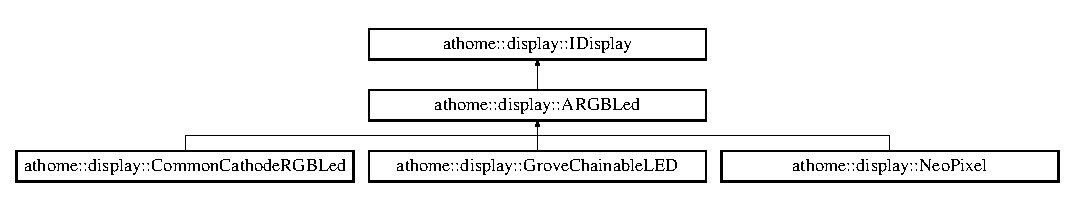
\includegraphics[height=1.660079cm]{classathome_1_1display_1_1_i_display}
\end{center}
\end{figure}
\subsection*{Public Member Functions}
\begin{DoxyCompactItemize}
\item 
virtual void \mbox{\hyperlink{classathome_1_1display_1_1_i_display_a0d3add1ce61c96657827fb56d250d9c6}{clear}} ()=0
\item 
virtual void \mbox{\hyperlink{classathome_1_1display_1_1_i_display_a4ba7bd5d46f88578f1c846f4f5f3c5d1}{update}} ()=0
\end{DoxyCompactItemize}


\subsection{Detailed Description}
Interface used to control any kind of display.

As the content displayed can change from on display to another (text, color, pixels, ...etc),

it has a very few common methods.

Unfortunately, embedded platforms tends to not have runtime (no {\ttfamily dynamic\+\_\+cast} or {\ttfamily typeof}), so user will have to manage the use of derived interfaces / classes by himself 

\subsection{Member Function Documentation}
\mbox{\Hypertarget{classathome_1_1display_1_1_i_display_a0d3add1ce61c96657827fb56d250d9c6}\label{classathome_1_1display_1_1_i_display_a0d3add1ce61c96657827fb56d250d9c6}} 
\index{athome\+::display\+::\+I\+Display@{athome\+::display\+::\+I\+Display}!clear@{clear}}
\index{clear@{clear}!athome\+::display\+::\+I\+Display@{athome\+::display\+::\+I\+Display}}
\subsubsection{\texorpdfstring{clear()}{clear()}}
{\footnotesize\ttfamily virtual void athome\+::display\+::\+I\+Display\+::clear (\begin{DoxyParamCaption}{ }\end{DoxyParamCaption})\hspace{0.3cm}{\ttfamily [pure virtual]}}

Remove display content 

Implemented in \mbox{\hyperlink{classathome_1_1display_1_1_a_r_g_b_led_a9753e3a23ea5cb6b0a41079bc6128766}{athome\+::display\+::\+A\+R\+G\+B\+Led}}.

\mbox{\Hypertarget{classathome_1_1display_1_1_i_display_a4ba7bd5d46f88578f1c846f4f5f3c5d1}\label{classathome_1_1display_1_1_i_display_a4ba7bd5d46f88578f1c846f4f5f3c5d1}} 
\index{athome\+::display\+::\+I\+Display@{athome\+::display\+::\+I\+Display}!update@{update}}
\index{update@{update}!athome\+::display\+::\+I\+Display@{athome\+::display\+::\+I\+Display}}
\subsubsection{\texorpdfstring{update()}{update()}}
{\footnotesize\ttfamily virtual void athome\+::display\+::\+I\+Display\+::update (\begin{DoxyParamCaption}{ }\end{DoxyParamCaption})\hspace{0.3cm}{\ttfamily [pure virtual]}}

Update display content 

Implemented in \mbox{\hyperlink{classathome_1_1display_1_1_a_r_g_b_led_a725ceca0c01735daa9c95148baf075ab}{athome\+::display\+::\+A\+R\+G\+B\+Led}}, \mbox{\hyperlink{classathome_1_1display_1_1_grove_chainable_l_e_d_a05a4a1381396b7fc11a24993865d8226}{athome\+::display\+::\+Grove\+Chainable\+L\+ED}}, \mbox{\hyperlink{classathome_1_1display_1_1_neo_pixel_a272bca4da78dff7dc02bcd023665e013}{athome\+::display\+::\+Neo\+Pixel}}, \mbox{\hyperlink{classathome_1_1display_1_1_common_anode_r_g_b_led_ab7daf7dcc6ac1e3fcab202cae484b237}{athome\+::display\+::\+Common\+Anode\+R\+G\+B\+Led}}, and \mbox{\hyperlink{classathome_1_1display_1_1_common_cathode_r_g_b_led_ab78ab6aef619d8e0941dd11d4cfbb545}{athome\+::display\+::\+Common\+Cathode\+R\+G\+B\+Led}}.



The documentation for this class was generated from the following file\+:\begin{DoxyCompactItemize}
\item 
I\+Display.\+hpp\end{DoxyCompactItemize}

\hypertarget{classathome_1_1power_1_1_i_power}{}\section{athome\+:\+:power\+:\+:I\+Power Class Reference}
\label{classathome_1_1power_1_1_i_power}\index{athome\+::power\+::\+I\+Power@{athome\+::power\+::\+I\+Power}}
\subsection*{Classes}
\begin{DoxyCompactItemize}
\item 
struct \mbox{\hyperlink{structathome_1_1power_1_1_i_power_1_1_power_info}{Power\+Info}}
\end{DoxyCompactItemize}
\subsection*{Public Types}
\begin{DoxyCompactItemize}
\item 
\mbox{\Hypertarget{classathome_1_1power_1_1_i_power_a0d23b118e64d97d708f2c6d153310107}\label{classathome_1_1power_1_1_i_power_a0d23b118e64d97d708f2c6d153310107}} 
enum {\bfseries S\+L\+E\+E\+P\+\_\+\+M\+O\+DE} \{ {\bfseries A\+C\+T\+I\+VE} = 0, 
{\bfseries L\+I\+G\+H\+T\+\_\+\+S\+L\+E\+EP}, 
{\bfseries S\+L\+E\+EP}, 
{\bfseries D\+E\+E\+P\+\_\+\+S\+L\+E\+EP}
 \}
\end{DoxyCompactItemize}
\subsection*{Public Member Functions}
\begin{DoxyCompactItemize}
\item 
\mbox{\Hypertarget{classathome_1_1power_1_1_i_power_a2b5a55274b0ad8619d9283a80063a4df}\label{classathome_1_1power_1_1_i_power_a2b5a55274b0ad8619d9283a80063a4df}} 
virtual const \mbox{\hyperlink{structathome_1_1power_1_1_i_power_1_1_power_info}{Power\+Info}} $\ast$ {\bfseries get\+Power\+Info} ()=0
\item 
\mbox{\Hypertarget{classathome_1_1power_1_1_i_power_ab6ff871c84bf451acbf11fa524193e2c}\label{classathome_1_1power_1_1_i_power_ab6ff871c84bf451acbf11fa524193e2c}} 
virtual void {\bfseries sleep} (S\+L\+E\+E\+P\+\_\+\+M\+O\+DE, uint32\+\_\+t)=0
\end{DoxyCompactItemize}


The documentation for this class was generated from the following file\+:\begin{DoxyCompactItemize}
\item 
src/I\+Power.\+hpp\end{DoxyCompactItemize}

\hypertarget{classathome_1_1sensor_1_1_i_sensor}{}\section{athome\+:\+:sensor\+:\+:I\+Sensor Class Reference}
\label{classathome_1_1sensor_1_1_i_sensor}\index{athome\+::sensor\+::\+I\+Sensor@{athome\+::sensor\+::\+I\+Sensor}}


{\ttfamily \#include $<$I\+Sensor.\+hpp$>$}

Inheritance diagram for athome\+:\+:sensor\+:\+:I\+Sensor\+:\begin{figure}[H]
\begin{center}
\leavevmode
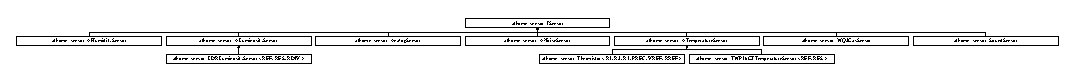
\includegraphics[height=0.629921cm]{classathome_1_1sensor_1_1_i_sensor}
\end{center}
\end{figure}
\subsection*{Classes}
\begin{DoxyCompactItemize}
\item 
struct \mbox{\hyperlink{structathome_1_1sensor_1_1_i_sensor_1_1_i_sensor_thresholds}{I\+Sensor\+Thresholds}}
\item 
struct \mbox{\hyperlink{structathome_1_1sensor_1_1_i_sensor_1_1_i_sensor_value}{I\+Sensor\+Value}}
\end{DoxyCompactItemize}
\subsection*{Public Types}
\begin{DoxyCompactItemize}
\item 
enum \mbox{\hyperlink{classathome_1_1sensor_1_1_i_sensor_aa70bc27a4c17c86caf96cca776541ddf}{I\+Sensor\+Scale}} \{ \newline
{\bfseries Z\+E\+RO}, 
{\bfseries O\+NE}, 
{\bfseries T\+WO}, 
{\bfseries T\+H\+R\+EE}, 
\newline
{\bfseries F\+O\+UR}, 
{\bfseries F\+I\+VE}, 
{\bfseries S\+IX}, 
{\bfseries S\+E\+V\+EN}, 
\newline
{\bfseries E\+I\+G\+HT}, 
{\bfseries N\+I\+NE}, 
{\bfseries T\+EN}
 \}
\end{DoxyCompactItemize}
\subsection*{Public Member Functions}
\begin{DoxyCompactItemize}
\item 
virtual const \mbox{\hyperlink{structathome_1_1sensor_1_1_i_sensor_1_1_i_sensor_value}{I\+Sensor\+Value}} \& \mbox{\hyperlink{classathome_1_1sensor_1_1_i_sensor_ae109cd3741ea9c88dc7e4f2eaf1485d5}{get\+Sample}} ()=0
\item 
virtual void \mbox{\hyperlink{classathome_1_1sensor_1_1_i_sensor_af86df8538fecfcfc670b4adfbbde6abb}{set\+Thresholds}} (const \mbox{\hyperlink{structathome_1_1sensor_1_1_i_sensor_1_1_i_sensor_thresholds}{I\+Sensor\+Thresholds}} \&)=0
\end{DoxyCompactItemize}


\subsection{Detailed Description}
Interface used to grab data from a sensor in a Module class.

Configuration and treatment of sensor raw data is to be handled by derived classes, as this interfaces is intended to be able to just being able to grab raw sensors data, and an interpretation of them without any knowledge of the sensor. 

\subsection{Member Enumeration Documentation}
\mbox{\Hypertarget{classathome_1_1sensor_1_1_i_sensor_aa70bc27a4c17c86caf96cca776541ddf}\label{classathome_1_1sensor_1_1_i_sensor_aa70bc27a4c17c86caf96cca776541ddf}} 
\index{athome\+::sensor\+::\+I\+Sensor@{athome\+::sensor\+::\+I\+Sensor}!I\+Sensor\+Scale@{I\+Sensor\+Scale}}
\index{I\+Sensor\+Scale@{I\+Sensor\+Scale}!athome\+::sensor\+::\+I\+Sensor@{athome\+::sensor\+::\+I\+Sensor}}
\subsubsection{\texorpdfstring{I\+Sensor\+Scale}{ISensorScale}}
{\footnotesize\ttfamily enum \mbox{\hyperlink{classathome_1_1sensor_1_1_i_sensor_aa70bc27a4c17c86caf96cca776541ddf}{athome\+::sensor\+::\+I\+Sensor\+::\+I\+Sensor\+Scale}}}

Enumeration used to represent the estimation of safety of a sensor value on a scale from 1 to 10. Value 0 means invalid 

\subsection{Member Function Documentation}
\mbox{\Hypertarget{classathome_1_1sensor_1_1_i_sensor_ae109cd3741ea9c88dc7e4f2eaf1485d5}\label{classathome_1_1sensor_1_1_i_sensor_ae109cd3741ea9c88dc7e4f2eaf1485d5}} 
\index{athome\+::sensor\+::\+I\+Sensor@{athome\+::sensor\+::\+I\+Sensor}!get\+Sample@{get\+Sample}}
\index{get\+Sample@{get\+Sample}!athome\+::sensor\+::\+I\+Sensor@{athome\+::sensor\+::\+I\+Sensor}}
\subsubsection{\texorpdfstring{get\+Sample()}{getSample()}}
{\footnotesize\ttfamily virtual const \mbox{\hyperlink{structathome_1_1sensor_1_1_i_sensor_1_1_i_sensor_value}{I\+Sensor\+Value}}\& athome\+::sensor\+::\+I\+Sensor\+::get\+Sample (\begin{DoxyParamCaption}{ }\end{DoxyParamCaption})\hspace{0.3cm}{\ttfamily [pure virtual]}}

Returns a pointer on sensor sample raw memory, as an array of bytes 

Implemented in \mbox{\hyperlink{classathome_1_1sensor_1_1_m_q2_gas_sensor_adbe1195490ce67fbed7c717abe2b5b13}{athome\+::sensor\+::\+M\+Q2\+Gas\+Sensor}}, \mbox{\hyperlink{classathome_1_1sensor_1_1_analog_sensor_a7ad00f985a9d1abeb64f973b5d16558c}{athome\+::sensor\+::\+Analog\+Sensor}}, \mbox{\hyperlink{classathome_1_1sensor_1_1_a_luminosity_sensor_a6e0e7bcfe13cd8d8edf6a09f6e230ef8}{athome\+::sensor\+::\+A\+Luminosity\+Sensor}}, \mbox{\hyperlink{classathome_1_1sensor_1_1_sound_sensor_a8ac5f417eee873247aff8a7e96e12817}{athome\+::sensor\+::\+Sound\+Sensor}}, \mbox{\hyperlink{classathome_1_1sensor_1_1_a_temperature_sensor_afea6a461b8dff9ee736aa508aa4f6a3c}{athome\+::sensor\+::\+A\+Temperature\+Sensor}}, \mbox{\hyperlink{classathome_1_1sensor_1_1_a_humidity_sensor_a7af4527c70b539bec58cecfaae0aa80e}{athome\+::sensor\+::\+A\+Humidity\+Sensor}}, and \mbox{\hyperlink{classathome_1_1sensor_1_1_a_noise_sensor_ab567b050b41bd0b72fcc9b94b9f6fc6e}{athome\+::sensor\+::\+A\+Noise\+Sensor}}.

\mbox{\Hypertarget{classathome_1_1sensor_1_1_i_sensor_af86df8538fecfcfc670b4adfbbde6abb}\label{classathome_1_1sensor_1_1_i_sensor_af86df8538fecfcfc670b4adfbbde6abb}} 
\index{athome\+::sensor\+::\+I\+Sensor@{athome\+::sensor\+::\+I\+Sensor}!set\+Thresholds@{set\+Thresholds}}
\index{set\+Thresholds@{set\+Thresholds}!athome\+::sensor\+::\+I\+Sensor@{athome\+::sensor\+::\+I\+Sensor}}
\subsubsection{\texorpdfstring{set\+Thresholds()}{setThresholds()}}
{\footnotesize\ttfamily virtual void athome\+::sensor\+::\+I\+Sensor\+::set\+Thresholds (\begin{DoxyParamCaption}\item[{const \mbox{\hyperlink{structathome_1_1sensor_1_1_i_sensor_1_1_i_sensor_thresholds}{I\+Sensor\+Thresholds}} \&}]{ }\end{DoxyParamCaption})\hspace{0.3cm}{\ttfamily [pure virtual]}}

Returns the estimation of safety from the current sensor value

Example\+:


\begin{DoxyCode}
\textcolor{keywordtype}{void} my\_function\_telling\_if\_a\_sensor\_value\_is\_good\_or\_not(ISensor
&my\_sensor) \{ \mbox{\hyperlink{classathome_1_1sensor_1_1_i_sensor_aa70bc27a4c17c86caf96cca776541ddf}{ISensorScale}} sensor\_estimate = my\_sensor.getEstimate(); \textcolor{keywordflow}{if}
(sensor\_estimate == ISensor::ZERO) \{ Serial.println(\textcolor{stringliteral}{"The sensor returned an}
\textcolor{stringliteral}{invalid value"});
  \}
  \textcolor{keywordflow}{else} \textcolor{keywordflow}{if} (sensor\_estimate > ISensor::ZERO && sensor\_estimate < 6) \{
    Serial.println(\textcolor{stringliteral}{"Boouh, it's not good :("});
  \}
  \textcolor{keywordflow}{else} \{
    Serial.println(\textcolor{stringliteral}{"Yaaaay!"});
  \}
\}
\end{DoxyCode}
 

Implemented in \mbox{\hyperlink{classathome_1_1sensor_1_1_m_q2_gas_sensor_a69de9f45b9babd2d111b4ce020d7c83e}{athome\+::sensor\+::\+M\+Q2\+Gas\+Sensor}}, \mbox{\hyperlink{classathome_1_1sensor_1_1_analog_sensor_addcdb79aa03b7b6e386bc9c59faced10}{athome\+::sensor\+::\+Analog\+Sensor}}, \mbox{\hyperlink{classathome_1_1sensor_1_1_a_luminosity_sensor_aa26ed7176ba600f6900bd249edce71ab}{athome\+::sensor\+::\+A\+Luminosity\+Sensor}}, \mbox{\hyperlink{classathome_1_1sensor_1_1_sound_sensor_adaf42abe0443f486361656efe9587ba7}{athome\+::sensor\+::\+Sound\+Sensor}}, \mbox{\hyperlink{classathome_1_1sensor_1_1_a_temperature_sensor_a1c323184ac116784e877151895dfd080}{athome\+::sensor\+::\+A\+Temperature\+Sensor}}, \mbox{\hyperlink{classathome_1_1sensor_1_1_a_humidity_sensor_a1a19bfee3db6b0940f1329b42d7ed0d0}{athome\+::sensor\+::\+A\+Humidity\+Sensor}}, and \mbox{\hyperlink{classathome_1_1sensor_1_1_a_noise_sensor_a8429e91e9f8b2e1634a405780f456beb}{athome\+::sensor\+::\+A\+Noise\+Sensor}}.



The documentation for this class was generated from the following file\+:\begin{DoxyCompactItemize}
\item 
src/I\+Sensor.\+hpp\end{DoxyCompactItemize}

\hypertarget{structathome_1_1sensor_1_1_i_sensor_1_1_i_sensor_thresholds}{}\section{athome\+:\+:sensor\+:\+:I\+Sensor\+:\+:I\+Sensor\+Thresholds Struct Reference}
\label{structathome_1_1sensor_1_1_i_sensor_1_1_i_sensor_thresholds}\index{athome\+::sensor\+::\+I\+Sensor\+::\+I\+Sensor\+Thresholds@{athome\+::sensor\+::\+I\+Sensor\+::\+I\+Sensor\+Thresholds}}
\subsection*{Public Attributes}
\begin{DoxyCompactItemize}
\item 
\mbox{\Hypertarget{structathome_1_1sensor_1_1_i_sensor_1_1_i_sensor_thresholds_a14489c021cea49fd39052766083b3255}\label{structathome_1_1sensor_1_1_i_sensor_1_1_i_sensor_thresholds_a14489c021cea49fd39052766083b3255}} 
\mbox{\hyperlink{structathome_1_1utility_1_1units_1_1_unit}{utility\+::units\+::\+Unit}} {\bfseries unit}
\item 
\mbox{\Hypertarget{structathome_1_1sensor_1_1_i_sensor_1_1_i_sensor_thresholds_a2bed3181d271e07d6c6a51611e838362}\label{structathome_1_1sensor_1_1_i_sensor_1_1_i_sensor_thresholds_a2bed3181d271e07d6c6a51611e838362}} 
uint32\+\_\+t {\bfseries min}
\item 
\mbox{\Hypertarget{structathome_1_1sensor_1_1_i_sensor_1_1_i_sensor_thresholds_af8911a22468fed64c40fee4451bcca8a}\label{structathome_1_1sensor_1_1_i_sensor_1_1_i_sensor_thresholds_af8911a22468fed64c40fee4451bcca8a}} 
uint32\+\_\+t {\bfseries max}
\end{DoxyCompactItemize}


The documentation for this struct was generated from the following file\+:\begin{DoxyCompactItemize}
\item 
src/I\+Sensor.\+hpp\end{DoxyCompactItemize}

\hypertarget{structathome_1_1sensor_1_1_i_sensor_1_1_i_sensor_value}{}\section{athome\+:\+:sensor\+:\+:I\+Sensor\+:\+:I\+Sensor\+Value Struct Reference}
\label{structathome_1_1sensor_1_1_i_sensor_1_1_i_sensor_value}\index{athome\+::sensor\+::\+I\+Sensor\+::\+I\+Sensor\+Value@{athome\+::sensor\+::\+I\+Sensor\+::\+I\+Sensor\+Value}}
\subsection*{Public Attributes}
\begin{DoxyCompactItemize}
\item 
\mbox{\Hypertarget{structathome_1_1sensor_1_1_i_sensor_1_1_i_sensor_value_a3f5ef42b7996bf59549e80fd95dcaa87}\label{structathome_1_1sensor_1_1_i_sensor_1_1_i_sensor_value_a3f5ef42b7996bf59549e80fd95dcaa87}} 
\mbox{\hyperlink{classathome_1_1sensor_1_1_i_sensor_aa70bc27a4c17c86caf96cca776541ddf}{I\+Sensor\+Scale}} {\bfseries estimate}
\item 
\mbox{\Hypertarget{structathome_1_1sensor_1_1_i_sensor_1_1_i_sensor_value_a35ceaf0b4f9e3586a154b33b00e8e83d}\label{structathome_1_1sensor_1_1_i_sensor_1_1_i_sensor_value_a35ceaf0b4f9e3586a154b33b00e8e83d}} 
\mbox{\hyperlink{structathome_1_1utility_1_1units_1_1_unit}{utility\+::units\+::\+Unit}} {\bfseries unit}
\item 
\mbox{\Hypertarget{structathome_1_1sensor_1_1_i_sensor_1_1_i_sensor_value_a3afa32e47ab7c385a51f55bcb6597ae7}\label{structathome_1_1sensor_1_1_i_sensor_1_1_i_sensor_value_a3afa32e47ab7c385a51f55bcb6597ae7}} 
void $\ast$ {\bfseries sample\+Raw\+Pointer}
\item 
\mbox{\Hypertarget{structathome_1_1sensor_1_1_i_sensor_1_1_i_sensor_value_a8eeef7fadc2c6b97ff8d1279f655d038}\label{structathome_1_1sensor_1_1_i_sensor_1_1_i_sensor_value_a8eeef7fadc2c6b97ff8d1279f655d038}} 
P\+G\+M\+\_\+P {\bfseries label}
\end{DoxyCompactItemize}


The documentation for this struct was generated from the following file\+:\begin{DoxyCompactItemize}
\item 
src/I\+Sensor.\+hpp\end{DoxyCompactItemize}

\hypertarget{structathome_1_1time_1_1_i_time_1_1_i_s_o8601_date_time}{}\section{athome\+:\+:time\+:\+:I\+Time\+:\+:I\+S\+O8601\+Date\+Time Struct Reference}
\label{structathome_1_1time_1_1_i_time_1_1_i_s_o8601_date_time}\index{athome\+::time\+::\+I\+Time\+::\+I\+S\+O8601\+Date\+Time@{athome\+::time\+::\+I\+Time\+::\+I\+S\+O8601\+Date\+Time}}
Inheritance diagram for athome\+:\+:time\+:\+:I\+Time\+:\+:I\+S\+O8601\+Date\+Time\+:\begin{figure}[H]
\begin{center}
\leavevmode
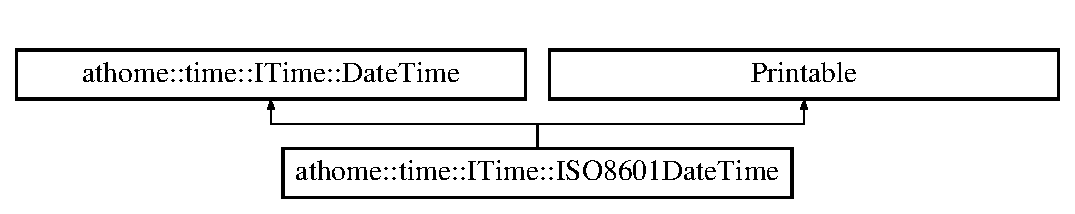
\includegraphics[height=2.000000cm]{structathome_1_1time_1_1_i_time_1_1_i_s_o8601_date_time}
\end{center}
\end{figure}
\subsection*{Public Member Functions}
\begin{DoxyCompactItemize}
\item 
\mbox{\Hypertarget{structathome_1_1time_1_1_i_time_1_1_i_s_o8601_date_time_a61bde2502a373b8305b5bde4cf7df075}\label{structathome_1_1time_1_1_i_time_1_1_i_s_o8601_date_time_a61bde2502a373b8305b5bde4cf7df075}} 
virtual size\+\_\+t {\bfseries print\+To} (Print \&p) const
\item 
\mbox{\Hypertarget{structathome_1_1time_1_1_i_time_1_1_i_s_o8601_date_time_a66eca189bb7e28995c7ee6922991018b}\label{structathome_1_1time_1_1_i_time_1_1_i_s_o8601_date_time_a66eca189bb7e28995c7ee6922991018b}} 
\mbox{\hyperlink{structathome_1_1time_1_1_i_time_1_1_i_s_o8601_date_time}{I\+S\+O8601\+Date\+Time}} \& {\bfseries operator=} (const \mbox{\hyperlink{classathome_1_1time_1_1_i_time_1_1_date_time}{Date\+Time}} \&date)
\end{DoxyCompactItemize}
\subsection*{Additional Inherited Members}


The documentation for this struct was generated from the following file\+:\begin{DoxyCompactItemize}
\item 
src/I\+Time.\+hpp\end{DoxyCompactItemize}

\hypertarget{classathome_1_1storage_1_1_i_storage}{}\section{athome\+:\+:storage\+:\+:I\+Storage Class Reference}
\label{classathome_1_1storage_1_1_i_storage}\index{athome\+::storage\+::\+I\+Storage@{athome\+::storage\+::\+I\+Storage}}


{\ttfamily \#include $<$I\+Storage.\+hpp$>$}

Inheritance diagram for athome\+:\+:storage\+:\+:I\+Storage\+:\begin{figure}[H]
\begin{center}
\leavevmode
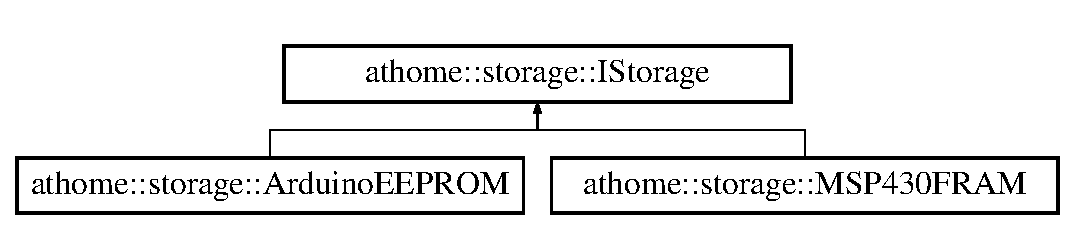
\includegraphics[height=2.000000cm]{classathome_1_1storage_1_1_i_storage}
\end{center}
\end{figure}
\subsection*{Public Member Functions}
\begin{DoxyCompactItemize}
\item 
virtual void \mbox{\hyperlink{classathome_1_1storage_1_1_i_storage_af623393cdf559addf167463ce4e7005e}{read}} (size\+\_\+t, void $\ast$, size\+\_\+t)=0
\item 
virtual void \mbox{\hyperlink{classathome_1_1storage_1_1_i_storage_a1017bb6ad438313b98197893954e52f1}{write}} (size\+\_\+t, const void $\ast$, size\+\_\+t)=0
\end{DoxyCompactItemize}


\subsection{Detailed Description}
Interface used to be able to store and read raw data from any source, by transferring memory buffers 

\subsection{Member Function Documentation}
\mbox{\Hypertarget{classathome_1_1storage_1_1_i_storage_af623393cdf559addf167463ce4e7005e}\label{classathome_1_1storage_1_1_i_storage_af623393cdf559addf167463ce4e7005e}} 
\index{athome\+::storage\+::\+I\+Storage@{athome\+::storage\+::\+I\+Storage}!read@{read}}
\index{read@{read}!athome\+::storage\+::\+I\+Storage@{athome\+::storage\+::\+I\+Storage}}
\subsubsection{\texorpdfstring{read()}{read()}}
{\footnotesize\ttfamily virtual void athome\+::storage\+::\+I\+Storage\+::read (\begin{DoxyParamCaption}\item[{size\+\_\+t}]{,  }\item[{void $\ast$}]{,  }\item[{size\+\_\+t}]{ }\end{DoxyParamCaption})\hspace{0.3cm}{\ttfamily [pure virtual]}}

Copy n bytes (3rd parameter) in dest (2nd parameter) from offset x (1st parameter)

Example\+:


\begin{DoxyCode}
\textcolor{keywordtype}{void} my\_function\_reading\_something(IStorage &storage) \{
  \textcolor{keywordtype}{char} my\_string[33];
  \textcolor{keywordtype}{int} my\_number;

  storage.read(0, my\_string, \textcolor{keyword}{sizeof}(my\_string)); \textcolor{comment}{// Reading a string (array}
of 33 char) at offset 0 of storage instance into my\_string
  storage.read(\textcolor{keyword}{sizeof}(my\_string), &my\_number, \textcolor{keyword}{sizeof}(my\_number)); \textcolor{comment}{//}
Reading an integer at offset 33 (after content put into my\_string) from
storage instance into my\_number
\}
\end{DoxyCode}
 

Implemented in \mbox{\hyperlink{classathome_1_1storage_1_1_m_s_p430_f_r_a_m_a3a00a26565491d08d26f505930453fb7}{athome\+::storage\+::\+M\+S\+P430\+F\+R\+AM}}, and \mbox{\hyperlink{classathome_1_1storage_1_1_arduino_e_e_p_r_o_m_a853674189981dd3395ea76911d2eb1a0}{athome\+::storage\+::\+Arduino\+E\+E\+P\+R\+OM}}.

\mbox{\Hypertarget{classathome_1_1storage_1_1_i_storage_a1017bb6ad438313b98197893954e52f1}\label{classathome_1_1storage_1_1_i_storage_a1017bb6ad438313b98197893954e52f1}} 
\index{athome\+::storage\+::\+I\+Storage@{athome\+::storage\+::\+I\+Storage}!write@{write}}
\index{write@{write}!athome\+::storage\+::\+I\+Storage@{athome\+::storage\+::\+I\+Storage}}
\subsubsection{\texorpdfstring{write()}{write()}}
{\footnotesize\ttfamily virtual void athome\+::storage\+::\+I\+Storage\+::write (\begin{DoxyParamCaption}\item[{size\+\_\+t}]{,  }\item[{const void $\ast$}]{,  }\item[{size\+\_\+t}]{ }\end{DoxyParamCaption})\hspace{0.3cm}{\ttfamily [pure virtual]}}

Write n bytes (3rd parameter) in offset x (1st parameter) from src (2nd parameter)

Example\+:


\begin{DoxyCode}
\textcolor{keywordtype}{void} my\_function\_writing\_something(IStorage &storage) \{
  \textcolor{keywordtype}{char} my\_string[] = \textcolor{stringliteral}{"Hello, World!"};
  \textcolor{keywordtype}{int} my\_number = 42;

  storage.write(0, my\_string, \textcolor{keyword}{sizeof}(my\_string)); \textcolor{comment}{// Writing the string}
(array of 14 char) my\_string at offset 0 of storage instance
  storage.write(\textcolor{keyword}{sizeof}(my\_string), &my\_number, \textcolor{keyword}{sizeof}(my\_number)); \textcolor{comment}{//}
Writing my\_number at offset 14 (after my\_string) of storage instance
\}
\end{DoxyCode}
 

Implemented in \mbox{\hyperlink{classathome_1_1storage_1_1_m_s_p430_f_r_a_m_ae6b7a6d178233f9e54394360b34c3bca}{athome\+::storage\+::\+M\+S\+P430\+F\+R\+AM}}, and \mbox{\hyperlink{classathome_1_1storage_1_1_arduino_e_e_p_r_o_m_a20027ab8a5b20c1fad3e3e42daafe53d}{athome\+::storage\+::\+Arduino\+E\+E\+P\+R\+OM}}.



The documentation for this class was generated from the following file\+:\begin{DoxyCompactItemize}
\item 
src/I\+Storage.\+hpp\end{DoxyCompactItemize}

\hypertarget{structathome_1_1time_1_1_i_time}{}\section{athome\+:\+:time\+:\+:I\+Time Struct Reference}
\label{structathome_1_1time_1_1_i_time}\index{athome\+::time\+::\+I\+Time@{athome\+::time\+::\+I\+Time}}
Inheritance diagram for athome\+:\+:time\+:\+:I\+Time\+:\begin{figure}[H]
\begin{center}
\leavevmode
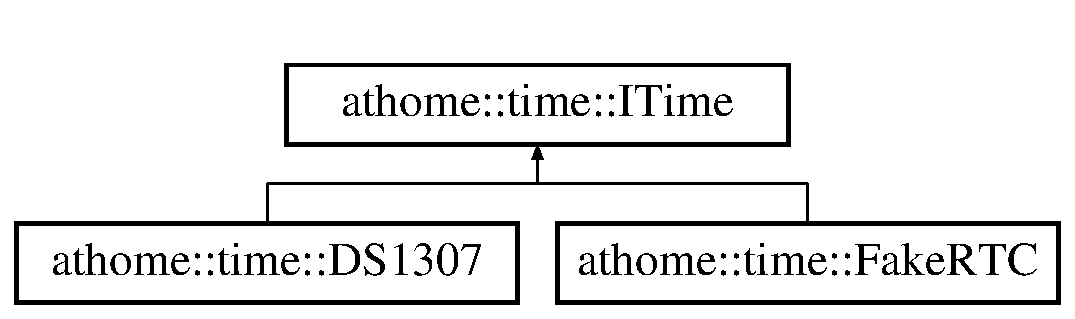
\includegraphics[height=2.000000cm]{structathome_1_1time_1_1_i_time}
\end{center}
\end{figure}
\subsection*{Classes}
\begin{DoxyCompactItemize}
\item 
struct \mbox{\hyperlink{structathome_1_1time_1_1_i_time_1_1_date_time}{Date\+Time}}
\end{DoxyCompactItemize}
\subsection*{Public Member Functions}
\begin{DoxyCompactItemize}
\item 
\mbox{\Hypertarget{structathome_1_1time_1_1_i_time_a5ffc0cb263c36f1c466fe29322925db7}\label{structathome_1_1time_1_1_i_time_a5ffc0cb263c36f1c466fe29322925db7}} 
virtual const \mbox{\hyperlink{structathome_1_1time_1_1_i_time_1_1_date_time}{Date\+Time}} \& {\bfseries get\+Date\+Time} ()=0
\item 
\mbox{\Hypertarget{structathome_1_1time_1_1_i_time_acfcb9e53a8202ade38ab38d2639ebb7b}\label{structathome_1_1time_1_1_i_time_acfcb9e53a8202ade38ab38d2639ebb7b}} 
virtual void {\bfseries set\+Current\+Date\+Time} (const \mbox{\hyperlink{structathome_1_1time_1_1_i_time_1_1_date_time}{Date\+Time}} \&)=0
\end{DoxyCompactItemize}


The documentation for this struct was generated from the following file\+:\begin{DoxyCompactItemize}
\item 
src/I\+Time.\+hpp\end{DoxyCompactItemize}

\hypertarget{classathome_1_1sensor_1_1_l_d_r_luminosity_sensor}{}\section{athome\+:\+:sensor\+:\+:L\+D\+R\+Luminosity\+Sensor$<$ R\+EF, R\+ES, R\+D\+IV $>$ Class Template Reference}
\label{classathome_1_1sensor_1_1_l_d_r_luminosity_sensor}\index{athome\+::sensor\+::\+L\+D\+R\+Luminosity\+Sensor$<$ R\+E\+F, R\+E\+S, R\+D\+I\+V $>$@{athome\+::sensor\+::\+L\+D\+R\+Luminosity\+Sensor$<$ R\+E\+F, R\+E\+S, R\+D\+I\+V $>$}}
Inheritance diagram for athome\+:\+:sensor\+:\+:L\+D\+R\+Luminosity\+Sensor$<$ R\+EF, R\+ES, R\+D\+IV $>$\+:\begin{figure}[H]
\begin{center}
\leavevmode
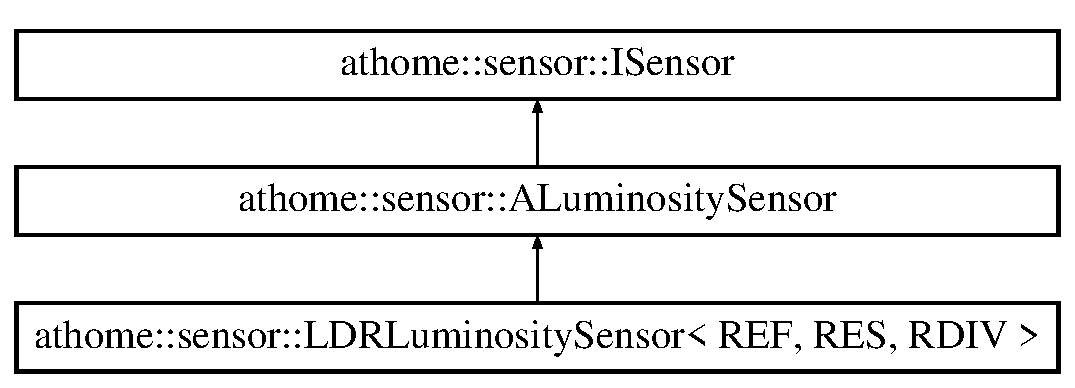
\includegraphics[height=3.000000cm]{classathome_1_1sensor_1_1_l_d_r_luminosity_sensor}
\end{center}
\end{figure}
\subsection*{Public Member Functions}
\begin{DoxyCompactItemize}
\item 
\mbox{\Hypertarget{classathome_1_1sensor_1_1_l_d_r_luminosity_sensor_aee1ab68d020e97e6ec526a4b11e6f4fc}\label{classathome_1_1sensor_1_1_l_d_r_luminosity_sensor_aee1ab68d020e97e6ec526a4b11e6f4fc}} 
{\bfseries L\+D\+R\+Luminosity\+Sensor} (uint8\+\_\+t pin)
\item 
\mbox{\Hypertarget{classathome_1_1sensor_1_1_l_d_r_luminosity_sensor_a7a3c5ffb280c13acdcd5444963f7a32f}\label{classathome_1_1sensor_1_1_l_d_r_luminosity_sensor_a7a3c5ffb280c13acdcd5444963f7a32f}} 
{\bfseries L\+D\+R\+Luminosity\+Sensor} (const \mbox{\hyperlink{classathome_1_1sensor_1_1_l_d_r_luminosity_sensor}{L\+D\+R\+Luminosity\+Sensor}} \&)=delete
\item 
\mbox{\Hypertarget{classathome_1_1sensor_1_1_l_d_r_luminosity_sensor_ab9e7d3d92fb16c7464d7a2f6c39a42fa}\label{classathome_1_1sensor_1_1_l_d_r_luminosity_sensor_ab9e7d3d92fb16c7464d7a2f6c39a42fa}} 
\mbox{\hyperlink{classathome_1_1sensor_1_1_l_d_r_luminosity_sensor}{L\+D\+R\+Luminosity\+Sensor}} \& {\bfseries operator=} (const \mbox{\hyperlink{classathome_1_1sensor_1_1_l_d_r_luminosity_sensor}{L\+D\+R\+Luminosity\+Sensor}} \&)=delete
\item 
uint16\+\_\+t \mbox{\hyperlink{classathome_1_1sensor_1_1_l_d_r_luminosity_sensor_a6e4f25000704564ce30a7e3531f23c43}{get\+Sensor\+Sample}} ()
\end{DoxyCompactItemize}
\subsection*{Additional Inherited Members}


\subsection{Member Function Documentation}
\mbox{\Hypertarget{classathome_1_1sensor_1_1_l_d_r_luminosity_sensor_a6e4f25000704564ce30a7e3531f23c43}\label{classathome_1_1sensor_1_1_l_d_r_luminosity_sensor_a6e4f25000704564ce30a7e3531f23c43}} 
\index{athome\+::sensor\+::\+L\+D\+R\+Luminosity\+Sensor@{athome\+::sensor\+::\+L\+D\+R\+Luminosity\+Sensor}!get\+Sensor\+Sample@{get\+Sensor\+Sample}}
\index{get\+Sensor\+Sample@{get\+Sensor\+Sample}!athome\+::sensor\+::\+L\+D\+R\+Luminosity\+Sensor@{athome\+::sensor\+::\+L\+D\+R\+Luminosity\+Sensor}}
\subsubsection{\texorpdfstring{get\+Sensor\+Sample()}{getSensorSample()}}
{\footnotesize\ttfamily template$<$uint32\+\_\+t R\+EF, uint32\+\_\+t R\+ES, uint32\+\_\+t R\+D\+IV$>$ \\
uint16\+\_\+t \mbox{\hyperlink{classathome_1_1sensor_1_1_l_d_r_luminosity_sensor}{athome\+::sensor\+::\+L\+D\+R\+Luminosity\+Sensor}}$<$ R\+EF, R\+ES, R\+D\+IV $>$\+::get\+Sensor\+Sample (\begin{DoxyParamCaption}{ }\end{DoxyParamCaption})\hspace{0.3cm}{\ttfamily [inline]}, {\ttfamily [virtual]}}

Return the number of lux as an integer. 

Implements \mbox{\hyperlink{classathome_1_1sensor_1_1_a_luminosity_sensor_ae756f7d7647c2cf695305c8f11aec8d3}{athome\+::sensor\+::\+A\+Luminosity\+Sensor}}.



The documentation for this class was generated from the following file\+:\begin{DoxyCompactItemize}
\item 
src/L\+D\+R\+Luminosity\+Sensor.\+hpp\end{DoxyCompactItemize}

\hypertarget{classathome_1_1display_1_1_monochromatic_l_e_d}{}\section{athome\+:\+:display\+:\+:Monochromatic\+L\+ED Class Reference}
\label{classathome_1_1display_1_1_monochromatic_l_e_d}\index{athome\+::display\+::\+Monochromatic\+L\+ED@{athome\+::display\+::\+Monochromatic\+L\+ED}}
Inheritance diagram for athome\+:\+:display\+:\+:Monochromatic\+L\+ED\+:\begin{figure}[H]
\begin{center}
\leavevmode
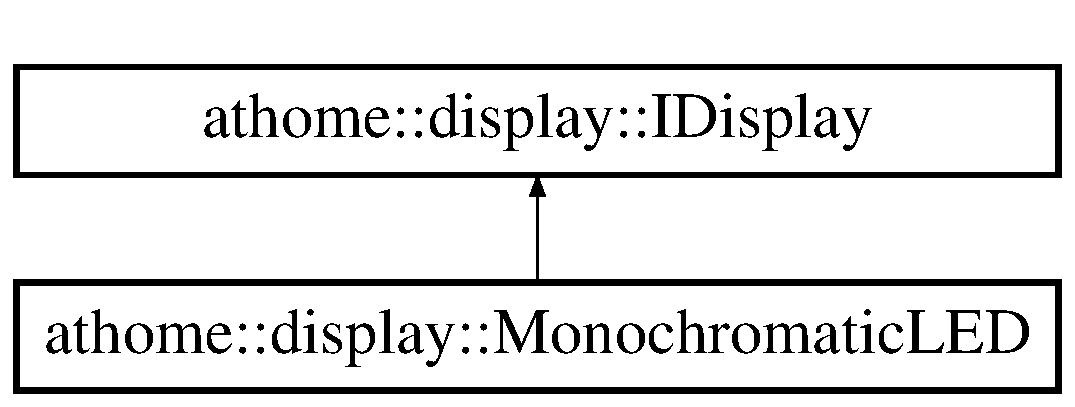
\includegraphics[height=2.000000cm]{classathome_1_1display_1_1_monochromatic_l_e_d}
\end{center}
\end{figure}
\subsection*{Public Member Functions}
\begin{DoxyCompactItemize}
\item 
\mbox{\Hypertarget{classathome_1_1display_1_1_monochromatic_l_e_d_a39e97eaa9f1cbad0288db45f4c94d834}\label{classathome_1_1display_1_1_monochromatic_l_e_d_a39e97eaa9f1cbad0288db45f4c94d834}} 
{\bfseries Monochromatic\+L\+ED} (int, bool=false)
\item 
\mbox{\Hypertarget{classathome_1_1display_1_1_monochromatic_l_e_d_aaafb0861e538c07e1b55d622cda8859a}\label{classathome_1_1display_1_1_monochromatic_l_e_d_aaafb0861e538c07e1b55d622cda8859a}} 
{\bfseries Monochromatic\+L\+ED} (const \mbox{\hyperlink{classathome_1_1display_1_1_monochromatic_l_e_d}{Monochromatic\+L\+ED}} \&)=delete
\item 
\mbox{\Hypertarget{classathome_1_1display_1_1_monochromatic_l_e_d_a9b204c11983e469ed8c111689a5d318e}\label{classathome_1_1display_1_1_monochromatic_l_e_d_a9b204c11983e469ed8c111689a5d318e}} 
\mbox{\hyperlink{classathome_1_1display_1_1_monochromatic_l_e_d}{Monochromatic\+L\+ED}} \& {\bfseries operator=} (const \mbox{\hyperlink{classathome_1_1display_1_1_monochromatic_l_e_d}{Monochromatic\+L\+ED}} \&)=delete
\item 
virtual void \mbox{\hyperlink{classathome_1_1display_1_1_monochromatic_l_e_d_a81a1470c33e639e916f014e5adbe8707}{clear}} ()
\item 
virtual void \mbox{\hyperlink{classathome_1_1display_1_1_monochromatic_l_e_d_aef6a651fdbb24ebb1d0887c1b3e5133d}{update}} ()
\item 
virtual void \mbox{\hyperlink{classathome_1_1display_1_1_monochromatic_l_e_d_a67a39b7d73305a98fc25705dcc5f3cd0}{set\+Displayed\+Estimate}} (\mbox{\hyperlink{classathome_1_1sensor_1_1_i_sensor_aa70bc27a4c17c86caf96cca776541ddf}{sensor\+::\+I\+Sensor\+::\+I\+Sensor\+Scale}})
\end{DoxyCompactItemize}


\subsection{Member Function Documentation}
\mbox{\Hypertarget{classathome_1_1display_1_1_monochromatic_l_e_d_a81a1470c33e639e916f014e5adbe8707}\label{classathome_1_1display_1_1_monochromatic_l_e_d_a81a1470c33e639e916f014e5adbe8707}} 
\index{athome\+::display\+::\+Monochromatic\+L\+ED@{athome\+::display\+::\+Monochromatic\+L\+ED}!clear@{clear}}
\index{clear@{clear}!athome\+::display\+::\+Monochromatic\+L\+ED@{athome\+::display\+::\+Monochromatic\+L\+ED}}
\subsubsection{\texorpdfstring{clear()}{clear()}}
{\footnotesize\ttfamily void athome\+::display\+::\+Monochromatic\+L\+E\+D\+::clear (\begin{DoxyParamCaption}{ }\end{DoxyParamCaption})\hspace{0.3cm}{\ttfamily [virtual]}}

Remove display content 

Implements \mbox{\hyperlink{classathome_1_1display_1_1_i_display_a0d3add1ce61c96657827fb56d250d9c6}{athome\+::display\+::\+I\+Display}}.

\mbox{\Hypertarget{classathome_1_1display_1_1_monochromatic_l_e_d_a67a39b7d73305a98fc25705dcc5f3cd0}\label{classathome_1_1display_1_1_monochromatic_l_e_d_a67a39b7d73305a98fc25705dcc5f3cd0}} 
\index{athome\+::display\+::\+Monochromatic\+L\+ED@{athome\+::display\+::\+Monochromatic\+L\+ED}!set\+Displayed\+Estimate@{set\+Displayed\+Estimate}}
\index{set\+Displayed\+Estimate@{set\+Displayed\+Estimate}!athome\+::display\+::\+Monochromatic\+L\+ED@{athome\+::display\+::\+Monochromatic\+L\+ED}}
\subsubsection{\texorpdfstring{set\+Displayed\+Estimate()}{setDisplayedEstimate()}}
{\footnotesize\ttfamily void athome\+::display\+::\+Monochromatic\+L\+E\+D\+::set\+Displayed\+Estimate (\begin{DoxyParamCaption}\item[{\mbox{\hyperlink{classathome_1_1sensor_1_1_i_sensor_aa70bc27a4c17c86caf96cca776541ddf}{sensor\+::\+I\+Sensor\+::\+I\+Sensor\+Scale}}}]{ }\end{DoxyParamCaption})\hspace{0.3cm}{\ttfamily [virtual]}}

Set the value displayed on the screen, whatever the type of display is.

I\+Sensor\+Scale is an enumeration representing the correctness on a scale from 1 to 10 (1 is worst, 10 is best).

This scale can be represented by various ways for many different displays. For example\+:


\begin{DoxyItemize}
\item An L\+ED could stay off from 6 and on below 6
\item A dimmable L\+ED could set it\textquotesingle{}s percentage of brightness corresponding to the value (for example 1 = 100\%, 5 = 50\%, 10 = 0\%)
\item A 7 segments display could display the digit itself and stay off at 10
\item An L\+CD screen could write a sentence, the digit, draw a gauge, ...etc
\item A speaker or buzzer could do noise of different intensities below 6
\item ...etc 
\end{DoxyItemize}

Implements \mbox{\hyperlink{classathome_1_1display_1_1_i_display_a3c9678f929e4bc04742d458b0c2399ef}{athome\+::display\+::\+I\+Display}}.

\mbox{\Hypertarget{classathome_1_1display_1_1_monochromatic_l_e_d_aef6a651fdbb24ebb1d0887c1b3e5133d}\label{classathome_1_1display_1_1_monochromatic_l_e_d_aef6a651fdbb24ebb1d0887c1b3e5133d}} 
\index{athome\+::display\+::\+Monochromatic\+L\+ED@{athome\+::display\+::\+Monochromatic\+L\+ED}!update@{update}}
\index{update@{update}!athome\+::display\+::\+Monochromatic\+L\+ED@{athome\+::display\+::\+Monochromatic\+L\+ED}}
\subsubsection{\texorpdfstring{update()}{update()}}
{\footnotesize\ttfamily void athome\+::display\+::\+Monochromatic\+L\+E\+D\+::update (\begin{DoxyParamCaption}{ }\end{DoxyParamCaption})\hspace{0.3cm}{\ttfamily [virtual]}}

Update display content 

Implements \mbox{\hyperlink{classathome_1_1display_1_1_i_display_a4ba7bd5d46f88578f1c846f4f5f3c5d1}{athome\+::display\+::\+I\+Display}}.



The documentation for this class was generated from the following files\+:\begin{DoxyCompactItemize}
\item 
src/Monochromatic\+L\+E\+D.\+hpp\item 
src/display/Monochromatic\+L\+E\+D.\+cpp\end{DoxyCompactItemize}

\hypertarget{classathome_1_1sensor_1_1_m_q2_gas_sensor}{}\section{athome\+:\+:sensor\+:\+:M\+Q2\+Gas\+Sensor Class Reference}
\label{classathome_1_1sensor_1_1_m_q2_gas_sensor}\index{athome\+::sensor\+::\+M\+Q2\+Gas\+Sensor@{athome\+::sensor\+::\+M\+Q2\+Gas\+Sensor}}
Inheritance diagram for athome\+:\+:sensor\+:\+:M\+Q2\+Gas\+Sensor\+:\begin{figure}[H]
\begin{center}
\leavevmode
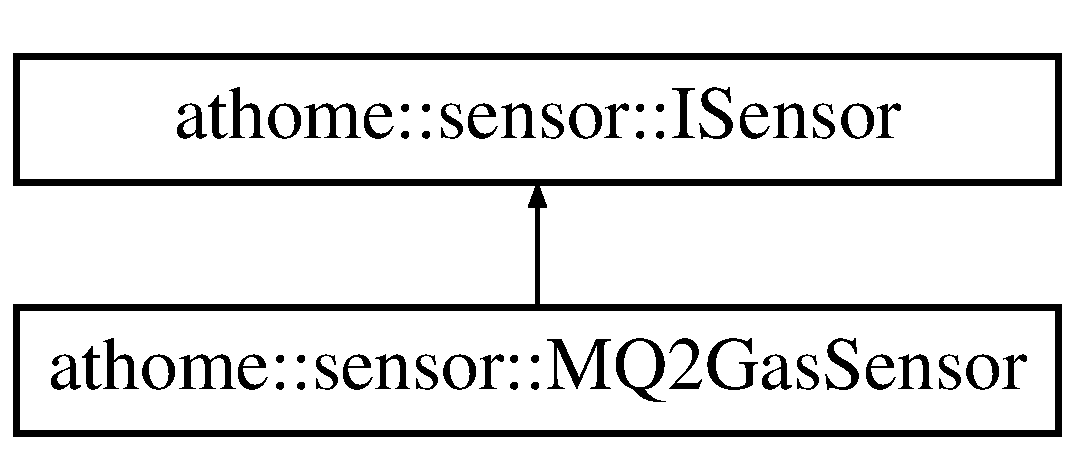
\includegraphics[height=2.000000cm]{classathome_1_1sensor_1_1_m_q2_gas_sensor}
\end{center}
\end{figure}
\subsection*{Classes}
\begin{DoxyCompactItemize}
\item 
struct \mbox{\hyperlink{structathome_1_1sensor_1_1_m_q2_gas_sensor_1_1_values}{Values}}
\end{DoxyCompactItemize}
\subsection*{Public Member Functions}
\begin{DoxyCompactItemize}
\item 
\mbox{\Hypertarget{classathome_1_1sensor_1_1_m_q2_gas_sensor_aa311f792931e425c6d9d77bded775dfa}\label{classathome_1_1sensor_1_1_m_q2_gas_sensor_aa311f792931e425c6d9d77bded775dfa}} 
{\bfseries M\+Q2\+Gas\+Sensor} (int pin)
\item 
\mbox{\Hypertarget{classathome_1_1sensor_1_1_m_q2_gas_sensor_a93bc43d684f3d225bf5baab8048752b8}\label{classathome_1_1sensor_1_1_m_q2_gas_sensor_a93bc43d684f3d225bf5baab8048752b8}} 
{\bfseries M\+Q2\+Gas\+Sensor} (const \mbox{\hyperlink{classathome_1_1sensor_1_1_m_q2_gas_sensor}{M\+Q2\+Gas\+Sensor}} \&)=delete
\item 
\mbox{\Hypertarget{classathome_1_1sensor_1_1_m_q2_gas_sensor_ab57873a8ee1bdf20619d6efa090bdd40}\label{classathome_1_1sensor_1_1_m_q2_gas_sensor_ab57873a8ee1bdf20619d6efa090bdd40}} 
\mbox{\hyperlink{classathome_1_1sensor_1_1_m_q2_gas_sensor}{M\+Q2\+Gas\+Sensor}} \& {\bfseries operator=} (const \mbox{\hyperlink{classathome_1_1sensor_1_1_m_q2_gas_sensor}{M\+Q2\+Gas\+Sensor}} \&)=delete
\item 
int \mbox{\hyperlink{classathome_1_1sensor_1_1_m_q2_gas_sensor_a6bf60231a95fe2ba2f5bc9c1bad714c5}{M\+Q\+Get\+Percentage}} (float rs\+\_\+ro\+\_\+ratio, float $\ast$pcurve)
\item 
\mbox{\Hypertarget{classathome_1_1sensor_1_1_m_q2_gas_sensor_a872737bb858eb7e6310fb5675d0b3b72}\label{classathome_1_1sensor_1_1_m_q2_gas_sensor_a872737bb858eb7e6310fb5675d0b3b72}} 
void {\bfseries set\+Pin} (int pin)
\item 
\mbox{\Hypertarget{classathome_1_1sensor_1_1_m_q2_gas_sensor_a70221cb17fc88bb3784e00da53d67975}\label{classathome_1_1sensor_1_1_m_q2_gas_sensor_a70221cb17fc88bb3784e00da53d67975}} 
int {\bfseries get\+Pin} () const
\item 
int \mbox{\hyperlink{classathome_1_1sensor_1_1_m_q2_gas_sensor_a65401612b298d829987c2b75ead8f246}{get\+L\+PG}} () const
\item 
int \mbox{\hyperlink{classathome_1_1sensor_1_1_m_q2_gas_sensor_aa6e3ad7d0382f04cf15388fd36722579}{get\+Smoke}} () const
\item 
int \mbox{\hyperlink{classathome_1_1sensor_1_1_m_q2_gas_sensor_a36cce0ec962d8b5269e39ee4c368be67}{get\+CO}} () const
\item 
const \mbox{\hyperlink{structathome_1_1sensor_1_1_i_sensor_1_1_i_sensor_value}{I\+Sensor\+Value}} \& \mbox{\hyperlink{classathome_1_1sensor_1_1_m_q2_gas_sensor_adbe1195490ce67fbed7c717abe2b5b13}{get\+Sample}} ()
\item 
void \mbox{\hyperlink{classathome_1_1sensor_1_1_m_q2_gas_sensor_a69de9f45b9babd2d111b4ce020d7c83e}{set\+Thresholds}} (const \mbox{\hyperlink{structathome_1_1sensor_1_1_i_sensor_1_1_i_sensor_thresholds}{I\+Sensor\+Thresholds}} \&)
\end{DoxyCompactItemize}
\subsection*{Additional Inherited Members}


\subsection{Member Function Documentation}
\mbox{\Hypertarget{classathome_1_1sensor_1_1_m_q2_gas_sensor_a36cce0ec962d8b5269e39ee4c368be67}\label{classathome_1_1sensor_1_1_m_q2_gas_sensor_a36cce0ec962d8b5269e39ee4c368be67}} 
\index{athome\+::sensor\+::\+M\+Q2\+Gas\+Sensor@{athome\+::sensor\+::\+M\+Q2\+Gas\+Sensor}!get\+CO@{get\+CO}}
\index{get\+CO@{get\+CO}!athome\+::sensor\+::\+M\+Q2\+Gas\+Sensor@{athome\+::sensor\+::\+M\+Q2\+Gas\+Sensor}}
\subsubsection{\texorpdfstring{get\+C\+O()}{getCO()}}
{\footnotesize\ttfamily int athome\+::sensor\+::\+M\+Q2\+Gas\+Sensor\+::get\+CO (\begin{DoxyParamCaption}{ }\end{DoxyParamCaption}) const}

Only Possible when get\+Value is called /!\textbackslash{}

\begin{DoxyReturn}{Returns}
value of CO contain in a struct (struct.\+co) 
\end{DoxyReturn}
\mbox{\Hypertarget{classathome_1_1sensor_1_1_m_q2_gas_sensor_a65401612b298d829987c2b75ead8f246}\label{classathome_1_1sensor_1_1_m_q2_gas_sensor_a65401612b298d829987c2b75ead8f246}} 
\index{athome\+::sensor\+::\+M\+Q2\+Gas\+Sensor@{athome\+::sensor\+::\+M\+Q2\+Gas\+Sensor}!get\+L\+PG@{get\+L\+PG}}
\index{get\+L\+PG@{get\+L\+PG}!athome\+::sensor\+::\+M\+Q2\+Gas\+Sensor@{athome\+::sensor\+::\+M\+Q2\+Gas\+Sensor}}
\subsubsection{\texorpdfstring{get\+L\+P\+G()}{getLPG()}}
{\footnotesize\ttfamily int athome\+::sensor\+::\+M\+Q2\+Gas\+Sensor\+::get\+L\+PG (\begin{DoxyParamCaption}{ }\end{DoxyParamCaption}) const}

Only Possible when get\+Value is called /!\textbackslash{}

\begin{DoxyReturn}{Returns}
value of L\+PG contain in a struct (struct.\+lpg) 
\end{DoxyReturn}
\mbox{\Hypertarget{classathome_1_1sensor_1_1_m_q2_gas_sensor_adbe1195490ce67fbed7c717abe2b5b13}\label{classathome_1_1sensor_1_1_m_q2_gas_sensor_adbe1195490ce67fbed7c717abe2b5b13}} 
\index{athome\+::sensor\+::\+M\+Q2\+Gas\+Sensor@{athome\+::sensor\+::\+M\+Q2\+Gas\+Sensor}!get\+Sample@{get\+Sample}}
\index{get\+Sample@{get\+Sample}!athome\+::sensor\+::\+M\+Q2\+Gas\+Sensor@{athome\+::sensor\+::\+M\+Q2\+Gas\+Sensor}}
\subsubsection{\texorpdfstring{get\+Sample()}{getSample()}}
{\footnotesize\ttfamily const \mbox{\hyperlink{structathome_1_1sensor_1_1_i_sensor_1_1_i_sensor_value}{I\+Sensor\+::\+I\+Sensor\+Value}} \& athome\+::sensor\+::\+M\+Q2\+Gas\+Sensor\+::get\+Sample (\begin{DoxyParamCaption}{ }\end{DoxyParamCaption})\hspace{0.3cm}{\ttfamily [virtual]}}

Returns a pointer on sensor sample raw memory, as an array of bytes 

Implements \mbox{\hyperlink{classathome_1_1sensor_1_1_i_sensor_ae109cd3741ea9c88dc7e4f2eaf1485d5}{athome\+::sensor\+::\+I\+Sensor}}.

\mbox{\Hypertarget{classathome_1_1sensor_1_1_m_q2_gas_sensor_aa6e3ad7d0382f04cf15388fd36722579}\label{classathome_1_1sensor_1_1_m_q2_gas_sensor_aa6e3ad7d0382f04cf15388fd36722579}} 
\index{athome\+::sensor\+::\+M\+Q2\+Gas\+Sensor@{athome\+::sensor\+::\+M\+Q2\+Gas\+Sensor}!get\+Smoke@{get\+Smoke}}
\index{get\+Smoke@{get\+Smoke}!athome\+::sensor\+::\+M\+Q2\+Gas\+Sensor@{athome\+::sensor\+::\+M\+Q2\+Gas\+Sensor}}
\subsubsection{\texorpdfstring{get\+Smoke()}{getSmoke()}}
{\footnotesize\ttfamily int athome\+::sensor\+::\+M\+Q2\+Gas\+Sensor\+::get\+Smoke (\begin{DoxyParamCaption}{ }\end{DoxyParamCaption}) const}

Only Possible when get\+Value is called /!\textbackslash{}

\begin{DoxyReturn}{Returns}
value of S\+M\+O\+KE contain in a struct (struct.\+smoke) 
\end{DoxyReturn}
\mbox{\Hypertarget{classathome_1_1sensor_1_1_m_q2_gas_sensor_a6bf60231a95fe2ba2f5bc9c1bad714c5}\label{classathome_1_1sensor_1_1_m_q2_gas_sensor_a6bf60231a95fe2ba2f5bc9c1bad714c5}} 
\index{athome\+::sensor\+::\+M\+Q2\+Gas\+Sensor@{athome\+::sensor\+::\+M\+Q2\+Gas\+Sensor}!M\+Q\+Get\+Percentage@{M\+Q\+Get\+Percentage}}
\index{M\+Q\+Get\+Percentage@{M\+Q\+Get\+Percentage}!athome\+::sensor\+::\+M\+Q2\+Gas\+Sensor@{athome\+::sensor\+::\+M\+Q2\+Gas\+Sensor}}
\subsubsection{\texorpdfstring{M\+Q\+Get\+Percentage()}{MQGetPercentage()}}
{\footnotesize\ttfamily int athome\+::sensor\+::\+M\+Q2\+Gas\+Sensor\+::\+M\+Q\+Get\+Percentage (\begin{DoxyParamCaption}\item[{float}]{rs\+\_\+ro\+\_\+ratio,  }\item[{float $\ast$}]{pcurve }\end{DoxyParamCaption})}

Input\+: rs\+\_\+ro\+\_\+ratio\+: Rs divided by Ro pcurve

pointer to the curve of the target gas

Output\+: ppm of the target gas

Remarks\+: By using the slope and a point of the line. The x(logarithmic value of ppm) of the line could be derived if y(rs\+\_\+ro\+\_\+ratio) is provided. As it is a logarithmic coordinate, power of 10 is used to convert the result to non-\/logarithmic value. \mbox{\Hypertarget{classathome_1_1sensor_1_1_m_q2_gas_sensor_a69de9f45b9babd2d111b4ce020d7c83e}\label{classathome_1_1sensor_1_1_m_q2_gas_sensor_a69de9f45b9babd2d111b4ce020d7c83e}} 
\index{athome\+::sensor\+::\+M\+Q2\+Gas\+Sensor@{athome\+::sensor\+::\+M\+Q2\+Gas\+Sensor}!set\+Thresholds@{set\+Thresholds}}
\index{set\+Thresholds@{set\+Thresholds}!athome\+::sensor\+::\+M\+Q2\+Gas\+Sensor@{athome\+::sensor\+::\+M\+Q2\+Gas\+Sensor}}
\subsubsection{\texorpdfstring{set\+Thresholds()}{setThresholds()}}
{\footnotesize\ttfamily void athome\+::sensor\+::\+M\+Q2\+Gas\+Sensor\+::set\+Thresholds (\begin{DoxyParamCaption}\item[{const \mbox{\hyperlink{structathome_1_1sensor_1_1_i_sensor_1_1_i_sensor_thresholds}{I\+Sensor\+Thresholds}} \&}]{ }\end{DoxyParamCaption})\hspace{0.3cm}{\ttfamily [virtual]}}

Returns the estimation of safety from the current sensor value

Example\+:


\begin{DoxyCode}
\textcolor{keywordtype}{void} my\_function\_telling\_if\_a\_sensor\_value\_is\_good\_or\_not(ISensor
&my\_sensor) \{ \mbox{\hyperlink{classathome_1_1sensor_1_1_i_sensor_aa70bc27a4c17c86caf96cca776541ddf}{ISensorScale}} sensor\_estimate = my\_sensor.getEstimate(); \textcolor{keywordflow}{if}
(sensor\_estimate == ISensor::ZERO) \{ Serial.println(\textcolor{stringliteral}{"The sensor returned an}
\textcolor{stringliteral}{invalid value"});
  \}
  \textcolor{keywordflow}{else} \textcolor{keywordflow}{if} (sensor\_estimate > ISensor::ZERO && sensor\_estimate < 6) \{
    Serial.println(\textcolor{stringliteral}{"Boouh, it's not good :("});
  \}
  \textcolor{keywordflow}{else} \{
    Serial.println(\textcolor{stringliteral}{"Yaaaay!"});
  \}
\}
\end{DoxyCode}
 

Implements \mbox{\hyperlink{classathome_1_1sensor_1_1_i_sensor_af86df8538fecfcfc670b4adfbbde6abb}{athome\+::sensor\+::\+I\+Sensor}}.



The documentation for this class was generated from the following files\+:\begin{DoxyCompactItemize}
\item 
src/M\+Q2\+Gas\+Sensor.\+hpp\item 
src/sensor/air\+\_\+quality/M\+Q2\+Gas\+Sensor.\+cpp\end{DoxyCompactItemize}

\hypertarget{classathome_1_1storage_1_1_m_s_p430_f_r_a_m}{}\section{athome\+:\+:storage\+:\+:M\+S\+P430\+F\+R\+AM Class Reference}
\label{classathome_1_1storage_1_1_m_s_p430_f_r_a_m}\index{athome\+::storage\+::\+M\+S\+P430\+F\+R\+AM@{athome\+::storage\+::\+M\+S\+P430\+F\+R\+AM}}


{\ttfamily \#include $<$M\+S\+P430\+F\+R\+A\+M.\+hpp$>$}

Inheritance diagram for athome\+:\+:storage\+:\+:M\+S\+P430\+F\+R\+AM\+:\begin{figure}[H]
\begin{center}
\leavevmode
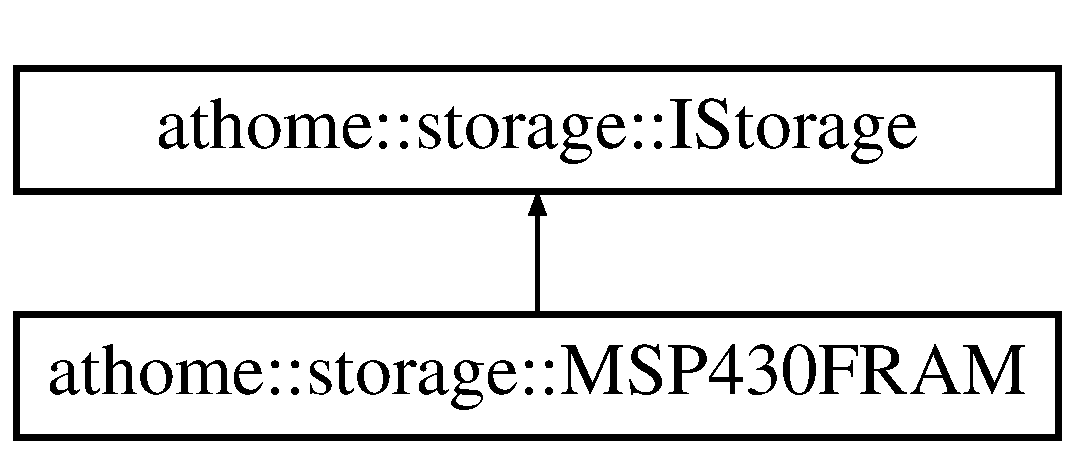
\includegraphics[height=2.000000cm]{classathome_1_1storage_1_1_m_s_p430_f_r_a_m}
\end{center}
\end{figure}
\subsection*{Public Member Functions}
\begin{DoxyCompactItemize}
\item 
\mbox{\Hypertarget{classathome_1_1storage_1_1_m_s_p430_f_r_a_m_a4537357b5eb4195cff71461bb8f97300}\label{classathome_1_1storage_1_1_m_s_p430_f_r_a_m_a4537357b5eb4195cff71461bb8f97300}} 
{\bfseries M\+S\+P430\+F\+R\+AM} (const \mbox{\hyperlink{classathome_1_1storage_1_1_m_s_p430_f_r_a_m}{M\+S\+P430\+F\+R\+AM}} \&)=delete
\item 
\mbox{\Hypertarget{classathome_1_1storage_1_1_m_s_p430_f_r_a_m_aa6bceeda133dc8e69af41ec1c86811c5}\label{classathome_1_1storage_1_1_m_s_p430_f_r_a_m_aa6bceeda133dc8e69af41ec1c86811c5}} 
\mbox{\hyperlink{classathome_1_1storage_1_1_m_s_p430_f_r_a_m}{M\+S\+P430\+F\+R\+AM}} \& {\bfseries operator=} (const \mbox{\hyperlink{classathome_1_1storage_1_1_m_s_p430_f_r_a_m}{M\+S\+P430\+F\+R\+AM}} \&)=delete
\item 
virtual void \mbox{\hyperlink{classathome_1_1storage_1_1_m_s_p430_f_r_a_m_a3a00a26565491d08d26f505930453fb7}{read}} (size\+\_\+t, void $\ast$, size\+\_\+t)
\item 
virtual void \mbox{\hyperlink{classathome_1_1storage_1_1_m_s_p430_f_r_a_m_ae6b7a6d178233f9e54394360b34c3bca}{write}} (size\+\_\+t, const void $\ast$, size\+\_\+t)
\end{DoxyCompactItemize}
\subsection*{Static Public Member Functions}
\begin{DoxyCompactItemize}
\item 
\mbox{\Hypertarget{classathome_1_1storage_1_1_m_s_p430_f_r_a_m_aafeeb8882c31af72dfa4054e27263fa6}\label{classathome_1_1storage_1_1_m_s_p430_f_r_a_m_aafeeb8882c31af72dfa4054e27263fa6}} 
static \mbox{\hyperlink{classathome_1_1storage_1_1_m_s_p430_f_r_a_m}{M\+S\+P430\+F\+R\+AM}} $\ast$ {\bfseries get\+Instance} ()
\end{DoxyCompactItemize}


\subsection{Detailed Description}
Singleton enabling to store persistent data in the F\+R\+AM of TI Launchpads.

The size of the persistent storage is defined by the macro A\+T\+H\+O\+M\+E\+\_\+\+F\+R\+A\+M\+\_\+\+S\+T\+O\+R\+A\+G\+E\+\_\+\+S\+I\+ZE and has a default value of 255 bytes.

This can be overriden by the user by defining this macro at the compilation, such as passing the {\ttfamily -\/\+D\+A\+T\+H\+O\+M\+E\+\_\+\+F\+R\+A\+M\+\_\+\+S\+T\+O\+R\+A\+G\+E\+\_\+\+S\+I\+ZE=} option with G\+CC 

\subsection{Member Function Documentation}
\mbox{\Hypertarget{classathome_1_1storage_1_1_m_s_p430_f_r_a_m_a3a00a26565491d08d26f505930453fb7}\label{classathome_1_1storage_1_1_m_s_p430_f_r_a_m_a3a00a26565491d08d26f505930453fb7}} 
\index{athome\+::storage\+::\+M\+S\+P430\+F\+R\+AM@{athome\+::storage\+::\+M\+S\+P430\+F\+R\+AM}!read@{read}}
\index{read@{read}!athome\+::storage\+::\+M\+S\+P430\+F\+R\+AM@{athome\+::storage\+::\+M\+S\+P430\+F\+R\+AM}}
\subsubsection{\texorpdfstring{read()}{read()}}
{\footnotesize\ttfamily void athome\+::storage\+::\+M\+S\+P430\+F\+R\+A\+M\+::read (\begin{DoxyParamCaption}\item[{size\+\_\+t}]{,  }\item[{void $\ast$}]{,  }\item[{size\+\_\+t}]{ }\end{DoxyParamCaption})\hspace{0.3cm}{\ttfamily [virtual]}}

Copy n bytes (3rd parameter) in dest (2nd parameter) from offset x (1st parameter)

Example\+:


\begin{DoxyCode}
\textcolor{keywordtype}{void} my\_function\_reading\_something(IStorage &storage) \{
  \textcolor{keywordtype}{char} my\_string[33];
  \textcolor{keywordtype}{int} my\_number;

  storage.read(0, my\_string, \textcolor{keyword}{sizeof}(my\_string)); \textcolor{comment}{// Reading a string (array of 33 char) at offset 0 of
       storage instance into my\_string}
  storage.read(\textcolor{keyword}{sizeof}(my\_string), &my\_number, \textcolor{keyword}{sizeof}(my\_number)); \textcolor{comment}{// Reading an integer at offset 33 (after
       content put into my\_string) from storage instance into my\_number}
\}
\end{DoxyCode}
 

Implements \mbox{\hyperlink{classathome_1_1storage_1_1_i_storage_af623393cdf559addf167463ce4e7005e}{athome\+::storage\+::\+I\+Storage}}.

\mbox{\Hypertarget{classathome_1_1storage_1_1_m_s_p430_f_r_a_m_ae6b7a6d178233f9e54394360b34c3bca}\label{classathome_1_1storage_1_1_m_s_p430_f_r_a_m_ae6b7a6d178233f9e54394360b34c3bca}} 
\index{athome\+::storage\+::\+M\+S\+P430\+F\+R\+AM@{athome\+::storage\+::\+M\+S\+P430\+F\+R\+AM}!write@{write}}
\index{write@{write}!athome\+::storage\+::\+M\+S\+P430\+F\+R\+AM@{athome\+::storage\+::\+M\+S\+P430\+F\+R\+AM}}
\subsubsection{\texorpdfstring{write()}{write()}}
{\footnotesize\ttfamily void athome\+::storage\+::\+M\+S\+P430\+F\+R\+A\+M\+::write (\begin{DoxyParamCaption}\item[{size\+\_\+t}]{,  }\item[{const void $\ast$}]{,  }\item[{size\+\_\+t}]{ }\end{DoxyParamCaption})\hspace{0.3cm}{\ttfamily [virtual]}}

Write n bytes (3rd parameter) in offset x (1st parameter) from src (2nd parameter)

Example\+:


\begin{DoxyCode}
\textcolor{keywordtype}{void} my\_function\_writing\_something(IStorage &storage) \{
  \textcolor{keywordtype}{char} my\_string[] = \textcolor{stringliteral}{"Hello, World!"};
  \textcolor{keywordtype}{int} my\_number = 42;

  storage.write(0, my\_string, \textcolor{keyword}{sizeof}(my\_string)); \textcolor{comment}{// Writing the string (array of 14 char) my\_string at
       offset 0 of storage instance}
  storage.write(\textcolor{keyword}{sizeof}(my\_string), &my\_number, \textcolor{keyword}{sizeof}(my\_number)); \textcolor{comment}{// Writing my\_number at offset 14 (after
       my\_string) of storage instance}
\}
\end{DoxyCode}
 

Implements \mbox{\hyperlink{classathome_1_1storage_1_1_i_storage_a1017bb6ad438313b98197893954e52f1}{athome\+::storage\+::\+I\+Storage}}.



The documentation for this class was generated from the following files\+:\begin{DoxyCompactItemize}
\item 
src/M\+S\+P430\+F\+R\+A\+M.\+hpp\item 
src/storage/M\+S\+P430\+F\+R\+A\+M.\+cpp\end{DoxyCompactItemize}

\hypertarget{classathome_1_1communication_1_1wifi_1_1_native_arduino_e_s_p_wi_fi_communicator}{}\section{athome\+:\+:communication\+:\+:wifi\+:\+:Native\+Arduino\+E\+S\+P\+Wi\+Fi\+Communicator Class Reference}
\label{classathome_1_1communication_1_1wifi_1_1_native_arduino_e_s_p_wi_fi_communicator}\index{athome\+::communication\+::wifi\+::\+Native\+Arduino\+E\+S\+P\+Wi\+Fi\+Communicator@{athome\+::communication\+::wifi\+::\+Native\+Arduino\+E\+S\+P\+Wi\+Fi\+Communicator}}
Inheritance diagram for athome\+:\+:communication\+:\+:wifi\+:\+:Native\+Arduino\+E\+S\+P\+Wi\+Fi\+Communicator\+:\begin{figure}[H]
\begin{center}
\leavevmode
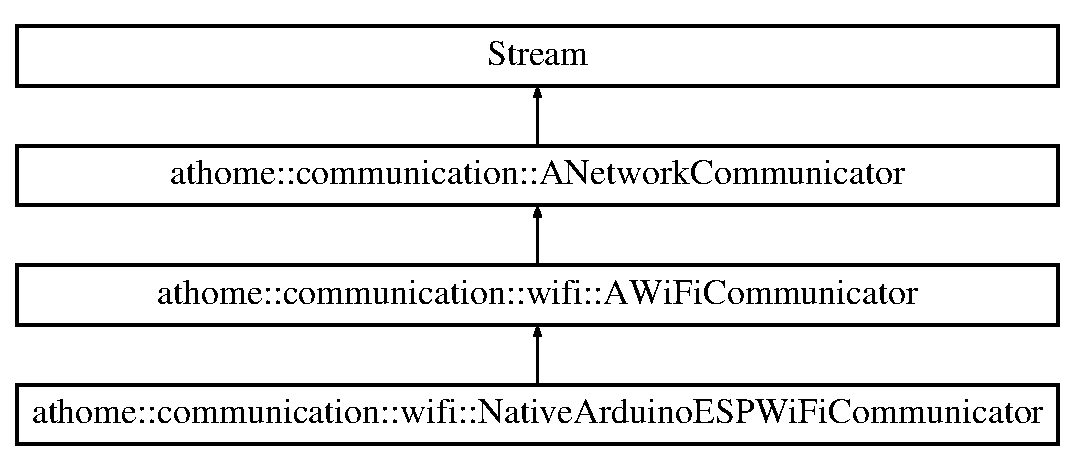
\includegraphics[height=4.000000cm]{classathome_1_1communication_1_1wifi_1_1_native_arduino_e_s_p_wi_fi_communicator}
\end{center}
\end{figure}
\subsection*{Public Member Functions}
\begin{DoxyCompactItemize}
\item 
\mbox{\Hypertarget{classathome_1_1communication_1_1wifi_1_1_native_arduino_e_s_p_wi_fi_communicator_a96875f73157ad5b6f6b903a97638fe05}\label{classathome_1_1communication_1_1wifi_1_1_native_arduino_e_s_p_wi_fi_communicator_a96875f73157ad5b6f6b903a97638fe05}} 
{\bfseries Native\+Arduino\+E\+S\+P\+Wi\+Fi\+Communicator} (const \mbox{\hyperlink{classathome_1_1communication_1_1wifi_1_1_native_arduino_e_s_p_wi_fi_communicator}{Native\+Arduino\+E\+S\+P\+Wi\+Fi\+Communicator}} \&)=delete
\item 
\mbox{\Hypertarget{classathome_1_1communication_1_1wifi_1_1_native_arduino_e_s_p_wi_fi_communicator_a66d9b6a546ec4c054d71a6635a99d2e2}\label{classathome_1_1communication_1_1wifi_1_1_native_arduino_e_s_p_wi_fi_communicator_a66d9b6a546ec4c054d71a6635a99d2e2}} 
\mbox{\hyperlink{classathome_1_1communication_1_1wifi_1_1_native_arduino_e_s_p_wi_fi_communicator}{Native\+Arduino\+E\+S\+P\+Wi\+Fi\+Communicator}} \& {\bfseries operator=} (const \mbox{\hyperlink{classathome_1_1communication_1_1wifi_1_1_native_arduino_e_s_p_wi_fi_communicator}{Native\+Arduino\+E\+S\+P\+Wi\+Fi\+Communicator}} \&)=delete
\item 
virtual int \mbox{\hyperlink{classathome_1_1communication_1_1wifi_1_1_native_arduino_e_s_p_wi_fi_communicator_a6cd3fe64efeb1085c7e6dc71a740a24b}{available}} ()
\item 
virtual int \mbox{\hyperlink{classathome_1_1communication_1_1wifi_1_1_native_arduino_e_s_p_wi_fi_communicator_a07da3b2bf99edad18fb95b6879dbf0f7}{read}} ()
\item 
virtual int \mbox{\hyperlink{classathome_1_1communication_1_1wifi_1_1_native_arduino_e_s_p_wi_fi_communicator_adaa14eb4aa1b147531742c9377aa8db0}{peek}} ()
\item 
virtual size\+\_\+t \mbox{\hyperlink{classathome_1_1communication_1_1wifi_1_1_native_arduino_e_s_p_wi_fi_communicator_a99fab41ad5275649efafa0a776a0348f}{write}} (uint8\+\_\+t)
\item 
virtual void \mbox{\hyperlink{classathome_1_1communication_1_1wifi_1_1_native_arduino_e_s_p_wi_fi_communicator_a5b02865d3bf418d1b4dff8a1198c8dac}{flush}} ()
\item 
virtual int \mbox{\hyperlink{classathome_1_1communication_1_1wifi_1_1_native_arduino_e_s_p_wi_fi_communicator_ab3f6a0e1b9d3be98a876f95dde97976b}{connect\+To\+Host}} ()
\item 
virtual int \mbox{\hyperlink{classathome_1_1communication_1_1wifi_1_1_native_arduino_e_s_p_wi_fi_communicator_a8fa44a5078cb7d61f01b306e1d0d1bfe}{disconnect\+From\+Host}} ()
\item 
virtual int \mbox{\hyperlink{classathome_1_1communication_1_1wifi_1_1_native_arduino_e_s_p_wi_fi_communicator_abc07f2d953fa91f86b8919858e10bbd7}{connect}} ()
\item 
virtual int \mbox{\hyperlink{classathome_1_1communication_1_1wifi_1_1_native_arduino_e_s_p_wi_fi_communicator_a3787e850d48d149ee1392ebfb2920bb3}{disconnect}} ()
\item 
virtual bool \mbox{\hyperlink{classathome_1_1communication_1_1wifi_1_1_native_arduino_e_s_p_wi_fi_communicator_a1ad428f03137d93a142ec5ae72f19e14}{is\+Connected}} () const
\item 
\mbox{\Hypertarget{classathome_1_1communication_1_1wifi_1_1_native_arduino_e_s_p_wi_fi_communicator_a2fbcf882d14174fdcd81aba6a2e7ad54}\label{classathome_1_1communication_1_1wifi_1_1_native_arduino_e_s_p_wi_fi_communicator_a2fbcf882d14174fdcd81aba6a2e7ad54}} 
void {\bfseries set\+Stream\+To\+Chipset} (Stream $\ast$)=delete
\end{DoxyCompactItemize}
\subsection*{Additional Inherited Members}


\subsection{Member Function Documentation}
\mbox{\Hypertarget{classathome_1_1communication_1_1wifi_1_1_native_arduino_e_s_p_wi_fi_communicator_a6cd3fe64efeb1085c7e6dc71a740a24b}\label{classathome_1_1communication_1_1wifi_1_1_native_arduino_e_s_p_wi_fi_communicator_a6cd3fe64efeb1085c7e6dc71a740a24b}} 
\index{athome\+::communication\+::wifi\+::\+Native\+Arduino\+E\+S\+P\+Wi\+Fi\+Communicator@{athome\+::communication\+::wifi\+::\+Native\+Arduino\+E\+S\+P\+Wi\+Fi\+Communicator}!available@{available}}
\index{available@{available}!athome\+::communication\+::wifi\+::\+Native\+Arduino\+E\+S\+P\+Wi\+Fi\+Communicator@{athome\+::communication\+::wifi\+::\+Native\+Arduino\+E\+S\+P\+Wi\+Fi\+Communicator}}
\subsubsection{\texorpdfstring{available()}{available()}}
{\footnotesize\ttfamily int athome\+::communication\+::wifi\+::\+Native\+Arduino\+E\+S\+P\+Wi\+Fi\+Communicator\+::available (\begin{DoxyParamCaption}{ }\end{DoxyParamCaption})\hspace{0.3cm}{\ttfamily [virtual]}}

Virtual method inherited from Stream interface. \href{https://www.arduino.cc/reference/en/language/functions/communication/stream/streamavailable/}{\tt See documentation on Arduino reference.} 

Implements \mbox{\hyperlink{classathome_1_1communication_1_1_a_network_communicator_a2bf367d03c98e8523fda71dd43ffa2fb}{athome\+::communication\+::\+A\+Network\+Communicator}}.

\mbox{\Hypertarget{classathome_1_1communication_1_1wifi_1_1_native_arduino_e_s_p_wi_fi_communicator_abc07f2d953fa91f86b8919858e10bbd7}\label{classathome_1_1communication_1_1wifi_1_1_native_arduino_e_s_p_wi_fi_communicator_abc07f2d953fa91f86b8919858e10bbd7}} 
\index{athome\+::communication\+::wifi\+::\+Native\+Arduino\+E\+S\+P\+Wi\+Fi\+Communicator@{athome\+::communication\+::wifi\+::\+Native\+Arduino\+E\+S\+P\+Wi\+Fi\+Communicator}!connect@{connect}}
\index{connect@{connect}!athome\+::communication\+::wifi\+::\+Native\+Arduino\+E\+S\+P\+Wi\+Fi\+Communicator@{athome\+::communication\+::wifi\+::\+Native\+Arduino\+E\+S\+P\+Wi\+Fi\+Communicator}}
\subsubsection{\texorpdfstring{connect()}{connect()}}
{\footnotesize\ttfamily int athome\+::communication\+::wifi\+::\+Native\+Arduino\+E\+S\+P\+Wi\+Fi\+Communicator\+::connect (\begin{DoxyParamCaption}{ }\end{DoxyParamCaption})\hspace{0.3cm}{\ttfamily [virtual]}}

Virtual method used to implement connection to Wi\+Fi network through the adapter.

A return value of 0 is expected to indicate the connection was successful, otherwise all other values are available for error codes.

Example\+:


\begin{DoxyCode}
\textcolor{preprocessor}{#include <string.h>}
\textcolor{preprocessor}{#include <AtHome.h>}

\textcolor{keyword}{using} \mbox{\hyperlink{structathome_1_1communication_1_1wifi_1_1s__wifi__access__point}{athome::communication::wifi::WiFi\_ap}}; \textcolor{comment}{// Use this to not have to
       write the full namespace names further}
\textcolor{keyword}{using} \mbox{\hyperlink{classathome_1_1communication_1_1wifi_1_1_a_wi_fi_communicator}{athome::communication::wifi::AWiFiCommunicator}};

\textcolor{keywordtype}{void} my\_function\_connecting\_wifi\_to\_network\_called\_foobar(\mbox{\hyperlink{classathome_1_1communication_1_1wifi_1_1_a_wi_fi_communicator_a0098148fe8d0eeee99b7f8f72a72a900}{AWiFiCommunicator}} &wifi) \{
  WiFi\_ap network; \textcolor{comment}{// Declare a WiFi\_ap structure}
  strncpy(network.ssid, \textcolor{stringliteral}{"foobar"}, \textcolor{keyword}{sizeof}(network.ssid)); \textcolor{comment}{// Copy "foobar" in the ssid field of the
       structure, as the SSID of a WiFi network is the name shown to humans}
  strncpy(network.password, \textcolor{stringliteral}{"12345678"}, \textcolor{keyword}{sizeof}(network.password)); \textcolor{comment}{// Copy "12345678" in the password
       field, to set the password used by the WiFi network}
  wifi.setAccessPoint(network); \textcolor{comment}{// Set the WiFi network parameters we created}
  \textcolor{keywordflow}{if} (!wifi.connect()) \{ \textcolor{comment}{// Connect to this network}
    Serial.println(\textcolor{stringliteral}{"Successfully connected to WiFi network"});
  \} \textcolor{keywordflow}{else} \{
    Serial.println(\textcolor{stringliteral}{"Connection to WiFi network failed"});
  \}
\}
\end{DoxyCode}
 

Implements \mbox{\hyperlink{classathome_1_1communication_1_1wifi_1_1_a_wi_fi_communicator_a309927109fbc19aa0fb2afb71d50bbf9}{athome\+::communication\+::wifi\+::\+A\+Wi\+Fi\+Communicator}}.

\mbox{\Hypertarget{classathome_1_1communication_1_1wifi_1_1_native_arduino_e_s_p_wi_fi_communicator_ab3f6a0e1b9d3be98a876f95dde97976b}\label{classathome_1_1communication_1_1wifi_1_1_native_arduino_e_s_p_wi_fi_communicator_ab3f6a0e1b9d3be98a876f95dde97976b}} 
\index{athome\+::communication\+::wifi\+::\+Native\+Arduino\+E\+S\+P\+Wi\+Fi\+Communicator@{athome\+::communication\+::wifi\+::\+Native\+Arduino\+E\+S\+P\+Wi\+Fi\+Communicator}!connect\+To\+Host@{connect\+To\+Host}}
\index{connect\+To\+Host@{connect\+To\+Host}!athome\+::communication\+::wifi\+::\+Native\+Arduino\+E\+S\+P\+Wi\+Fi\+Communicator@{athome\+::communication\+::wifi\+::\+Native\+Arduino\+E\+S\+P\+Wi\+Fi\+Communicator}}
\subsubsection{\texorpdfstring{connect\+To\+Host()}{connectToHost()}}
{\footnotesize\ttfamily int athome\+::communication\+::wifi\+::\+Native\+Arduino\+E\+S\+P\+Wi\+Fi\+Communicator\+::connect\+To\+Host (\begin{DoxyParamCaption}{ }\end{DoxyParamCaption})\hspace{0.3cm}{\ttfamily [virtual]}}

Virtual method used to connect adapter to a socket on a host.

A return value of 0 is expected to indicate success, otherwise all other values are available for error codes.

Example\+:


\begin{DoxyCode}
\textcolor{preprocessor}{#include <AtHome.h>}

\textcolor{keyword}{using} \mbox{\hyperlink{structathome_1_1communication_1_1ip_1_1s__host}{athome::communication::ip::tcp\_host}}; \textcolor{comment}{// Use this to not have to
       write the full namespace names further}
\textcolor{keyword}{using} \mbox{\hyperlink{structathome_1_1communication_1_1wifi_1_1s__wifi__client}{athome::communication::wifi::WiFi\_client}};
\textcolor{keyword}{using} \mbox{\hyperlink{classathome_1_1communication_1_1wifi_1_1_a_wi_fi_communicator}{athome::communication::wifi::AWiFiCommunicator}};

\textcolor{keywordtype}{void} my\_function\_connecting\_to\_http\_port\_on\_router(\mbox{\hyperlink{classathome_1_1communication_1_1wifi_1_1_a_wi_fi_communicator_a0098148fe8d0eeee99b7f8f72a72a900}{AWiFiCommunicator}} &wifi) \{
  \textcolor{keyword}{const} WiFi\_client &my\_ip = wifi.getConnectionAddresses(); \textcolor{comment}{// Get our actual MAC and IP (IPv4 or IPv6)
       addresses}
  tcp\_host router = \{\{my\_ip.ipv4[0], my\_ip.ipv4[1], my\_ip.ipv4[2], 1\}, 80\}; \textcolor{comment}{// Use our current IPv4 address
       to deduce the one of the router, which often is the same as ours but ending with the value 1}
  wifi.setHost(router); \textcolor{comment}{// Set the new host to connect on, our structure tcp\_host is a couple IP + port}
  \textcolor{keywordflow}{if} (!wifi.connectToHost()) \{ \textcolor{comment}{// Connect to the socket on the host}
    Serial.println(\textcolor{stringliteral}{"Successfully connected to host"});
  \} \textcolor{keywordflow}{else} \{
    Serial.println(\textcolor{stringliteral}{"Failed to connect to host"});
  \}
\}
\end{DoxyCode}
 

Implements \mbox{\hyperlink{classathome_1_1communication_1_1_a_network_communicator_a370176dae8f38225446e83a132dbcff7}{athome\+::communication\+::\+A\+Network\+Communicator}}.

\mbox{\Hypertarget{classathome_1_1communication_1_1wifi_1_1_native_arduino_e_s_p_wi_fi_communicator_a3787e850d48d149ee1392ebfb2920bb3}\label{classathome_1_1communication_1_1wifi_1_1_native_arduino_e_s_p_wi_fi_communicator_a3787e850d48d149ee1392ebfb2920bb3}} 
\index{athome\+::communication\+::wifi\+::\+Native\+Arduino\+E\+S\+P\+Wi\+Fi\+Communicator@{athome\+::communication\+::wifi\+::\+Native\+Arduino\+E\+S\+P\+Wi\+Fi\+Communicator}!disconnect@{disconnect}}
\index{disconnect@{disconnect}!athome\+::communication\+::wifi\+::\+Native\+Arduino\+E\+S\+P\+Wi\+Fi\+Communicator@{athome\+::communication\+::wifi\+::\+Native\+Arduino\+E\+S\+P\+Wi\+Fi\+Communicator}}
\subsubsection{\texorpdfstring{disconnect()}{disconnect()}}
{\footnotesize\ttfamily int athome\+::communication\+::wifi\+::\+Native\+Arduino\+E\+S\+P\+Wi\+Fi\+Communicator\+::disconnect (\begin{DoxyParamCaption}{ }\end{DoxyParamCaption})\hspace{0.3cm}{\ttfamily [virtual]}}

Virtual method used to implement disconnection of the current Wi\+Fi network through the adapter.

A return value of 0 is expected to indicate success, otherwise all other values are available for error codes.

Usage is as simple as this\+:


\begin{DoxyCode}
\textcolor{preprocessor}{#include <AWiFiCommunicator.hpp>}

\textcolor{keyword}{using} \mbox{\hyperlink{classathome_1_1communication_1_1wifi_1_1_a_wi_fi_communicator}{athome::communication::wifi::AWiFiCommunicator}};

\textcolor{keywordtype}{void} my\_function\_disconnecting\_wifi\_adapters(AWiFiCommuncator &wifi) \{
  \textcolor{keywordflow}{if} (!wifi.disconnect()) \{
    Serial.println(\textcolor{stringliteral}{"Successfully disconnected from WiFi network"});
  \} \textcolor{keywordflow}{else} \{
    Serial.println(\textcolor{stringliteral}{"Failed to disconnect from WiFi network"}); \textcolor{comment}{// Is that really possible? In case we're
       stuck, it's a problem where the "have you tried turning it off and on again?" rocks ;)}
\}
\end{DoxyCode}
 

Implements \mbox{\hyperlink{classathome_1_1communication_1_1wifi_1_1_a_wi_fi_communicator_a6131240ac0daa0f9fb4d46871feea4c2}{athome\+::communication\+::wifi\+::\+A\+Wi\+Fi\+Communicator}}.

\mbox{\Hypertarget{classathome_1_1communication_1_1wifi_1_1_native_arduino_e_s_p_wi_fi_communicator_a8fa44a5078cb7d61f01b306e1d0d1bfe}\label{classathome_1_1communication_1_1wifi_1_1_native_arduino_e_s_p_wi_fi_communicator_a8fa44a5078cb7d61f01b306e1d0d1bfe}} 
\index{athome\+::communication\+::wifi\+::\+Native\+Arduino\+E\+S\+P\+Wi\+Fi\+Communicator@{athome\+::communication\+::wifi\+::\+Native\+Arduino\+E\+S\+P\+Wi\+Fi\+Communicator}!disconnect\+From\+Host@{disconnect\+From\+Host}}
\index{disconnect\+From\+Host@{disconnect\+From\+Host}!athome\+::communication\+::wifi\+::\+Native\+Arduino\+E\+S\+P\+Wi\+Fi\+Communicator@{athome\+::communication\+::wifi\+::\+Native\+Arduino\+E\+S\+P\+Wi\+Fi\+Communicator}}
\subsubsection{\texorpdfstring{disconnect\+From\+Host()}{disconnectFromHost()}}
{\footnotesize\ttfamily int athome\+::communication\+::wifi\+::\+Native\+Arduino\+E\+S\+P\+Wi\+Fi\+Communicator\+::disconnect\+From\+Host (\begin{DoxyParamCaption}{ }\end{DoxyParamCaption})\hspace{0.3cm}{\ttfamily [virtual]}}

Virtual method to disconnect from the current host, closing the socket.

A return value of 0 is expected to indicate success, otherwise all other values are available for error codes.

Example\+:


\begin{DoxyCode}
\textcolor{preprocessor}{#include <AWiFiCommunicator.hpp>}

\textcolor{keyword}{using} \mbox{\hyperlink{classathome_1_1communication_1_1wifi_1_1_a_wi_fi_communicator}{athome::communication::wifi::AWiFiCommunicator}};

\textcolor{keywordtype}{void} my\_function\_disconnecting\_an\_adapter\_from\_host(\mbox{\hyperlink{classathome_1_1communication_1_1wifi_1_1_a_wi_fi_communicator_a0098148fe8d0eeee99b7f8f72a72a900}{AWiFiCommunicator}} &wifi) \{
  \textcolor{keywordflow}{if} (!wifi.disconnectFromHost()) \{
    Serial.println(\textcolor{stringliteral}{"Successfully disconnected from host"});
  \} \textcolor{keywordflow}{else} \{
    Serial.println(\textcolor{stringliteral}{"Failed to disconnect from host"}); \textcolor{comment}{// If that happens, see the same scenario on
       disconnect method to have the solution ;)}
  \}
\}
\end{DoxyCode}
 

Implements \mbox{\hyperlink{classathome_1_1communication_1_1_a_network_communicator_a025b7fbe9b3c4452fcf1925d766324eb}{athome\+::communication\+::\+A\+Network\+Communicator}}.

\mbox{\Hypertarget{classathome_1_1communication_1_1wifi_1_1_native_arduino_e_s_p_wi_fi_communicator_a5b02865d3bf418d1b4dff8a1198c8dac}\label{classathome_1_1communication_1_1wifi_1_1_native_arduino_e_s_p_wi_fi_communicator_a5b02865d3bf418d1b4dff8a1198c8dac}} 
\index{athome\+::communication\+::wifi\+::\+Native\+Arduino\+E\+S\+P\+Wi\+Fi\+Communicator@{athome\+::communication\+::wifi\+::\+Native\+Arduino\+E\+S\+P\+Wi\+Fi\+Communicator}!flush@{flush}}
\index{flush@{flush}!athome\+::communication\+::wifi\+::\+Native\+Arduino\+E\+S\+P\+Wi\+Fi\+Communicator@{athome\+::communication\+::wifi\+::\+Native\+Arduino\+E\+S\+P\+Wi\+Fi\+Communicator}}
\subsubsection{\texorpdfstring{flush()}{flush()}}
{\footnotesize\ttfamily void athome\+::communication\+::wifi\+::\+Native\+Arduino\+E\+S\+P\+Wi\+Fi\+Communicator\+::flush (\begin{DoxyParamCaption}{ }\end{DoxyParamCaption})\hspace{0.3cm}{\ttfamily [virtual]}}

Virtual method inherited from Stream interface. \href{https://www.arduino.cc/reference/en/language/functions/communication/stream/streamflush/}{\tt See documentation on Arduino reference.} 

Implements \mbox{\hyperlink{classathome_1_1communication_1_1_a_network_communicator_a5e3b278ad11e6c00ac7d3e2fee3f01b1}{athome\+::communication\+::\+A\+Network\+Communicator}}.

\mbox{\Hypertarget{classathome_1_1communication_1_1wifi_1_1_native_arduino_e_s_p_wi_fi_communicator_a1ad428f03137d93a142ec5ae72f19e14}\label{classathome_1_1communication_1_1wifi_1_1_native_arduino_e_s_p_wi_fi_communicator_a1ad428f03137d93a142ec5ae72f19e14}} 
\index{athome\+::communication\+::wifi\+::\+Native\+Arduino\+E\+S\+P\+Wi\+Fi\+Communicator@{athome\+::communication\+::wifi\+::\+Native\+Arduino\+E\+S\+P\+Wi\+Fi\+Communicator}!is\+Connected@{is\+Connected}}
\index{is\+Connected@{is\+Connected}!athome\+::communication\+::wifi\+::\+Native\+Arduino\+E\+S\+P\+Wi\+Fi\+Communicator@{athome\+::communication\+::wifi\+::\+Native\+Arduino\+E\+S\+P\+Wi\+Fi\+Communicator}}
\subsubsection{\texorpdfstring{is\+Connected()}{isConnected()}}
{\footnotesize\ttfamily bool athome\+::communication\+::wifi\+::\+Native\+Arduino\+E\+S\+P\+Wi\+Fi\+Communicator\+::is\+Connected (\begin{DoxyParamCaption}{ }\end{DoxyParamCaption}) const\hspace{0.3cm}{\ttfamily [virtual]}}

Virtual method to know if the adapter is connected to a Wi\+Fi network.

Return true if the adapter is connected, otherwise return false;

Example\+:


\begin{DoxyCode}
\textcolor{preprocessor}{#include <AWiFiCommunicator.hpp>}

\textcolor{keyword}{using} \mbox{\hyperlink{classathome_1_1communication_1_1wifi_1_1_a_wi_fi_communicator}{athome::communication::wifi::AWiFiCommunicator}};

\textcolor{keywordtype}{void} my\_function\_printing\_if\_adapter\_is\_connected\_to\_network\_or\_not(\textcolor{keyword}{const} 
      \mbox{\hyperlink{classathome_1_1communication_1_1wifi_1_1_a_wi_fi_communicator_a0098148fe8d0eeee99b7f8f72a72a900}{AWiFiCommunicator}} &wifi) \{
  Serial.println((wifi.isConnected) ? \textcolor{stringliteral}{"Adapter is connected to WiFi network"} : \textcolor{stringliteral}{"Adapter isn't connected to
       WiFi network"});
\}
\end{DoxyCode}
 

Implements \mbox{\hyperlink{classathome_1_1communication_1_1wifi_1_1_a_wi_fi_communicator_a578087d01c814481d89ea702a6d7ed01}{athome\+::communication\+::wifi\+::\+A\+Wi\+Fi\+Communicator}}.

\mbox{\Hypertarget{classathome_1_1communication_1_1wifi_1_1_native_arduino_e_s_p_wi_fi_communicator_adaa14eb4aa1b147531742c9377aa8db0}\label{classathome_1_1communication_1_1wifi_1_1_native_arduino_e_s_p_wi_fi_communicator_adaa14eb4aa1b147531742c9377aa8db0}} 
\index{athome\+::communication\+::wifi\+::\+Native\+Arduino\+E\+S\+P\+Wi\+Fi\+Communicator@{athome\+::communication\+::wifi\+::\+Native\+Arduino\+E\+S\+P\+Wi\+Fi\+Communicator}!peek@{peek}}
\index{peek@{peek}!athome\+::communication\+::wifi\+::\+Native\+Arduino\+E\+S\+P\+Wi\+Fi\+Communicator@{athome\+::communication\+::wifi\+::\+Native\+Arduino\+E\+S\+P\+Wi\+Fi\+Communicator}}
\subsubsection{\texorpdfstring{peek()}{peek()}}
{\footnotesize\ttfamily int athome\+::communication\+::wifi\+::\+Native\+Arduino\+E\+S\+P\+Wi\+Fi\+Communicator\+::peek (\begin{DoxyParamCaption}{ }\end{DoxyParamCaption})\hspace{0.3cm}{\ttfamily [virtual]}}

Virtual method inherited from Stream interface. \href{https://www.arduino.cc/reference/en/language/functions/communication/stream/streampeek/}{\tt See documentation on Arduino reference.} 

Implements \mbox{\hyperlink{classathome_1_1communication_1_1_a_network_communicator_ad06ecdc94aa77b1bab934b85bed2ac7d}{athome\+::communication\+::\+A\+Network\+Communicator}}.

\mbox{\Hypertarget{classathome_1_1communication_1_1wifi_1_1_native_arduino_e_s_p_wi_fi_communicator_a07da3b2bf99edad18fb95b6879dbf0f7}\label{classathome_1_1communication_1_1wifi_1_1_native_arduino_e_s_p_wi_fi_communicator_a07da3b2bf99edad18fb95b6879dbf0f7}} 
\index{athome\+::communication\+::wifi\+::\+Native\+Arduino\+E\+S\+P\+Wi\+Fi\+Communicator@{athome\+::communication\+::wifi\+::\+Native\+Arduino\+E\+S\+P\+Wi\+Fi\+Communicator}!read@{read}}
\index{read@{read}!athome\+::communication\+::wifi\+::\+Native\+Arduino\+E\+S\+P\+Wi\+Fi\+Communicator@{athome\+::communication\+::wifi\+::\+Native\+Arduino\+E\+S\+P\+Wi\+Fi\+Communicator}}
\subsubsection{\texorpdfstring{read()}{read()}}
{\footnotesize\ttfamily int athome\+::communication\+::wifi\+::\+Native\+Arduino\+E\+S\+P\+Wi\+Fi\+Communicator\+::read (\begin{DoxyParamCaption}{ }\end{DoxyParamCaption})\hspace{0.3cm}{\ttfamily [virtual]}}

Virtual method inherited from Stream interface. \href{https://www.arduino.cc/reference/en/language/functions/communication/stream/streamread/}{\tt See documentation on Arduino reference.} 

Implements \mbox{\hyperlink{classathome_1_1communication_1_1_a_network_communicator_a88d3c4366daf48865ab48b22eb62d610}{athome\+::communication\+::\+A\+Network\+Communicator}}.

\mbox{\Hypertarget{classathome_1_1communication_1_1wifi_1_1_native_arduino_e_s_p_wi_fi_communicator_a99fab41ad5275649efafa0a776a0348f}\label{classathome_1_1communication_1_1wifi_1_1_native_arduino_e_s_p_wi_fi_communicator_a99fab41ad5275649efafa0a776a0348f}} 
\index{athome\+::communication\+::wifi\+::\+Native\+Arduino\+E\+S\+P\+Wi\+Fi\+Communicator@{athome\+::communication\+::wifi\+::\+Native\+Arduino\+E\+S\+P\+Wi\+Fi\+Communicator}!write@{write}}
\index{write@{write}!athome\+::communication\+::wifi\+::\+Native\+Arduino\+E\+S\+P\+Wi\+Fi\+Communicator@{athome\+::communication\+::wifi\+::\+Native\+Arduino\+E\+S\+P\+Wi\+Fi\+Communicator}}
\subsubsection{\texorpdfstring{write()}{write()}}
{\footnotesize\ttfamily size\+\_\+t athome\+::communication\+::wifi\+::\+Native\+Arduino\+E\+S\+P\+Wi\+Fi\+Communicator\+::write (\begin{DoxyParamCaption}\item[{uint8\+\_\+t}]{ }\end{DoxyParamCaption})\hspace{0.3cm}{\ttfamily [virtual]}}

Virtual method inherited from Stream interface. \href{https://www.arduino.cc/en/Serial/Write}{\tt See documentation on Arduino reference.} 

Implements \mbox{\hyperlink{classathome_1_1communication_1_1_a_network_communicator_a87adf68359a4ec5b0a38bea529ebf732}{athome\+::communication\+::\+A\+Network\+Communicator}}.



The documentation for this class was generated from the following files\+:\begin{DoxyCompactItemize}
\item 
src/Native\+Arduino\+E\+S\+P\+Wi\+Fi\+Communicator.\+hpp\item 
src/communication/network/wifi/Native\+Arduino\+E\+S\+P\+Wi\+Fi\+Communicator.\+cpp\end{DoxyCompactItemize}

\hypertarget{structathome_1_1display_1_1_grove_chainable_l_e_d_1_1_pins}{}\section{athome\+:\+:display\+:\+:Grove\+Chainable\+L\+ED\+:\+:Pins Struct Reference}
\label{structathome_1_1display_1_1_grove_chainable_l_e_d_1_1_pins}\index{athome\+::display\+::\+Grove\+Chainable\+L\+E\+D\+::\+Pins@{athome\+::display\+::\+Grove\+Chainable\+L\+E\+D\+::\+Pins}}
\subsection*{Public Attributes}
\begin{DoxyCompactItemize}
\item 
\mbox{\Hypertarget{structathome_1_1display_1_1_grove_chainable_l_e_d_1_1_pins_aeb0cdc4f20d987807ffb35deae4fa322}\label{structathome_1_1display_1_1_grove_chainable_l_e_d_1_1_pins_aeb0cdc4f20d987807ffb35deae4fa322}} 
uint8\+\_\+t {\bfseries clock}
\item 
\mbox{\Hypertarget{structathome_1_1display_1_1_grove_chainable_l_e_d_1_1_pins_ae8603cd9e402170a5f575a1cc16c5d11}\label{structathome_1_1display_1_1_grove_chainable_l_e_d_1_1_pins_ae8603cd9e402170a5f575a1cc16c5d11}} 
uint8\+\_\+t {\bfseries data}
\end{DoxyCompactItemize}


The documentation for this struct was generated from the following file\+:\begin{DoxyCompactItemize}
\item 
src/Grove\+Chainable\+L\+E\+D.\+hpp\end{DoxyCompactItemize}

\hypertarget{structathome_1_1power_1_1_i_power_1_1_power_info}{}\section{athome\+:\+:power\+:\+:I\+Power\+:\+:Power\+Info Struct Reference}
\label{structathome_1_1power_1_1_i_power_1_1_power_info}\index{athome\+::power\+::\+I\+Power\+::\+Power\+Info@{athome\+::power\+::\+I\+Power\+::\+Power\+Info}}
\subsection*{Public Attributes}
\begin{DoxyCompactItemize}
\item 
\mbox{\Hypertarget{structathome_1_1power_1_1_i_power_1_1_power_info_a62f956c304f45bb1b89eb81cc0c13845}\label{structathome_1_1power_1_1_i_power_1_1_power_info_a62f956c304f45bb1b89eb81cc0c13845}} 
uint32\+\_\+t {\bfseries voltage}
\item 
\mbox{\Hypertarget{structathome_1_1power_1_1_i_power_1_1_power_info_a45db3bab2d10641ead505cb2a9177e10}\label{structathome_1_1power_1_1_i_power_1_1_power_info_a45db3bab2d10641ead505cb2a9177e10}} 
uint32\+\_\+t {\bfseries current}
\item 
\mbox{\Hypertarget{structathome_1_1power_1_1_i_power_1_1_power_info_a05e86772e61fa527dff5c2e4673ef9a9}\label{structathome_1_1power_1_1_i_power_1_1_power_info_a05e86772e61fa527dff5c2e4673ef9a9}} 
uint8\+\_\+t {\bfseries remaining\+Capacity}
\end{DoxyCompactItemize}


The documentation for this struct was generated from the following file\+:\begin{DoxyCompactItemize}
\item 
src/I\+Power.\+hpp\end{DoxyCompactItemize}

\hypertarget{classathome_1_1display_1_1_p_w_m_l_e_d}{}\section{athome\+:\+:display\+:\+:P\+W\+M\+L\+ED Class Reference}
\label{classathome_1_1display_1_1_p_w_m_l_e_d}\index{athome\+::display\+::\+P\+W\+M\+L\+ED@{athome\+::display\+::\+P\+W\+M\+L\+ED}}
Inheritance diagram for athome\+:\+:display\+:\+:P\+W\+M\+L\+ED\+:\begin{figure}[H]
\begin{center}
\leavevmode
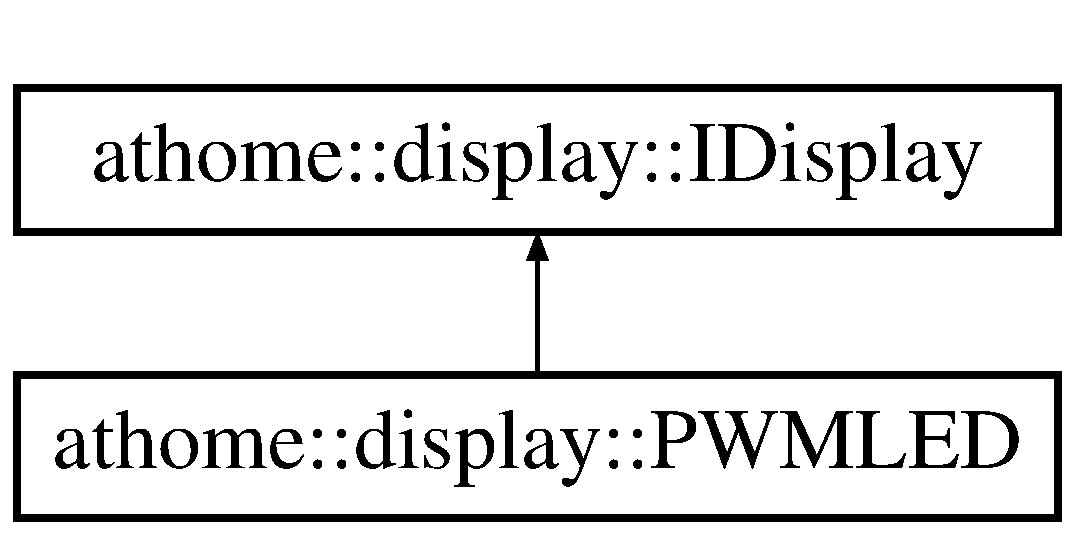
\includegraphics[height=2.000000cm]{classathome_1_1display_1_1_p_w_m_l_e_d}
\end{center}
\end{figure}
\subsection*{Public Member Functions}
\begin{DoxyCompactItemize}
\item 
\mbox{\Hypertarget{classathome_1_1display_1_1_p_w_m_l_e_d_a5c38a60e95d6c6b6c29bc6ba8d138690}\label{classathome_1_1display_1_1_p_w_m_l_e_d_a5c38a60e95d6c6b6c29bc6ba8d138690}} 
{\bfseries P\+W\+M\+L\+ED} (int, bool=false)
\item 
\mbox{\Hypertarget{classathome_1_1display_1_1_p_w_m_l_e_d_a581dc9e092c193ef2fa19eb889a62c32}\label{classathome_1_1display_1_1_p_w_m_l_e_d_a581dc9e092c193ef2fa19eb889a62c32}} 
{\bfseries P\+W\+M\+L\+ED} (const \mbox{\hyperlink{classathome_1_1display_1_1_p_w_m_l_e_d}{P\+W\+M\+L\+ED}} \&)=delete
\item 
\mbox{\Hypertarget{classathome_1_1display_1_1_p_w_m_l_e_d_a66e47914fd9e6e836de8cc18732deadf}\label{classathome_1_1display_1_1_p_w_m_l_e_d_a66e47914fd9e6e836de8cc18732deadf}} 
\mbox{\hyperlink{classathome_1_1display_1_1_p_w_m_l_e_d}{P\+W\+M\+L\+ED}} \& {\bfseries operator=} (const \mbox{\hyperlink{classathome_1_1display_1_1_p_w_m_l_e_d}{P\+W\+M\+L\+ED}} \&)=delete
\item 
virtual void \mbox{\hyperlink{classathome_1_1display_1_1_p_w_m_l_e_d_ad13265bec1900a48d3d89aac9a532783}{clear}} ()
\item 
virtual void \mbox{\hyperlink{classathome_1_1display_1_1_p_w_m_l_e_d_a49a059d9bbd5bf08c0e057f0c957e736}{update}} ()
\item 
virtual void \mbox{\hyperlink{classathome_1_1display_1_1_p_w_m_l_e_d_a8cde32d9aa5b28dfbc79e2677bfce921}{set\+Displayed\+Estimate}} (\mbox{\hyperlink{classathome_1_1sensor_1_1_i_sensor_aa70bc27a4c17c86caf96cca776541ddf}{sensor\+::\+I\+Sensor\+::\+I\+Sensor\+Scale}})
\end{DoxyCompactItemize}


\subsection{Member Function Documentation}
\mbox{\Hypertarget{classathome_1_1display_1_1_p_w_m_l_e_d_ad13265bec1900a48d3d89aac9a532783}\label{classathome_1_1display_1_1_p_w_m_l_e_d_ad13265bec1900a48d3d89aac9a532783}} 
\index{athome\+::display\+::\+P\+W\+M\+L\+ED@{athome\+::display\+::\+P\+W\+M\+L\+ED}!clear@{clear}}
\index{clear@{clear}!athome\+::display\+::\+P\+W\+M\+L\+ED@{athome\+::display\+::\+P\+W\+M\+L\+ED}}
\subsubsection{\texorpdfstring{clear()}{clear()}}
{\footnotesize\ttfamily void athome\+::display\+::\+P\+W\+M\+L\+E\+D\+::clear (\begin{DoxyParamCaption}{ }\end{DoxyParamCaption})\hspace{0.3cm}{\ttfamily [virtual]}}

Remove display content 

Implements \mbox{\hyperlink{classathome_1_1display_1_1_i_display_a0d3add1ce61c96657827fb56d250d9c6}{athome\+::display\+::\+I\+Display}}.

\mbox{\Hypertarget{classathome_1_1display_1_1_p_w_m_l_e_d_a8cde32d9aa5b28dfbc79e2677bfce921}\label{classathome_1_1display_1_1_p_w_m_l_e_d_a8cde32d9aa5b28dfbc79e2677bfce921}} 
\index{athome\+::display\+::\+P\+W\+M\+L\+ED@{athome\+::display\+::\+P\+W\+M\+L\+ED}!set\+Displayed\+Estimate@{set\+Displayed\+Estimate}}
\index{set\+Displayed\+Estimate@{set\+Displayed\+Estimate}!athome\+::display\+::\+P\+W\+M\+L\+ED@{athome\+::display\+::\+P\+W\+M\+L\+ED}}
\subsubsection{\texorpdfstring{set\+Displayed\+Estimate()}{setDisplayedEstimate()}}
{\footnotesize\ttfamily void athome\+::display\+::\+P\+W\+M\+L\+E\+D\+::set\+Displayed\+Estimate (\begin{DoxyParamCaption}\item[{\mbox{\hyperlink{classathome_1_1sensor_1_1_i_sensor_aa70bc27a4c17c86caf96cca776541ddf}{sensor\+::\+I\+Sensor\+::\+I\+Sensor\+Scale}}}]{ }\end{DoxyParamCaption})\hspace{0.3cm}{\ttfamily [virtual]}}

Set the value displayed on the screen, whatever the type of display is.

I\+Sensor\+Scale is an enumeration representing the correctness on a scale from 1 to 10 (1 is worst, 10 is best).

This scale can be represented by various ways for many different displays. For example\+:


\begin{DoxyItemize}
\item An L\+ED could stay off from 6 and on below 6
\item A dimmable L\+ED could set it\textquotesingle{}s percentage of brightness corresponding to the value (for example 1 = 100\%, 5 = 50\%, 10 = 0\%)
\item A 7 segments display could display the digit itself and stay off at 10
\item An L\+CD screen could write a sentence, the digit, draw a gauge, ...etc
\item A speaker or buzzer could do noise of different intensities below 6
\item ...etc 
\end{DoxyItemize}

Implements \mbox{\hyperlink{classathome_1_1display_1_1_i_display_a3c9678f929e4bc04742d458b0c2399ef}{athome\+::display\+::\+I\+Display}}.

\mbox{\Hypertarget{classathome_1_1display_1_1_p_w_m_l_e_d_a49a059d9bbd5bf08c0e057f0c957e736}\label{classathome_1_1display_1_1_p_w_m_l_e_d_a49a059d9bbd5bf08c0e057f0c957e736}} 
\index{athome\+::display\+::\+P\+W\+M\+L\+ED@{athome\+::display\+::\+P\+W\+M\+L\+ED}!update@{update}}
\index{update@{update}!athome\+::display\+::\+P\+W\+M\+L\+ED@{athome\+::display\+::\+P\+W\+M\+L\+ED}}
\subsubsection{\texorpdfstring{update()}{update()}}
{\footnotesize\ttfamily void athome\+::display\+::\+P\+W\+M\+L\+E\+D\+::update (\begin{DoxyParamCaption}{ }\end{DoxyParamCaption})\hspace{0.3cm}{\ttfamily [virtual]}}

Update display content 

Implements \mbox{\hyperlink{classathome_1_1display_1_1_i_display_a4ba7bd5d46f88578f1c846f4f5f3c5d1}{athome\+::display\+::\+I\+Display}}.



The documentation for this class was generated from the following files\+:\begin{DoxyCompactItemize}
\item 
src/P\+W\+M\+L\+E\+D.\+hpp\item 
src/display/P\+W\+M\+L\+E\+D.\+cpp\end{DoxyCompactItemize}

\hypertarget{structathome_1_1communication_1_1ip_1_1s__host}{}\section{athome\+:\+:communication\+:\+:ip\+:\+:s\+\_\+host Struct Reference}
\label{structathome_1_1communication_1_1ip_1_1s__host}\index{athome\+::communication\+::ip\+::s\+\_\+host@{athome\+::communication\+::ip\+::s\+\_\+host}}
\subsection*{Public Attributes}
\begin{DoxyCompactItemize}
\item 
\mbox{\Hypertarget{structathome_1_1communication_1_1ip_1_1s__host_a729beda2149b1c34039edbcfc794ab96}\label{structathome_1_1communication_1_1ip_1_1s__host_a729beda2149b1c34039edbcfc794ab96}} 
\begin{tabbing}
xx\=xx\=xx\=xx\=xx\=xx\=xx\=xx\=xx\=\kill
union \{\\
\>ipv6\_address {\bfseries ipv6}\\
\>ipv4\_address {\bfseries ipv4}\\
\}; \\

\end{tabbing}\item 
\mbox{\Hypertarget{structathome_1_1communication_1_1ip_1_1s__host_a676f8f8134a3ef8bb3363c71488d1da2}\label{structathome_1_1communication_1_1ip_1_1s__host_a676f8f8134a3ef8bb3363c71488d1da2}} 
port {\bfseries hport}
\end{DoxyCompactItemize}


The documentation for this struct was generated from the following file\+:\begin{DoxyCompactItemize}
\item 
src/Network\+I\+P\+Types.\+hpp\end{DoxyCompactItemize}

\hypertarget{structathome_1_1communication_1_1wifi_1_1s__wifi__access__point}{}\section{athome\+:\+:communication\+:\+:wifi\+:\+:s\+\_\+wifi\+\_\+access\+\_\+point Struct Reference}
\label{structathome_1_1communication_1_1wifi_1_1s__wifi__access__point}\index{athome\+::communication\+::wifi\+::s\+\_\+wifi\+\_\+access\+\_\+point@{athome\+::communication\+::wifi\+::s\+\_\+wifi\+\_\+access\+\_\+point}}
\subsection*{Public Attributes}
\begin{DoxyCompactItemize}
\item 
\mbox{\Hypertarget{structathome_1_1communication_1_1wifi_1_1s__wifi__access__point_a215e9c0f8f72c926110bc7f46360e1ea}\label{structathome_1_1communication_1_1wifi_1_1s__wifi__access__point_a215e9c0f8f72c926110bc7f46360e1ea}} 
wifi\+\_\+ssid {\bfseries ssid}
\item 
\mbox{\Hypertarget{structathome_1_1communication_1_1wifi_1_1s__wifi__access__point_a13c710aba9ae52ad4360c667c914b988}\label{structathome_1_1communication_1_1wifi_1_1s__wifi__access__point_a13c710aba9ae52ad4360c667c914b988}} 
wifi\+\_\+password {\bfseries password}
\item 
\mbox{\Hypertarget{structathome_1_1communication_1_1wifi_1_1s__wifi__access__point_accf0d6bf42e6d30be881bf9247200c73}\label{structathome_1_1communication_1_1wifi_1_1s__wifi__access__point_accf0d6bf42e6d30be881bf9247200c73}} 
wifi\+\_\+channel {\bfseries channel}
\item 
\mbox{\Hypertarget{structathome_1_1communication_1_1wifi_1_1s__wifi__access__point_acbae620a23b6d1a0dd073597f5e167bf}\label{structathome_1_1communication_1_1wifi_1_1s__wifi__access__point_acbae620a23b6d1a0dd073597f5e167bf}} 
wifi\+\_\+norm {\bfseries norm}
\item 
\mbox{\Hypertarget{structathome_1_1communication_1_1wifi_1_1s__wifi__access__point_af738ada78d21e0c9d70b3d713bfd708c}\label{structathome_1_1communication_1_1wifi_1_1s__wifi__access__point_af738ada78d21e0c9d70b3d713bfd708c}} 
wifi\+\_\+frequency\+\_\+band {\bfseries band}
\end{DoxyCompactItemize}


The documentation for this struct was generated from the following file\+:\begin{DoxyCompactItemize}
\item 
Wi\+Fi\+Types.\+hpp\end{DoxyCompactItemize}

\hypertarget{structathome_1_1communication_1_1wifi_1_1s__wifi__client}{}\section{athome\+:\+:communication\+:\+:wifi\+:\+:s\+\_\+wifi\+\_\+client Struct Reference}
\label{structathome_1_1communication_1_1wifi_1_1s__wifi__client}\index{athome\+::communication\+::wifi\+::s\+\_\+wifi\+\_\+client@{athome\+::communication\+::wifi\+::s\+\_\+wifi\+\_\+client}}
\subsection*{Public Attributes}
\begin{DoxyCompactItemize}
\item 
\mbox{\Hypertarget{structathome_1_1communication_1_1wifi_1_1s__wifi__client_a47f84e7a3151ffbd74d4c92a5aa74f2d}\label{structathome_1_1communication_1_1wifi_1_1s__wifi__client_a47f84e7a3151ffbd74d4c92a5aa74f2d}} 
ip\+::mac\+\_\+address {\bfseries mac}
\item 
\mbox{\Hypertarget{structathome_1_1communication_1_1wifi_1_1s__wifi__client_a0fc3a6574b5350548c665c79adce737f}\label{structathome_1_1communication_1_1wifi_1_1s__wifi__client_a0fc3a6574b5350548c665c79adce737f}} 
\begin{tabbing}
xx\=xx\=xx\=xx\=xx\=xx\=xx\=xx\=xx\=\kill
union \{\\
\>ip::ipv4\_address {\bfseries ipv4}\\
\>ip::ipv6\_address {\bfseries ipv6}\\
\}; \\

\end{tabbing}\end{DoxyCompactItemize}


The documentation for this struct was generated from the following file\+:\begin{DoxyCompactItemize}
\item 
src/Wi\+Fi\+Types.\+hpp\end{DoxyCompactItemize}

\hypertarget{classathome_1_1sensor_1_1_sound_sensor}{}\section{athome\+:\+:sensor\+:\+:Sound\+Sensor Class Reference}
\label{classathome_1_1sensor_1_1_sound_sensor}\index{athome\+::sensor\+::\+Sound\+Sensor@{athome\+::sensor\+::\+Sound\+Sensor}}
Inheritance diagram for athome\+:\+:sensor\+:\+:Sound\+Sensor\+:\begin{figure}[H]
\begin{center}
\leavevmode
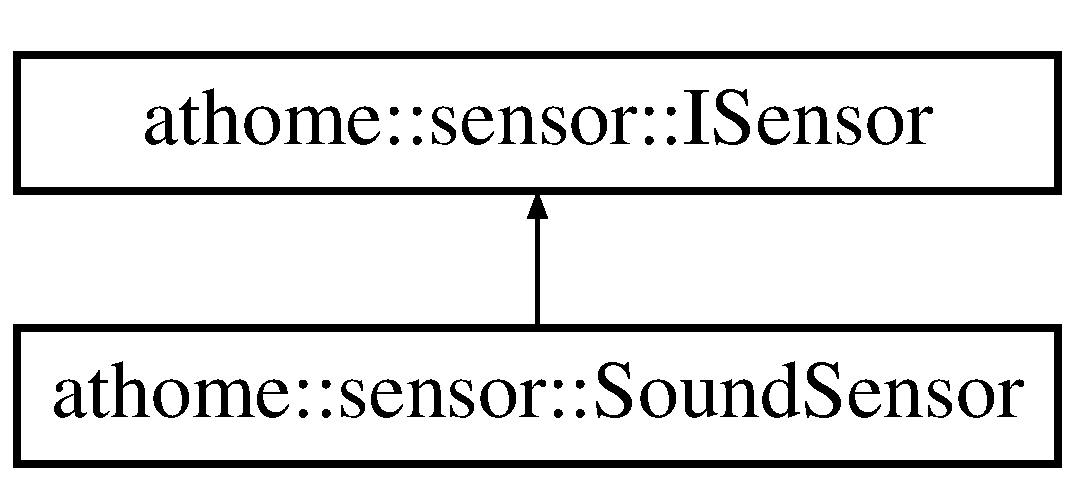
\includegraphics[height=2.000000cm]{classathome_1_1sensor_1_1_sound_sensor}
\end{center}
\end{figure}
\subsection*{Public Member Functions}
\begin{DoxyCompactItemize}
\item 
\mbox{\Hypertarget{classathome_1_1sensor_1_1_sound_sensor_affd617ff59a1354519c01b812b805568}\label{classathome_1_1sensor_1_1_sound_sensor_affd617ff59a1354519c01b812b805568}} 
{\bfseries Sound\+Sensor} (int pin)
\item 
\mbox{\Hypertarget{classathome_1_1sensor_1_1_sound_sensor_a581afa638adb939d606dbfbe1d419628}\label{classathome_1_1sensor_1_1_sound_sensor_a581afa638adb939d606dbfbe1d419628}} 
{\bfseries Sound\+Sensor} (const \mbox{\hyperlink{classathome_1_1sensor_1_1_sound_sensor}{Sound\+Sensor}} \&)=delete
\item 
\mbox{\Hypertarget{classathome_1_1sensor_1_1_sound_sensor_ab974a1520aaf9497611445dfc523ad32}\label{classathome_1_1sensor_1_1_sound_sensor_ab974a1520aaf9497611445dfc523ad32}} 
\mbox{\hyperlink{classathome_1_1sensor_1_1_sound_sensor}{Sound\+Sensor}} \& {\bfseries operator=} (const \mbox{\hyperlink{classathome_1_1sensor_1_1_sound_sensor}{Sound\+Sensor}} \&)=delete
\item 
const I\+Sensor\+Value \& \mbox{\hyperlink{classathome_1_1sensor_1_1_sound_sensor_a8ac5f417eee873247aff8a7e96e12817}{get\+Sample}} ()
\item 
void \mbox{\hyperlink{classathome_1_1sensor_1_1_sound_sensor_adaf42abe0443f486361656efe9587ba7}{set\+Thresholds}} (const \mbox{\hyperlink{structathome_1_1sensor_1_1_i_sensor_1_1_i_sensor_thresholds}{I\+Sensor\+Thresholds}} \&thresholds)
\item 
\mbox{\Hypertarget{classathome_1_1sensor_1_1_sound_sensor_a225996767d89ef25e039ccddfab16bfc}\label{classathome_1_1sensor_1_1_sound_sensor_a225996767d89ef25e039ccddfab16bfc}} 
void {\bfseries set\+Pin} (int pin)
\item 
\mbox{\Hypertarget{classathome_1_1sensor_1_1_sound_sensor_ae4c3496911502614bef9a00195653800}\label{classathome_1_1sensor_1_1_sound_sensor_ae4c3496911502614bef9a00195653800}} 
int {\bfseries get\+Pin} () const
\end{DoxyCompactItemize}
\subsection*{Additional Inherited Members}


\subsection{Member Function Documentation}
\mbox{\Hypertarget{classathome_1_1sensor_1_1_sound_sensor_a8ac5f417eee873247aff8a7e96e12817}\label{classathome_1_1sensor_1_1_sound_sensor_a8ac5f417eee873247aff8a7e96e12817}} 
\index{athome\+::sensor\+::\+Sound\+Sensor@{athome\+::sensor\+::\+Sound\+Sensor}!get\+Sample@{get\+Sample}}
\index{get\+Sample@{get\+Sample}!athome\+::sensor\+::\+Sound\+Sensor@{athome\+::sensor\+::\+Sound\+Sensor}}
\subsubsection{\texorpdfstring{get\+Sample()}{getSample()}}
{\footnotesize\ttfamily const I\+Sensor\+Value\& athome\+::sensor\+::\+Sound\+Sensor\+::get\+Sample (\begin{DoxyParamCaption}{ }\end{DoxyParamCaption})\hspace{0.3cm}{\ttfamily [inline]}, {\ttfamily [virtual]}}

Returns a pointer on sensor sample raw memory, as an array of bytes 

Implements \mbox{\hyperlink{classathome_1_1sensor_1_1_i_sensor_ae109cd3741ea9c88dc7e4f2eaf1485d5}{athome\+::sensor\+::\+I\+Sensor}}.

\mbox{\Hypertarget{classathome_1_1sensor_1_1_sound_sensor_adaf42abe0443f486361656efe9587ba7}\label{classathome_1_1sensor_1_1_sound_sensor_adaf42abe0443f486361656efe9587ba7}} 
\index{athome\+::sensor\+::\+Sound\+Sensor@{athome\+::sensor\+::\+Sound\+Sensor}!set\+Thresholds@{set\+Thresholds}}
\index{set\+Thresholds@{set\+Thresholds}!athome\+::sensor\+::\+Sound\+Sensor@{athome\+::sensor\+::\+Sound\+Sensor}}
\subsubsection{\texorpdfstring{set\+Thresholds()}{setThresholds()}}
{\footnotesize\ttfamily void athome\+::sensor\+::\+Sound\+Sensor\+::set\+Thresholds (\begin{DoxyParamCaption}\item[{const \mbox{\hyperlink{structathome_1_1sensor_1_1_i_sensor_1_1_i_sensor_thresholds}{I\+Sensor\+Thresholds}} \&}]{ }\end{DoxyParamCaption})\hspace{0.3cm}{\ttfamily [inline]}, {\ttfamily [virtual]}}

Returns the estimation of safety from the current sensor value

Example\+:


\begin{DoxyCode}
\textcolor{keywordtype}{void} my\_function\_telling\_if\_a\_sensor\_value\_is\_good\_or\_not(ISensor
&my\_sensor) \{ \mbox{\hyperlink{classathome_1_1sensor_1_1_i_sensor_aa70bc27a4c17c86caf96cca776541ddf}{ISensorScale}} sensor\_estimate = my\_sensor.getEstimate(); \textcolor{keywordflow}{if}
(sensor\_estimate == ISensor::ZERO) \{ Serial.println(\textcolor{stringliteral}{"The sensor returned an}
\textcolor{stringliteral}{invalid value"});
  \}
  \textcolor{keywordflow}{else} \textcolor{keywordflow}{if} (sensor\_estimate > ISensor::ZERO && sensor\_estimate < 6) \{
    Serial.println(\textcolor{stringliteral}{"Boouh, it's not good :("});
  \}
  \textcolor{keywordflow}{else} \{
    Serial.println(\textcolor{stringliteral}{"Yaaaay!"});
  \}
\}
\end{DoxyCode}
 

Implements \mbox{\hyperlink{classathome_1_1sensor_1_1_i_sensor_af86df8538fecfcfc670b4adfbbde6abb}{athome\+::sensor\+::\+I\+Sensor}}.



The documentation for this class was generated from the following file\+:\begin{DoxyCompactItemize}
\item 
src/Sound\+Sensor.\+hpp\end{DoxyCompactItemize}

\hypertarget{classathome_1_1sensor_1_1_thermistor}{}\section{athome\+:\+:sensor\+:\+:Thermistor$<$ R1, R2, R3, P\+R\+EC, V\+R\+EF, R\+R\+EF $>$ Class Template Reference}
\label{classathome_1_1sensor_1_1_thermistor}\index{athome\+::sensor\+::\+Thermistor$<$ R1, R2, R3, P\+R\+E\+C, V\+R\+E\+F, R\+R\+E\+F $>$@{athome\+::sensor\+::\+Thermistor$<$ R1, R2, R3, P\+R\+E\+C, V\+R\+E\+F, R\+R\+E\+F $>$}}


{\ttfamily \#include $<$Thermistor.\+hpp$>$}

Inheritance diagram for athome\+:\+:sensor\+:\+:Thermistor$<$ R1, R2, R3, P\+R\+EC, V\+R\+EF, R\+R\+EF $>$\+:\begin{figure}[H]
\begin{center}
\leavevmode
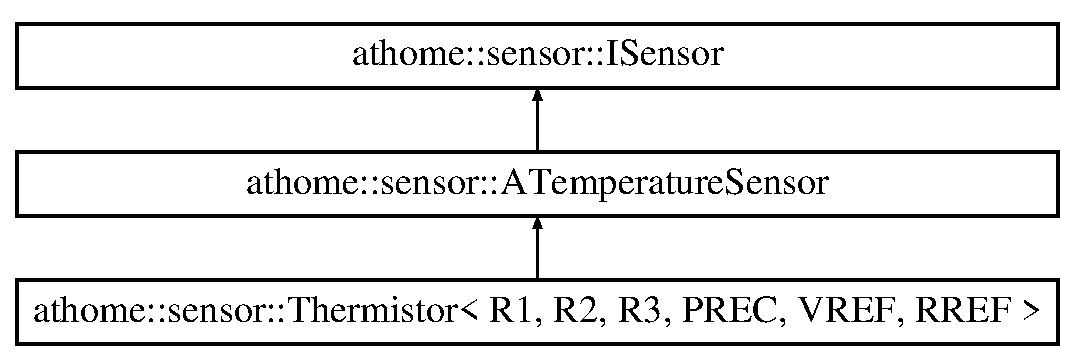
\includegraphics[height=3.000000cm]{classathome_1_1sensor_1_1_thermistor}
\end{center}
\end{figure}
\subsection*{Public Member Functions}
\begin{DoxyCompactItemize}
\item 
\mbox{\Hypertarget{classathome_1_1sensor_1_1_thermistor_a44767c962e57aa33ef6fd10ea3b00cf9}\label{classathome_1_1sensor_1_1_thermistor_a44767c962e57aa33ef6fd10ea3b00cf9}} 
{\bfseries Thermistor} (int pin)
\item 
\mbox{\Hypertarget{classathome_1_1sensor_1_1_thermistor_a3cbfb96cd205f2ddb6fa813b4dedbafe}\label{classathome_1_1sensor_1_1_thermistor_a3cbfb96cd205f2ddb6fa813b4dedbafe}} 
{\bfseries Thermistor} (const \mbox{\hyperlink{classathome_1_1sensor_1_1_thermistor}{Thermistor}} \&)=delete
\item 
\mbox{\Hypertarget{classathome_1_1sensor_1_1_thermistor_a7820ca124e20e1a1665a8b5c2cdce71f}\label{classathome_1_1sensor_1_1_thermistor_a7820ca124e20e1a1665a8b5c2cdce71f}} 
\mbox{\hyperlink{classathome_1_1sensor_1_1_thermistor}{Thermistor}} \& {\bfseries operator=} (const \mbox{\hyperlink{classathome_1_1sensor_1_1_thermistor}{Thermistor}} \&)=delete
\item 
virtual int32\+\_\+t \mbox{\hyperlink{classathome_1_1sensor_1_1_thermistor_abc45d8d277fb186b5d303f9e53bf73d4}{get\+Sensor\+Sample}} ()
\end{DoxyCompactItemize}
\subsection*{Additional Inherited Members}


\subsection{Detailed Description}
\subsubsection*{template$<$uint32\+\_\+t R1, uint32\+\_\+t R2, uint32\+\_\+t R3, size\+\_\+t P\+R\+EC = 1024, uint8\+\_\+t V\+R\+EF = 5, uint32\+\_\+t R\+R\+EF = 10000$>$\newline
class athome\+::sensor\+::\+Thermistor$<$ R1, R2, R3, P\+R\+E\+C, V\+R\+E\+F, R\+R\+E\+F $>$}

Based on Steinhart-\/\+Hart equation\+:


\begin{DoxyItemize}
\item T1 = 5 degree celsius
\item T2 = 25 degree celsius
\item T3 = 50 degree celsius
\end{DoxyItemize}

T\+O\+DO\+: Need to update it to use the static version of log function once implemented 

\subsection{Member Function Documentation}
\mbox{\Hypertarget{classathome_1_1sensor_1_1_thermistor_abc45d8d277fb186b5d303f9e53bf73d4}\label{classathome_1_1sensor_1_1_thermistor_abc45d8d277fb186b5d303f9e53bf73d4}} 
\index{athome\+::sensor\+::\+Thermistor@{athome\+::sensor\+::\+Thermistor}!get\+Sensor\+Sample@{get\+Sensor\+Sample}}
\index{get\+Sensor\+Sample@{get\+Sensor\+Sample}!athome\+::sensor\+::\+Thermistor@{athome\+::sensor\+::\+Thermistor}}
\subsubsection{\texorpdfstring{get\+Sensor\+Sample()}{getSensorSample()}}
{\footnotesize\ttfamily template$<$uint32\+\_\+t R1, uint32\+\_\+t R2, uint32\+\_\+t R3, size\+\_\+t P\+R\+EC = 1024, uint8\+\_\+t V\+R\+EF = 5, uint32\+\_\+t R\+R\+EF = 10000$>$ \\
virtual int32\+\_\+t \mbox{\hyperlink{classathome_1_1sensor_1_1_thermistor}{athome\+::sensor\+::\+Thermistor}}$<$ R1, R2, R3, P\+R\+EC, V\+R\+EF, R\+R\+EF $>$\+::get\+Sensor\+Sample (\begin{DoxyParamCaption}{ }\end{DoxyParamCaption})\hspace{0.3cm}{\ttfamily [inline]}, {\ttfamily [virtual]}}

Returns the last value sampled from the sensor (do not actually resample it). 

Implements \mbox{\hyperlink{classathome_1_1sensor_1_1_a_temperature_sensor_a4e5b2c79ab69f6903f7b322da45b0af4}{athome\+::sensor\+::\+A\+Temperature\+Sensor}}.



The documentation for this class was generated from the following file\+:\begin{DoxyCompactItemize}
\item 
src/Thermistor.\+hpp\end{DoxyCompactItemize}

\hypertarget{classathome_1_1sensor_1_1_t_m_p36_g_z_temperature_sensor}{}\section{athome\+:\+:sensor\+:\+:T\+M\+P36\+G\+Z\+Temperature\+Sensor$<$ R\+EF, R\+ES $>$ Class Template Reference}
\label{classathome_1_1sensor_1_1_t_m_p36_g_z_temperature_sensor}\index{athome\+::sensor\+::\+T\+M\+P36\+G\+Z\+Temperature\+Sensor$<$ R\+E\+F, R\+E\+S $>$@{athome\+::sensor\+::\+T\+M\+P36\+G\+Z\+Temperature\+Sensor$<$ R\+E\+F, R\+E\+S $>$}}
Inheritance diagram for athome\+:\+:sensor\+:\+:T\+M\+P36\+G\+Z\+Temperature\+Sensor$<$ R\+EF, R\+ES $>$\+:\begin{figure}[H]
\begin{center}
\leavevmode
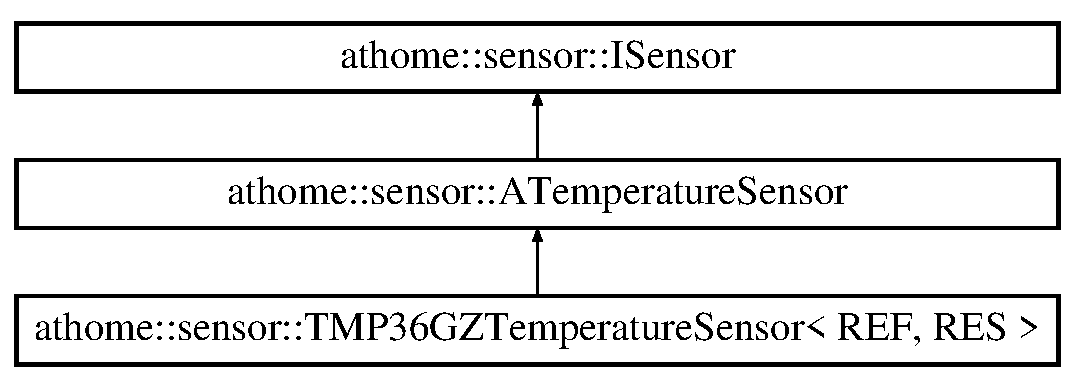
\includegraphics[height=3.000000cm]{classathome_1_1sensor_1_1_t_m_p36_g_z_temperature_sensor}
\end{center}
\end{figure}
\subsection*{Public Member Functions}
\begin{DoxyCompactItemize}
\item 
\mbox{\Hypertarget{classathome_1_1sensor_1_1_t_m_p36_g_z_temperature_sensor_a8da15abb0144a1074956dc39a10b0d8c}\label{classathome_1_1sensor_1_1_t_m_p36_g_z_temperature_sensor_a8da15abb0144a1074956dc39a10b0d8c}} 
{\bfseries T\+M\+P36\+G\+Z\+Temperature\+Sensor} (uint8\+\_\+t pin)
\item 
\mbox{\Hypertarget{classathome_1_1sensor_1_1_t_m_p36_g_z_temperature_sensor_ac5a99d97f0a19f10bb5cba8dc22d620b}\label{classathome_1_1sensor_1_1_t_m_p36_g_z_temperature_sensor_ac5a99d97f0a19f10bb5cba8dc22d620b}} 
{\bfseries T\+M\+P36\+G\+Z\+Temperature\+Sensor} (const \mbox{\hyperlink{classathome_1_1sensor_1_1_t_m_p36_g_z_temperature_sensor}{T\+M\+P36\+G\+Z\+Temperature\+Sensor}} \&)=delete
\item 
\mbox{\Hypertarget{classathome_1_1sensor_1_1_t_m_p36_g_z_temperature_sensor_a56a451e62807f163dba052f35adc6bc7}\label{classathome_1_1sensor_1_1_t_m_p36_g_z_temperature_sensor_a56a451e62807f163dba052f35adc6bc7}} 
\mbox{\hyperlink{classathome_1_1sensor_1_1_t_m_p36_g_z_temperature_sensor}{T\+M\+P36\+G\+Z\+Temperature\+Sensor}} \& {\bfseries operator=} (const \mbox{\hyperlink{classathome_1_1sensor_1_1_t_m_p36_g_z_temperature_sensor}{T\+M\+P36\+G\+Z\+Temperature\+Sensor}} \&)=delete
\item 
int32\+\_\+t \mbox{\hyperlink{classathome_1_1sensor_1_1_t_m_p36_g_z_temperature_sensor_ae0e101ee54c5c64842d2cab9fb9292f4}{get\+Sensor\+Sample}} ()
\end{DoxyCompactItemize}
\subsection*{Additional Inherited Members}


\subsection{Member Function Documentation}
\mbox{\Hypertarget{classathome_1_1sensor_1_1_t_m_p36_g_z_temperature_sensor_ae0e101ee54c5c64842d2cab9fb9292f4}\label{classathome_1_1sensor_1_1_t_m_p36_g_z_temperature_sensor_ae0e101ee54c5c64842d2cab9fb9292f4}} 
\index{athome\+::sensor\+::\+T\+M\+P36\+G\+Z\+Temperature\+Sensor@{athome\+::sensor\+::\+T\+M\+P36\+G\+Z\+Temperature\+Sensor}!get\+Sensor\+Sample@{get\+Sensor\+Sample}}
\index{get\+Sensor\+Sample@{get\+Sensor\+Sample}!athome\+::sensor\+::\+T\+M\+P36\+G\+Z\+Temperature\+Sensor@{athome\+::sensor\+::\+T\+M\+P36\+G\+Z\+Temperature\+Sensor}}
\subsubsection{\texorpdfstring{get\+Sensor\+Sample()}{getSensorSample()}}
{\footnotesize\ttfamily template$<$uint32\+\_\+t R\+EF, uint8\+\_\+t R\+ES$>$ \\
int32\+\_\+t \mbox{\hyperlink{classathome_1_1sensor_1_1_t_m_p36_g_z_temperature_sensor}{athome\+::sensor\+::\+T\+M\+P36\+G\+Z\+Temperature\+Sensor}}$<$ R\+EF, R\+ES $>$\+::get\+Sensor\+Sample (\begin{DoxyParamCaption}{ }\end{DoxyParamCaption})\hspace{0.3cm}{\ttfamily [inline]}, {\ttfamily [virtual]}}

Returns the last value sampled from the sensor (do not actually resample it). 

Implements \mbox{\hyperlink{classathome_1_1sensor_1_1_a_temperature_sensor_a4e5b2c79ab69f6903f7b322da45b0af4}{athome\+::sensor\+::\+A\+Temperature\+Sensor}}.



The documentation for this class was generated from the following file\+:\begin{DoxyCompactItemize}
\item 
src/T\+M\+P36\+G\+Z\+Temperature\+Sensor.\+hpp\end{DoxyCompactItemize}

\hypertarget{structathome_1_1utility_1_1units_1_1_unit}{}\section{athome\+:\+:utility\+:\+:units\+:\+:Unit Struct Reference}
\label{structathome_1_1utility_1_1units_1_1_unit}\index{athome\+::utility\+::units\+::\+Unit@{athome\+::utility\+::units\+::\+Unit}}
\subsection*{Public Attributes}
\begin{DoxyCompactItemize}
\item 
\mbox{\Hypertarget{structathome_1_1utility_1_1units_1_1_unit_ad627fbae275f81a1632daf0d80769b1c}\label{structathome_1_1utility_1_1units_1_1_unit_ad627fbae275f81a1632daf0d80769b1c}} 
uint8\+\_\+t {\bfseries unit}
\item 
\mbox{\Hypertarget{structathome_1_1utility_1_1units_1_1_unit_a8c99ee8bca4e320323ccbb358eddb284}\label{structathome_1_1utility_1_1units_1_1_unit_a8c99ee8bca4e320323ccbb358eddb284}} 
uint8\+\_\+t {\bfseries prefix}
\end{DoxyCompactItemize}


The documentation for this struct was generated from the following file\+:\begin{DoxyCompactItemize}
\item 
src/At\+Home\+Units.\+hpp\end{DoxyCompactItemize}

\hypertarget{structathome_1_1sensor_1_1_m_q2_gas_sensor_1_1_values}{}\section{athome\+:\+:sensor\+:\+:M\+Q2\+Gas\+Sensor\+:\+:Values Struct Reference}
\label{structathome_1_1sensor_1_1_m_q2_gas_sensor_1_1_values}\index{athome\+::sensor\+::\+M\+Q2\+Gas\+Sensor\+::\+Values@{athome\+::sensor\+::\+M\+Q2\+Gas\+Sensor\+::\+Values}}
\subsection*{Public Attributes}
\begin{DoxyCompactItemize}
\item 
\mbox{\Hypertarget{structathome_1_1sensor_1_1_m_q2_gas_sensor_1_1_values_ab4c361d142adf2606b02abe045c9e879}\label{structathome_1_1sensor_1_1_m_q2_gas_sensor_1_1_values_ab4c361d142adf2606b02abe045c9e879}} 
int {\bfseries lpg}
\item 
\mbox{\Hypertarget{structathome_1_1sensor_1_1_m_q2_gas_sensor_1_1_values_afb7043620ff1fb73d8529005b84cc979}\label{structathome_1_1sensor_1_1_m_q2_gas_sensor_1_1_values_afb7043620ff1fb73d8529005b84cc979}} 
int {\bfseries co}
\item 
\mbox{\Hypertarget{structathome_1_1sensor_1_1_m_q2_gas_sensor_1_1_values_a2a653baf83c9be7b6e417da6ae54e769}\label{structathome_1_1sensor_1_1_m_q2_gas_sensor_1_1_values_a2a653baf83c9be7b6e417da6ae54e769}} 
int {\bfseries smoke}
\end{DoxyCompactItemize}


The documentation for this struct was generated from the following file\+:\begin{DoxyCompactItemize}
\item 
src/M\+Q2\+Gas\+Sensor.\+hpp\end{DoxyCompactItemize}

%--- End generated contents ---

% Index
\backmatter
\newpage
\phantomsection
\clearemptydoublepage
\addcontentsline{toc}{chapter}{Index}
\printindex

\end{document}
